%!TEX spellcheck = en_US
\documentclass[]{tommaso-thesis}

\usepackage{graphicx}\graphicspath{{Images/}}
\usepackage{tabularx, paralist}
\usepackage[table]{xcolor}
\usepackage[draft]{fixme}
%\usepackage{tikz}
%\usetikzlibrary{automata}
%\usepackage{setspace}
%\setstretch{1.05}

%\usepackage{amssymb}
\usepackage{listings, xspace, url, colortbl, wrapfig,  ifthen, multirow, rotating}
%float,
\usepackage{cancel}

%change 'sl' to 'bf' for bold, or 'normalfont' for no special
%formatting
\captionsetup{labelfont={sl,sf}}

\lstdefinelanguage{algebra}
{morekeywords={import,sort,constructors,observers,transformers,axioms,if,
else,end},
sensitive=false,
morecomment=[l]{//s},
}


%\title{A Bug With A Suit---\\Deep Models For Tracking Issue}
\title{Augmenting Software Development \\with Reified Execution Data}
%\subtitle{Subtitle: Reinventing the World} %optional
\author{Tommaso Dal Sasso}
\advisor{Prof. Dr. Michele Lanza}

\Day{Yesterday} %compulsory
\Month{September} %compulsory
\Year{2017} %compulsory, put only the year
\place{Lugano} %compulsory

\programDirector{The PhD program Director \emph{pro tempore}} %compulsory
%\programDirectorA{Prof. Walter Binder} %compulsory
%\programDirectorB{Prof. Michael Bronstein} %compulsory


\committee{%
  \committeeMember{Mehdi Jazayeri}{Universit\`a della Svizzera Italiana, Switzerland}
  \committeeMember{Cesare Pautasso}{Universit\`a della Svizzera Italiana, Switzerland}

  \committeeMember{Martin Pinzger}{Alpen-Adria-Universit\"at, Austria}
  \committeeMember{Rocco Oliveto}{University of Molise, Italy}
  \committeeMember{Andy Zaidman}{Delft University of Technology, The Netherlands}
}

\dedication{To my beloved} %optional
\openepigraph{%Someone said \dots}{Someone} %optional
Alice: But I don't want to go among mad people!

Cheshire Cat: Oh, you can't help that. Most everyone's mad here.
You may have noticed that I'm not all there myself.}
{Alice in Wonderland}


\makeindex %optional, also comment out \theindex at the end

%!TEX root = tommaso-thesis.tex
%!TEX spellcheck = en_US
\usepackage{xspace}

\newcommand{\bzilla}{\textsc{Bugzilla}\xspace}
\newcommand{\jira}{\textsc{JIRA}\xspace}
\newcommand{\gth}{\textsc{GitHub}\xspace}
\newcommand{\fbz}{\textsc{FogBugz}\xspace}
\newcommand{\ib}{\textsc{In*Bug}\xspace}
\newcommand{\sln}{\textsc{ShoreLine}\xspace}
\newcommand{\slr}{\textsc{ShoreLine Reporter}\xspace}
\newcommand{\bea}{\textsc{Beacon}\xspace}
\newcommand{\dfl}{\textsc{DFlow}\xspace}
\newcommand{\pha}{\textsc{Pharo}\xspace}
\newcommand{\sea}{\textsc{Seaside}\xspace}

\newcommand{\mypar}[1]{\paragraph{\textbf{#1.}}}
\newcommand{\structure}{\subsubsection*{Structure of the Chapter}}

\newcommand{\entity}[1]{\textsc{#1}\xspace}
\newcommand{\method}[1]{\textit{#1}\xspace}

% \renewcommand{\cite}[1]{[#1]}
%\newboolean{showcomments}
%\setboolean{showcomments}{true}
%\ifthenelse{\boolean{showcomments}}
%  {\newcommand{\nb}[2]{\fbox{\bfseries\sffamily\scriptsize#1}{\sf\small$\blacktriangleright$\textit{#2}$\blacktriangleleft$}}}
%  {\newcommand{\nb}[2]{}}
%\newcommand\TLN[1]{\nb{Michele}{#1}}
%\newcommand\AM[1]{\nb{Andrea}{#1}}
%\newcommand\TDS[1]{\nb{Tommaso}{#1}}


%%% Colors %%%
% model
\definecolor{gray50}{gray}{.5}
\definecolor{gray40}{gray}{.6}
\definecolor{gray30}{gray}{.7}
\definecolor{gray20}{gray}{.8}
\definecolor{gray10}{gray}{.9}
\definecolor{gray05}{gray}{.95}

%%% Gamification %%%
\definecolor{oceanboatblue}{rgb}{0.0, 0.47, 0.75}
\definecolor{red-brown}{rgb}{0.65, 0.16, 0.16}
\definecolor{citrine}{RGB}{249, 214, 157}
\definecolor{tanzanite}{RGB}{203, 205, 222}
\definecolor{quartz}{RGB}{231, 206, 218}
\definecolor{jade}{RGB}{178, 223, 178}
\definecolor{topaz}{RGB}{173, 214, 244}
\definecolor{amethyst}{RGB}{230, 169, 252}
\definecolor{ruby}{RGB}{250, 142, 169}
\definecolor{emerald}{RGB}{157, 216, 191}
\definecolor{aquamarine}{RGB}{176, 215, 228}
\definecolor{sapphire}{RGB}{35, 23, 197}
\definecolor{gold}{rgb}{1.0, 0.84, 0.0}


\newcommand{\buildingblock}[2]{
    \begin{wrapfigure}{l}{0.10\linewidth}
    	\vspace{-15pt}
    	\begin{center}
    	\includegraphics[width=\linewidth]{gamification/#2}
    	\end{center}
    	\vspace{-15pt}
    \end{wrapfigure}

    \noindent\textbf{#1:}
}

\newcommand{\badge}[1]{
\noindent
\begin{wrapfigure}{l}{0.07\textwidth}
  \vspace{-18pt}
  \begin{center}
    \includegraphics[width=0.06\textwidth]{gamification/#1.pdf}
  \end{center}
  \vspace{-20pt}
\end{wrapfigure}
}


\begin{document}

\maketitle %generates the titlepage, this is FIXED

\frontmatter %generates the frontmatter, this is FIXED


%!TEX root = ../tommaso-thesis.tex
%!TEX spellcheck = en_US

\begin{abstract}
%Software development has become a prominent activity, with influence in almost every human activity.
Software development has become more and more pervasive, with influence in almost every human activity.
To be able to fit in so many different scenarios and constantly implement new features, software developers adopted methodologies with tight development cycles, sometimes with more than one release per day.
%Software development is an activity centered around the continuous modification of source code to implement new features, improve the current behavior, and correct defects.
With the constant growth of modern software projects and the consequent expansion of development teams, understanding all the components of a system becomes a task too big to handle.

In this context understanding the cause of an error or identifying its source is not an easy task, and correcting the erroneous behavior can lead to unexpected downtime of vital services.
Being able to keep track of software defects, usually referred to as \emph{bugs}, is crucial in the development of a project and in containing maintenance costs.
For this purpose, the correctness and completeness of the information available has a great impact on the time required to understand and solve a problem.

In this thesis we present an overview of the current techniques commonly used to report software defects.
We show why we believe that the state of the art needs to be improved, and
% what approach we suggest in dealing with this kind of data.
% We
present a set of approaches and tools to collect data from software failures, model it, and turn it into actionable knowledge.
Our goal is to show that data generated from errors can have a great impact on daily software development, and how it can be employed to augment the development environment to assist software engineers to build and maintain software systems.

\end{abstract}


%!TEX root = tommaso-thesis.tex
%!TEX spellcheck = en_US

\begin{acknowledgements}

It should not come as a surprise that the years during a PhD are the most intense during one's life.
Many crossed my path during these years and contributed in shaping this experience.
I thank you all for what you gave me: I hope I was able to gift you at least a spark of inspiration.

Thanks to Michele...

A big thank to the REVEALers, in particular its \emph{hard core} members: Andrea, Luca, and Roberto, who shared with me the journey from the beginning.
I loved you. And I hated you. Often both at the same time.


Thanks to the Pharo community

Thanks to the people in charge of making badges at the conferences I attended.
I have rarely seen matched the creativity that you constantly put in finding new ways of writing my name.
I have to admit it: ``Sasso, Tommaso Dal'' is a masterpiece.


\end{acknowledgements}




\tableofcontents
\listoffigures %optional
\listoftables %optional

\mainmatter

\part{Introduction}
  %!TEX root = ../tommaso-thesis.tex
%!TEX spellcheck = en_US

\chapter{Introduction}\label{ch:introduction}

Everybody uses software.
Maybe it is a control system for the production environment of a large factory.
Maybe it is the interface to access a professional knowledge base, or a social network.
Maybe it is an application on a smartphone, or a website to book a flight.

Regardless of its use, software plays a central role in modern society: It is used in almost any human activity, allowing users to automate the most trivial tasks.
Its usage became massively pervasive, to the point where virtually any structured activity and process relies on software to regulate its workflow, minimize errors, and reduce costs.
Moreover, the surge of popularity of mobile computing pushed even further the momentum of this flourishing scenario, and pushed the influence of software deeper into every aspect of our lives.

To keep pace with such a vibrant landscape, development teams have to write code fast and push new features in a short period of time.
All these changes in the codebase cause systems to constantly change and evolve their behavior, sometimes more than once a day.
Often changes are performed by different developers, or even by different teams working on different parts of the system: Therefore, it quickly becomes impossible for a single person to grasp comprehension of the whole system.
It is easy to understand how a software system can gradually start to resemble an unknown black box, rather than a deterministic process.

To complicate things even further, a deep knowledge of the whole set of components that form a system is often not sufficient to predict its final behavior.
Given the large number of requirements that modern software systems have to satisfy, it is usually necessary to rely on external libraries to provide the desired features.
Using external code is a good practice, as it allows for reuse and reduces the probability of a bug being present in a library used by more people.
However, these benefits come at the cost of yielding control of the system to external code, leading the consequence that, if an error arises from a library, it becomes virtually impossible to track down its origin unless by debugging the library itself.

The main focus during a development cycle is writing new code to develop new features: However, in such a complex and ever-changing scenario, a huge part of the resources put in a project are spent in maintenance and debugging~\cite{Corb1989,Fjel1983,Zelk1979,Mine2015b}.
We can break down the constituent components of maintenance in: finding and collecting problems, understanding them, locating the source of the infection, and fixing the issue.
Each one of these phases comes with its own set of problems and complexities.

In such a scenario, one would imagine that the effort for providing means to aid developers would focus on refined tools to navigate, understand, and inspect the code.
While this is partly true, many of the modern editors and IDEs put the biggest accent on how developers write code, leaving program comprehension as a secondary task, despite it being intrinsically more complicated.


\section{The Problem of Dealing With Code}

%%%%%%%%%%%%%%%%%%%%%%%%%%%%%%%%%
%\mypar{The Curse of Text}
It is easy to see why understanding software is hard: Reading code requires reading text that contains structured information in a language that does not follow the same logic of natural language. To understand a fragment of code, a developer has to mentally parse a source file, identify and extract the necessary information, and build a \emph{mental model} of the (intended) behavior of the software. The same process happens when printing log messages to expose the state of the system: Log messages embody fragments of information that the developer has to fit into her mental model, and use it to reverse engineer the source of an error by trial and error.

To ease this process, both researchers and industry built a plethora of tools like debuggers and code inspectors, that allow developers to run a program in a controlled environment, and to check the internal status of its variables.
Other tools, like code browsers, support fast linking between the entities in the code, while loggers allow to print and store useful runtime information.
Finally, test suites allow to define a set of expected behaviors, and to constantly check if any of these rules is satisfied.

All these tools however do not change the fundamental way we interact with the code: Eventually, the developer needs to read the code, and therefore undergo the process of building its mental model.
This is because all these tools rely on the same, strong, underlying assumption: Source code is text, therefore the tools we are using to interact with it are shaped around text editing tools.
This assumption reflects the way we use to store our programs, \ie plain-text files containing the declaration of our models.

%We propose a novel approach for runtime data collection: We advocate the use of objects to store information about an exception, in order to preserve the multidimensional nature of the information, and leverage the implicit properties that can be obtained by the data structure. By describing errors as first-class citizens of a system, and using a storage format that does not flatten the information, we can reify logs and leverage their expressive power to support a number of development activities. A structured data source allows to build a set of specialized tools to browse the data in an incremental fashion, to discover its implicit structure, or to enable the use of automated analysis, mitigating the need of a data cleaning phase. It can also be stored and sent for debugging purposes, thus creating bug reports with a much higher level of detail and reliability than simple plain text.

%%%%%%%%%%%%%%%%%%%%%%%%%%%%%%%%%


\section{Thesis Statement}\label{sec:thesis}

-Our thesis is...

\begin{framed}
The information produced during the failure of a program contains valuable insights about the whole system, that is conveyed both by its contents and by its structure.
This information cannot be effectively expressed using plain text.
%The format we use to store this information must express both.
\end{framed}


\section{Contributions}

What we did.


\section{Outline}

In \chpref{chp:stacktraces}

  %!TEX root = ../tommaso-thesis.tex
%!TEX spellcheck = en_US

\chapter{State of the Art}\label{ch:related}

% \section{History of the Issue Tracking Systems}

% In the beginning it was text.
% Then became the bug.

The correctness of a computer program is obviously an essential requisite for it to work.
However, it is nearly impossible to determine that a non-trivial program is really correct: the huge amount of different variables and environments to which a program gets usually exposed makes predicting all the potentially harmful situations a hard task.
Moreover, the fact that a program appears as correct at a given time does not guarantee that it will continue behaving correctly also in the future: several factors such as a change in the underlying technology, like the operating system, or different usage conditions like a change in the input format, can cause the arise of problems that were not predicted nor observed before.
For this reason, since we cannot get rid of bugs, dealing efficiently with defects is a crucial component in the success of a software system.

Since the beginning of the history of computer programming, developers needed a procedure to track and describe the appearance, impact, and resolution of the errors encountered during the evolution of a system.
\figref{fig:first-bug-report} shows what the folklore considers to be the first bug report, written by Grace Hopper.
Since that handwritten sheet of paper, issue trackers evolved and adapted to reflect the different development practices introduced during the years.
This led to a well established de facto model of a bug report.
In this chapter we illustrate the state of the art in issue tracking, providing an overview on the current tools and practices and the approaches they propose, to identify the useful elements in issue tracking.

\begin{figure}[t]
\centering
  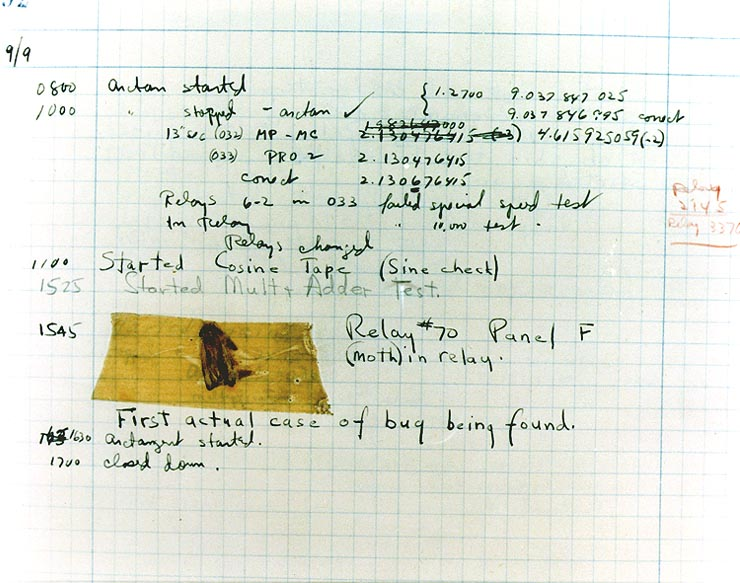
\includegraphics[width=.7\linewidth]{related/bug}
  \caption[The first "bug" report.]{This piece of paper is considered to be the first "bug" report. It was written by Grace Hopper when she was working on the Mark II computer, to document the find of a moth that caused a malfunction in the system.\footnote{\url{http://ei.cs.vt.edu/~history/Hopper.Danis.html}}}
  \label{fig:first-bug-report}
\end{figure}




\section{Issue Tracking Systems}\label{sec:related-bugtrackers}

\begin{figure}[t]
%\begin{wrapfigure}[14]{r}{0.45\textwidth}
\centering
  \vspace{-12pt}
  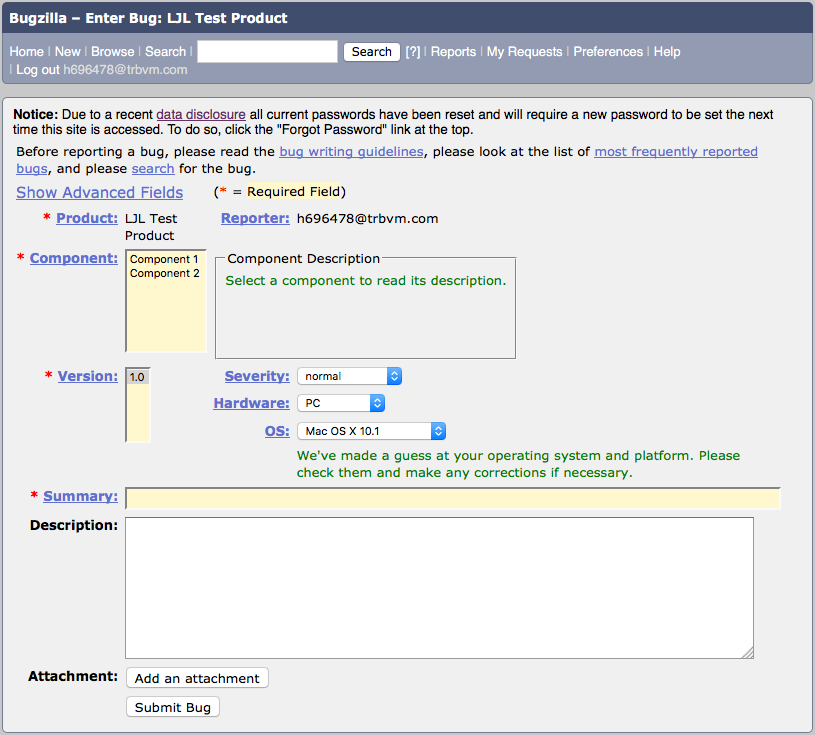
\includegraphics[width=.7\linewidth]{related/bugzilla}
  \caption{An old Bugzilla submission form}
  \label{fig:bugzilla-interface}
%\end{wrapfigure}
\end{figure}

In 1998, the Mozilla Foundation released the first version of Bugzilla, which would soon become the reference issue tracking system.
During the years different alternative tools emerged, providing their own set of customizations and personalizations.
In this section we present four platforms, selected by importance and overall adoption, showing their salient features: Bugzilla, Jira, the GitHub issue tracker and FogBugz.


\subsection{Bugzilla}

Bugzilla \seeurl{https://www.bugzilla.org} is one of the oldest and most popular issue tracking systems, that inspired many existing issue trackers. Developed by the Mozilla Foundation, it is used by several open source projects, as well as industrial customers. Bugzilla allows its users to obtain a great level of detail in specifying an issue, thus producing, however, a complex interface, as shown in \figref{fig:bugzilla-interface}.


\subsection{JIRA}

Jira by Atlassian\seeurl{https://www.atlassian.com/software/jira} is one of the most famous commercial issue trackers, used by Twitter, Linkedin, and Ebay. It provides a polished interface and strong integration with the tools developed by the company. It uses a model similar to Bugzilla.

% \begin{wrapfigure}[9]{r}{0.45\textwidth}
\begin{figure}[t]
\centering
 \includegraphics[width=.95\linewidth]{related/github}
 \caption{GitHub bug report submission form}
 \label{fig:github-interface}
% \end{wrapfigure}
\end{figure}

\subsection{GitHub} GitHub is a popular \texttt{Git} repository hosting service, used to develop several popular open source projects, that offers a simple issue tracker. GitHub adopts a simplified model of a bug report, but offers a strong integration with the versioned source code, by linking issues with specific commits.

%\paragraph{\bf FogBugz.} \fbz\seeurl{https://www.fogcreek.com/fogbugz} is an issue tracker developed by FogCreek. I uses a bug model similar to Bugzilla, slightly polished and user-friendly, due to its clean user interface and advanced filtering capabilities. It poses a strong accent on customization, by letting users define custom filters and views.

\paragraph{}
%\bf Other platforms}
Together with these platform, the open source and commercial scenes provide other popular solutions, like FogBugz, Redmine or Trac\footnote{\url{https://www.fogcreek.com/fogbugz}, \url{https://redmine.org/}, \url{http://trac.edgewall.org/}}. It is however interesting to observe that, while these systems propose different degrees of integration with the tools in their ecosystem (\eg the versioning system), the fundamental approach they adopt follows the same paradigm made popular by Bugzilla: a textual description with additional customizable metadata. Further improvements to issue trackers, and the research around them, are built on top of this paradigm. In the following section, we present the efforts to improve issue trackers and their use in support the bug fixing activity.


\section{Bug Reports}

Dealing with bug reports is a non-trivial task, that poses a number of communication problems among users and developers. Such a large, noisy, and sometimes redundant corpus of information, impacts the debugging time and the maintenance costs. To minimize this impact, researchers focused on improving several aspects of this process. In the following, we present the results of research in selected areas, that represent the core aspects to compose a smart issue tracking system.


\subsection{Quality of a Bug Report}

The reliability and completeness of bug reports is crucial to quickly solve a defect. Bissyande \etal showed that most reporters that contribute to a project are not developers~\cite{Biss2013}, posing a problem on the quality of the data. To understand how developers perceive the quality of a bug report, researchers conducted a survey, asking which elements help understanding a problem. They found that stack traces are the most useful item and often contribute to a faster resolution of a defect, suggesting that they should be collected and included in issue trackers~\cite{Zimm2010a,Bett2007,Schr2010a}. Even when reliable, though, the amount of information in an issue tracker can hide the relevant information: To alleviate the information overload, Sun devised a technique to detect bug reports without useful information~\cite{Sun2011}. Besides incorrect information, bug repositories often contain duplicate entries for the same defect. However, developers do not consider this harmful, but instead find the additional information useful to better understand the problem~\cite{Bett2008a}.
%\paragraph{\bf Automating the Information Management.}

Managing a large bug repository is often a burden that adds a new layer of complexity on top of the bug fixing problem. To alleviate this burden, researchers proposed to use automated approaches~\cite{Weim2006}. For example, Anvik \etal observed that large open source projects are often overwhelmed by the rate of new bug reports and proposed a machine learning based approach to to aid bug \emph{triaging} decisions~\cite{Anvi2006a}, the process of selecting the a the right person to take care of an issue.

%Guo \etal conducted a study to predict what impacts the resolution time of \textit{MS Windows} bug reports~\cite{Guo2010}, finding that a high number of reassignment of a report usually increases the issue lifetime, and that the reputation of the submitter also impacts the fixing time. Given the expensive nature of the bug fixing activity, a number of approaches exist to estimate the cost of a bug fix in person-hours~\cite{Weis2007}, predict bug fixing time~\cite{Gige2010}, locate features from bug reports \cite{Dit2013a}, and perform traceability linking \cite{Biss2013a}.


\subsection{Relevance of Bug Reports}

An important element to reduce the time needed to close a defect comes not only from filtering the relevant reports inside issue trackers, but also from the collection of valuable information.
To support the reliability of the collected information, both researchers and developers implemented tools to collect runtime exceptions to analyze runtime errors. For example, Glerum \etal used an automated approach to leverage the errors collected through WER, the \emph{Windows Error Reporting} tool~\cite{Glerum2009}. In their approach they grouped these reports into buckets, that they used to prioritize debugging and build a knowledge base where system administrators could check common problems of the system. Han Shi~\etal applied the same principle to performance debugging~\cite{Han2012}: They proposed an approach called \textsc{StackMine}, designed to detect and report performance bugs and address defects that cause delays in the user experience. Mozilla adopts a similar approach to collect stack traces and for debugging purposes~\cite{McLa2004}.

The information of stack traces contained in bug reports represents a valuable support in debugging: as such, many researchers devised different methods to aid bug fixing and management of reports using stack traces. These studies provided evidence that stack traces are useful tools and a precious source of information~\cite{Davie2013,Wang2013,Brod2005,Weis2007a}, as they provide precise information, usually more reliable and useful than the descriptions produced by the submitter of a bug report~\cite{Ko2006}. Moreno \etal applied Text Retrieval techniques to compute similarity between bug reports using the stack traces in the report description, focusing on reducing the overhead to analyze large amounts of data~\cite{Moreno2014}.

%We believe that collecting stack traces and leveraging runtime data is a valuable support for developers in a programming environment, and should be part of the standard set of features of an issue tracking system.



\subsection{Understanding Bug Reports}

Having obtained meaningful and reliable data, it is important to build tools to make use of this information. Accessing the information in a bug report is a difficult step in the debugging process: The large amount of information and the reliability of the data reported by the users, consume a significative amount of developers' time. To alleviate this burden, researchers devised a number of approaches based on the visualization of the data inside issue trackers. D'Ambros \etal analyzed the Bugzilla bug repository and synthesized a state transitions diagram of a report~\cite{DAmb2007b}. They built visualizations to support the analysis of a bug database at different levels of granularity, that depicts bug reports as independent entities. Their approach allows users to browse the history of an issue tracker and inspect parts of the system with custom filters. Knab \etal proposed visualizations to ease the understanding of the data in an issue tracker and find hidden patterns~\cite{Knab2009a,Knab2010a}. Hora \etal proposed a visual exploration of the bug repository, considering bugs as first class entities, and linking them to other software artifacts~\cite{Hora2012a}. All these approaches focus on retrospective analyses. We believe that while conceptually interesting, there is little practical utility in daily development, since after all the goal of an issue tracking system is not to look at defects, but to actually fix them. This implies that even the most elaborated techniques are of limited actionability, since the bug fixing process takes place in a different space, namely the integrated development environment (IDE). We believe that the use for a visualization is not to simply display the data, but to establish a first-class link to the development environment.


\subsection{Bug Prediction}

Solving defects does not represent the end of life of the information inside issue trackers: Yin \etal show the danger of hidden complexity behind a bug report, finding that 4.8\% to 24.4\% of sampled fixes for post-release bugs introduced new defects~\cite{Yin2011a}. They also noted that ``Developers and reviewers for incorrect fixes usually do not have enough knowledge about the involved code'', and that ``27\% of the incorrect fixes are made by developers who have never touched the source code files associated with the fix''. Once a bug report gets closed, the data inside issue trackers can still contain valuable information, and has been exploited to predict the evolution of the code. D'Ambros \etal presented several approaches devised by researchers to predict future defects~\cite{DAmb2012a}. For example,  Zimmermann \etal proposed an approach based on network analysis on dependency graphs among components, to allow managers to identify central program units that are more likely to face defects~\cite{Zimm2008a}. Kim \etal suggested that defects tend to show in places previously affected by other defects, proposing a caching method to prioritize the elements in the code to inspect~\cite{Kim2007a}. It is the source code that contains the defects, but these defects are introduced through changes: As such, Hassan \etal proposed metrics for bug prediction that consider the changes in the code, rather than the code itself~\cite{Hass2009a}.


Despite the efforts in improving the accuracy of the bug predicton approaches, Bhattacharya and Neamtiu showed the low correlation of current prediction techniques and underlined the need to find additional features to increase the confidence of the time estimates~\cite{Bhat2011}.


\subsection{Bug Reports and Social Interactions}

One of the core aspects of an issue tracker is that it collects social interactions in a community: Users can give feedback to the developers and obtain information on the system. Breu \etal analyzed a sample of 600 bug reports, finding that interacting with developers helps solving an issue faster~\cite{Breu2010}. Zhou and Mockus showed that users involved in the development activity, like bug reporting and participating in the community, are more likely to become stable, long time contributors~\cite{Zhou2015}. Therefore, improving issue trackers to foster the relations between developers and users could result in faster resolution of defects.


\section{Research Areas}

Issue tracking is a central and time consuming part of the development activity: Therefore, the proposed improvements and research areas that revolve around issue trackers are vast.
%For example, researchers focused on detection of duplicate bug reports, identifying the roles and expertise of the users,
We selected the aspects presented in this section because we think that they are relevant in shaping an issue tracker and the processes that compose the workflow of a developer. Our main focus is to improve the representation of the information and its reliability, to allow a quick comprehension of the contents of a bug report, reducing the amount of incorrect information. A quick access to the information would speed up the fixing process, while lowering the effort needed to approach a bug report, thus allowing new users to contribute more easily to the development of a project.

This selection represents a minimal viable core of features, to build the blueprints for a new issue tracking system, that can be later be extended to include further approaches. In the next chapter we outline such a system, including in its design the practices adopted in modern issue tracking, to adapt to the current challenges in software development.


\part{Runtime Collection and Analysis}
  %!TEX root = ../tommaso-thesis.tex
%!TEX spellcheck = en_US

\definecolor{active}{HTML}{FF6600}
\definecolor{work needed}{HTML}{FF0000}
\definecolor{closed}{HTML}{888888}
\definecolor{resolved}{HTML}{666666}
\definecolor{working on}{HTML}{3388FF}
\definecolor{on hold}{HTML}{55FFFF}
\definecolor{unknown}{HTML}{D3D3D3}


\chapter[CrowdStacking Traces to Aid Problem Detection]{CrowdStacking Traces to\\Aid Problem Detection}\label{ch:stacktraces}
% \coolchapter{Misery Loves Company}{CrowdStacking Traces to Aid Problem Detection}{ch:stacktraces}

During software development, exceptions are by no means exceptional: Programmers repeatedly try and test their code to ensure that it works as expected.
While doing so, runtime exceptions are raised, pointing out various issues, such as inappropriate usage of an API, convoluted code, as well as defects.
Such failures result in \emph{stack traces}, lists composed of the sequence of method invocations that led to the interruption of the program.
Stack traces are useful to debug source code, and if shared also enhance the quality of bug reports.
However, they are handled manually and individually, stored in a bug report as a copy-and-paste chunk of text that complicates the automatic processing of the information and raises questions about their reliability.

In the previous chapter we saw how treating bug reports as flat entities can hide properties that would be useful in the development process.
In this chapter we argue that stack traces can be leveraged automatically and collectively to enable what we call \emph{crowdstacking}, the automated collection of stack traces on the scale of a whole development community.
We present our crowdstacking approach, supported by \slr, a tool which seamlessly collects stack traces during program development and execution and stores them on a central repository.
We illustrate how thousands of stack traces stemming from the IDEs of several developers can be leveraged to identify common \emph{hot spots} in the code that are involved in failures, using this knowledge to retrieve relevant and related bug reports and to provide an effective, instant context of the problem to the developer.

\structure

\secref{sec:stacktraces-intro} outlines the elements involved in collecting runtime information about software errors.
\secref{sec:stacktraces-nature} illustrates the nature of stack traces and describes the data generated during the development process.
\secref{sec:stacktraces-dataset} introduces \slr and the methodology we used to collect stack traces, as well as the process to link them to relevant bug reports.
\secref{sec:stacktraces-evaluation} evaluates our approach.
\secref{sec:stacktraces-discussion} discusses our results and presents the possible extensions to our approach.
% \secref{sec:stacktraces-related} analyzes related work on debugging data.
\secref{sec:stacktraces-summary} concludes the chapter.

\newpage

%%%%%%%%%%%%%%%%%%%%%%
\section{Collecting Runtime Errors} \label{sec:stacktraces-intro}
%%%%%%%%%%%%%%%%%%%%%%

Software development is an iterative refinement process: developers write code and then test it to increase their confidence that the program behaves as desired.
This continuous process of running small, localized tests generates many errors that developers exploit to locate and correct the defects in the code.
Some paradigms, like \emph{Test Driven Development}~\cite{BeckTDD}, adopt an inverse point of view: Developers define tests first, and then write the code that complies with the tests until they all pass.
As a consequence, this process results in an even larger number of runtime exceptions, each of which may contain useful information about the context of failures.

The knowledge enclosed in such exceptions potentially provides useful insights that can be exploited to better understand the underlying system, its functioning, and its quality.
For example, the number and the nature of errors related to the incorrect use of an API is correlated with the difficulty to approach it for a beginner, can suggest a lack of documentation, or a bad architectural design.
Information from exceptions can also be exploited to get a deeper understanding of the runtime behavior of a complex fragment of code, and it is crucial to identify possible defects hidden in the program.

Programming environments generally deal with exceptions by means of \emph{stack traces}, a textual description that depicts the execution of the steps that led to the error.
In object-oriented programming languages this is the sequence of method invocations that led to the exception.

The information in a stack trace is useful to understand where the failure originated and which entities of the system are involved.
Research has shown that it is also valuable to determine the cause of a defect: Including a stack trace in a bug report increases its quality by providing reliable and relevant information.
Indeed, researchers showed that bug reports containing stack traces are closed sooner than bug reports containing only a generic description of the error~\cite{Zimm2010a,Schr2010a}.
However, a stack trace is generally checked manually by a developer to spot and fix single defects and its usefulness terminates once the bug gets resolved.
As a result, a considerable amount of information is discarded and the knowledge it contains is lost.
Researchers already used automated approaches to collect generated stack traces and identify bugs and performance issues~\cite{Glerum2009,Han2012}.
However, these approaches remain \emph{post mortem}, and largely focus on the properties of a running system by recording the behavior of users of operating systems.

We believe that the knowledge contained in stack traces should not be limited to the mere fixing of a single case, and that its use can be extended and in a \emph{live} fashion by automatically and collectively gathering this information, using it to provide instant feedback to the developer.
By establishing such a tight cycle between a failure and the feedback, we want to enable what we call \emph{crowdstacking}, a collective process that involves a whole development community in gathering information automatically collected from stack traces, to boost the debugging process.

We present \slr,\footnote{\url{http://shoreline.inf.usi.ch}} a tool implementing crowdstacking by seamlessly and silently collecting stack traces from development sessions, and storing them on a shared, central repository.
We used the collected data to perform various analyses, such as identifying the entities that are more prone to be involved in a failure, and searching and retrieving relevant knowledge already present in the community ecosystem.
This additional information can be used to prompt a developer during the development process, for example by recommending  a set of bug reports contained in the bug tracker that are related to the current exception, thus providing a more complete picture of the context of the error.



%%%%%%%%%%%%%%%%%%%%%%%%%%%%%%%%%%%%%%%
\section{On the Nature of Stack Traces} \label{sec:stacktraces-nature}
%%%%%%%%%%%%%%%%%%%%%%%%%%%%%%%%%%%%%%%

Exceptions are a common mechanism in modern programming languages to represent errors and signal unexpected behavior in general; they are the standard error management technique in any modern object-oriented programming language.
When they are left unmanaged, and thus they remain uncaught, exceptions ultimately result in the interruption of the executed program.
Normally, an error message gets printed together with a stack trace, which represents the status of the dynamic call stack when the uncaught exception was thrown.
Essentially, it represents a summary of the path that the program followed through the code, showing the entities that were involved before the failure.
We collected large volumes of data from development sessions of users of \pha.
%~\cite{black2009}, an object-oriented programming language  and companion IDE inspired by \textit{Smalltalk}.
In \secref{sec:stacktraces-dataset} we detail the approach we used to collect the stack trace data in the \pha system.


\subsubsection{Anatomy of a Stack Trace}

In \pha, a stack trace is a list of pairs \textit{Class{>}{>}selector}, where \textit{Class} is the name of the class containing the method, and \textit{selector} is the name of the method invoked.
\figref{fig:stacktrace} shows a concrete example of a stack trace that we collected with our tool.

\begin{figure}[ht]
\centering
  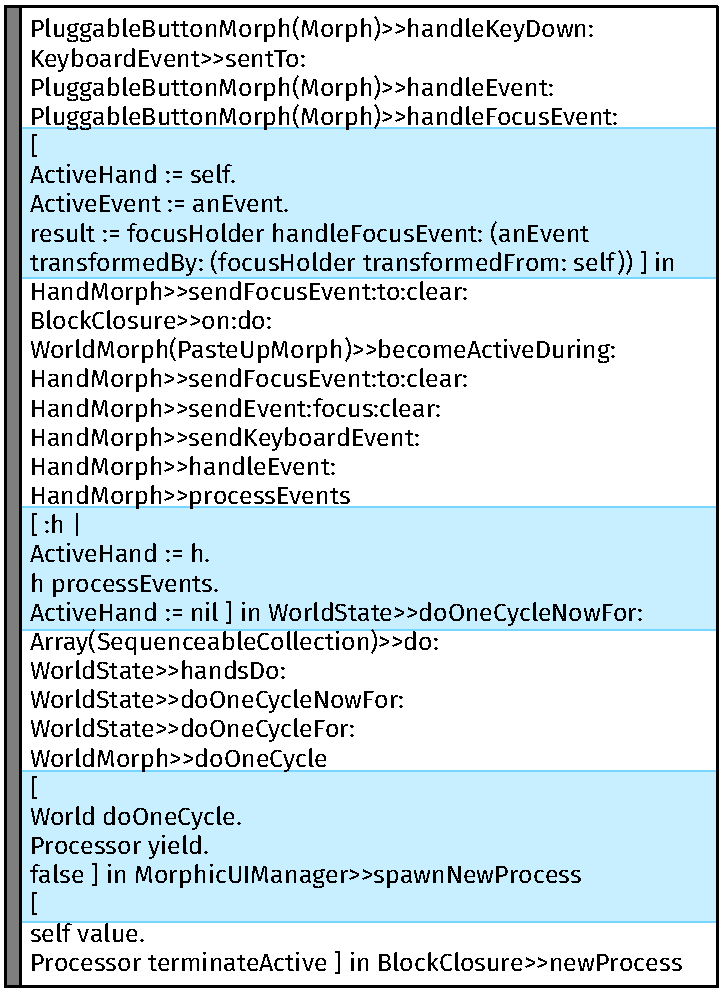
\includegraphics[width=7.3cm]{stacktraces/stacktrace}
  \caption[Example of a stack trace collected from a runtime exception]{Example of a stack trace collected from a runtime exception.
The most recent call is at the top, the oldest call is at the bottom.
The snippets of code inside blocks are highlighted in blue.}
  \label{fig:stacktrace}
\end{figure}

As we can see from the listing, the stack trace occasionally contains small snippets of code included in blocks (between square brackets, highlighted in blue).
This happens when a method executes a block.
Since in Smalltalk a block is equivalent to a closure, it represents a pluggable behavior that can change the flow of the program and, as such, it is reported into the stack trace.

Some class names are complemented with the name of a superclass between parenthesis.
This happens when the called method is not defined in the class itself, but it has been inherited from the specified superclass.
This notation maintains the link between the class involved in the exception and its superclass: It is important to keep track of this information, since the cause of an error can be rooted in the superclass chain and suggest a possible defect in the original method, as well as being a consequence of the interaction with the code of the subclass.

\subsubsection{Stack traces and dynamic typing}

An interesting property of \pha comes from its dynamic nature: the whole system is polymorphic, and polymorphism is obtained through the so-called \emph{duck typing}~\cite{Chugh2012}: every object can be used in place of other objects, as long as it is able to respond to the same messages.
This entails that---as in other dynamic programming languages---there is no static type system and, as such, no static type checking: every type error happens at runtime, resulting in a \emph{Message Not Understood} kind of exception.
This peculiarity is important when considering the nature of exceptions in \pha, because the vast majority of the exceptions is caused in this context: In our dataset an exception is thrown as a result of a message not understood in more than 72\% of the cases.
Among those cases, 68\% are generated from a message sent to \emph{UndefinedObject}.
These are the equivalent of a \emph{NullPointerException} in Java.

\begin{figure*}[ht]
\centering
  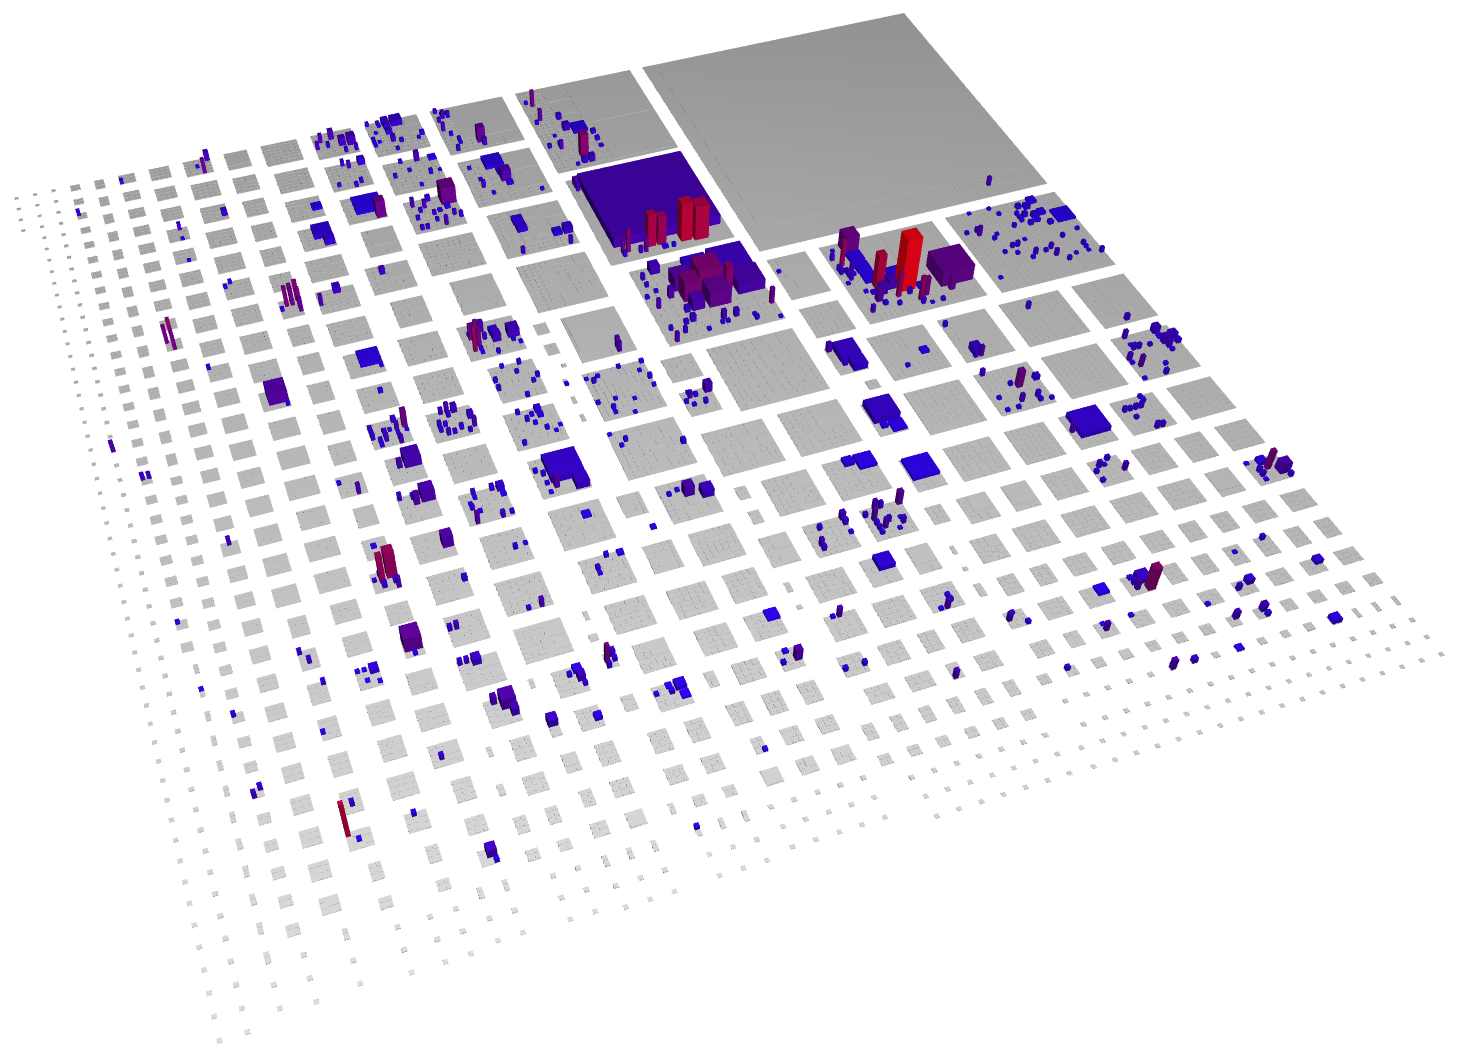
\includegraphics[width=0.9\linewidth,trim=0mm 40mm 0mm 0mm,clip]{stacktraces/StackCity_classes}
  \caption[Distribution of the stack traces on the \pha system using a city like visualization]{Distribution of the stack traces on the \pha system using a city like visualization, where each building is a class.
\pha is composed of 14,045 classes distributed among 557 packages.
We highlight the system with data from 7,532 stack traces that we collected.
The height and the color of each building is determined by the number of traces the class appears in, while classes that are not involved in an exception are collapsed and depicted in gray.
The gray squares enclosing the buildings represent the package containing the classes.}
  \label{fig:stackcity-classes}
\end{figure*}

\subsection{Interpreting Stacktraces}

The amount of information represented by type errors is ambivalent: On the one hand, it may be an effect of trivial errors from the user, such as typos, and may represent noise among the useful exceptions.
On the other hand, it contains a large amount of usage knowledge: being able to discriminate the actual failures from the occasional use errors can aid the early identification of defects and speed up debugging.
Also, what at first may look as a ``false positive'', can still be of great help in understanding how users and developers operate the system.
A recurrent and consistent misuse of a method of an API may represent a flaw in the design of the public interface of a library.
The maintainer of the library can then determine how to refactor the interface to improve the documentation.
Moreover, using further data collected after the changes, she would also be able to measure the impact of her intervention on the workflow of the developers.

Another usage example can employ data showing a frequent pattern inside core classes of the system to identify the nodes in the system that manage the largest part of the computation.
By identifying these spots, a developer could be able to prioritize her development activity and to perform targeted optimization.

So far we have considered the \emph{horizontal} dimension of stack traces, that is, we considered the information of a group of traces based on their occurrence.
However, an interesting property that we should also consider is represented by the \emph{vertical} dimension of a stack trace.
Since the order of the elements inside the trace is determined by the call sequence, the depth of a class can give us a hint of the role of the class in the computation: classes near the top of the trace provide an overview of the context where the exception originated, and can therefore be used to provide immediate feedback on the nature of the error and help debugging.
Instead, classes towards the mid part and the bottom of the trace are more related to the mechanics of the system and could be usefully aggregated to identify anomalies in the core parts of the system.

\figref{fig:stackcity-classes} shows the impact that runtime exceptions have on the \pha system, adopting a city visualization~\cite{Wett2011a}.
We aggregated the stack traces in one set of stack calls and counted the number of times a class would appear in a stack trace.
Each class is depicted as a building, where the height and the color represent how often the class is involved in an exception: the more the class appears in a stack trace, the more the color tends to red and the higher the building.
Classes that are not touched by any stack trace are depicted in gray and collapsed.
From this figure we can see how the number of classes involved in exceptions is much lower than the total number of classes in the system, therefore suggesting some hot spots in the system that could be investigated for further development activities.

\subsection{A Practical Use Case}

To be able to deal with a potentially large volume of information, we need an effective approach to classify the stack traces.
In \secref{sec:stacktraces-dataset} we present an approach based on clustering stack traces by similarity, and then stratifying horizontally the clusters using the number of members in each cluster to represent the frequency of the similar exceptions.

The most immediate advantage of using clustered stack traces is to leverage them for bug fixing.
We developed an approach to analyze the contents of a stack trace and use the mined information to retrieve bug reports from the \pha bug tracker that discuss the classes and methods in the trace.
For example, by retrieving the reports related to the trace in \figref{fig:stacktrace}, which involves key events, we can find the bug report $\#12973$, that discusses an issue related to keyboard shortcuts.
By further reading the report, we can learn about the nature of the issue, and by checking the last events we can learn about the current status of the defect.
In this case, we can see that the issue has already been resolved, a patch has been committed and is waiting to be integrated.
Thus, we can ignore the problem, knowing that it will be solved soon.
Moreover, by checking future stack traces, we are able to determine if the problem has been completely solved or if it may appear again in some particular, missed corner cases.

Overall, by being able to access bug reports related to an exception while she is experiencing it, a developer can get an overview of a problem sooner and cut the overhead time spent searching for relevant information, thus supporting a more efficient debugging process.
% Overall, having quick access to bug reports related to encountered exceptions can help to obtain an overview of the problem and improve and boost the debugging process.
In the next section we show how to match bug reports and stack traces.


\section{CrowdStacking Traces}\label{sec:stacktraces-dataset}

Stack traces are a frequent and recurrent side product of the daily workflow of developers.
Such data represent a significant amount of information that is usually not collected and thus lost.
To benefit from this data we built \slr, a tool to intercept exceptions, the corresponding generated stack traces, collect the resulting data and submit it to a central server.


\subsection{Data Collection}\label{sec:stacktraces-tool}

\slr is a plugin designed and built to integrate seamlessly into the \pha development environment.
We wanted to collect unbiased and uniform data, so we paid particular attention in building a tool that could be unobtrusive and that required minimal interaction with the user.
For this purpose, \slr is highly configurable through a dedicated settings menu, and can work in two different main modes: an \emph{interactive mode}, and a \emph{shadow mode}.

\subsubsection{Interactive Mode}
It is designed to allow the developer to keep full control of her data and decide which are the traces to submit and which ones to discard.
\figref{fig:shoreline-reporter} shows the main elements of the interactive user interface.

\begin{figure}[ht]
\centering
  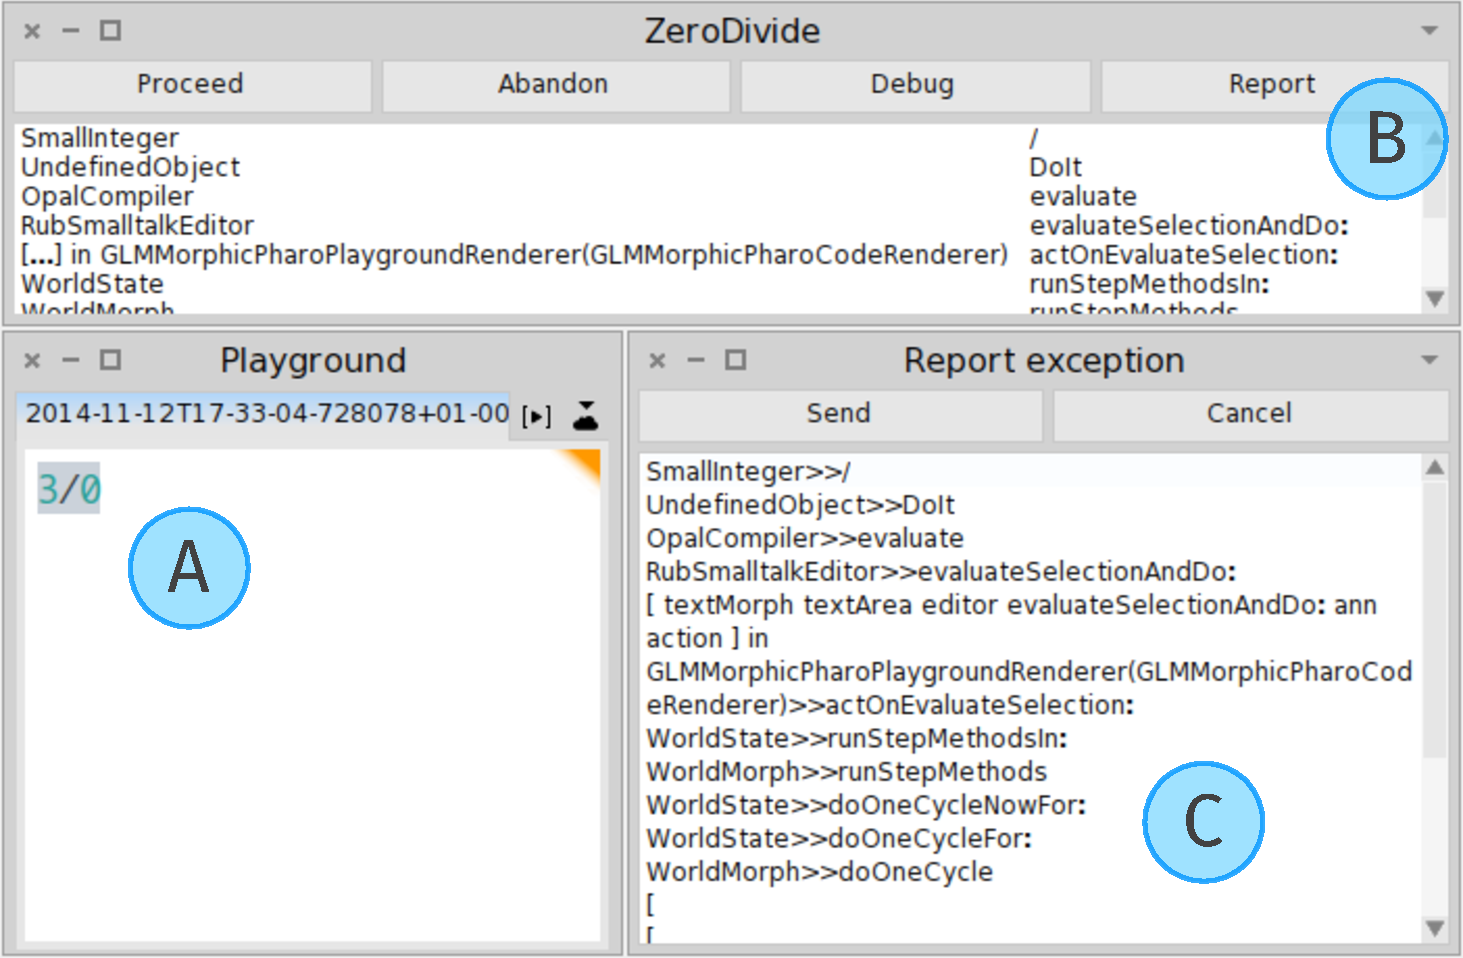
\includegraphics[width=.95\linewidth]{stacktraces/ShoreLine-Reporter.pdf}
  \caption{The interactive interface of ShoreLine Reporter}
  \label{fig:shoreline-reporter}
\centering
\end{figure}

\slr activates when the user runs code that triggers an exception \textcircled{\scriptsize A}.
The \pha IDE generally pops up a \emph{pre-debug window} \textcircled{\scriptsize B}, that illustrates a preview of the exception and the options that she can undertake.
Here \slr shows up, proposing a \emph{Report} button that allows the user to send the trace to the ShoreLine server.
If she chooses to do so, she is presented with a window \textcircled{\scriptsize C} that allows her to review the data that is being submitted to verify that it does not leak undesired information.
Once the user presses the \emph{Send} button, the reporter serializes the stack trace and submits it.

\subsubsection{Shadow Mode}
By acting on the system configuration, the user can reduce the level of interaction with the tool at the point of making it become completely transparent: She can decide to submit every stack trace without confirmation and also disable the intermediate check for the data she is sending.
In short, \slr can become completely silent and gather all the stack traces from each exception.
This is particularly important to avoid continuous prompts to the user asking for a confirmation and allow \slr to gather a significant number of stack traces without breaking the workflow of the developer.


\subsection{Data Representation}

In \pha, everything is modeled as an object.
As such, a stack trace is a complex object containing a reference to the debugger, the full context of the exception and the sequence of method calls that constitutes the trace.
However, to value privacy and to avoid our tool from being intrusive, we decided to serialize the whole stack trace as a list of strings, each one containing just the signature of methods, formatted as \textit{ClassName{>}{>}methodSelector}.
Thus, we discard all the elements that contain private data, such as the contents of instance variables.
Encoding a stack trace using strings also guarantees compatibility and portability of the collected data, even when imported from different versions of \pha.

Besides collecting the stack traces, we also added to the report additional metadata to allow a better categorization of the error.
We collect the name of the author, which is the tag she uses to sign her commits, the date of the exception and the version of the \pha build for which the exception happened.
The version of the build can be useful to analyze the evolution of the system while it is developed.
The \pha development cycle is structured in two main branches: a stable version and a development version.
In the \pha community, the development version is actively developed and constantly improved by a large number of users and developers, and exception data from developed software can provide insights about the evolution of the system over time, as well as help spotting defects as soon as they arise, ultimately reducing the time required to fix a new defect after it is introduced.

\subsection{Analysis on the Collected Data}

We collected stack traces during a time period of five months, from June to November 2014.
\tabref{tab:data-summary} shows a summary of the data we collected during that time span.

\begin{table}[ht]\small
\centering
\caption{Summary of the stack traces collected from June to November 2014}
\rowcolors{1}{tablefirstrow}{tablesecondrow}
\begin{tabular}{lr} \hline
\# of stack traces & 7,532 \\
\# of lines in all stack traces & 252,668 \\
\# of developers & 8 \\
average lines of a stack trace & 34 \\
size of the shortest stack trace & 1 \\
size of the longest stack trace & 314 \\ \hline
\end{tabular}
\label{tab:data-summary}
\end{table}

We visualized the data to highlight the parts of the \pha system that were involved in the collected exceptions: \figref{fig:stackcity-methods} shows a city visualization of the stack trace data mapped on the whole \pha system.
Using the same convention used in \figref{fig:stackcity-classes}, each building represents a class and each square enclosing a building is a package.
Each building is composed of blocks, each one representing a method.
The color of each method is determined by the number of times a method appears in a stack trace: it tends to red when the number is higher and to blue when the number is lower.
Methods, classes and packages that do not appear in a stack trace are collapsed and depicted in gray.

\begin{figure}[ht]
\centering
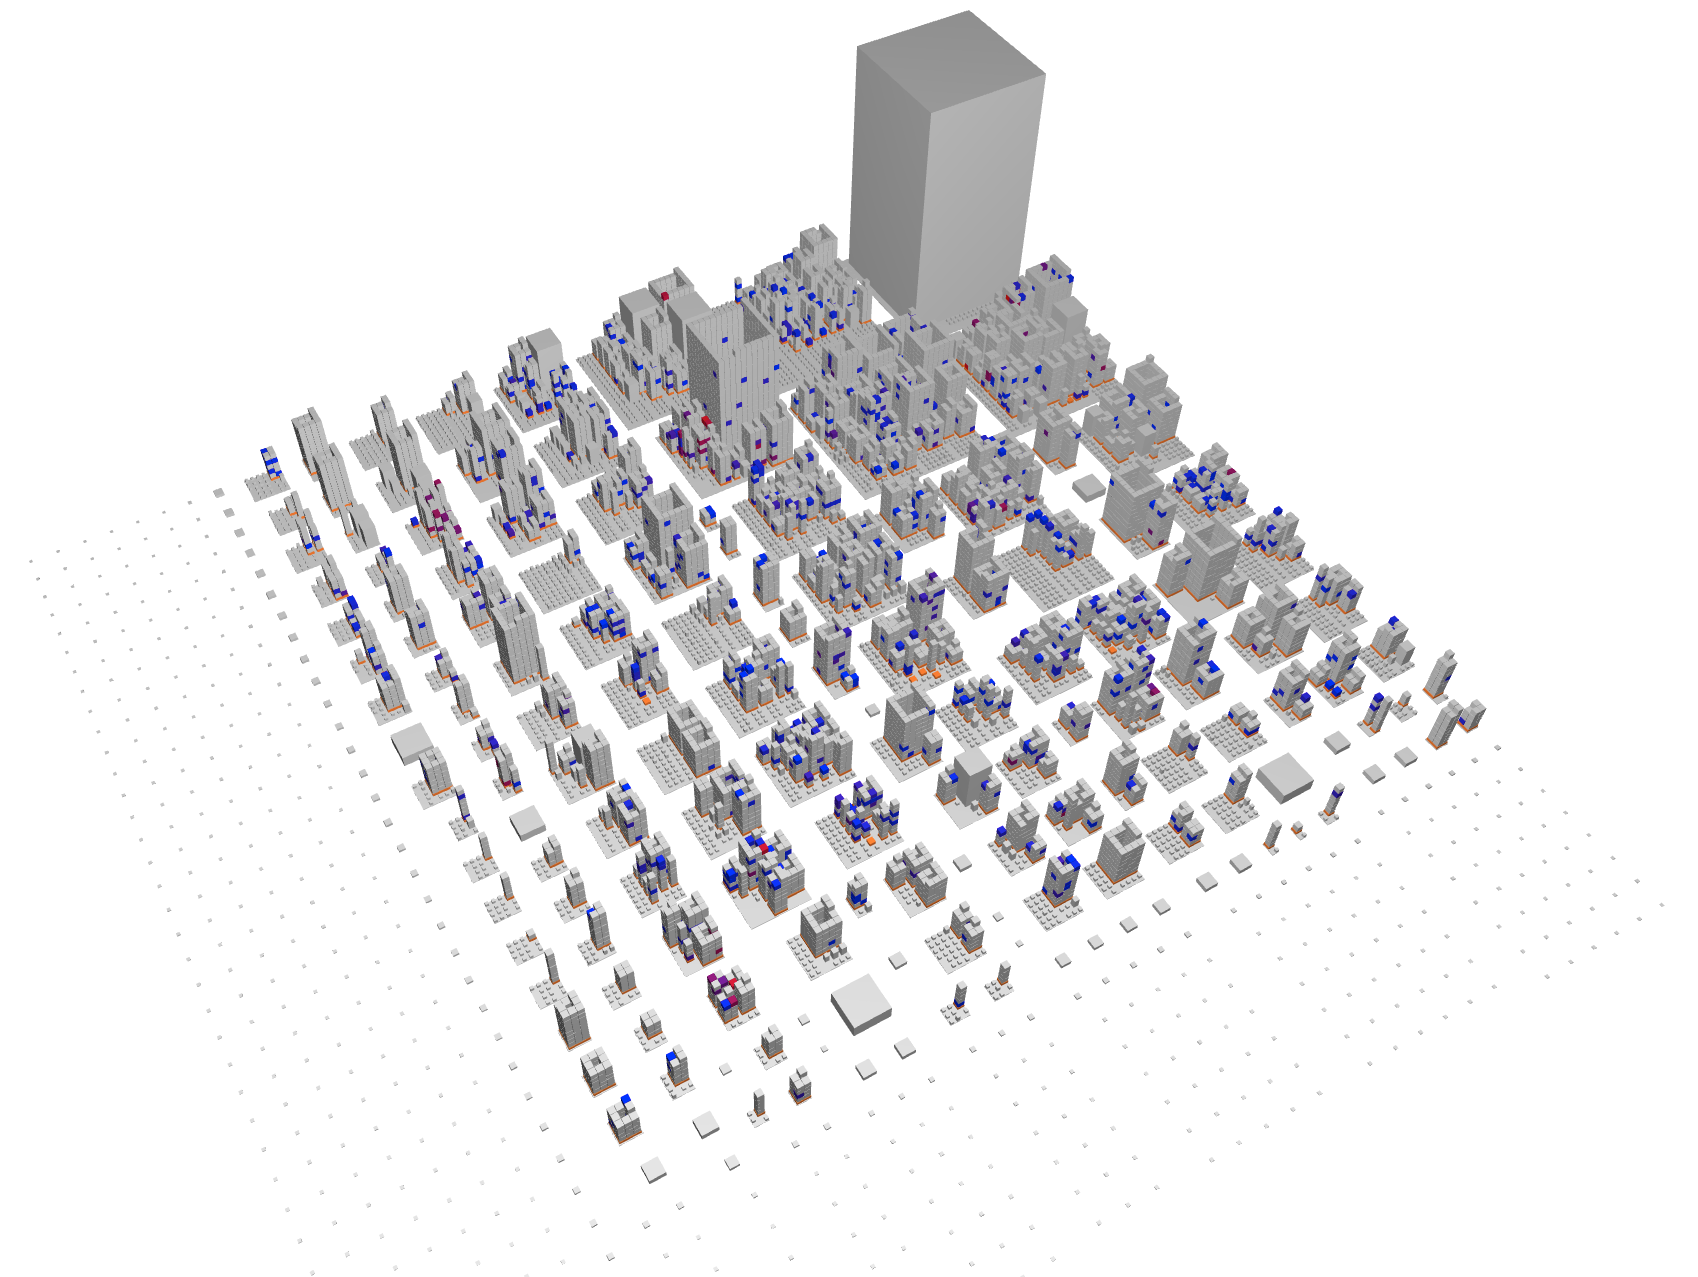
\includegraphics[width=\linewidth,trim=0mm 40mm 0mm 0mm,clip]{stacktraces/StackCity_methods}
\caption[Distribution of the stack traces on the methods of \pha using a city like visualization]{Distribution of the stack traces on the methods of \pha using a city like visualization, where each building is a class composed by blocks representing methods.
All the classes contain 112,558 methods, the color of each building is determined by the number of traces the class appears in, while the packages, classes and methods that are not involved in an exception are collapsed and depicted in gray.}
  \label{fig:stackcity-methods}
\end{figure}

The figure suggests that only a small part of the system is actually involved in the collected exceptions, and the vast majority of methods and classes is not impacted by them.
By knowing these methods that work as entry points to the classes, a developer can view the impact that each class and method have in case of failures: This information can be useful in having a first prioritization to decide which methods she has to inspect first to search for a bug.

\begin{table}[t]\small
\centering
\caption{The 10 most called methods in the collected stack traces.}
\rowcolors{1}{tablefirstrow}{tablesecondrow}
\begin{tabular}{lr}
\textbf{Class{>}{>}Method} & \textbf{Occurrences} \\ \hline
BlockClosure{>}{>}on:do: & 9,265 \\
UndefinedObject{>}{>}doesNotUnderstand: & 8,549 \\
BlockClosure{>}{>}cull:cull: & 6,268 \\
Message{>}{>}sentTo: & 4,980 \\
PragmaMenuBuilder{>}{>}collectRegistrations & 4,776 \\
WorldState>>doOneCycleNowFor: & 4,714 \\
BlockClosure>>on:fork: & 4,554 \\
Array>>do: & 4,497 \\
BlockClosure>>ensure: & 4,495 \\
BlockClosure>>cull: & 3,642 \\
%OrderedCollection>>do: & 3,541 \\
%AnnouncementSubscription>>deliver: & 3,490 \\
%BlockClosure>>newProcess & 3,352 \\
%PragmaMenuBuilder>>currentRoot:while: & 3,184 \\
%HandMorph>>sendFocusEvent:to:clear: & 3,078 \\
%WorldState>>doOneCycleFor: & 2,869 \\
%WorldMorph>>doOneCycle & 2,865 \\
%MorphicUIManager>>spawnNewProcess & 2,861 \\
%BlockClosure>>cull:cull:cull: & 2,428 \\
%FormCanvas>>roundCornersOf:during: & 2,017
\hline
\end{tabular}
\label{tab:methods-count}
\end{table}
\tabref{tab:methods-count} shows a summary of the most active methods in all the stack traces.
As expected, the most recurrent exceptions are related to some core elements of the language: \textit{BlockClosure} is a core element used when passing code as argument, while \textit{UndefinedObject>>doesNotUnderstand:} and \textit{Message>>sentTo:} are part of the message sending infrastructure that is the foundation of Smalltalk.
%The former is equivalent to a \textit{NullPointerException} in Java.
Despite being expected, the fact that the most common exceptions involve the dynamic nature of the language shows how the freedom provided by the absence of static type checking comes with the price of incurring in runtime exceptions even for experienced programmers.

Once verified that the most recurring exceptions are caused by common usage patterns of the language, we can consider these elements as outliers for the specific purpose of this work: The information they carry can still be useful in identifying other issues like API usage problems, but it is likely negligible to be connected to bug reports.
Moreover, methods that appear in very few stack traces are also outliers, since there is an intrinsic lack of confidence that they can be significant to represent any pattern in the system.

\subsection{Extracting Information}

We saw that many stack traces are channelled mainly through few crucial points in the system.
To inspect whether it was possible to group them, we applied a clustering approach to detect the stack traces that could be generated by similar errors.
Clustering stack traces can give us the advantage of reducing the number of elements that we have to inspect to determine whether a given error is caused by a defect, by bad usage or simply by a behavior of the developer (\eg in the case of Test Driven Development).
Inspired by a technique used in information retrieval, we mapped our stack traces to a \textit{vector space model}~\cite{salt1975}.
A vector space model is a data structure to index documents and perform efficient comparisons between each document.
In information retrieval it is built by splitting a document in a sequence of terms, and turning the document in a vector counting the number of occurrences of each word in the document.
We build our vector space model by building a vector for each stack trace: we use the pair \textit{ClassName{>}{>}MethodName} to identify the features (the terms) of the vector.
We collected all the features in a dictionary and used it to build each vector, where the components of the vector contain the number of times that a method invocation appears in the stack trace.

\newpage
For example, consider the two stack traces containing the method calls:
\begin{center}\small
  \begin{tabular}{lll}

    \begin{tabular}{l}
      \textbf{Trace 1} \\ \hline
      UndefinedObject{>}{>}DoIt \\
      BlockClosure{>}{>}valueAfterWaiting: \\
      BlockClosure{>}{>}newProcess \\
    \end{tabular}

    & &

    \begin{tabular}{l}
      \textbf{Trace 2} \\ \hline
      TabManager{>}{>}setTabContentFrom: \\
      Tab{>}{>}retrieveMorph: \\
      BlockClosure{>}{>}newProcess \\
    \end{tabular}

  \end{tabular}
\end{center}

\pagebreak[2]

We collect all the terms and build a dictionary composed of the features:
\begin{center}\small
\begin{tabular}{l}
\textbf{Dictionary} \\
BlockClosure{>}{>}newProcess \\
BlockClosure{>}{>}valueAfterWaiting: \\
Tab{>}{>}retrieveMorph: \\
TabManager{>}{>}setTabContentFrom: \\
UndefinedObject{>}{>}DoIt
\end{tabular}
\end{center}


Using the dictionary we can then build the vectors for the two stack traces:

\begin{center} % ok
\begin{tabular}{p{2cm}r}
\textbf{Trace 1} & $\left<1,1,0,0,1\right>$ \\
\textbf{Trace 2} & $\left<1,0,1,1,0\right>$
\end{tabular}
\end{center}

Once we have our vector space model, we can define the distance between each stack trace.
For this, we need to define a similarity measure, that indicates how two stack traces are different according to our metrics.
Having a vector space model allows us to calculate distances by means of the \emph{cosine similarity}, which for two vectors can be calculated from the definition of the Euclidean dot product, that is:

\begin{displaymath}
    \cos\theta=\frac{A \cdot B}{\|A\|\|B\|}
\end{displaymath}

In the case of documents, where the vectors have all positive components, the similarity ranges from 0 to 1.
In the previous example, the distance for the two vectors representing Trace 1 and Trace 2 is 0.58.
Using the cosine similarity we calculated the first nearest neighbor for each stack trace.
With this data we were able to construct a visualization to understand the topology of the stack traces in our vector space model.

\figref{fig:eva-clusters} shows a force graph where each dot is a stack trace and every edge represents the connection between each trace and its nearest neighbor.

\begin{figure}[h!t]
\centering
  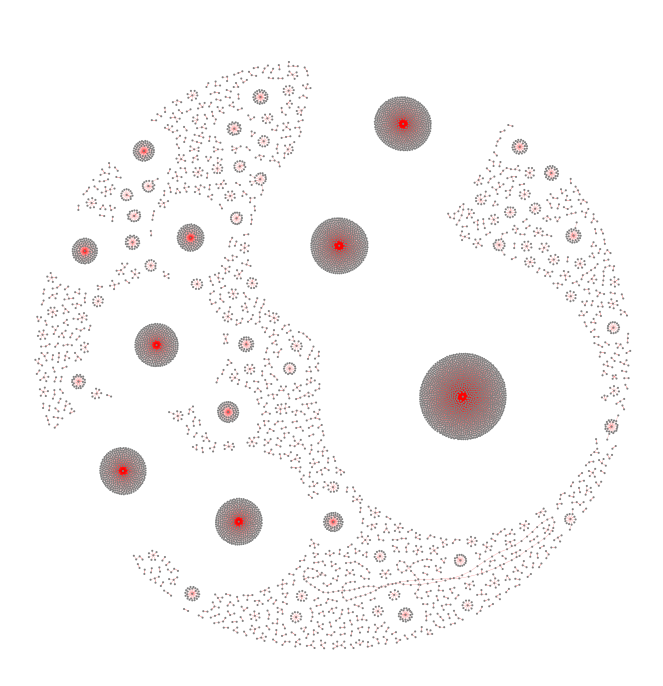
\includegraphics[width=\linewidth]{stacktraces/TraceClusters}
  \caption[Force graph representing the stack traces and their neighbors]{Force graph representing the stack traces and their neighbors.
  Each dot is a trace, each edge connects a stack trace with its nearest neighbor.}
  \label{fig:eva-clusters}
\end{figure}

The figure shows evidence that there are groups of related stack traces, gathered around a pivotal point.
In particular, few large groups gather the majority of stack traces, and the remaining form smaller groups.
To represent each cluster, we chose the \emph{medoids}~\cite{Kauf1987}.
A medoid is the element of the dataset that is nearest to the centroid of the cluster.
The advantage of using medoids instead of centroids is that they are an element of the dataset, and thus they represent a stack trace that actually occurred.
Moreover, centroids tend to be much more sparse that medoids, thus being more suitable for efficient computation of operations between vectors.
We considered the medoids as \emph{archetypes}, that represent the summary of each cluster.
The number of incoming edges represents the measure of the popularity of the archetype and, as such, of the whole group.

\begin{table}[ht]\small
\centering
\caption{Summary of the most popular stack traces, with the popularity metrics.}
\rowcolors{1}{tablefirstrow}{tablesecondrow}
\begin{tabular}{lr}
\rowcolor{tableheader}\textbf{Archetype (first line)} & \textbf{Popularity} \\ \hline
UndefinedObject>>doesNotUnderstand: & 1,585 \\
UndefinedObject>>doesNotUnderstand: & 647 \\
UndefinedObject>>DoIt & 619 \\
UndefinedObject>>doesNotUnderstand: & 428 \\
UndefinedObject>>doesNotUnderstand: & 427 \\
RGFactory>>doesNotUnderstand: & 363 \\
BlockClosure>>doesNotUnderstand: & 127 \\
UndefinedObject>>doesNotUnderstand: & 111 \\
SystemDictionary>>errorKeyNotFound: & 71 \\
MouseWheelEvent>>doesNotUnderstand: & 69 \\
UndefinedObject>>doesNotUnderstand: & 57 \\
NBGLFrameBuffer>>error: & 41 \\
RTDraggable>>initializeElement: & 29 \\
UndefinedObject>>DoIt & 29 \\
UndefinedObject>>DoIt & 28 \\
%R3KeyControl>>initElementForMac: & 28 \\
%R3MouseControl>>initElement: & 26 \\
%UndefinedObject>>doesNotUnderstand: & 26 \\
%SmalllintManifestChecker>>runRules:onPackage:withoutTestCase: & 24 \\
%UndefinedObject>>doesNotUnderstand: & 24 \\
%UndefinedObject>>DoIt & 23 \\
%PluggableButtonMorph>>handleKeyDown: & 23 \\
%SmallInteger>>/ & 18 \\
\hline
\end{tabular}
%\caption{Summary of the most popular stack traces, with the popularity metrics.}
\label{tab:popularity}
\end{table}

From \tabref{tab:popularity} we can see that the largest groups of stack traces are generated by exceptions related to the dynamic nature of the language, and as such probably caused by the style of programming of the developer.
We still believe that this information can provide deep knowledge over the status of the system, but we think that their analysis represents a different set of problems that could be tackled with statistical analysis of big volume of stack traces during the evolution of the system.
Therefore, at this stage we removed the most popular groups, and focused our inspection on the traces positioned in the central part of the ranking.
We used these samples to determine a possible correlation with existing defects.

We mined the \pha bug tracker to collect the bug reports produced during the development of the platform.
To focus our research on actual and relevant problems, but without risk of losing valid examples, we considered the reports opened between January and November 2014.

We extracted 1,910 bug reports, with 17,747 different events, including comments, patches and changes of status.
During this period, 1,591 reports have been closed or are waiting for integration, and 319 are still active.

We then extracted from each archetype of stack trace a list of methods invocation.
We used this list to search through the data extracted from the bug tracker using a full text search of the pair \emph{ClassName{>}{>}MethodName} into the contents of each comment that compose a bug report.
After this operation, we obtained a list of the bug reports that are associated to each method invocation.
Not every bug report can have the same relation with the stack trace, therefore we applied a heuristic approach to define a ranking to sort the reports in order of likelihood of relevance.

We discussed earlier how the lines of a stack trace that are closer to the top are more likely to be related to the current error, while the lines closer to the bottom are more likely to touch the core parts of the system and thus more generic.
We leveraged this principle to give a higher ranking to the reports retrieved using lines closer to the top of the stack trace and lower ranking to those retrieved by lines close to the bottom.
In the scenario of a context-aware tool that suggests interesting reports to developers while they encounter exceptions, we observed that the interesting bug reports are likely to be in the first three positions.
After these, the link between a stack trace and the information in a bug report quickly becomes too general and likely related to internal mechanics of the system.



\section{Preliminary Results}\label{sec:stacktraces-evaluation}

% Numbers of topic considered has to be justified
We obtained a list of bug reports connected to each archetype stack trace, that we called \emph{topic}.
We performed a qualitative analysis on the topics to determine if the retrieved reports could actually provide valuable information about the nature of the exception.
We removed from the list the topics triggered by a \emph{doesNotUnderstand:} and \emph{UndefinedObject}, because they are mostly generic and less likely to contain specific bug reports in the tracker.
After the filtering, we reduced the list to 629 elements.
We then eliminated the elements with the lowest popularity, to exclude the groups that had not enough components to be significant.
We set the threshold to be the 0.5\% of the maximum popularity, which gave us a list of 23 elements, with a significantly diverse popularity ranging from 1,585 to 9.

We manually inspected the bug reports related to each topic, to determine if they contained information relevant to original exception that would therefore be useful in supporting the development and debugging process.
Of the 23 topics, 15 of them had no bug reports connected in the top of the trace and had only reports in the bottom, related to generic mechanics of the system, unrelated to the specific exception.

The fact that some stack traces had no connected bug reports could have different meaning, and may carry interesting information that may be used in the debugging activity:

\begin{enumerate}%[(1)]

\item It may represent an exception that occurs in code that is specific to the project of a developer and therefore not discussed in the system bug tracker;

\item It may be due to a misuse of an API that leads to type errors;

\item It may be caused by a new defect, not yet reported.

\end{enumerate}

Each of the three cases can represent an interesting scenario that can be addressed with a different practical action.

In case (1) the information about runtime error of a developer's code can be of interest for the developer itself and, if collected for further usage during debugging, it can be used to signal possible defects in the code and prioritize the classes and methods to inspect.

Case (2) can take place when many developers use the same API in an incorrect way.
Such a case may suggest an area of code or a class interface that requires refactoring.

Case (3) is the most interesting for the developers of the system: It means that the system is raising a lot of exceptions in an area of code that is not known yet for having unexpected behaviors.
This could---by definition---represent a new defect, not yet known to the community, or not precisely defined.
In this case, grouping the stack traces and highlighting them as a problem to investigate, may provide a valuable support for the community, for example by proposing to automatically open a new bug report containing the collected data to start the debugging activity when the popularity of the group reaches a critical mass, and help to severely cut down the latency between the introduction of a defect and its resolution.

For the remaining 8 stack traces we found related bug reports in the bug tracker.
After assigning every report a priority depending on the distance of the top of the stack, we inspected them in order of priority.
We observed that, given the structure of the stack trace, only the bug reports in the first two or three lines of the trace are relevant to define the context of the precise problem: the trace of calls then quickly dives into the system core classes becoming thus too generic to pertain to specific scenarios.
We found the information of the reports to be relevant to the debugging activity, or to get information on the status of the malfunction: Either the identified reports were addressing the specific issue raised by the stack trace, or were not depicting the same specific context of the exception, but still discussing a related problem.

We now present two example bug reports and show how they are relevant in understanding an exception during development.


\clearpage

\begin{figure}[!ht]
\centering
  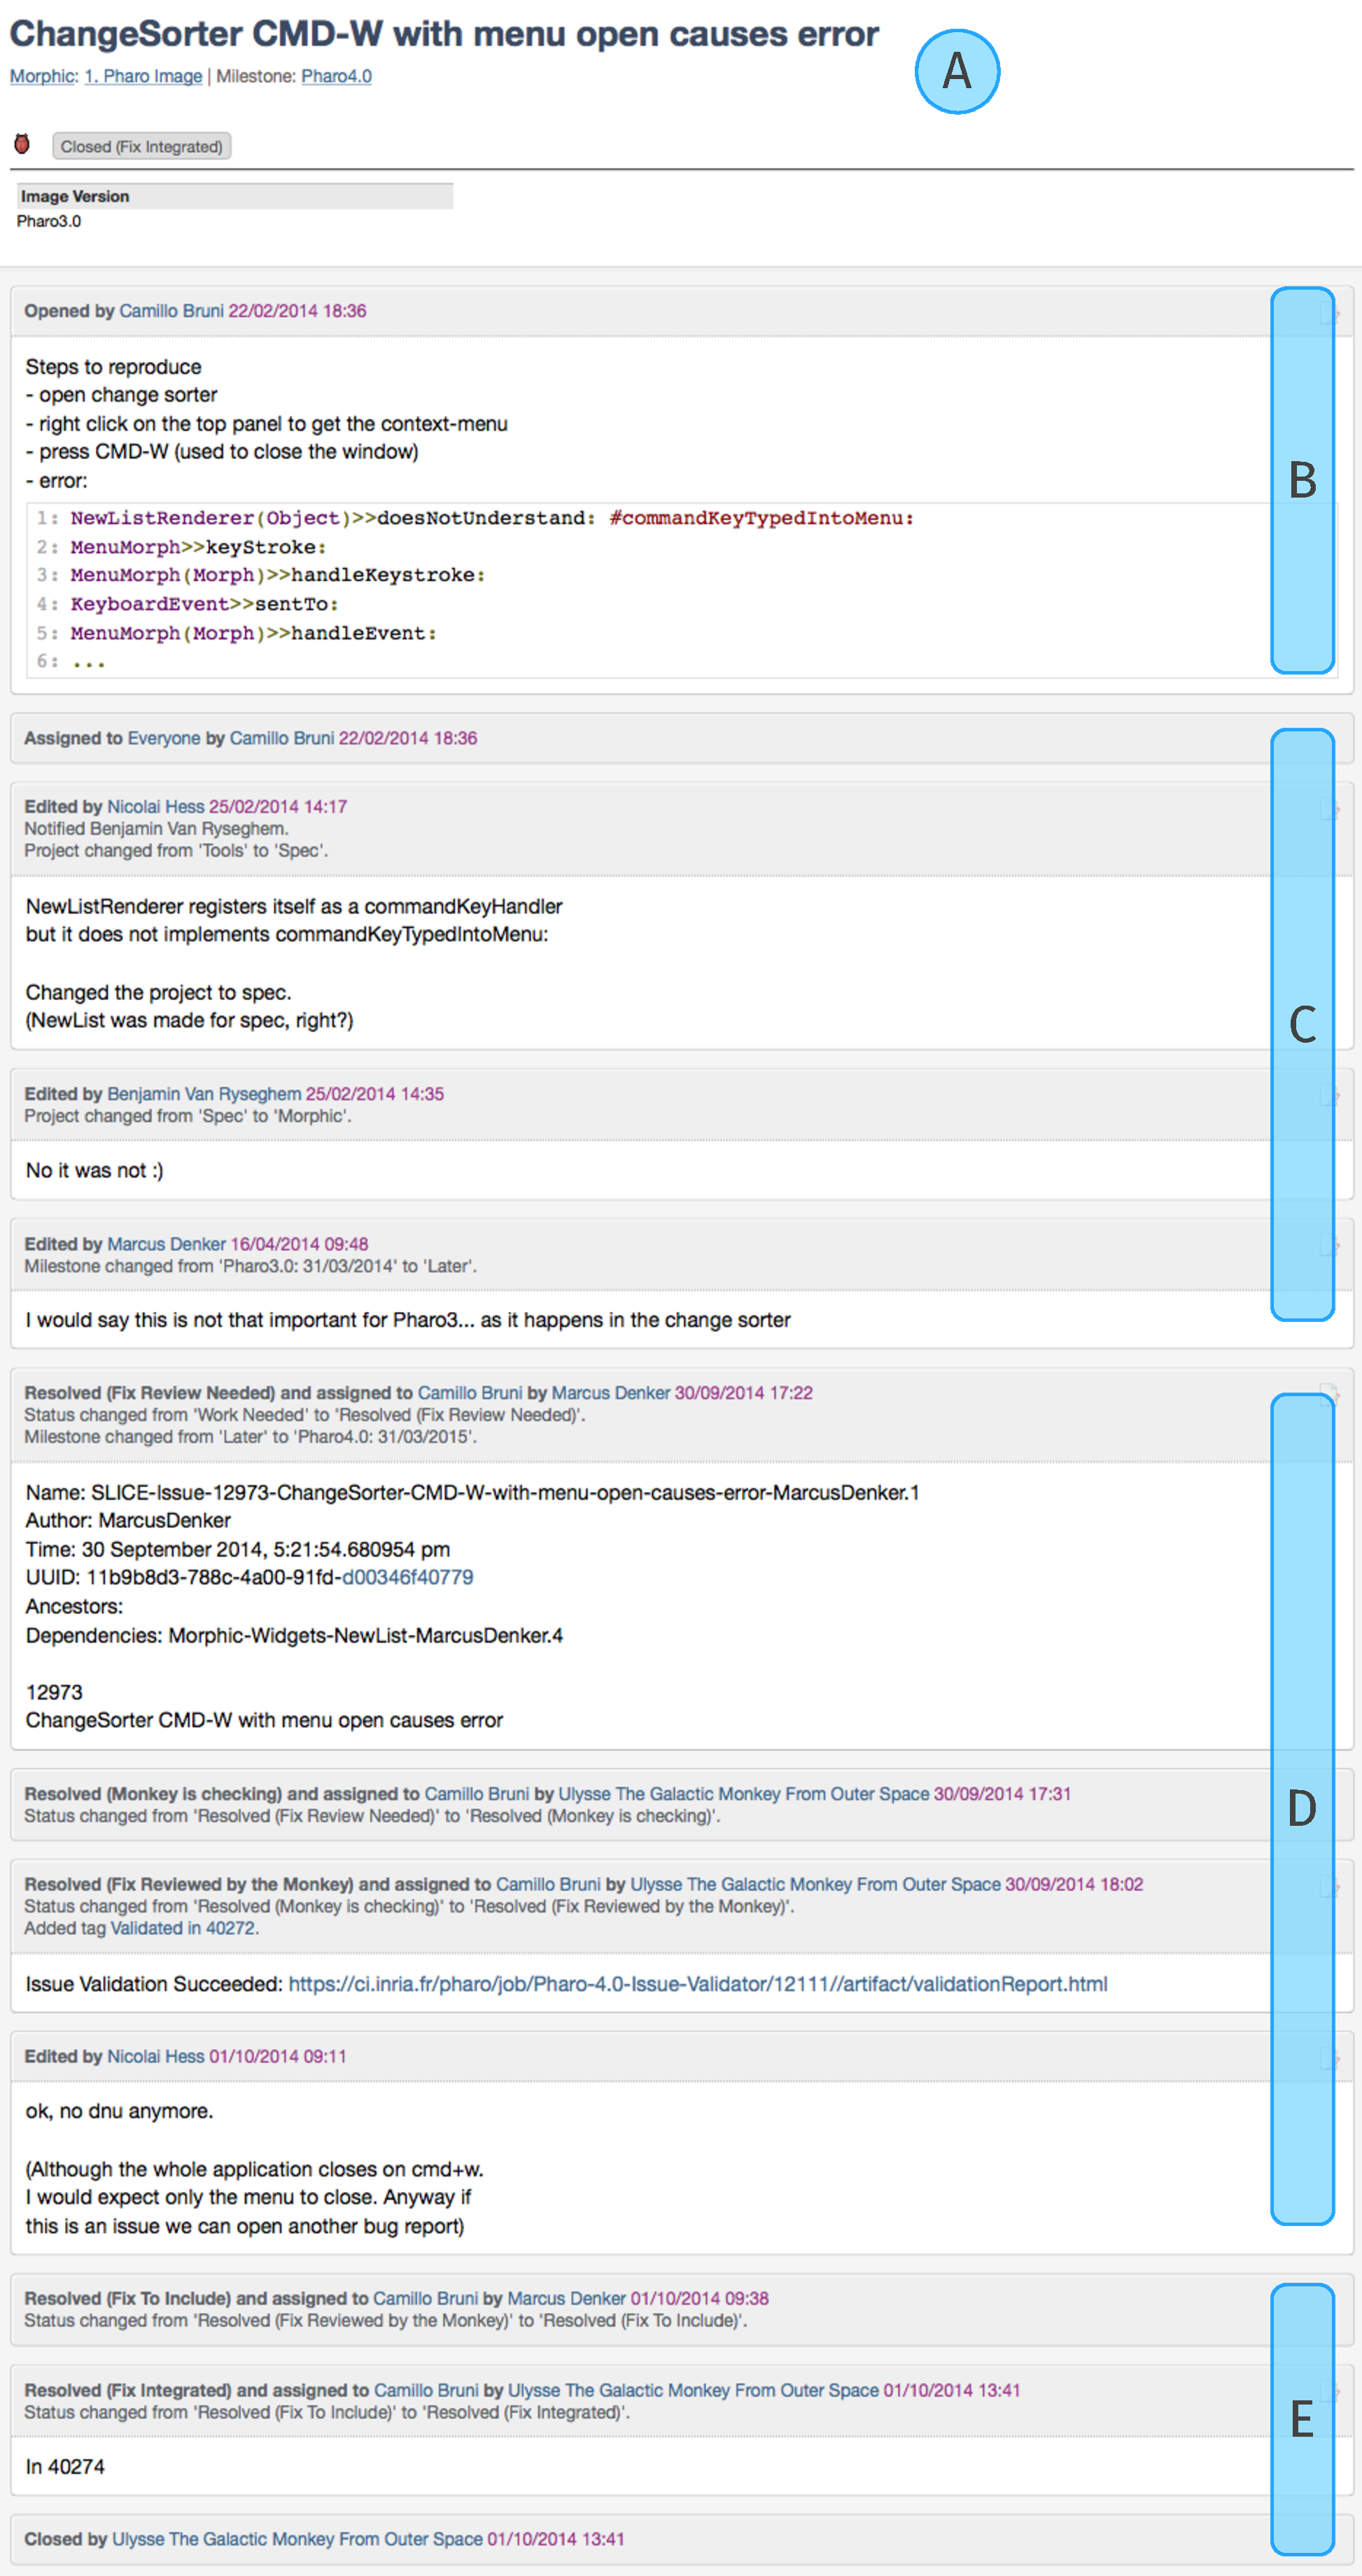
\includegraphics[height=.87\textheight]{stacktraces/Report-12973.pdf}
  \caption[The bug report 12973]{The bug report 12973, related to the stack trace depicted in \figref{fig:stacktrace}.
We can see the metadata (A), the initial description that opened the bug report (B), the discussion that followed (C), the submission of a slice and its validation (D), and the bug resolution (E).}
  \label{fig:report}
\end{figure}

\subsubsection{Example 1}

In \secref{sec:stacktraces-nature} we already presented the stack trace shown in \figref{fig:stacktrace}.
The example is particularly interesting because it shows a practical use case for a user or a developer that encounters the exception while she is writing code.
\figref{fig:report} shows the bug report retrieved for this stack trace.
As the report shows, there is a known error caused by a defect in the system, and the community is already working to address it.
In particular, since the stack trace that we considered was generated on date 7/7/2014, the user encountered the problem before its resolution and, at the time, the report was stuck in a low priority status.
This information could have been exploited by a developer to report more precise information or to ask for an increase of the priority for a quicker defect resolution, while a user encountering the exception could know that there is work in progress, or if there is an estimated time to have an updated and fixed version.

By continuing to read the report, we can see that the problem has been further investigated, and that a \emph{slice} (a piece of submitted code, that in \pha works in a similar way of a patch) has been proposed and is being tested on the continuous integration server of the project.
Finally we can see that the report was closed, the fix was accepted and it is waiting to be integrated in a later version.

Other than simply useful, this information can improve awareness among developers.
For example, by depicting a lively and active community, it may disseminate and reward the contributions targeted at improving the general quality of the whole system.


\subsubsection{Example 2} Another example is represented by the stack trace starting with:

\begin{center}\small
\begin{tabular}{l}
SmalllintManifestChecker{>}{>}runRules:onPackage:withoutTestCase: \\
RBPackageEnvironment{>}{>}classesDo: \\
Set{>}{>}do: \\
RBPackageEnvironment{>}{>}classesDo: \\
Set{>}{>}do: \\
RBPackageEnvironment{>}{>}classesDo: \\
SmalllintManifestChecker{>}{>}runRules:onPackage:withoutTestCase: \\
CriticBrowser{>}{>}reapplyRule:
%Set>>do:
%CriticBrowser>>reapplyRule:
%CriticBrowser>>reapplyThisRule
%Array>>do:
%CriticBrowser>>reapplyThisRule
%CriticBrowser>>menu:shifted:
\end{tabular}
\end{center}


The lines containing \emph{CriticBrowser{>}{>}reapplyRule:} are related to bug report 14230.
On closer inspection we can see that the bug report contains only three comments, but the last one points to report 110473, where a long discussion (40 comments) is ongoing regarding the relation of the method in the stack trace and the application of rules for the CriticBrowser.
At the end of the discussion the report gets closed, but as a result of the fix, another bug report is issued to address further weird behavior of the CodeCriticBrowser.
To add even more correlation to the trace and the report, we noticed that the author of the stack trace is active in the discussion of the report, and actively contributed to its resolution.
This reinforces our belief that providing a bug report context when a user encounters an exception can provide great value in debugging software.




\section{Discussion}\label{sec:stacktraces-discussion}

We discussed our approach and its preliminary results in investigating the stack trace data that we collected.
We now take a critical stance towards our approach, discussing the data, the approach itself and the actual impact that it can have on a development community.


\subsection{The Data}

During this experiment we collected novel data generated from actual daily development activity.
The biggest threat that we see in our work is given by the nature of our dataset.
Despite having a considerable amount of stack traces, the fact that they were produced by just eight developers may introduce hidden patterns caused by the specific style of programming of each developer, or by the codebase the developers were working on during the experiment.
This could lead to a latent bias in our results, that may prove to be too tailored for our users.
We are expanding the number of developers using \slr, and we will therefore be able to verify the generality and scalability of our approach.

Despite this threat, we believe that the data we collected contains valuable and unexploited information, that can lead to the discovery of hidden patterns in developers' activity.
Analyzing this information can produce knowledge that can be helpful in supporting the developers during the bug fixing activities, and can support the work of the community.


\subsection{The Approach}

We designed our approach to find immediate use of the stack traces, and confirm that the data we collected contained information that was both significant and interpretable.
However, there are many improvements that can be done to refine the way that we process stack traces  and link them with bug reports.

One can argue that the use of clustering is not really necessary in finding a correlation between a stack trace and a report, and that a simple direct search of the elements of a stack trace is sufficient to find the relevant matches.
However, we believe that the use of clustering carries some advantages that can be valuable in building a tool to provide feedback on actual data.


\subsubsection{Generalization}
First of all, the use of clustering allows to identify, group and ``average'' similar stack traces, having the effect of making the whole process more robust and noise resistant by considering only the most popular stack trace in the group.
In this way, even changes in the system that would generate different, but still similar stack traces would have no immediate negative impact in the search result.


\subsubsection{Scalability}
Even more important, the use of clustering brings the crucial advantage of drastically reducing the size of the problem.
While this is not an impossible problem to overcome with the size of the dataset that we considered, in a real world scenario with thousands of developer constantly providing stack traces from errors, the volume of the data would quickly become impossible to process.
As such, building clusters that can be used as index and provide a quick lookup for the existing categories of stack traces is a necessary step in building a tool that provides real-time feedback to the user in an acceptable time.


\subsubsection{Metrics}
The final advantage of building clusters is that it eases further analysis on the dataset.
Clustering provides an immediate measure of the popularity of the cluster, it can help in profiling the types of errors on the system during time and ease further investigation on specific groups of stack traces, allowing deeper inspection of other unexpected behaviors on the system, such as the distribution of Message Not Understood or  the distribution of the invoked classes and methods.
To develop this approach, we used a very simple, yet effective clustering method based on the connected components of the graph formed by the nearest neighbor.
Despite its simplicity, this method already provided useful results in identifying the main groups of stack traces in the dataset, as shown in \figref{fig:eva-clusters}.
The approach can be further refined with more specific algorithms, such as k-means~\cite{MacQ1967} or k-medoids~\cite{Kauf1987,Park2009}, which could provide more precise results.
However, the cost for such improvement could be represented by a drop of performance, since these algorithms are computationally expensive.
Therefore, the nearest-neighbor clustering  represents a good tradeoff between results and efficiency.
Also, the problem of a clustering algorithm such as k-means, is that it requires to determine \emph{a priori} the number of clusters to separate our dataset, but in the context of stack traces this information is indeed impossible from the beginning, and it can invalidate the notion of similarity, degrading the approach.
Instead, our approach allows a to define a partition without previous knowledge, and that can be easily an quickly adapted as the number of instances increases, and different classes of exceptions and stack traces are discovered.


\subsection{Applicability of the Method}

We think that the ability to immediately link stack traces to bug reports can be effectively exploited to provide on-line help to a developer.
We foresee additional benefits that require additional investigation and tool support.
Our approach provides quick evidence of the problems in a system and helps finding the immediate context of the error: Therefore, it can be exploited to speed the debugging process, or it can provide information on the current status of a bug in the system.
Moreover, since the information presented to the developer depends on the context she is working on, it may also work as additional documentation, and support the understanding of some parts of the code which are poorly documented.

Besides the pragmatic aspects of assisting developers, we think that having a way to access live information on the status of the system may result in a more integrated and open development process.
A normal user can be reassured by knowing that the core development team is already dealing with a problem, while other developers may be encouraged to step in and help the resolution of the defect, either by providing additional information or by actually start working on the defect.
In an open source project, this set of conditions could bolster the interactions among the community members, focus the attention to current problems and reinforce the whole community.


\subsection{Next Steps}

We see this work as first step towards a new way of dealing with information from error contexts.
Current debugging workflows include a number of time consuming activities that could be automated, to reduce the time spent on fixing problems, speed up the development, and foster the improvement of the software project.
The approach that we presented in this chapter is only one of the many possible ways that we see possible to adopt in employing this data: leveraging this information can lead to a number of tools that can deeply impact the way communities and developers deal with debugging.
\begin{itemize}%[$\circ$]
\item\textit{Context aware debugging:} as we suggested during the chapter, we want to extend \slr to propose the possible bug reports to the developer whenever he triggers an exception, to provide a quicker access to the information needed to deal with the problem.

\item\textit{Bug triaging:} Having access to stack trace information can help identifying the types of defects that caused an exception, thus easing the process of triaging the bug~\cite{Anvi2006a}.
Also, we can use the data submitted by each user to create and update profiles of the developers and determine their area of expertise in a quick and reliable way.

\end{itemize}

There still is a significant amount of data that we did not consider during our analysis.
The information regarding the dynamic nature of the language can still be exploited to get insights on the internals of the system.

\begin{itemize}%[$\circ$]

\item\textit{System core exceptions:} We mainly focused on the top part of the trace, because it contains the part of information closer to the user.
The bottom of the stack, which involves the deeper parts of the system, can be used to find bugs hidden in the core classes of the system.

\item\textit{Stack trace patterns:} We saw from \figref{fig:stackcity-classes} and \figref{fig:stackcity-methods} that many stack traces actually touch only a small part of the system.
This is an interesting behavior that we want to investigate further, by looking for patterns in the call stack and detect how to deal with ``hot areas'' of the system.

\item\textit{Optimization:} Knowing the main areas of the system that are executed during an exception can also show the frequency of execution during the daily activity of the users.
This information can be combined with code profiling techniques to determine where and how to perform optimizations on the existing code, and improve execution performances.
\end{itemize}

We envision a future where debugging, but also development activities are supported by means of context-aware tools that use automatically extracted information produced by a whole development community, to aid the tasks of developers and support debugging, with the support of the whole community.

% \section{Related Work}\label{sec:stacktraces-related}
%
% Bug fixing is well known to be a tedious activity, and identifying the source of a problem---even with a bug report---represents a non trivial task.
% Zimmermann \etal showed that the bug reports containing stack traces improve the general quality of the report, and result in a faster resolution of the report~\cite{Zimm2010a}.
% Schr\"oter \etal provided empirical evidence analyzing the Eclipse project that the use of stack traces in defect resolution provides value in the debugging activity, and suggested that software projects should provide means to include them in defect reporting~\cite{Schr2010a}.
%
% The idea of collecting runtime exceptions to analyze software errors has been adopted by different authors in different contexts.
% Glerum \etal used an automated approach to collect errors generated and submitted by WER, the \emph{Windows Error Reporting} tool.
% They analyzed data collected from users of Microsoft's operating systems worldwide: In their approach approach they grouped the reports into buckets by looking for specific properties of the trace, and used this information to prioritize debugging and build a knowledge base where system administrators could check common problems of the system~\cite{Glerum2009}.
% Inspired by this work, Han Shi~\etal applied the same principle to performance debugging~\cite{Han2012}: They proposed an approach called StackMine, designed to detect and report highly impacting performance bugs and address defects that cause long delays in the user experience.
% We believe that a similar approach to the one that they applied to an operating system, can be a valuable support for developers in building a programming environment.
% Mozilla adopts a similar approach to collect stack traces and runtime execution for debugging purposes~\cite{McLa2004}.
%
% The information of stack traces contained in bug reports represents a valuable support in debugging: as such, many researchers devised different methods to aid bug fixing and management of reports using stack traces.
% These works provided evidence that stack traces are a useful tool and a precious source of information~\cite{Davie2013,Wang2013,Brod2005,Weis2007a}: they provide precise information that are generally more reliable and useful than the descriptions produced by the submitter of the reports~\cite{Ko2006}.
%
% Brodie \etal proposed an automated approach to group similar bug reports using stack trace~\cite{Brod2005}
%
% Moreno \etal applied Text Retrieval techniques to compute similarity between bug reports using the stack traces contained in the report description, focusing on reducing the overhead to analyze large amounts of data~\cite{Moreno2014}.
% Again, this was done in a localized post mortem way.
%
% Managing bug reports is expensive and represents an open problem: Many studies proposed approaches to automatically manage them, by finding the the right developer to fix the defect, predict the cost of fixing a bug and reduce maintenance costs~\cite{Matt2009,Anvi2006a,Sliw2005,DAmb2010c}.
% In this context, we propose an approach to efficiently associate new stack traces to existing bug reports, in an efficient and scalable way, to provide immediate feedback to the users of the system and to assist development and bug fixing in a live fashion.



\section{Outline}\label{sec:stacktraces-summary}
% Wrapping up: http://www.terraceeatery.co.uk/media/catalog/product/cache/1/image/9df78eab33525d08d6e5fb8d27136e95/4/1/415_1.jpg

Fixing defects is an expensive, tedious and time consuming activity: It costs money in industry and it consumes contributors' time---and energy---in open source communities.
The debugging process requires to deeply understand the system, and to gather information to shed light on the nature of the defect.
As a result, the debugging process has the side effect of producing a lot of information describing the context of the error.
This information is however usually discarded after solving the problem.


% \subsection{CrowdStacking Traces}

We presented \slr, a tool that seamlessly integrates into the \pha system to collect stack traces produced during the arise of runtime executions in the system.
The goal of \slr is to collect and store information, and reuse it to extract deeper knowledge of the underlying code, assist and boost the whole debugging process.
Given the volume of the data produced by the collection approach, it is crucial to have a way to browse the stored information in an efficient and useful way, that allows fast access to the obtained knowledge.
We presented a study on the data we collected, proposing an approach to group the stack traces into clusters and use those clusters to retrieve useful information for the developers.
We generated the clusters by stack traces similarity, and selected the medoid of each group to represent the archetype of the collection: Each archetype represents a different type of error that happens in the system.
We calculated the popularity of each group, that is determined by the number of stack traces that it contains, and used this metric to rank the clusters.

We showed a possible application to exploit the data contained in stack traces by mining the \pha bug tracker to retrieve the bug reports associated with each archetype of stack trace.
We found a connection with bug reports related to the exception and we showed that the information can be used to aid the debugging activity.
In the cases where the clusters do not have a clear connection with existing bug reports, the system should highlight the anomaly and propose to open a bug report displaying the information gathered until then.


We have seen how the automatic collection of stack trace generated during a failure can complement the information contained in a bug report with knowledge about the system, to support a number of different debugging and development tasks.
However, we are still collecting data that we flatten into a textual format.
While the automation process helps increasing the reliability of the information that we provide to developers, we are still forced to turn to text mining techniques to extract the knowledge from the raw data.
In the next chapter we further push our approach, and generalize it to enable the collection of arbitrary, domain specific data.
By collecting data that has a shape, instead of plaintext, we can finally promote a bug report to an independent entity with its own structure and language.

  %!TEX root = ../tommaso-thesis.tex
%!TEX spellcheck = en_US


% \chapter{Sympathy for the Devil:\\Reified Collection of Runtime Errors}\label{ch:reified}
\coolchapter{Sympathy for the Devil}{Reified Collection of Runtime Errors}{ch:reified}


Software development involves iterations of writing, running, testing, and debugging code.
When fixing a defect, developers construct a mental model of the system that explains the defect and eventually identifies its cause.
However, filtering complete, coherent, and reliable information from a running system is not an easy task: Using a simple approach, like generic logging, is often ineffective because it deconstructs and flattens the state into textual data, thus requiring ad-hoc understanding and processing.
On the other hand, collecting structured information in form of objects to observe and understand a precise property of the system requires specialized ad-hoc code, decoupled from the system's domain, and is usually not reusable.

We concluded \chref{ch:stacktraces} by saying that collecting stack traces can teach us stories about the system that we hardly would have noted otherwise.
In this chapter generalize the approach by presenting a domain-specific data collection framework that enables the developers to extract selected information about a system.
The developer is able to take a snapshot of all the information deemed relevant about a piece of code by writing few lines of code, thus enabling structured and effective logging and reporting of errors.
We detail our framework in the context of a bug reporting platform, and illustrate how such an approach can be used to create in-depth and reliable domain-specific bug reports.

\structure

%\secref{sec:reified-related} illustrates  the state of the art about collecting information on defective software states.
\secref{sec:reified-framework} describes the approach from a conceptual point of view together with its requirements, while \secref{sec:reified-implementation} illustrates the architecture and implementation of the proposed approach.
In \secref{sec:reified-stories} we assess the technique through three stories that illustrate how our approach can support development and debugging.
Finally, \secref{sec:reified-summary} concludes the chapter and outlines directions for future work.



%%%%%%%%%%%%%%%%%%%%%%
\section{The Tools We Use To Develop} \label{sec:reified-introduction}
%%%%%%%%%%%%%%%%%%%%%%

Computer systems have become pervasive in many human activities, where the high penetration of machine-controlled devices led to a tremendous increase in the complexity of the involved software.
This phenomenon turned modern software development into a multifaceted activity, where a one-developer team is no longer a viable option: Building software is above all a collaboration and communication activity.
Writing code is only a small part of the process: Several phases such as design, testing, and maintenance, play a role as fundamental in the success of a project.
In fact, maintenance often represents a significative percentage of a developer's time: Researchers showed that the effort put in reading and understanding code outweighs the effort needed to write it~\cite{Corb1989,Fjel1983,Zelk1979,Mine2015b}.
In such a scenario, one would imagine that the effort for providing means to aid developers would focus on refined tools to navigate, understand, and inspect the code.
While this is partly true, many of the modern editors and IDEs put the biggest accent on how developers write code, leaving program comprehension as a secondary task that is implicitly more complicated.


\subsubsection{The Curse of Text}

It is easy to see why understanding software is hard: Reading code requires reading text that contains structured information in a language that does not follow the same logic of natural language.
To understand a fragment of code, a developer has to mentally parse a source file, identify and extract the necessary information, and build a \emph{mental model} of the (intended) behavior of the software.
The same process happens when printing log messages to expose the state of the system: Log messages embody fragments of information that the developer has to fit into her mental model, and use it to reverse engineer the source of an error by trial and error.

To ease this process, both researchers and industry built a plethora of tools like debuggers and code inspectors, that allow developers to run a program in a controlled environment, and to check the internal status of its variables.
Other tools, like code browsers, support fast linking between the entities in the code, while loggers allow to print and store useful runtime information.
Finally, test suites allow to define a set of expected behaviors, and to constantly check if any of these rules is satisfied.

All these tools however do not change the fundamental way we interact with the code: Eventually, the developer needs to read the code, and therefore undergo the process of building its mental model.
This is because all these tools rely on the same, strong, underlying assumption: Source code is text, therefore the tools we are using to interact with it are shaped around text editing tools.
This assumption reflects the way we use to store our programs, \ie plain-text files containing the declaration of our models.

We propose a novel approach for runtime data collection: We advocate the use of objects to store information about an exception, in order to preserve the multidimensional nature of the information, and leverage the implicit properties that can be obtained by the data structure.
By describing errors as first-class citizens of a system, and using a storage format that does not flatten the information, we can reify logs and leverage their expressive power to support a number of development activities.
A structured data source allows to build a set of specialized tools to browse the data in an incremental fashion, to discover its implicit structure, or to enable the use of automated analysis, mitigating the need of a data cleaning phase.
It can also be stored and sent for debugging purposes, thus creating bug reports with a much higher level of detail and reliability than simple plain text.


% %%%%%%%%%%%%%%%%%%%%%%
% \section{Related Work} \label{sec:reified-related}
% %%%%%%%%%%%%%%%%%%%%%%
%
% Several tools in both academic and industrial contexts use the vast amount of data generated during the development and debugging process to enable a number of different analyses.
% Many aspects of development can benefit from leveraging this data, but among them it is interesting to consider two main areas especially oriented toward supporting software development: bug \emph{fixing}, and \emph{visualization} for program comprehension.
%
% \subsection{Fixing Bugs}
%
% The first major development activity that benefits from runtime data is bug fixing.
% The purpose of the research in this area is to support and automate the identification of the portions of code that contain an error, thus alleviating the developer from the burden of walking through the whole execution path to localize the cause of a bug.
%
% Several approaches use techniques to gather system information and detect errors in an automated fashion.
% For example, researchers collected large volumes of stack traces to identify patterns in the errors of a system, to assist the early detection of new problems or regressions, and to build a knowledge base of common problems~\cite{Han2012,Arno2007,DalS2015b}.
% Zimmermann \etal performed a survey asking developers about the challenges they have to undergo while dealing with bug reports, finding that one of the biggest problem comes from the reliability of the reported data~\cite{Zimm2010a}, hinting at the need for an automated approach that collects meaningful data.
%
% Cleaning the data in log files is also an issue when inspecting the data, or while performing analyses.
% For example, Aye proposed a preprocessing stage to overcome the problem of huge log files in web applications, with the purpose of cleaning the data to allow a subsequent mining step~\cite{Aye2011}.
%
% \subsection{Comprehension and Visualization}
%
% Researchers also used the massive amount of data produced by the execution of a system to create a view of the system at a global level, to detect hidden interactions or unexpected patterns and give an overview of the system.
%
% For example, Koike proposed a tool to visualize log files of the Snort\footnote{\url{https://www.snort.org/}} intrusion detector and assist system administrators to identify intrusion attempts in a system~\cite{Koik2004}.
% Moreta and Telea visualized log files using hierarchical clustering to uncover patterns of interest, with the purpose of monitoring dynamic allocation of memory and support the analysis of software repositories~\cite{More2007}.
%
% Orso \etal proposed a tool to monitor the logs of deployed software by means of visualizations generated by data mining techniques applied on runtime execution data~\cite{Orso2003}.
% De Pauw \etal built a tool to visualize the execution of Java programs, with the purpose of aiding the developer to understand the execution of the program and identify problems like performance bugs~\cite{De2002}.
%
% The approach by Dal Sasso \etal collected data from different data sources, and combined them to create a high level view of the usage of the system~\cite{DalS2015b}.
% They showed that large amount of logging data and user interaction data can show hidden paths of usage of the entities of the system.
%
% Finally, researchers also tried approaches to improve the textual representation of software artifacts by augmenting their description with a markup language~\cite{Badr2000,Male2002a}.
% While these approaches are focused on describing source code, they are still relevant for program comprehension to support bug fixing, as they explicitly render the properties that are hidden in the textual form of the source code.


%%%%%%%%%%%%%%%%%%%%%%%%%%%%%%%%%%%%%%%%%%%%
%%%%%%%%%%%%%%%%%%%%%%%%%%%%%%%%%%%%%%%%%%%%
\section{A Domain-Specific Reporting Engine} \label{sec:reified-framework}
%%%%%%%%%%%%%%%%%%%%%%%%%%%%%%%%%%%%%%%%%%%%
%%%%%%%%%%%%%%%%%%%%%%%%%%%%%%%%%%%%%%%%%%%%

In this section we outline our approach for collecting information about runtime errors.
We explain the benefits of collecting this runtime data and show how and why development can benefit from modeling this information.
The final goal is to integrate the resulting framework into a modern development environment, to enable smooth and descriptive fruition of debugging information, and to provide the groundwork for building interactive tools that present the data in a meaningful context.

\subsection{Who Needs Models?}

The purpose of a programming language is to equip the developers with the means to communicate, both to a machine and to other people, the intended behavior of a program.
Therefore, we can view a program  as the crossroads between the high level intent of the developer and the machine language that details the steps needed to accomplish it.

Clinging to the idea of a language that feels natural to describe algorithms, developers kept using the tools used for text editing to also manage source code.
The large number of specialized tools that usually enrich the development experience in a text editor never evolved beyond its underlying representation, making writing source code mainly a string manipulation process.
Using the widely understood format of plain text has numerous advantages, but it has one major drawback: It employs a \emph{flat} format do describe structured data, thus losing track of several properties that have to be inferred.
This means that the information that is contained in the data is not directly accessible by the developer, but hidden in the underlying implicit structure that has to be rebuilt, for example with a parser.
Paraphrasing the allegory of the Cave of Plato, we are trying to learn the behavior of the entities in our system by looking at the shadows they project on the wall, represented by the textual representations~\cite{Plato380a}.

While the goal of this work is not to criticize how we represent source code, it still helps us to comprehend how a developer perceives software development, since the very beginning of her training.
Unsurprisingly, if we think about source code in terms of text, the natural consequence is to treat as text also the product of the execution of such code.
As a result, the majority of logging and bug reporting systems collect messages as lines of text, stored in a text file.

We can improve the way we deal with the information produced by a software system by employing a different approach, that captures the runtime data preserving its structure (\eg the structure of the involved objects at runtime) and allows to perform a finer grained analysis.
Changing how we deal with data means changing the representation we use to interact with it: We need to employ a model that does not flatten the data it describes, but that maintains a structured relationship with the information it is derived from.

To overcome the difficulties of dealing with plain text to analyze programs, researchers tried to employ different model to represent source code, like \textsc{srcML}~\cite{Male2002a} or \textsc{JavaML}~\cite{Badr2000}.

In a similar fashion, the Smalltalk programming language proposes a system to store and access its source code that differs significantly from the usual text file approach.
Smalltalk proposes an approach where the whole system is contained in a single file named {\em image}.
This file contains a serialized version of the core system, its libraries, its IDE and tools, the code that the user writes inside the system, and the entire execution state composed of the existing objects when the image is saved.
Therefore, the user does not write a program through a normal text editor, but uses the internal browser of the system to navigate its code, and can use \emph{inspectors} to examine objects at any time.
Using this approach allows Smalltalk to achieve full \emph{liveliness}, as the whole system (both the source code and the runtime) can be manipulated programmatically.
Inspired by the Smalltalk image example, there is no reason that prevents us to apply this approach to runtime generated data, to increase the capabilities of the development environment.

\subsection{Design of the Framework}\label{sec:reified-design}

We want to devise an approach for recording the behavior of an executing program in a structured and customizable way, thus creating a powerful logging system that can talk with objects to extract specific and structured information.

To extend the behavior of the logging system, the first step is to define a model to describe the data we want to observe and collect.
The goal of this model is to reify debug messages and store them to obtain a level of detail as near as possible to the original objects they are derived from, and to preserve all the information that describes the actual running system.


\subsubsection{Shape of the model}

The state of a running system is normally a significantly complex entity, with several possible combination of its variables: Providing a description that is both complete and easily understandable is not an easy task.

Usually, during a debugging session, the easiest approach to quickly understand an unexpected behavior is to verify the state of a program by retrieving data about one or more objects at runtime.
Developers usually perform this operation by either printing a log message, or by using an object inspector.

In both cases there is a fundamental problem: To isolate the error, the developer has to (1) identify an unexpected behavior, (2) select a set of properties to observe, (3) change the program to output these properties, and (4) correct the program accordingly.
Using this process implies that every change requires a new run of the system.

While this would not pose any hard consequence in trivial development scenarios, it might become a problem if the flow of the program is not fully deterministic, like in case of concurrency, or if it relies on user input.
Unfortunately, these cases are also the hardest to identify and correct, which would therefore require the most support by the debugging tools.
For example, in the case of a multithreaded application, different runs would result in different internal states: An error in the execution logic, like an unprotected access to a resource, would make an error to appear only under certain conditions, resulting in what is called an \emph{Heisenbug}~\cite{Grot2005}.

Another issue comes with the necessity of understanding and correcting the problems experienced by the users of a program.
Understanding the condition under which a specific error occurred, and reproducing it for fixing, is one of the hardest things in the debugging process, that consumes a considerable amount of time that could be spent to develop new features.
Since the developers do not have access to the original environment where the error originally occurred, they have to infer it from the description of the user, or from the textual logs generated by the system, if any.
Users, however, cannot be expected to have the necessary technical background to effectively report a bug, which leads to a problem in the reliability of the information that they report to the developers~\cite{Zimm2010a}.

Our goal is to have an explicit, flexible, and specific out-of-the-box model that allows developers to observe the state of the system quickly, reliably, and with the lowest effort.
The cognitive cost for building a mental model of a system takes a significative toll on the energy of developers.
This method however brings a constant cost inside the iterative process of understanding-and-correcting code, as building a mental model is a task that must be performed every time, and does not scale.
As such, we want to remove this cost.

We set the guidelines for designing such a framework for reified data collection as:

\begin{enumerate}
  \item\label{enum:object} whenever possible, we collect the original entity that is involved in the event that we are observing;
  \item\label{enum:simplify} when collecting the whole entity is not possible, we create and store a simpler representation;
  \item\label{enum:custom} we want our framework to be easily extendable and customizable;
  \item\label{enum:domain-specific} we should not collect data we are not interested in;
  \item\label{enum:privacy} we should be careful in handling possibly sensible data.
\end{enumerate}

The guideline (\ref{enum:object}) defines the main scaffolding of our approach: We are interested in collecting information from an entity in the system.
Therefore, there is no need to prematurely flatten the information that the entity conveys: We rather store the whole entity, and delay its serialization, waiting for future instructions on how to use the information.

There are, however, some cases where the whole entity is not suitable for reporting the information.
This is especially true with entities that might change their status for external causes, or entities that might expire, for example in the case of database connections, or short lived sessions in a multiuser system.

In some other cases, we might not want our collection to expose sensible data, like passwords or private source code, as detailed in guideline (\ref{enum:privacy}).
In this case, we apply the guideline (\ref{enum:simplify}): if it does not make sense to collect a piece of information, we anticipate the simplification process to create a safe copy of the original entity, and collect the cleaned version.
Of course, this is strictly connected to the application domain, and it is not possible to generalize all the possible cases where we do not want to collect specific data.
Guideline (\ref{enum:custom}) specifies that, to be effective, our framework must allow easy customization of its details.

As an example, consider the case where we want to monitor, from a logging perspective, the errors that users get while accessing a resource.
Usually, we would add a command to write a text line into a log file, to store the user and the action.
The more information we want to extract, the more text we have to print, with the effect of cluttering the log file.
Using the approach we defined, we can setup a rule that activates when the system generates an error that involves the user, and store the entity of the user (guideline \ref{enum:object}).
In this way, we can directly access the actual entity related to the user, query it about its associated session, and the information about the action that the user was trying to perform.
We can also avoid to collect data that we do not want to share, like the password (guideline \ref{enum:simplify}).

This allows us to have a conversation with the entities we are dealing with, rather that collecting some passive text, thus enabling the development and customization of interactive tools that empower the user with the ability of browsing the entities related to the error, and get a quicker and more reliable grasp of the status of the system during an error.


\subsubsection{Collectors}

We need a strategy to let the user of our framework describe its own custom data collection, to implement the flexibility required by our approach (guideline \ref{enum:custom}).

To address this aspect, we define the concept of \emph{collectors}: Small entities that describe how and when to observe a part of the system.
A collector has three main purposes:

\begin{enumerate}
  \item define how to collect some data;
  \item define when to collect some data;
  \item describe itself.
\end{enumerate}

The main purpose of the collector is to define the data of interest: It must describe what to select and what to discard.
For example, going back to the logging example, the system will pass some context to the collector, that will copy the user entity and remove the sensible data, like the password, or mask the username, if the purpose of the collection is to be sent remotely and published in a bug report.

Defining when to collect the data is the other crucial aspect of the framework.
We are defining an approach that customizes the data need for certain types of data, therefore defining a domain-specific data collection.
Collecting data pertaining to a user is meaningless if we are dealing with an error generated for example from a string.
That is why each collector has to know when to activate itself: the system passes the context of the error to the collector, which checks its internal activation rule to decide whether to trigger the collection or not.

Finally, in a scenario where several collectors are involved and activated automatically depending on the entities involved with the error, we need a description to tag the collected data and present it to the user in an informative manner.

By employing the mechanics of the collectors we can build a data collection framework that is fully customizable and that collects first-class, reified entities, to enable a domain-specific system monitoring framework.
Such a framework can be employed to replace normal logging messages with a detailed snapshot of the state of a program, that can be then browsed with interactive tools, or that can be employed to collect failure data an pack it for remotely reporting an unexpected behavior.
This remote reporting mechanism can be the first step towards a smarter bug reporting system, that allows a deep inspection of the state of a system, while preserving the privacy of its users.
Being able to define the context of the error is crucial for the success of the whole approach, as we can only operate on the data we can manipulate.


%%%%%%%%%%%%%%%%%%%%%%%%%%%%%%%%%%%%
%%%%%%%%%%%%%%%%%%%%%%%%%%%%%%%%%%%%
\section{Implementing The Framework} \label{sec:reified-implementation}
%%%%%%%%%%%%%%%%%%%%%%%%%%%%%%%%%%%%
%%%%%%%%%%%%%%%%%%%%%%%%%%%%%%%%%%%%

\begin{figure*}[ht]
  \centering
  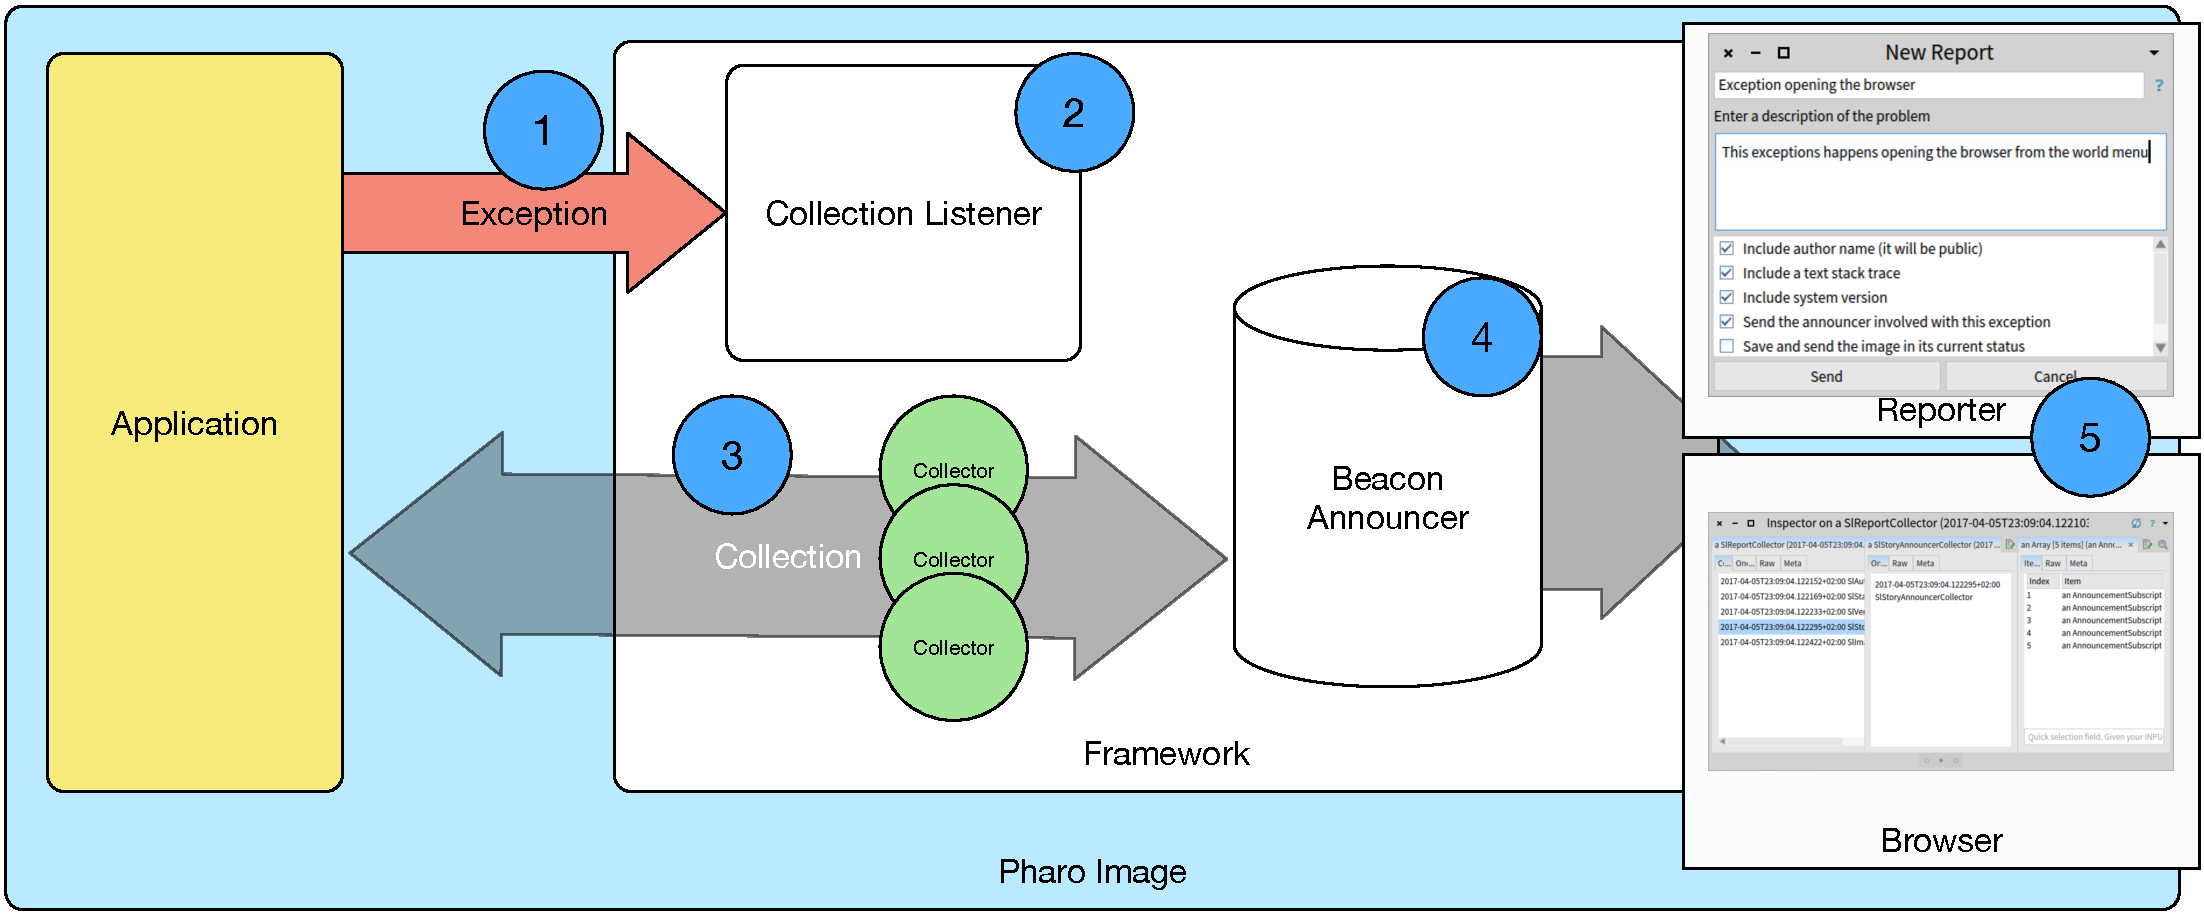
\includegraphics[width=.9\linewidth]{reified/process}
  \caption{The workflow to collect data using collectors, showing the architecture of \sln}
  \label{fig:architecture}
\end{figure*}

We now present the implementation details of the framework for the Smalltalk programming language, while \secref{sec:reified-summary} we will also discuss the challenges of generalizing such an approach to other programming languages.

In implementing our framework, we need to consider a number of aspects pertaining to the control of the system, first of all the ability to directly catch errors and manipulate its context to extract the relevant data in a usable state.
Accomplishing such a task is strongly dependent on the programming language of choice with the result that the amount of technical details that can be considered is humongous, and out of the scope of this work.
We implemented and test the effective feasibility of our approach using \pha.
The fact that the whole system is described using objects allows us to easily inspect faulty states of the system by interacting through the \texttt{Context} object, and simplifies the reification process of the interesting entities.

While the use of \pha enables full flexibility and control over the execution of a program, one may wonder whether this hinders the applicability of the approach to more general examples.
We believe that this does not affect the possibility to implement an analogous framework for a different programming language.
\secref{sec:reified-summary} contains a deeper discussion about the generalizability of our approach.

\subsection{Implementation Details}

The abstractions in the \pha environment concern the whole runtime of the system, allowing to inspect and manipulate it by querying objects.
The main benefit of \pha is that we can freeze the execution of a program, and easily access the whole system status at the moment of the interruption.

The principal element we are interested in is the \entity{thisContext} variable.
This special variable stores an instance of \entity{Context}, an object that mimics the behavior of an \textit{activation record} that contains all the information about the current execution of the program, such as the list of the variables in the scope, the method that is currently executing, the class that owns the method, the program counter of the line of code we are executing, and other information useful in describing the running session.


\subsubsection{Implementing Collectors}

We designed our framework around the idea of \emph{collectors}.
In \secref{sec:reified-design} we defined a collector as an entity that knows how and when to collect data, and that provides a description for this data.
By following the object-oriented nature of \pha we can implement a collector as a class.
While having a class for each collector might seem overkill, that might eventually bloat the system rather than supporting maintenance, it has the advantage of providing full control to the user of our framework, granting the flexibility to select the data she wants to observe.
The whole strategy can be encapsulated in a single class, thus decoupling the collector from the source code it is observing and providing a behavior that can be plugged and un-plugged seamlessly.

We define the class \entity{DataCollector}, that defines the template for implementing a collector.
A user can create a new collector by subclassing this class, and implementing four methods that define its behavior:

\begin{description}

\item \method{\#tag} --- the name of the method, used to reference the collected data by means of an automated approach;

\item \method{\#description} --- a short description of the data collected by the class, displayed to the user when presenting the data or when asking for permission to send the data to the issue tracking system;

\item \method{\#when:} --- an expression that evaluates the state of the system to decide whether or not the collector is interested in observing the current context;

\item \method{\#initializeFrom:} --- the main method that implements the strategy for extracting the data.

\end{description}

Both the \method{\#when:} and \method{\#initializeFrom:} method receive an object of type \entity{Context} as parameter, that contains the references to the current execution environment with all the variable in scope and the invocation stack.
While the \method{\#when:} method determines if the context is interesting and needs to be collected, it is its responsibility of \method{\#initializeFrom:} to construct what needs to be collected, \eg an object representing an abstraction of the system state.

%By defining four methods, a developer is able to instrument its code to detect and observe the exceptions triggered by her code.

In \secref{sec:reified-stories} we show three use cases for a collector, with an example implementation that presents the source code for implementing a strategy.


\subsubsection{Triggering the Collection}

The collection approach needs an entry point that signals the system that we might want to record the current context and extract the status of an application.
We decided to trigger the collection in two cases: For the handling of errors, or arbitrarily triggered by the user.
The former is invoked automatically whenever an unhandled exception occurs, while the latter needs to be explicitly invoked using the \sln public APIs.

\figref{fig:architecture} shows a diagram of the flow of the data from the collection to its usage.

The collectors evaluate whether they should activate, and potentially perform the data collection.
Once the collection is complete, the framework composes a \entity{Report} object and announces its creation using \bea,\seeurl{www.smalltalkhub.com/\#!/$\sim$Pharo/Beacon} an announcement-based (\ie publish/subscribe) logging framework for \pha.
\bea broadcasts messages to the system to inform the interested tools of the presence of a report.

By collecting complex entities in form of objects, rather that text, our approach allows to initiate a conversation with the system and a systematic and progressive exploration of the errors, rather than just providing a partial report of the exception.
This allows us to observe the properties of the objects and deal with them in a customized way.

\subsection{Using the Data}\label{sec:reified-tools}

Once a report is broadcast, every interested tool will receive the data.
This behavior is intended to further improve the customizability of the framework, allowing the developer of a system to refine their tools for quickly inspect the data collected about their code, as proposed by guideline (3).

The two applications proposed by default by our approach consist in a local data browser, and a customized reporter.
If a user is interested in browsing the data locally, for example during the development phase of a project, she can inspect the contents of the report objects.
Moreover, she can exploit the tools provided by the \pha ecosystem, like the \emph{Glamour Toolkit}~\cite{Girb2013a} to create custom visualizations of the data to support the browsing session.

On the other hand, if the user of the system is not the developer of the original code, the system can serialize the report and send it to the issue tracker with a comment of the user explaining how she encountered the error.
\figref{fig:reporter} shows the interface for submitting a report: to protect the privacy of the users, as described by guideline (5), a user can read the description of the collected data and decide whether she wants to send it or to exclude it from the report.

\begin{figure}[ht]
  \centering
  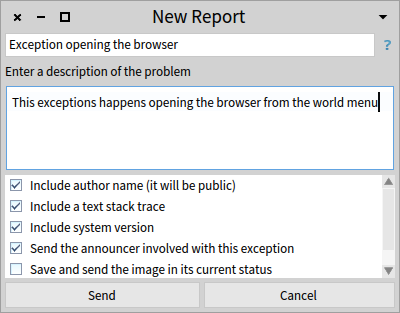
\includegraphics[width=.55\linewidth]{reified/reporter}
  \caption{The reporting window for \sln, where the user can select the data that she wishes to report and add a description}
  \label{fig:reporter}
\end{figure}

In the next section we show how to implement a collector to solve common development problems.


\section{The Framework at Work}\label{sec:reified-stories}

In this section we show how to employ our framework to support debugging and program maintenance.
We present three scenarios and show how to collect domain-specific information from different environments.
We show how accessing specific information can support developers in quickly understanding the cause of a defect and the behavior of a piece of code.

In \secref{sec:reified-story-announcer} we present an in-depth case study together with a possible implementation showing how our approach can support debugging errors in applications using the Announcer framework, a messaging framework that reduces coupling but that might introduce non deterministic behavior; In \secref{sec:reified-story-testing} we outline how to collect data when running a test suite, and how its usage can integrate the current practices in continuous integration of deployed application and support automation; \secref{sec:reified-story-libraries} presents a brief discussion on how using \sln can benefit debugging third party libraries in the context of complex entities.

\subsection{The Announcer Story}\label{sec:reified-story-announcer}

The continuous evolution of the requirements of a software system results in a codebase that grows constantly, both in size and complexity.
To tame this problem, developers design software systems using a modular architecture, where large tasks are split into smaller functionalities, so that complex operations can be managed by composition of small entities, with a defined operational context and limited to few specific responsibilities.
In such a scenario, dispatching messages is fundamental to exchange information among the components and orchestrate the behavior of the modular system.
While the gained modularity is invaluable in developing, testing, and maintaining a system, it comes at a cost: Integrating different modules can show errors generated by the interaction between components and, depending on how the communication is performed, might present non-deterministic behavior.
Since the flow of the execution is distributed into different locations, tracking the source of a defect can become a complicated and time consuming task.
To enable communication among system components, \pha offers the \emph{Announcer} framework: a tool that implements an improved version of the Observer pattern and reduces coupling.
When an entity in the system wants to communicate a message to other entities, it instantiates an \emph{announcer}.
The entities interested in receiving a notifications can then register to the relevant announcer, specifying the type of events they want to observe.
To broadcast a message, a component can create a new \emph{announcement} and send it to the announcer, that dispatches it to the subscribed entities.

The strength of the Announcer framework is that announcements are treated as first class entities: once it occurs, an event is represented by an object that can contain arbitrary data and the subscribers that registered for that event can interact with it using its public interface.
The use of announcements to manage the communications between different applications has numerous advantages, like loosing the coupling between the publisher of an event and its subscribers, and is a recommended best practice in developing an application in \pha.

However, as discussed earlier, fragmenting the control flow of the program into a set of disjoint components carries the drawbacks of event-based programming with the consequence that finding the right fragment of code that is responsible for an error becomes a convoluted process of navigating through the callbacks to find the correct location in the system.
This complicates the debugging process, as understanding how an announcement propagates through the system and affects its status, requires accessing information that is not usually accessible by simply inspecting the stack trace generated by an exception.
The problem with debugging an announcement is that it follows a different logic than the usual sequential style of the rest of the system.
Therefore, while all the information necessary to understand an error is available during an exception, this is usually not exposed by the tools used to catch and report the errors, like the system logger, hence not exploitable to understand and fix the problem.
In particular, to understand an error generated during the broadcasting of an announcement it is not enough to observe the current stack of method calls: As such a structure would only contain information about the subscriber that generated the error, thus hiding the information about the behavior of the other subscribers.
While this might still be sufficient to support debugging of simple problems, it lacks all the collateral information to create the big picture of the status of the announcer and its subscribers.


\subsubsection{Usage of Announcements}

\figref{fig:announcer-report} shows a bug report submitted to the \pha issue tracker, describing a problem with a tool where selection an item from a menu would trigger the opening of two duplicate windows, instead of one.

\begin{figure}[t]
  \centering
  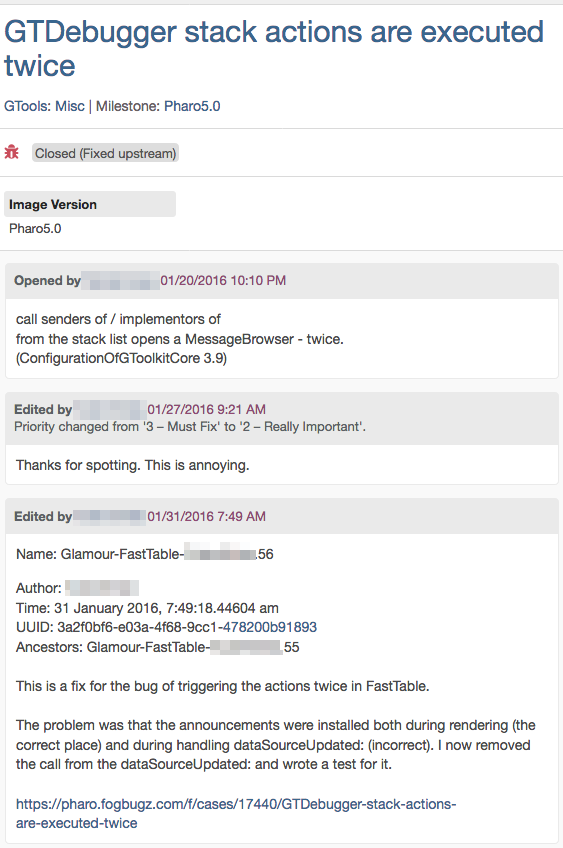
\includegraphics[width=.6\linewidth]{reified/announcer-report-small}
  \caption{A bug report describing a duplicated behavior caused by an entity being registered twice to an announcer}
  \label{fig:announcer-report}
\end{figure}

During the discussion it becomes soon clear that the incident is compatible with the case of an entity registered twice in the announcer responsible for opening the window.
The debugging process consists in hunting down the entity that contains the double registration and remove one of the two snippets of code that perform the subscription.
While this case is not directly a consequence of an exception, it shows how debugging the behavior of code using announcements can be tricky, and that further support from the development tools would probably be preferred.
We therefore conducted a brief experiment to investigate how common are problems involving announcements in the exceptions that developers usually trigger while writing code.

For this purpose, we inspected the data collected through \sln, the tool we presented in \chref{ch:stacktraces} to intercept stack traces from development exceptions and report them to a central server to support debugging~\cite{DalS2015a}.
We considered the stack traces collected from 10 June 2014 to 28 February 2017.
\tabref{tab:stack-traces} shows a summary of the collected data.

\begin{table}[ht]
\centering
\caption{Summary of the collected stack trace data}
\rowcolors{1}{tablefirstrow}{tablesecondrow}
\begin{tabular}{lr}
\hline
Oldest stack trace & 10 June 2014 \\
Newest stack trace & 28 February 2017 \\
\# of days & 994\\
\# of developers & 257\\
average \# of traces per day & $\sim$41\\
\# of stack traces & 41,129 \\
\# of traces involving announcements & 4,840 \\
\% of traces involving announcements & $\sim$12\% \\
\hline
\end{tabular}
\label{tab:stack-traces}
\end{table}

% \begin{table}[ht]
% \centering
% \caption{Summary of the collected stack trace data}
% \rowcolors{2}{tablefirstrow}{tablesecondrow}
% \begin{tabular}{l|r}
% \hline
% Oldest stack trace & 10 June 2014 \\
% Newest stack trace & 28 February 2017 \\
% \# of days & 994\\
% \# of developers & 257\\
% average \# of traces per day & $\sim$41\\
% \# of stack traces & 41,129 \\
% \# of traces involving announcements & 4,840 \\
% \% of traces involving announcements & $\sim$12\% \\
% \hline
% \end{tabular}
% \label{tab:stack-traces}
% \end{table}


% \begin{table}[ht]
% \centering
% \caption{Summary of the collected stack trace data}
% \rowcolors{2}{tablefirstrow}{tablesecondrow}
% \def\arraystretch{1.1}
% \begin{tabularx}{\linewidth}{X|r}
% \hline
% Oldest stack trace & 10 June 2014 \\
% Newest stack trace & 28 February 2017 \\
% \# of days & 994\\
% \# of developers & 257\\
% average \# of traces per day & $\sim$41\\
% \# of stack traces & 41,129 \\
% \# of traces involving announcements & 4,840 \\
% \% of traces involving announcements & $\sim$12\% \\
% \hline
% \end{tabularx}
% \label{tab:stack-traces}
% \end{table}

% %\def\arraystretch{1.1}
% \begin{tabularx}{\linewidth}{X|r}
%
% \rowcolor{gray!30} \textbf{Metric} & \textbf{Value} \\ \hline
% Number of Interaction Events & 238,741 \\
% Number of Developers & 18 \\
% Number of Interested Classes (in the \pha distro) & 2,988 (965) \\
% Number of Different Event Types (total) & 13 (32)
% \end{tabularx}
% \end{table}


The collecting tool can be set to submit every exception automatically, or to ask the developer whether she wants to explicitly submit it.
The stack traces collected come from exceptions generated by users of the \pha platform from their daily development activities.
We collected 41,129 stack traces from 257 different developers, on a time period of almost three years.
We queried the collected data looking for references to \textit{AnnouncementSubscription}, the class responsible to dispatch the announcement to the registered entities, and we found that 4,840 stack trace contain at least one reference to this class.

Such a result means that almost 12\% of the exceptions that were collected by our tool as a result of a system exception, involved the usage of the Announcement framework.
While this result does not imply that the framework is directly responsible or involved with the error, it shows that more than one exception every ten has in its source a relation with an announcement.
This hints that the scenario is frequent enough to require a dedicated support by the debugging tools, not only to correct errors, but also to help understanding the status of the system during its execution.


\subsubsection{Implementation of the collector}

Our goal is to use a model able to collect and present domain-specific information about the message dispatching.
We can use this information to refine the inspection tools used to investigate the system, or to create bug reports capable of representing the exception with further details that are not representable using the stack trace generated by the exception.

We can accomplish the task using a custom extension of \sln to collect runtime data that describes the environment of an announcement.
To implement the collector we need to define the strategies to activate for its activation and to describe the data extraction.
There are two main scenarios that can lead to errors using an announcer: \figref{fig:announcer-report} showed how an entity being registered twice to an announcer can lead to weird bugs, while the potentially non-deterministic nature of an announcer, given by the fact that messages are dispatched in no specific order, can cause bugs that are hard to reproduce.
We therefore decide to observe four features:
%
\begin{inparaenum}[(1)]
  \item the subscribers of the announcer listening for the specific announcement,
  \item the announcement being dispatched,
  \item the subscriber that generated the exception, and
  \item the list of subscribers that already received the announcement compared to the list of subscribers that did not receive it yet.
\end{inparaenum}
%
\figref{fig:announcer-code} shows the implementation of \textit{AnnouncerCollector} the class responsible for gathering data about an announcement.

\begin{figure}[t]
\centering
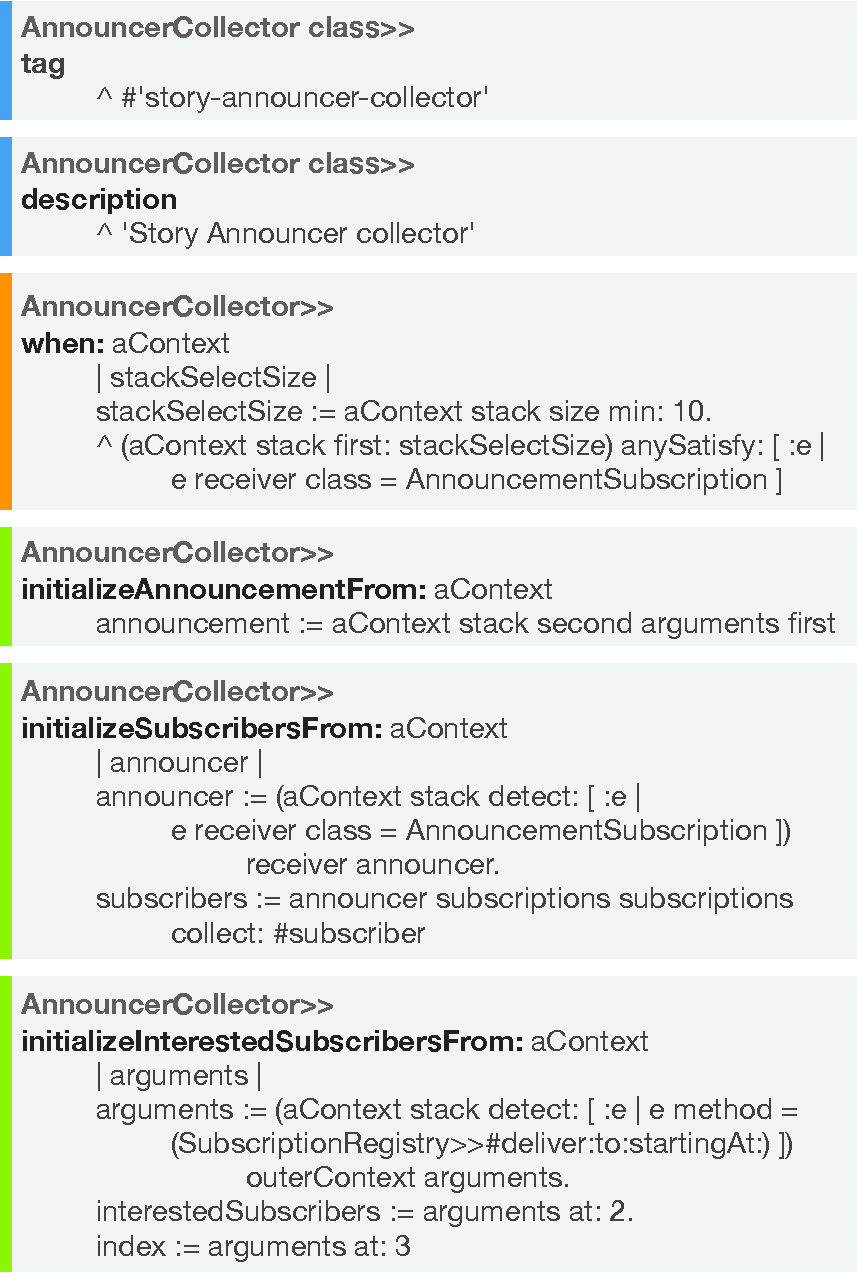
\includegraphics[width=.6\linewidth]{reified/announcer-collector}
\caption{The Smalltalk code implementing the extraction strategies for the Announcer collector}
\label{fig:announcer-code}
\end{figure}

The methods \method{\#tag} and \method{\#description}, from the class side of AnnouncerCollector describe the collector, for indexing and user interaction purposes.
The method \method{\#when:} checks the current context object and verifies if there is a reference to a \entity{AnnouncementSubscription} object in the first 10 lines of the method invocation stack, to ensure that announcements are involved in the exceptions in the immediate surroundings of the current context.
The other three methods are invoked during the initialization of the collector, once the \method{\#when:} returned a positive response:
\method{\#initializeAnnouncementFrom:} extracts the information of the announcement that triggered the broadcasting process, together with possible data that it was supposed to deliver;
\method{\#initializeSubscribersFrom:} extracts all the entities registered to the announcer, regardless of the kind of announcement they are listening to;
\method{\#initializeInterestedSubscribersFrom:} extracts the distribution list of the announcer.
Since this data is collected during the execution time, this list contains the order in which this announcement is being distributed.
Moreover, the method also extracts the index of the current entity: In this way the developer can access the list of the entities that already received the announcement and the one of the entities that did not receive the message, thus easing the detection of possible conflicts between different subscribers.

The data collected by the Announcer collector provides a detailed picture of the status of a program, in an environment where it is usually hard to understand what causes the code to fail, thus giving the developer an immediate overlook on the dispatching of the messages.
Moreover, the data collected are still first-class entities of the system, that can be further queried to extract data: this process allows to retain the maximum amount of information for the longest time needed, so that it can be inspected during an exception or flattened into a textual format for the submission to an issue tracking system.
If the system allows it, the entities can also be serialized and sent to the issue tracker, so that the maintainers of a software can navigate the errors generated by the users with a much higher degree of flexibility and introspection on the data than just plain text log files.

Stepping aside from the specific case of the announcer, this example shows how our framework can help developers to easily extend the behavior of the logging mechanism to collect domain-specific data that pertains to the software they develop.
By distributing a software together with some custom collectors, a developer can effortlessly select the exceptions that are caused by her software, collect relevant data ---with the consent of the user--- and browse it to debug the error.

\subsection{The Testing Story}\label{sec:reified-story-testing}
%Collectors can be put in place to refine and augment test execution, impacting the way we conduct tests both in an interactive fashion or automatically with a continuous integration server.

Bug fixing is an essential part of software development: Therefore, part of the development effort consists in ensuring that a piece of code behaves in the intended way as the codebase changes.
The main tool for this purpose is represented by unit and integration tests, that help the developers to immediately spot unexpected behaviors and locate the responsible components.
The use of test cases plays a central role in developing software, especially since the advent of agile techniques like \emph{Test Driven Development} (TDD) and continuous integration~\cite{Beck2001manifesto}.
The former expects the developer to write a test mapping the expected outcome before writing the code to perform the task, while the latter consists in automating the testing process by integrating it in the development workflow.

We analyze the possible role of our approach based on collectors within the combination of these two specific contexts.
While in the case of TDD the developer has immediate access to the error and its context, running a test suite to check the whole codebase can generate errors that are complex to frame in the correct context.
Moreover, in the case of continuous integration, where the tests do not run on the machine of the developer but are executed on a remote server, developers only have access to the output of the tests, which usually consist on textual reports.
This happens for example if a project adopts a continuous integration service like Travis CI,\seeurl{https://travis-ci.org/} that performs a full run of the tests every time the project is updated, and then sends a report of the outcome to the developers.

When a test fails, however, the trace of the error is flooded into the log messages generated during the build process, requiring time to identify and filter the relevant information.
Once a developer finds information about the failed test, she has to read the text output to understand what was the possible cause of the failure, return to her development environment, reproduce the failed case, locate the source of the defect and fix it.
This process might still be lightweight in the case of simple defects in small projects with one developer, but as the organization of the project grows in complexity, reproducing and locating the issue can become a burden that costs a significant amount of time.
We can improve this scenario by introducing \sln collectors.
By writing a small amount of code, developers are able to extract the specific information they are interested in about a failing test.
Writing a collector for a test case is simple: Smalltalk uses the testing suite called \textit{SUnit}~\cite{Beck1994a}, where each test class is a subclass of \textit{TestCase}.
We can therefore define the \textit{\#when:} method to activate the collector if there is an instance of such class in the invocation stack of the exception.
We can then write the extraction strategies to gather the status of the part of the system that is subject of the testing, or simply extract the whole context storing all the objects in the stack.

Using collectors, our framework allows developers to generate automatic reports that can be sent and managed in an automated fashion, guaranteeing the reliability and quality of the data.
This data can then be serialized using a framework like \textit{STON},\seeurl{https://github.com/svenvc/ston} so that a developer can still access part of the objects involved with the exception.
The use of objects allows to directly communicate with the status, without having to revert to text mining techniques to infer the involved entities from textual logs.

For example, when a test fails, \entity{SUnit} generates an \entity{AssertionFailure} exception.
Catching this exception allows to access the context of the test, containing the erroneous result and the local variables, especially the class that is object of the test.
By serializing and sending this information, we can collect and group this data from all the failed test to generate an automatic report containing all the objects in a wrong state, and navigate it to identify the cause for the failing tests.

%There is a drawback in customizing collectors to detect specific information in test suites: It is not always possible to define a strategy that is specific enough to collect relevant information, but at the same time broad enough to not require writing a collector for each test case, which would clearly be unfeasible.
Sometimes, however, observing just the tested object is not enough: The cause of the failure might be hidden in the underlying system, or the object would reference volatile resources, like database connections or remote sockets.
In this case we can adopt a different approach and offer a default option to cover the most difficult cases.
Leveraging the Smalltalk approach of the \emph{image}, that can be frozen and saved in a particular state and later reopened with the exact same state, we can write a collector that, when an exception occurs, saves the image and sends it to a central server with a report containing metadata about the exception.
Using this approach, when a build fails to pass the tests, the developer can browse the repository of images, download the relevant one and open it on its local machine.
The concept is similar to using \emph{Docker}\footnote{\url{https://www.docker.com/}} to deploy applications, where the system runs in an isolated controlled environment, independent from the host operating system.

Either using the automatic report generated by the failing tests, or downloading directly the image containing the error, developers can observe details of the system at the moment of the failure, thus shortening the time required to identify the steps to reproduce the error, and reduce the maintenance cost.

\subsection{Debugging Third Party Libraries}\label{sec:reified-story-libraries}

The last example on the usage of the framework shows how a developer of a third party library can benefit from implementing a collector observing for specific data about her project.
In the Smalltalk ecosystem, \emph{Roassal}\footnote{\url{http://agilevisualization.com/}} is a large and vastly used visualization engine made to ``visualize and interact with arbitrary data, defined in terms of objects and their relationships''~\cite{Aray2013a}.
Roassal codebase consists of more than 800 classes and almost 6,000 methods, and is constantly evolving and improving using the feedback of the community.
Maintaining such a large project is a complicated task, as tracing and addressing the errors experienced by the users can become like hitting a moving target, especially since Roassal integrates with other tools and because the community is usually split among stable, legacy, and development releases.

Understanding what triggered an error and rebuilding the environment to reproduce it can become quite painful, as the developers need information that might not be easy to provide.
Using a coarse-grained approach as the one we described in \secref{sec:reified-story-testing} would not fit this scenario, as asking the user to submit the whole image would generate a lot of traffic that would be hard to manage, without considering that the image could contain sensitive data, like private source code, that a user might not want to share.

The maintainers of Roassal can improve this situation by observing data specifically related the the model of the engine.
By detecting either when an exception occurs involving an object that is a subclass of \textit{RTObject}, or by checking if it happens in the context of a builder ---a Roassal object responsible for generating a visualization from a collection of data---, a collector can determine if there is some information about Roassal available, that can be collected and reported.

By collecting domain-specific information, the maintainers can get a much more detailed picture of the error, and restrict the possible causes to the ones compatible with the collected data without the need to access the actual data of the user.
For example, by knowing the number of nodes that a visualization is rendering, one could tell if the error is due to a memory problem, or if the visualization has scalability issues.
Instead, knowing the settings that were used to configure a builder can tell if there is a bug in the builder's code, or if the public API is poorly designed and therefore often misused by the users.
Finally, knowing the kind of data that a visualization received can help in finding if there is a bug in managing objects of different (specific) types.

By shipping their own collectors for observing their code, developers can support debugging in the context of the project, therefore reducing the time required to understand an error and lowering the cost for maintenance.


\section{Summary}\label{sec:reified-summary}

We presented an approach to define ad-hoc collection of runtime data to support debugging.
By extending our framework, a developer can define a custom strategy to gather domain-specific knowledge that follows the model of the application she wants to observe.
By preserving the structured, object-oriented nature of the collected data, rather than serializing the information to text, we are able to query the state of a program  and observe it by filtering the data we are interested in, resulting in both more expressive and less bloated reports.
Such capabilities of observing a system enable to create flexible inspection tools, that are able to get a deeper representation of the execution context of a piece of software.

By giving the possibility to report and collect specific information from the system, \sln offers data that is more reliable that a stack trace submitted by a user, and allows to deal with the collected data in an automated fashion, giving the possibility to programmatically perform tasks that would otherwise consume time of the developers and weight on the cost of maintenance.
Moreover, providing a defined structure for execution data, our framework allows to perform a number of analyses without having to resort to information retrieval and text mining techniques to clean the data, but allows to talk directly with the collected entities that map the original data.

Finally, dealing with data that is not flattened allows to perform a progressive inspection of a report, enabling the discoverability of complex data and structuring the debugging session as a browsing process to select the data needed by the developer fixing a bug.


\subsubsection{Generalizability of the approach}

As we explained in \chref{ch:pharo}, we developed our approach using \pha.
The strong reflection and inspection capabilities of the platform allowed us to inspect the whole status of the system, retrieving valuable information about the whole execution context of the software.

Given these premises, one might wonder (1) why should this approach be relevant in the \pha ecosystem, and (2) if it is still relevant outside \pha, when trying to apply it to other programming languages.

To answer question (1), this framework comes after a long collaboration with the \pha community, to understand the types of errors that users get during the use and the development of the platform.
As we discussed through the chapter, the data collection mechanism can be integrated with the issue tracking system of a project, allowing the developers of a project to integrate \sln in their workflow, supporting debugging and maintenance tasks.
About question (2), we believe that it is possible to implement such an approach also in other programming languages.
The \pha system makes the perfect candidate to test such a framework, easing the implementation process by providing the APIs to talk with the system and the tools to navigate the collected data, but the use cases we have shown in \secref{sec:reified-stories} can be implemented with any language with reflective capabilities.

There is also an interesting aspect to consider pertaining to how we used a collector in section \secref{sec:reified-story-testing} to save and submit the whole \pha image.
Given the current interest in DevOps technologies like Docker\footnote{\url{https://www.docker.com/}}, it is possible to execute an application in a Docker container, stop it and save its status during an exception, and submit the image of the application to a remote server.
Analyzing the stored data would not be simple, as there is a lack of tools to access the state of applications in these circumstances, but our approach could be an interesting match for these similar scenarios.


\subsection{Next Steps}

Building collectors to observe specific parts of the system can improve the workflow of debuggers, and reduce maintenance costs.
The regular collection of domain-specific data can provide statistics on the frequency of errors in selected parts of the system, and hint how the users use a software, hence helping developers not only to debug a system, but also to optimize the existing code and improve the API.
%We plan to propose \sln for the integration with the next standard \pha distribution, proposing some generic collectors to support standard difficult debugging tasks, like the one that we proposed in \secref{sec:reified-story-announcer} about the Announcer framework.
%By reaching a larger user base we can collect more specific data about the usage of the tool, refine further the collectors implementation and evaluate the impact of such an approach in daily development activities.

We envision a future where development activities are supported by the system using the language of the system, not resolving to flat and bloated chunks of plain text that represent the side effects of the code, but rather first-class entities that narrate the exact status of a program.
Starting a conversation with the entities we can develop a paradigm of programming that focuses on the models and their interactions, rather than manipulating strings, and achieve a programming environment that is really live and responsive.


\subsubsection{The Road So Far...}

In this chapter we put in place a platform to collect detailed domain-specific information about components of a system.
In the next chapter we present an approach to employ the information collected about a system in a tool for browsing the history and the evolution of a software system.

%  %!TEX root = ../tommaso-thesis.tex
%!TEX spellcheck = en_US


% status color definition
\definecolor{active}{HTML}{FF6600}
\definecolor{work needed}{HTML}{FF0000}
\definecolor{closed}{HTML}{888888}
\definecolor{resolved}{HTML}{666666}
\definecolor{working on}{HTML}{3388FF}
\definecolor{on hold}{HTML}{55FFFF}
\definecolor{unknown}{HTML}{D3D3D3}


\chapter{Visual Analytics of Bug Repositories}\label{ch:visualize}
% \coolchapter{in*Bug}{Visual Analytics of Bug Repositories}{ch:visualize}


Bug tracking systems are used to track and store the defects reported during the life of software projects.
The underlying repositories represent a valuable source of information used for example for defect prediction and program comprehension~\cite{stor1999a}.
However, as we mentioned in \chref{ch:introduction}, bug tracking systems store and present the actual bugs essentially in textual form, which is not only cumbersome to navigate, but also hinders the understanding of the intricate pieces of information that revolve around software bugs.
We begin our journey towards an improved representation for a bug report by analyzing existing bug repositories, to investigate where the information that they contain can be actually leveraged to improve the knowledge that we have on the system.

In this chapter we present \ib, a web-based visual analytics platform to navigate and inspect bug repositories.
\ib provides several interactive views to understand detailed information about the bugs and the people that report them.
% The tool can be downloaded at \textit{http://inbug.inf.usi.ch}


\structure

\secref{sec:visualize-intro} introduces the issues of dealing with data in issue trackers.
\secref{sec:visualize-details} presents in detail the views that compose \ib.
\secref{sec:visualize-summary} concludes the chapter summarizing what we learned visualizing issue tracking systems.


\newpage

%%%%%%%%%%%%%%%%%%%%%%
\section{Accessing Bug Repositories}\label{sec:visualize-intro}
%%%%%%%%%%%%%%%%%%%%%%

Due to the complexity and size of non-trivial software projects, the development of a system is always accompanied by software defects, or bugs.
To manage these defects, modern software projects use bug tracking systems (also known as bug trackers or issue trackers), such as Jira or Bugzilla.
With bug trackers, end users and developers can report bugs they encountered while using the system, usually by means of custom web interfaces, where one can enter details about a specific bug, creating a so-called \emph{bug report}.
A typical bug report, such as the one depicted in \figref{fig:fogbugz-example}, contains information about \begin{inparaenum}[(1)] \item the title and id of the bug, \item the user who reported the bug and the people involved in its history, \item its current status, \item its opening and closing date, \item its last modification date, \item the project to which the bug report pertains, \item events (such as changes of the people assigned to the bug report, etc.) during the life cycle of the bug, etc. \end{inparaenum}
The example bug report depicted in \figref{fig:fogbugz-example} is from a specific bug tracker, FogBugz \footnote{\url{http://www.fogcreek.com/fogbugz/}}, but it does not differ significantly from the reports recorded with other bug trackers.

\begin{figure}[ht]
\centering
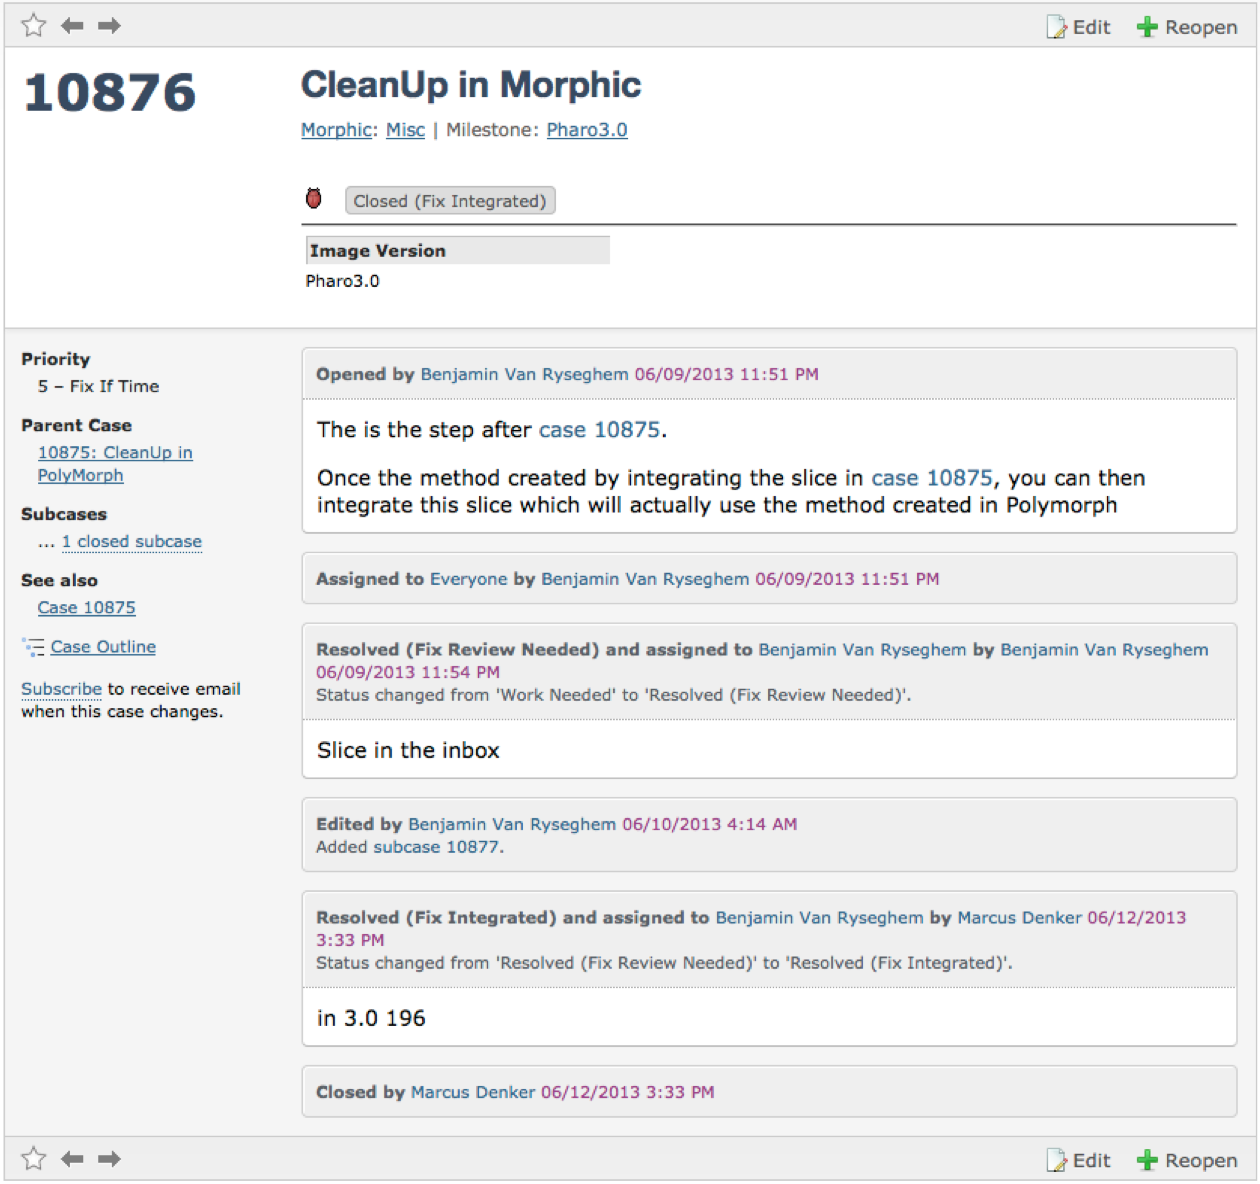
\includegraphics[width=.95\linewidth,trim=0 300 0 0,clip=true]{Images/visualize/fogbugz-screen}
\caption{Example bug report in the FogBugz bug tracking system.}
\label{fig:fogbugz-example}
\end{figure}

Various researchers have mined and used the information stored by bug trackers to perform several types of analyses, such as identifying duplicate bug reports~\cite{Wang2008a}, measuring the quality of a report~\cite{Zimm2010a}, predicting future defects~\cite{DAmb2012a}, performing traceability linking~\cite{Biss2013a}, locating features~\cite{Dit2013a}, ameliorating bug triaging decisions~\cite{Anvi2006a}, etc.
The actual goal however is to ease the life of developers in the handling of bug reports, as part of the development process.

One problem is that bug reports are disconnected from the software system they pertain to, and it is up to the developers to restore the link between a bug report and the interested components of a system.
Another problem is that bug reports, such as the one depicted in \figref{fig:fogbugz-example}, are displayed on individual web pages that list their properties, making them cumbersome to handle and making it also difficult to obtain a ``big picture'' of the existing open bug reports and how they affect the system they pertain to.
Moreover, this information is stored and presented as text, which makes it hard to understand the properties of a bug report.

We present \ib, a web-based bug analytics platform, that eases the inspection, navigation, and comprehension of bug repositories, mostly by means of interactive visualizations.
\ib provides an entry-level big picture overview to browse the content of a repository, and a detailed, complementary, interactive, and finer-grained view to understand detailed information about the bugs and the people that report them.

Other researchers have produced custom visualization of bugs, such as D'Ambros \etal~\cite{DAmb2007a,DAmb2007b} who proposed visualizations that tried to depict the complex information revolving around bugs, which are de facto independent entities when it comes to program comprehension, and not mere side effects of the evolutionary process that software systems are subjected to.
While D'Ambros et al. only created standalone depictions of information taken from BugZilla, our goal with \ib is to depict live data from a bug tracker, namely FogBugz.
The goal of \ib is to offer a complementary view to inspect and analyze information pertaining to bugs reported in the context of the many projects that make up a software ecosystem.
We built \ib around the issue tracking system of the \pha open-source community.

We now present the features of \ib, discuss its current implementation, and illustrate its usage.


\begin{figure*}[t]
\centering
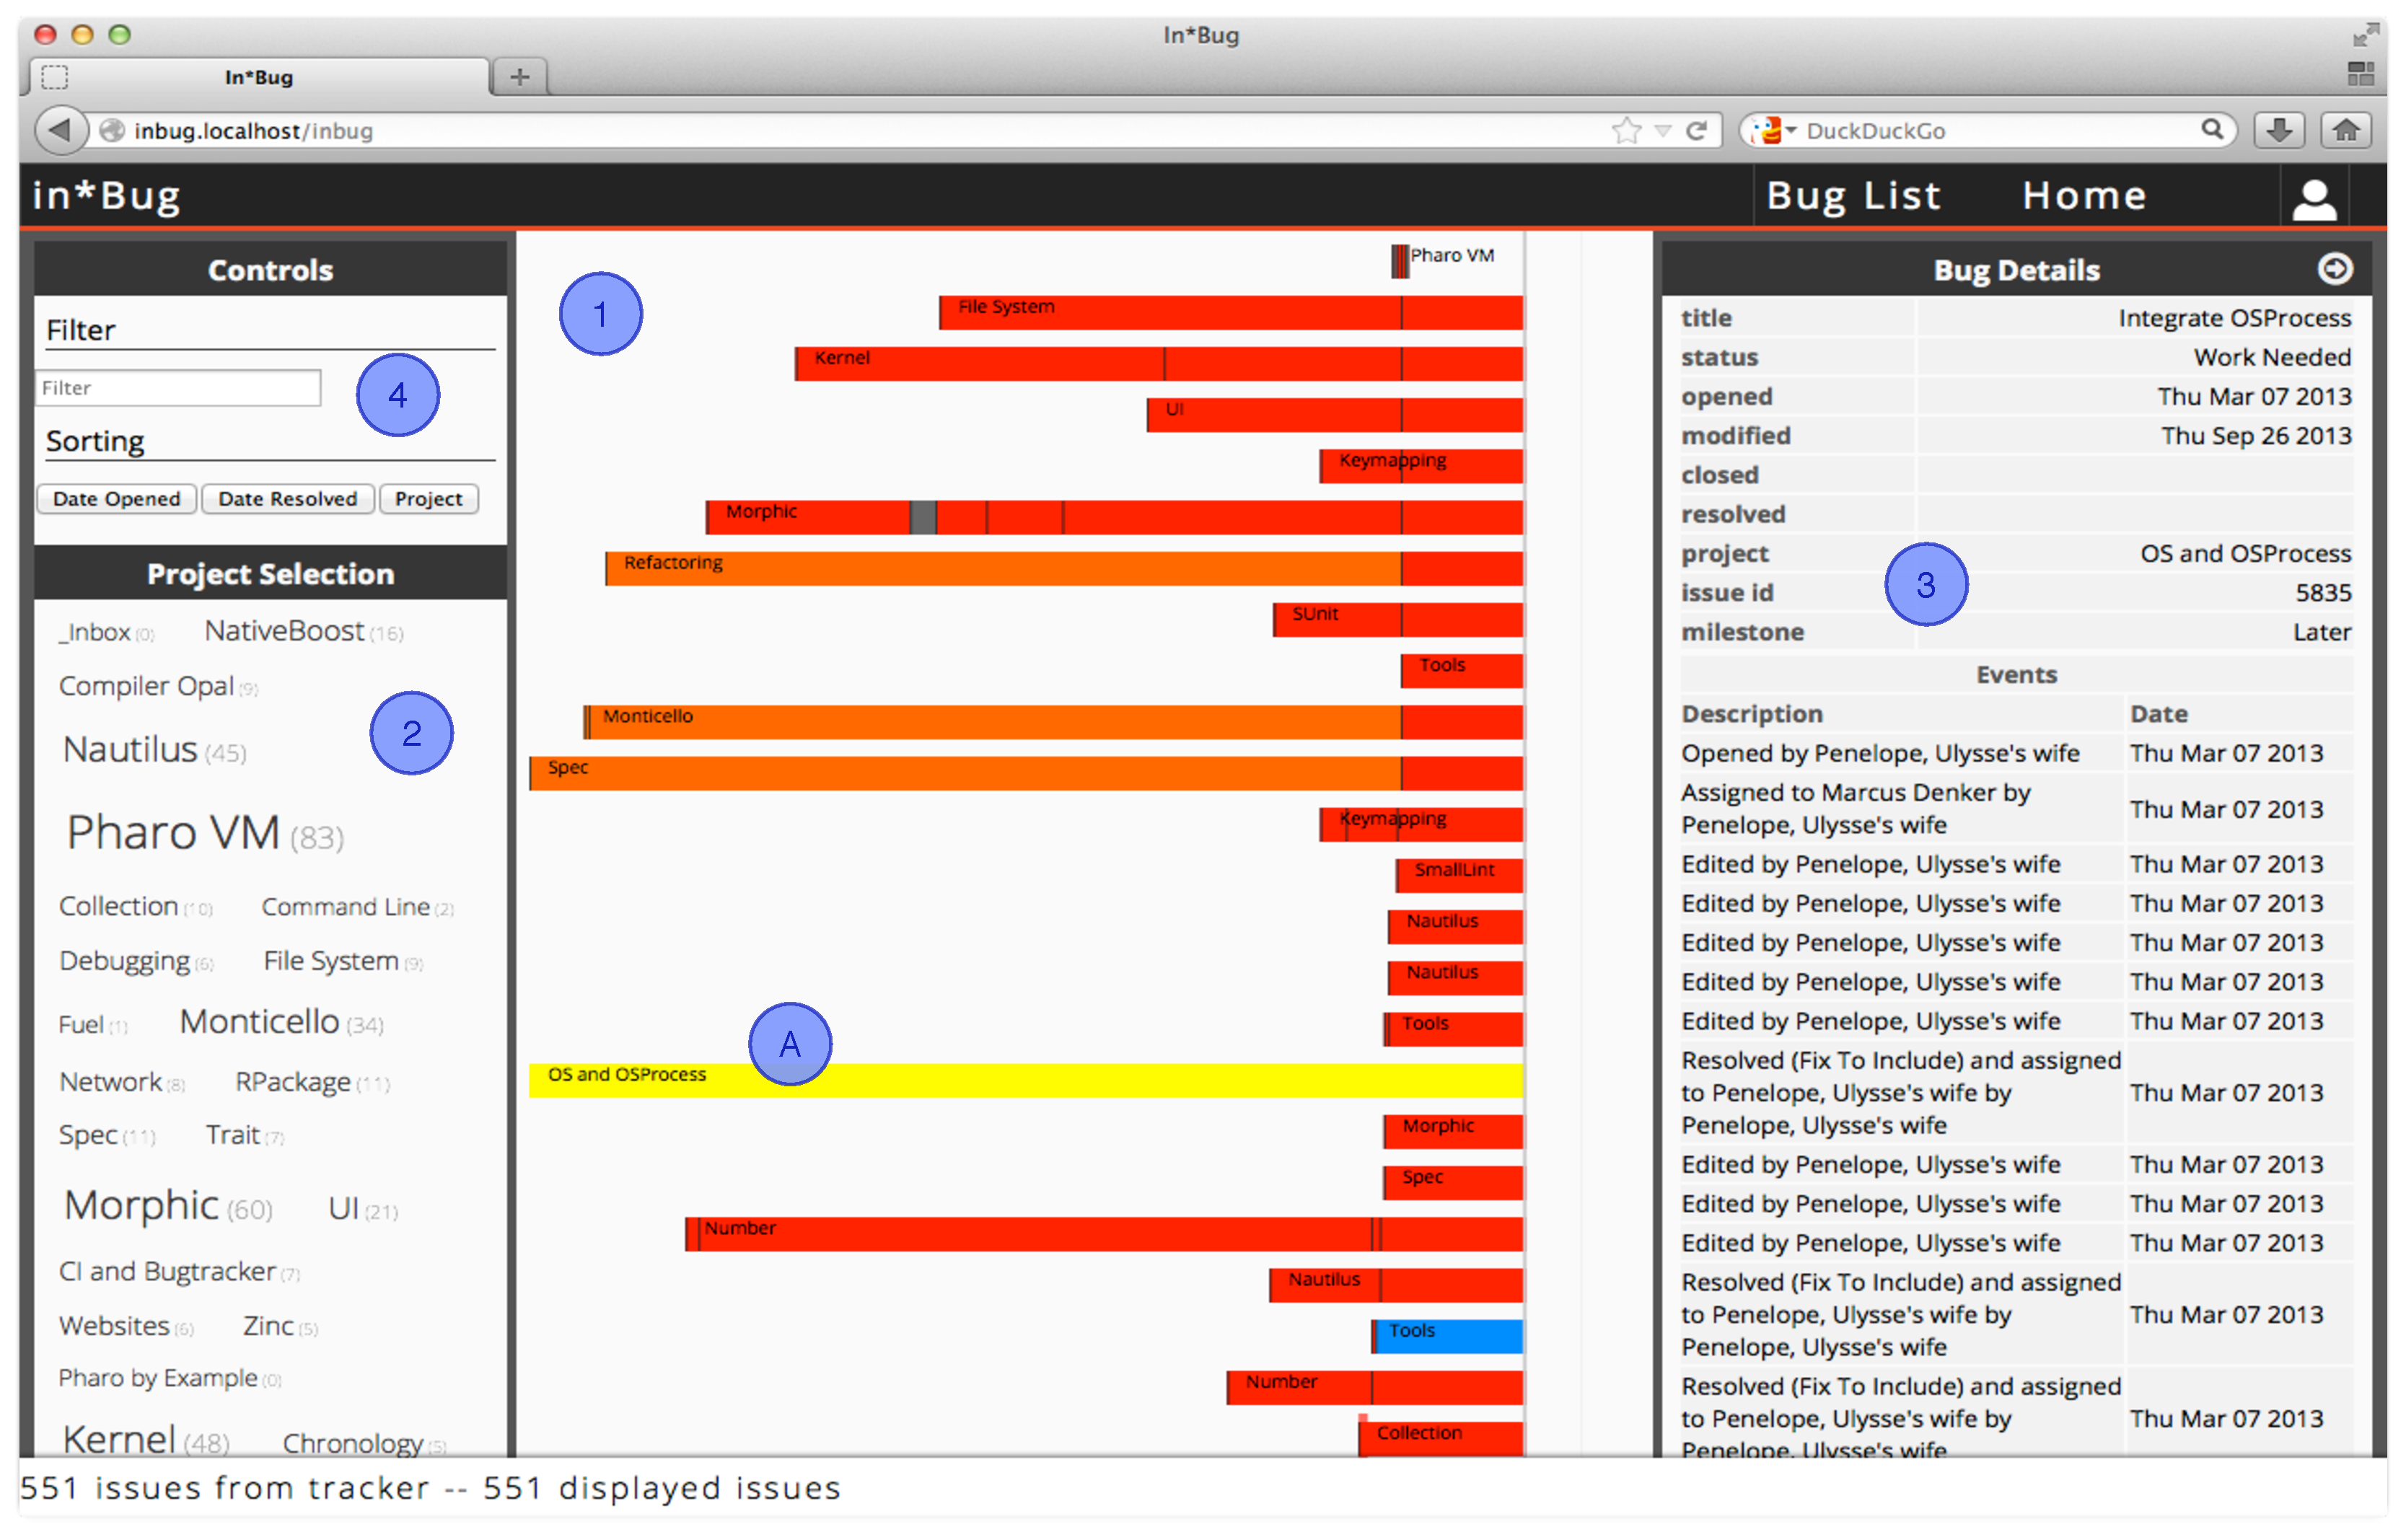
\includegraphics[width=\linewidth]{Images/visualize/inbug-list.pdf}
\caption{Main user interface of \ib}
\label{fig:inbug}
\end{figure*}

%%%%%%%%%%%%%%%%%%%%%%%%%%
\section{\ib in Detail}\label{sec:visualize-details}
%%%%%%%%%%%%%%%%%%%%%%%%%%

In this section we present the interface of \ib, detailing its panels and how we used the data in the issue tracking system to build the visualizations.

%%%%%%%%%%%%%%%%%%%%%%
\subsection{Main view}\label{main-view}

\figref{fig:inbug} depicts the main user interface, composed of the following panels:

\textbf{Bug lifetime panel (1).} \label{bug-lifetime-panel} This view depicts the bug reports contained in the bug repository, showing their duration (as a horizontal stacked bar chart) and status (using different colors, listed in \tabref{tab-colors}).

\begin{table}[ht]\small
\centering
\caption{Bug report event color codes}
\label{tab-colors}
\rowcolors{1}{tablefirstrow}{tablesecondrow}
\begin{tabular}{l p{0.1cm} l | l p{0.1cm} l } \hline
Active & \cellcolor{active} & orange & Work Needed & \cellcolor{work needed} & red \\
Closed & \cellcolor{closed} & gray & Resolved & \cellcolor{resolved} & dark gray \\
Working On & \cellcolor{working on} & blue & On Hold & \cellcolor{on hold} & cyan \\
Unknown & \cellcolor{unknown} & light grey & Selected & \cellcolor{yellow} & yellow \\ \hline
\end{tabular}
\end{table}

In \figref{fig:inbug} one specific bug (marked as A) is under focus.
The vertical line to the right indicates the current date, making it also clear whether a bug report is still active or not (if it is, it will touch that line).
This view also helps the developer to evaluate the complexity of a bug report by summarizing the events occurred during its lifetime.

\subsubsection{Project selection panel (2)}
In this panel the user can pick the projects whose bugs she is interested in.
All projects are shown as a tag cloud, where the tag size indicates the number of bugs reported for the project, also indicated with numbers between parentheses close to the name of the projects.

\subsubsection{Details panel (3)}
This panel provides all the information reported about the bug report under focus in the bug lifetime panel.
This panel present both the metadata and the list of events that happened during the lifetime of a bug, including description and date of each event.
The metadata is presented as extracted from the bug repository, \eg the opening date, the status, the last modification date, etc.

\subsubsection{Filter and options panel (4)}
This panel allows the user to sort and filter bugs.
The three default sorting criteria order the issues by project, opening date, or date in which the bug has been resolved.
The \textit{filter} field offers the possibility to enter either regular expressions or pieces of \emph{Smalltalk} code as queries, allowing the users to submit custom made queries to filter bugs.

%%%%%%%%%%%%%%%%%%%%%%%%%%%%%
\subsection{Details of a bug}

\begin{figure*}[ht]
\centering
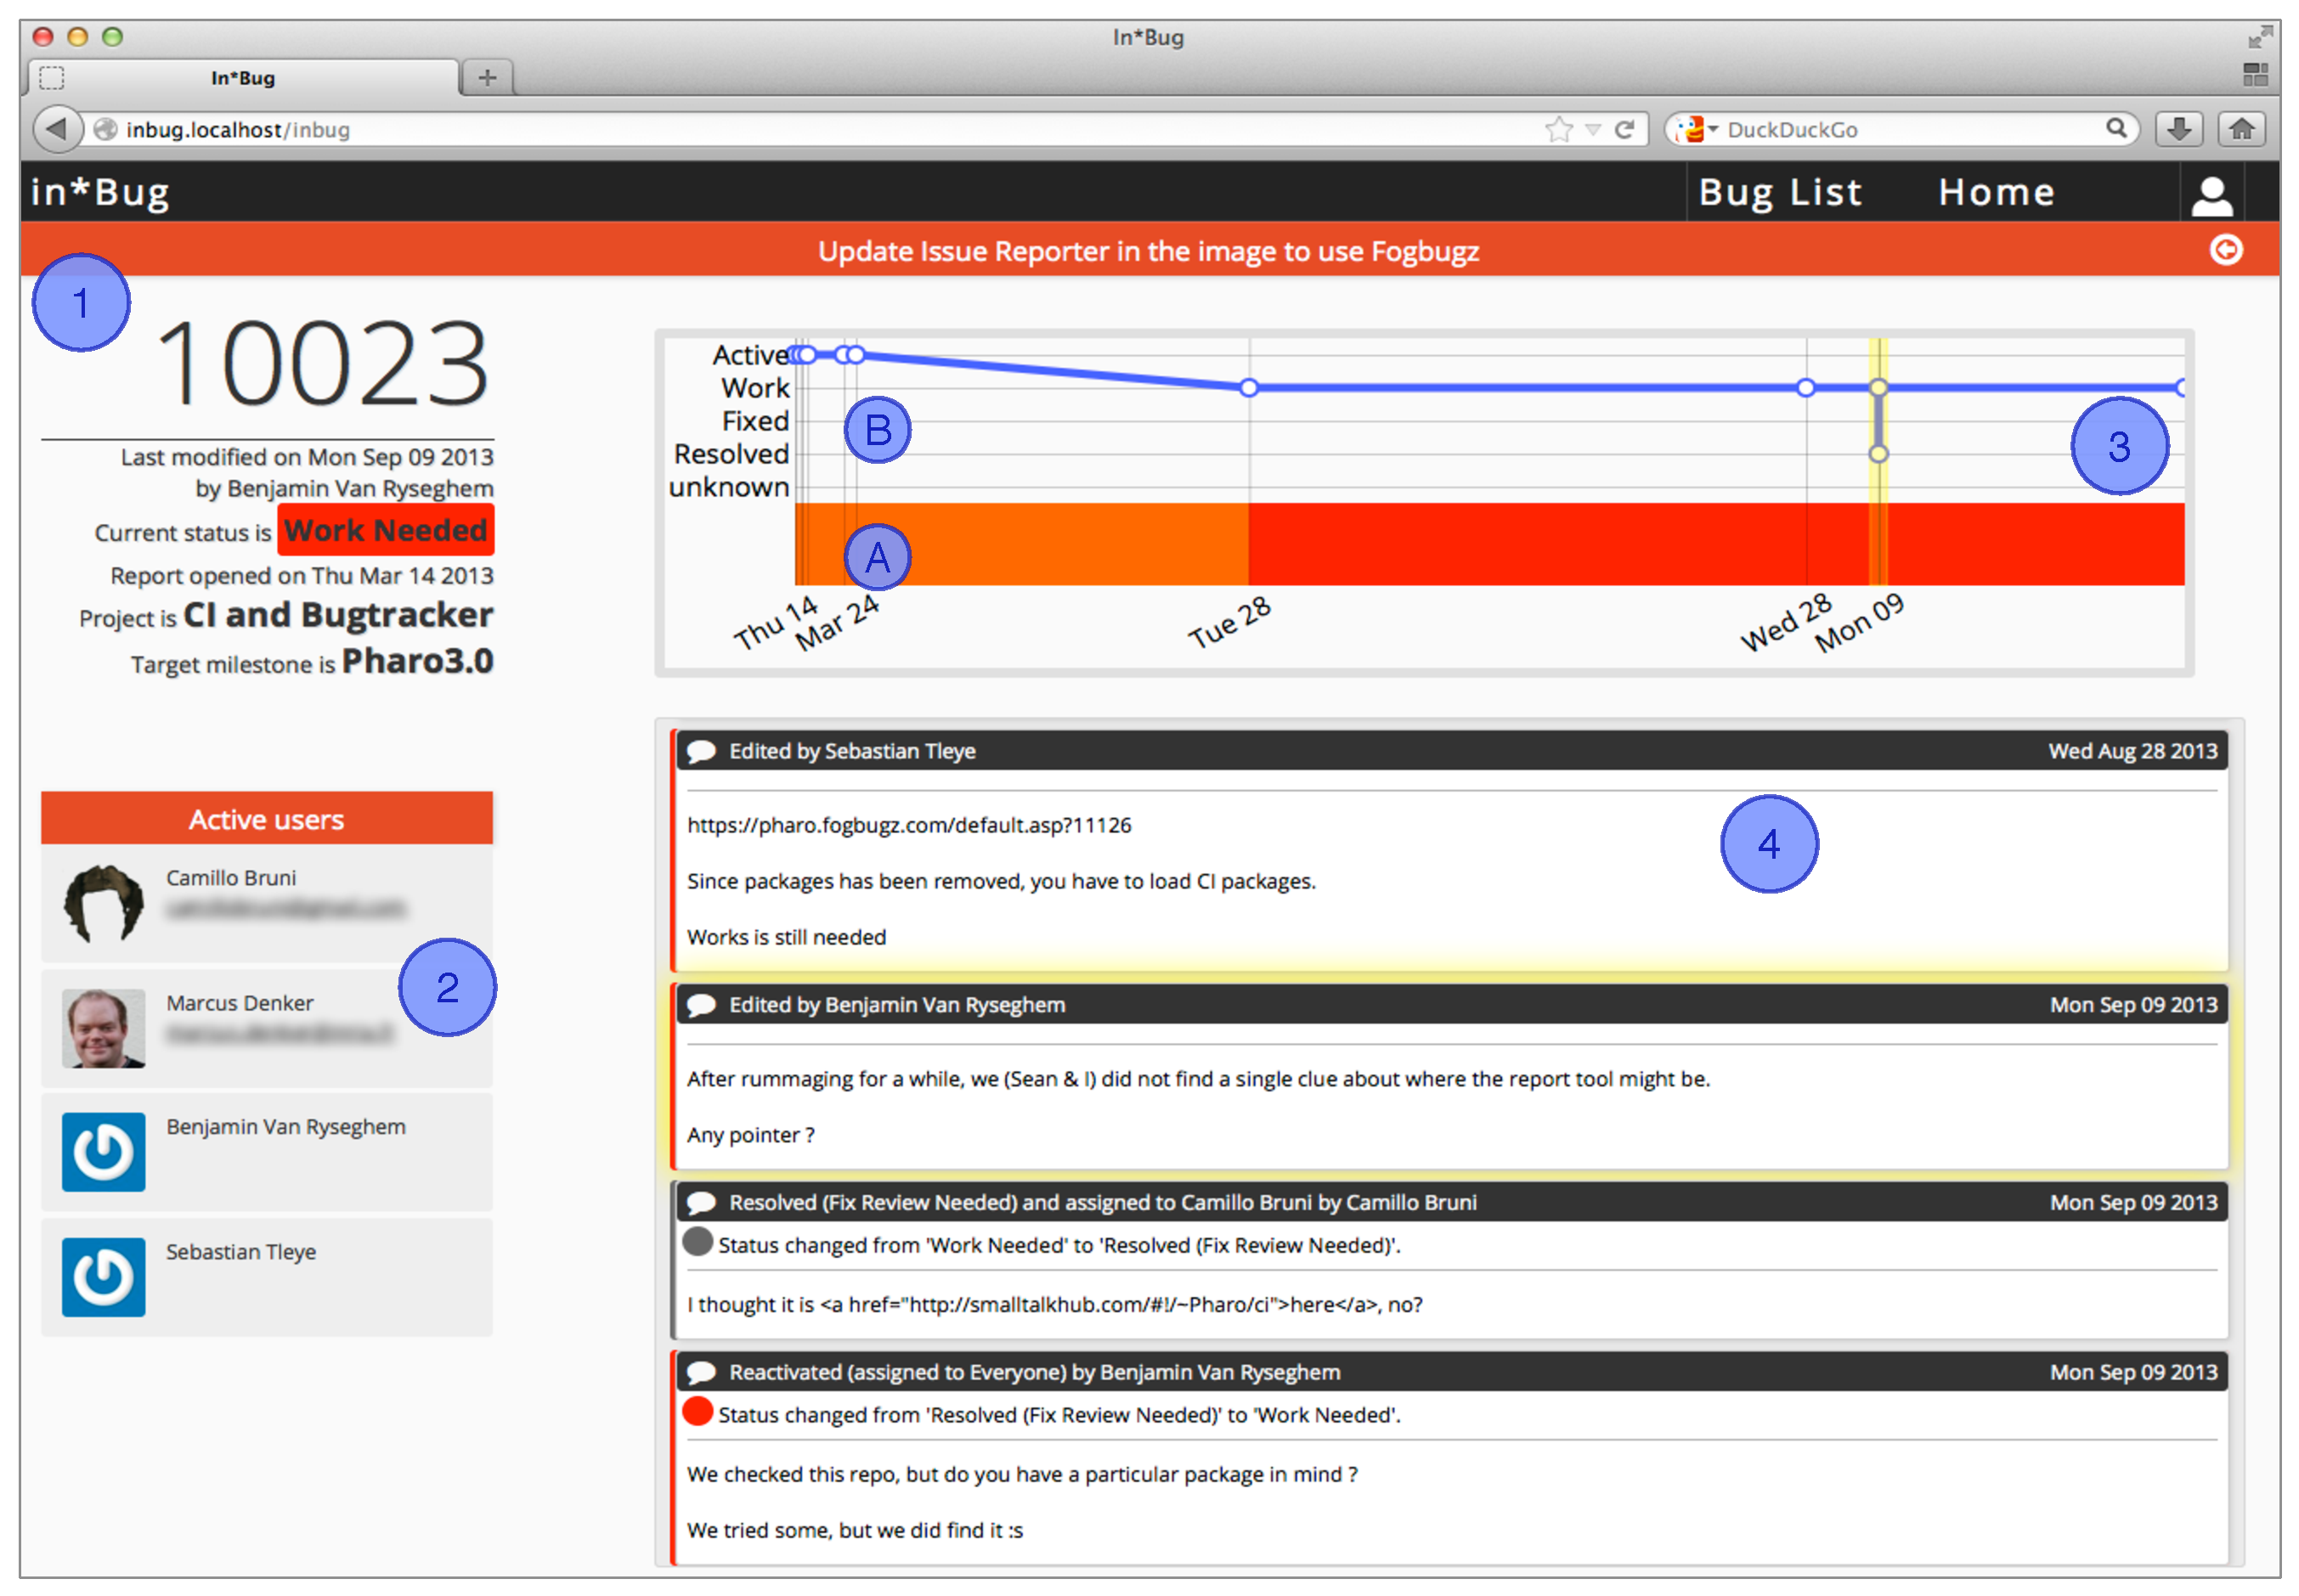
\includegraphics[width=\linewidth]{Images/visualize/details-page.pdf}
\caption{\ib details page showing the properties of a bug report}
\label{fig:inbug-home}
\end{figure*}

This view (see \figref{fig:inbug-home}) presents a detailed representation of a specific bug report.
Each section provides a description of the element that compose the description of a defect.


\subsubsection{Bug Report Metadata (1)}
The first panel summarizes the important metadata of the bug report: the id, the last modification, the current status, the opening date and possible closing date, the project and the target milestone for the issue resolution.

\subsubsection{Users List (2)}
This panel gives an overview of the people involved in the evolution of the bug.
In particular, the list displays the information of each user that performed an action on the issue, that was stored as an event.
The details include the picture of the user, the user name and the user's email address\footnote{We obfuscated the email addresses in the figure for privacy reasons.}, to contact the people working on an issue.

\subsubsection{Bug Report Life Visualization (3)}
This panel shows a visualization of the life of a bug report during time.
The left border represents the date the issue was opened, the right border represents the moment the bug was closed, or the current date if the bug report is still active.
The (A) section proposes the same visualization of the list view in the main view (\ref{main-view}), emphasizing the status changes during time.
The (B) section shows a line diagram where the height represents the criticality of the status (\ie fixed is the lowest and active is the hightest) and highlighting each event with a circle.

\begin{figure}[t]
\centering
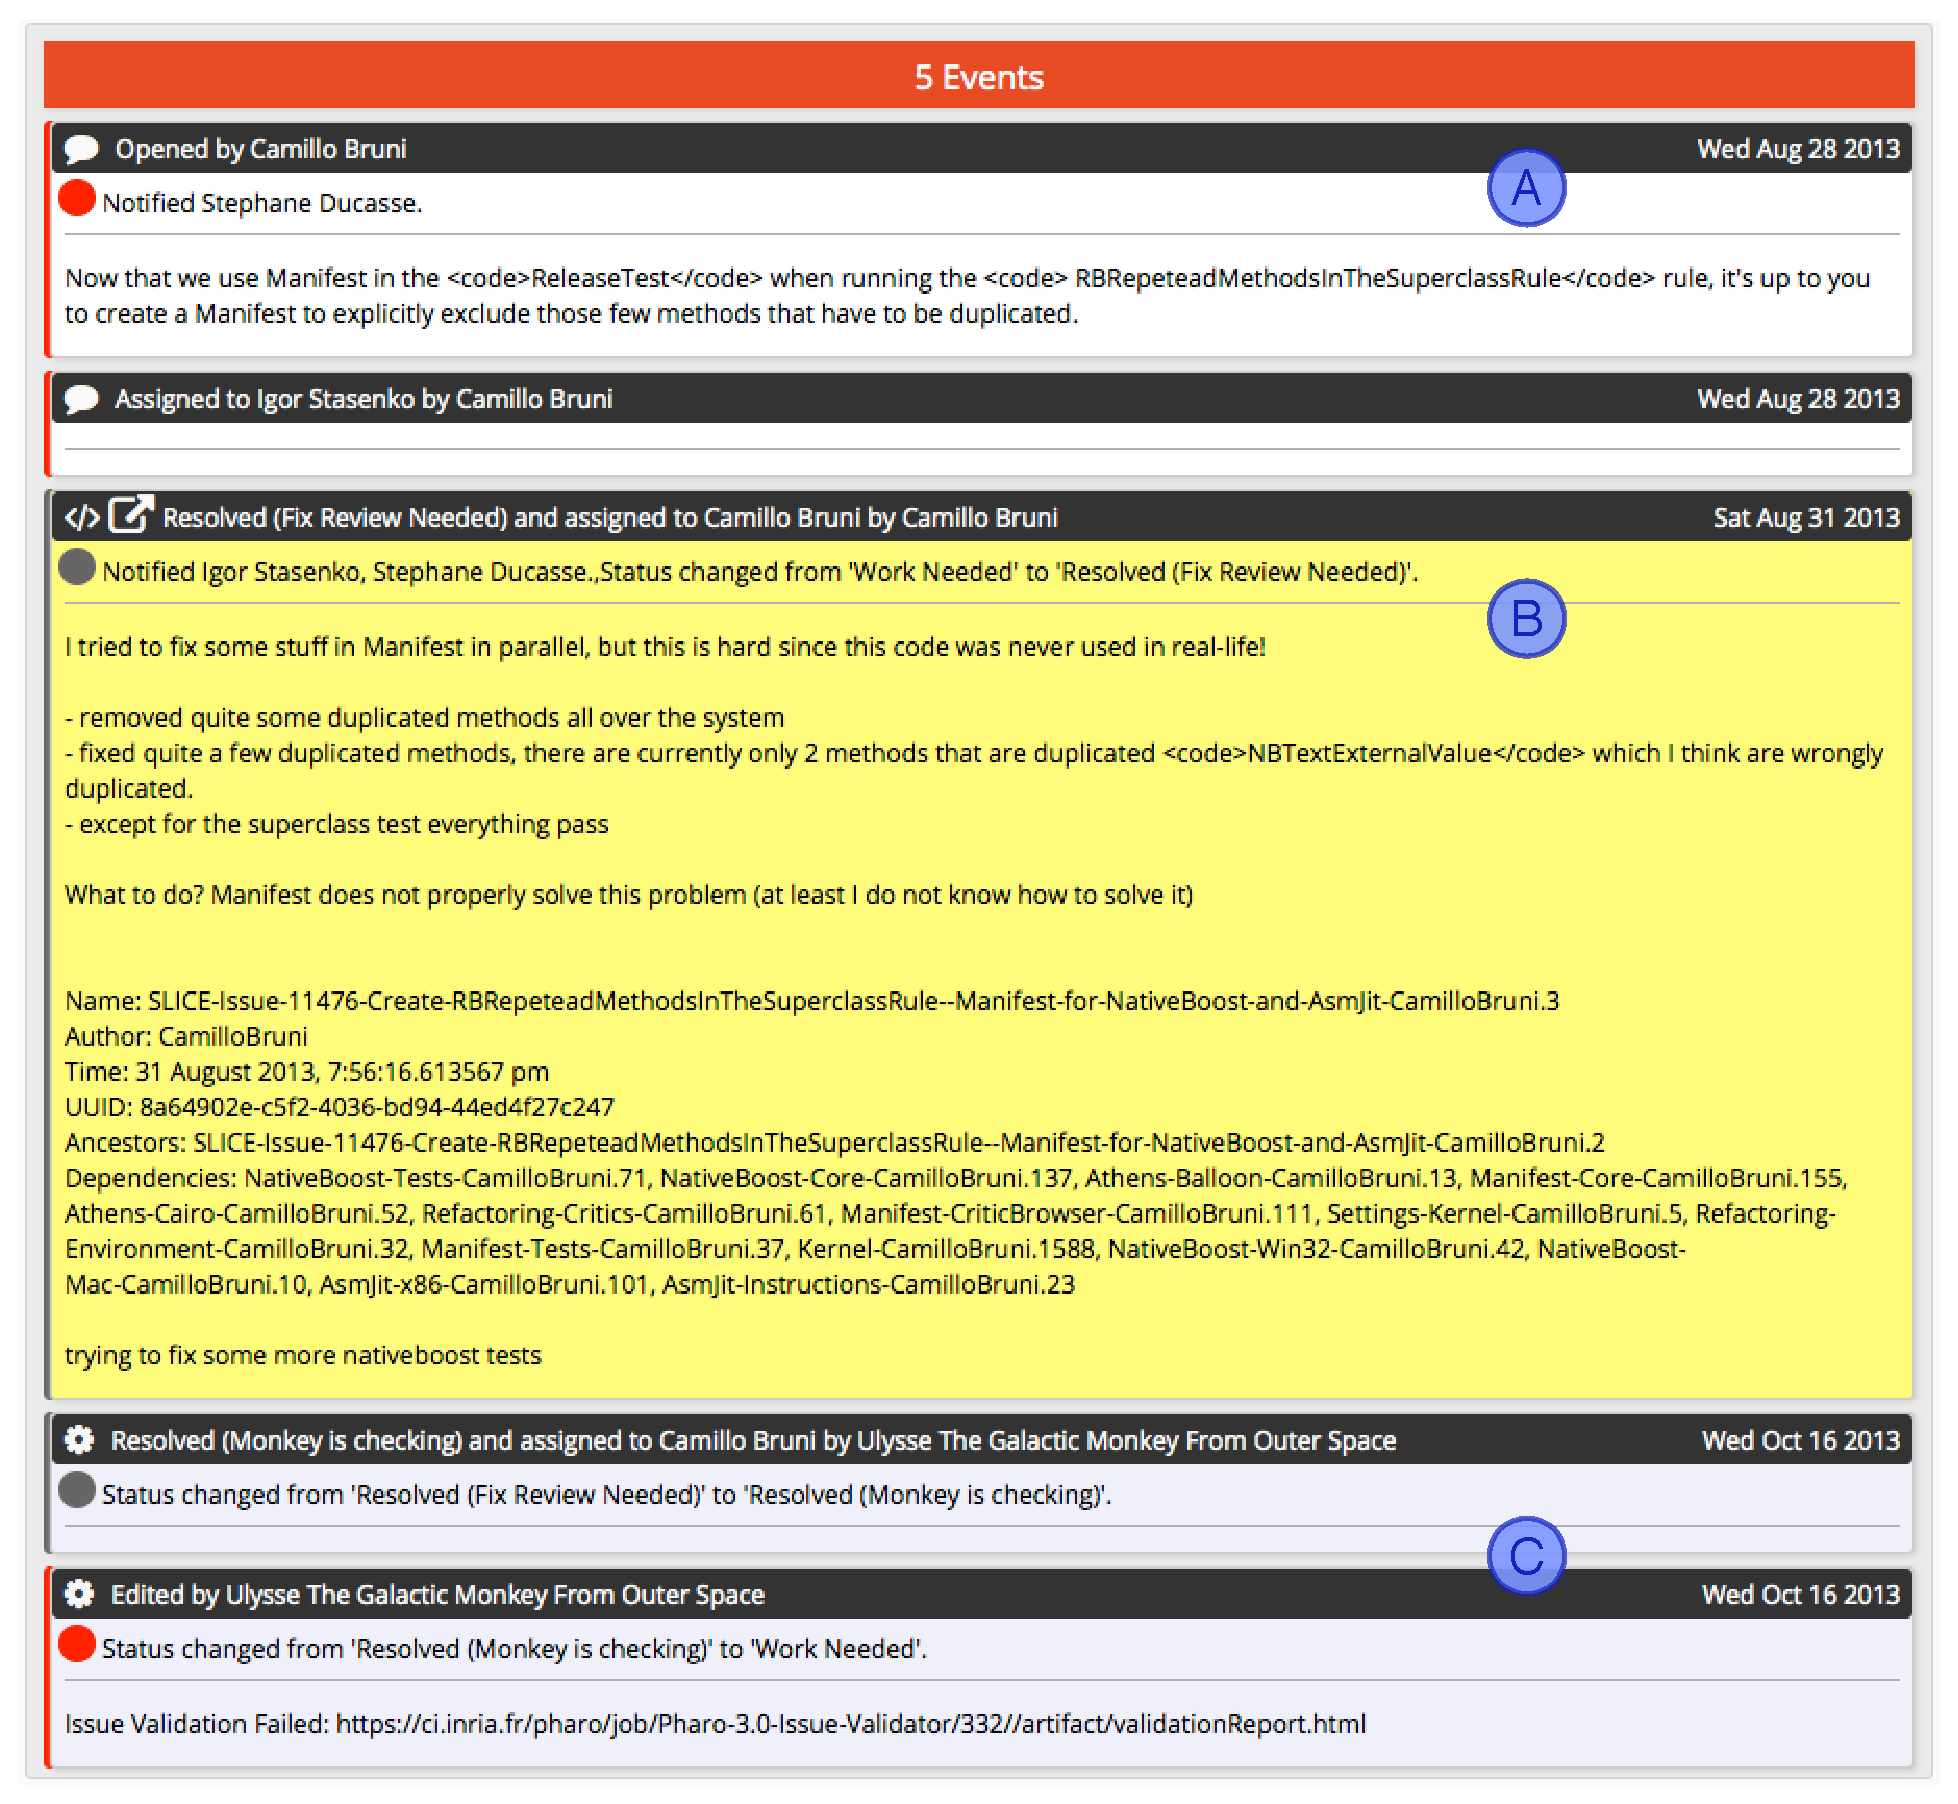
\includegraphics[width=.85\linewidth]{Images/visualize/event-list.pdf}
\caption{List of events in a bug report}
\label{fig:event-list}
\end{figure}

\subsubsection{Event Interactive View (4)}
This is a list of all the events that compose a bug report.
It shows the metadata of the event and whether it is an automatic event or an event generated by a user.
It also detects and highlights the patches of code submitted to the tracker for the issue resolution, and provides a link to download and inspect the patch.
The user can click on an event to highlight it both in the events list and in the bug report lifetime visualization.
\figref{fig:event-list} shows a detail of the event list, where we can observe the three types of events: (A) shows a comment by an user; (B) shows a submitted patch.
The upper left icon offers a link to the repository page of the patch; (C) indicates events automatically generated from bots in the tracker.
Inspired by more semantically rich and elaborated views, such as Ogawa et al's storylines~\cite{Ogaw2010a} or Kuhn and Stocker's storytelling timelines~\cite{Kuhn2012a}, the left border of each event is colored according to the status of the event, to help the user to keep track of the evolution of the bug while inspecting the list of events.

%%%%%%%%%%%%%%%%%%%%%%%%%%%%%%%%%%%%%%%%%%%%%%
\subsection{Implementation \& Current Dataset}

\ib is a web application built on top of the \pha environment.
It uses the \sea web framework~\cite{Duca2010a} to provide the data stored in a \textit{MongoDB} database and implements a \textit{RESTful API} to communicate with the client.
The client interface is implemented in \textit{JavaScript} using the data manipulation and visualization library \textit{D3.js}.\footnote{\url{http://d3js.org/}}

\ib is built to visualize the \fbz repository of the Pharo ecosystem.
In \tabref{tab:tracker-summary} we provide a summary of the data we investigated.

\begin{table}[ht]\small
\centering
\caption{Summary data of the \textit{Pharo} bug tracker}
\label{tab:tracker-summary}
\rowcolors{1}{tablefirstrow}{tablesecondrow}
\begin{tabular}{p{7cm} r} \hline
Number of projects & 46 \\
Number of bug reports & 8,666 \\
Number of open bug reports & 613 \\
Total number of events & 79,437 \\
Average events per issue & 9 \\ \hline
\end{tabular}
\end{table}

\ib also provides links to patches on \emph{SmalltalkHub}, a source code repository to store versioned Smalltalk code.
In \figref{fig:inbug-ecosystem} we can see how these three services interact.

\begin{figure}[t]
\centering
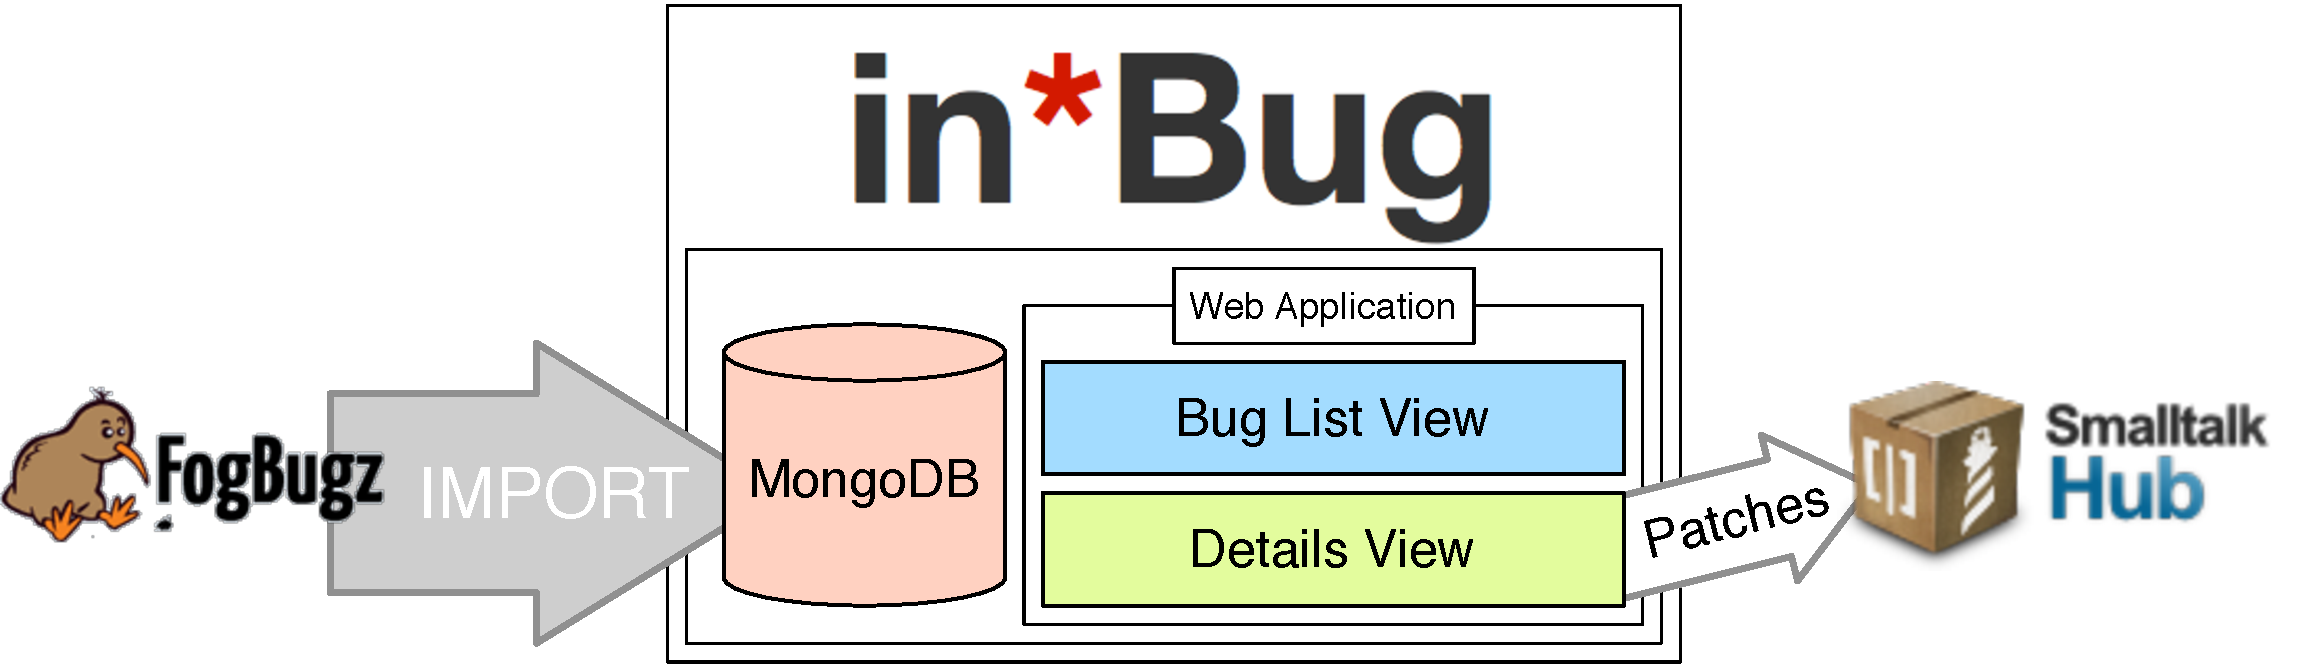
\includegraphics[width=.8\linewidth]{Images/visualize/inbug-ecosystem.pdf}
\caption{The interactions of \ib with the \emph{FogBugz} and \emph{SmalltalkHub} services}
\label{fig:inbug-ecosystem}
\end{figure}

%\pagebreak

The bug reports data is imported from FogBugz and stored in the MongoDB repository.
The web application then loads the data and present it in the list view of the main interface.
The details of a single report are presented in the details view, where the user can follow a link that leads to a patch submitted to SmalltalkHub.
%\input{application.tex}


\section{More Than Meets the Eye}

While developing \ib we verified that providing a visual feedback using data that is usually consumed through plain text is an effective method to observe and investigate properties that would normally be hard to isolate.
For example, in \figref{fig:inbug} we can easily separate the bug reports that are older from the newer ones, observe the amount of activity happening on an issue, spot cases where a bug report was reopened several times, or identify abandoned reports.
This experience convinced us that the textual representation we currently use in modern issue tracking systems is limiting the amount of information that we can obtain from the data we collect.


\newpage
%%%%%%%%%%%%%%%%%%%%
\section{Outline}\label{sec:visualize-summary}
%%%%%%%%%%%%%%%%%%%%

In this chapter we presented \ib, a web-based visual analytics platform to explore the content of a bug repository.
\ib allows to get a complete overview of a whole repository, as well as detailed and meaningful information on a single bug report, either through visualizations that allow to interact with the data, or with the query engine embedded in \ib that allows the user to submit queries and dialog directly with the bug reports.

% We intend to provide further visualizations that describe the resume data of a single bug repository, to ease and improve the comprehension of the evolution of a software project during time.

Since we designed \ib as a tool for practical development, we focused on the Pharo platform and we targeted its community.
However, the approach of \ib is general and therefore it can be applied to any bug tracking system.
%We plan to improve \ib and refine the existing visualizations based on feedback obtained from Pharo users.

%Our main target is the \textit{Pharo} community, as we want to propose \ib as a tool for developing the \textit{Pharo} platform and refine the existing visualizations and improve \ib based on feedback we will get from Pharo users.

% \subsection{The Road So Far...}
We saw that existing bug repositories contain information that can be highlighted using means other that plain text.
The underlying information we display, however, is still in textual form, with the consequence that we have to rely on the expertise of the user to obtain useful information.
We therefore decided to tackle the problem of the reliability of the data by means of automatic data collection during a software failure.
In the next chapter we present our approach to crowd-driven data collection: We collect and investigate a large amount of stack traces generated during development activities, to provide automated and reliable feedback to users and developers.


%\begin{figure*}[ht]
%\centering
%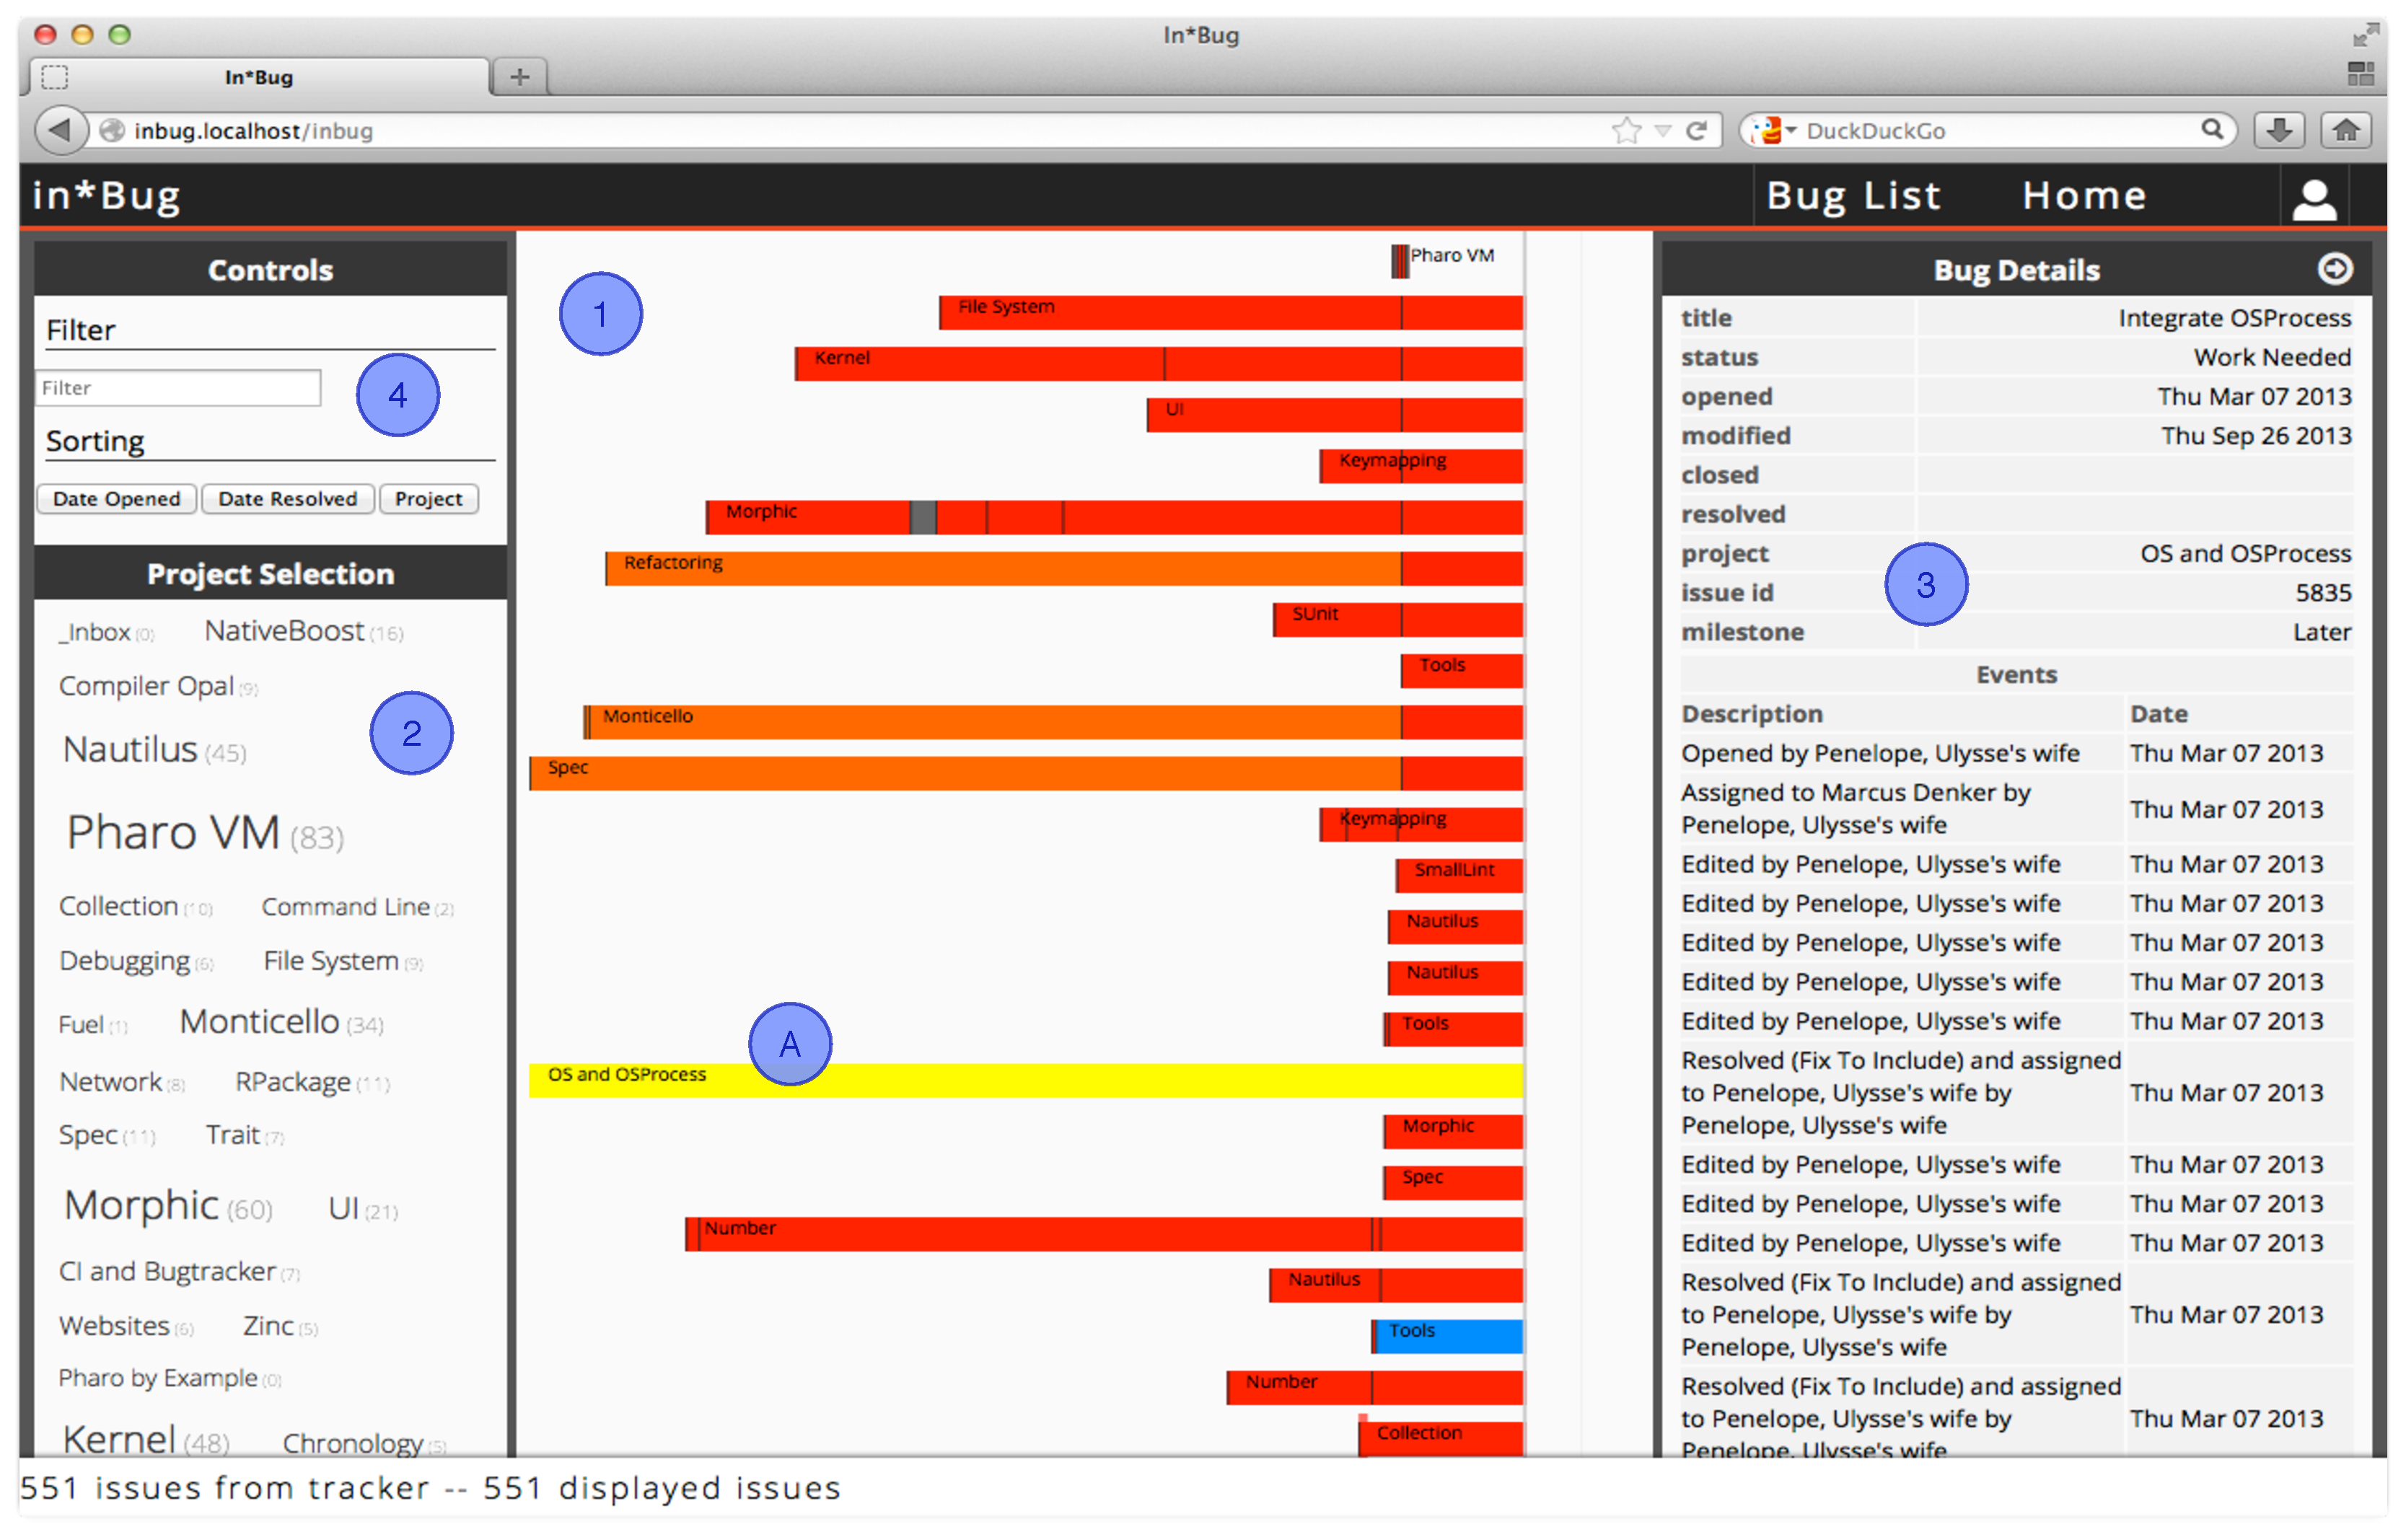
\includegraphics[width=\linewidth]{Images/visualize/inbug-list.pdf}
%\caption{Main user interface of \ib}
%\label{appendix-inbug}
%\end{figure*}

% \begin{figure*}[ht]
% \centering
% 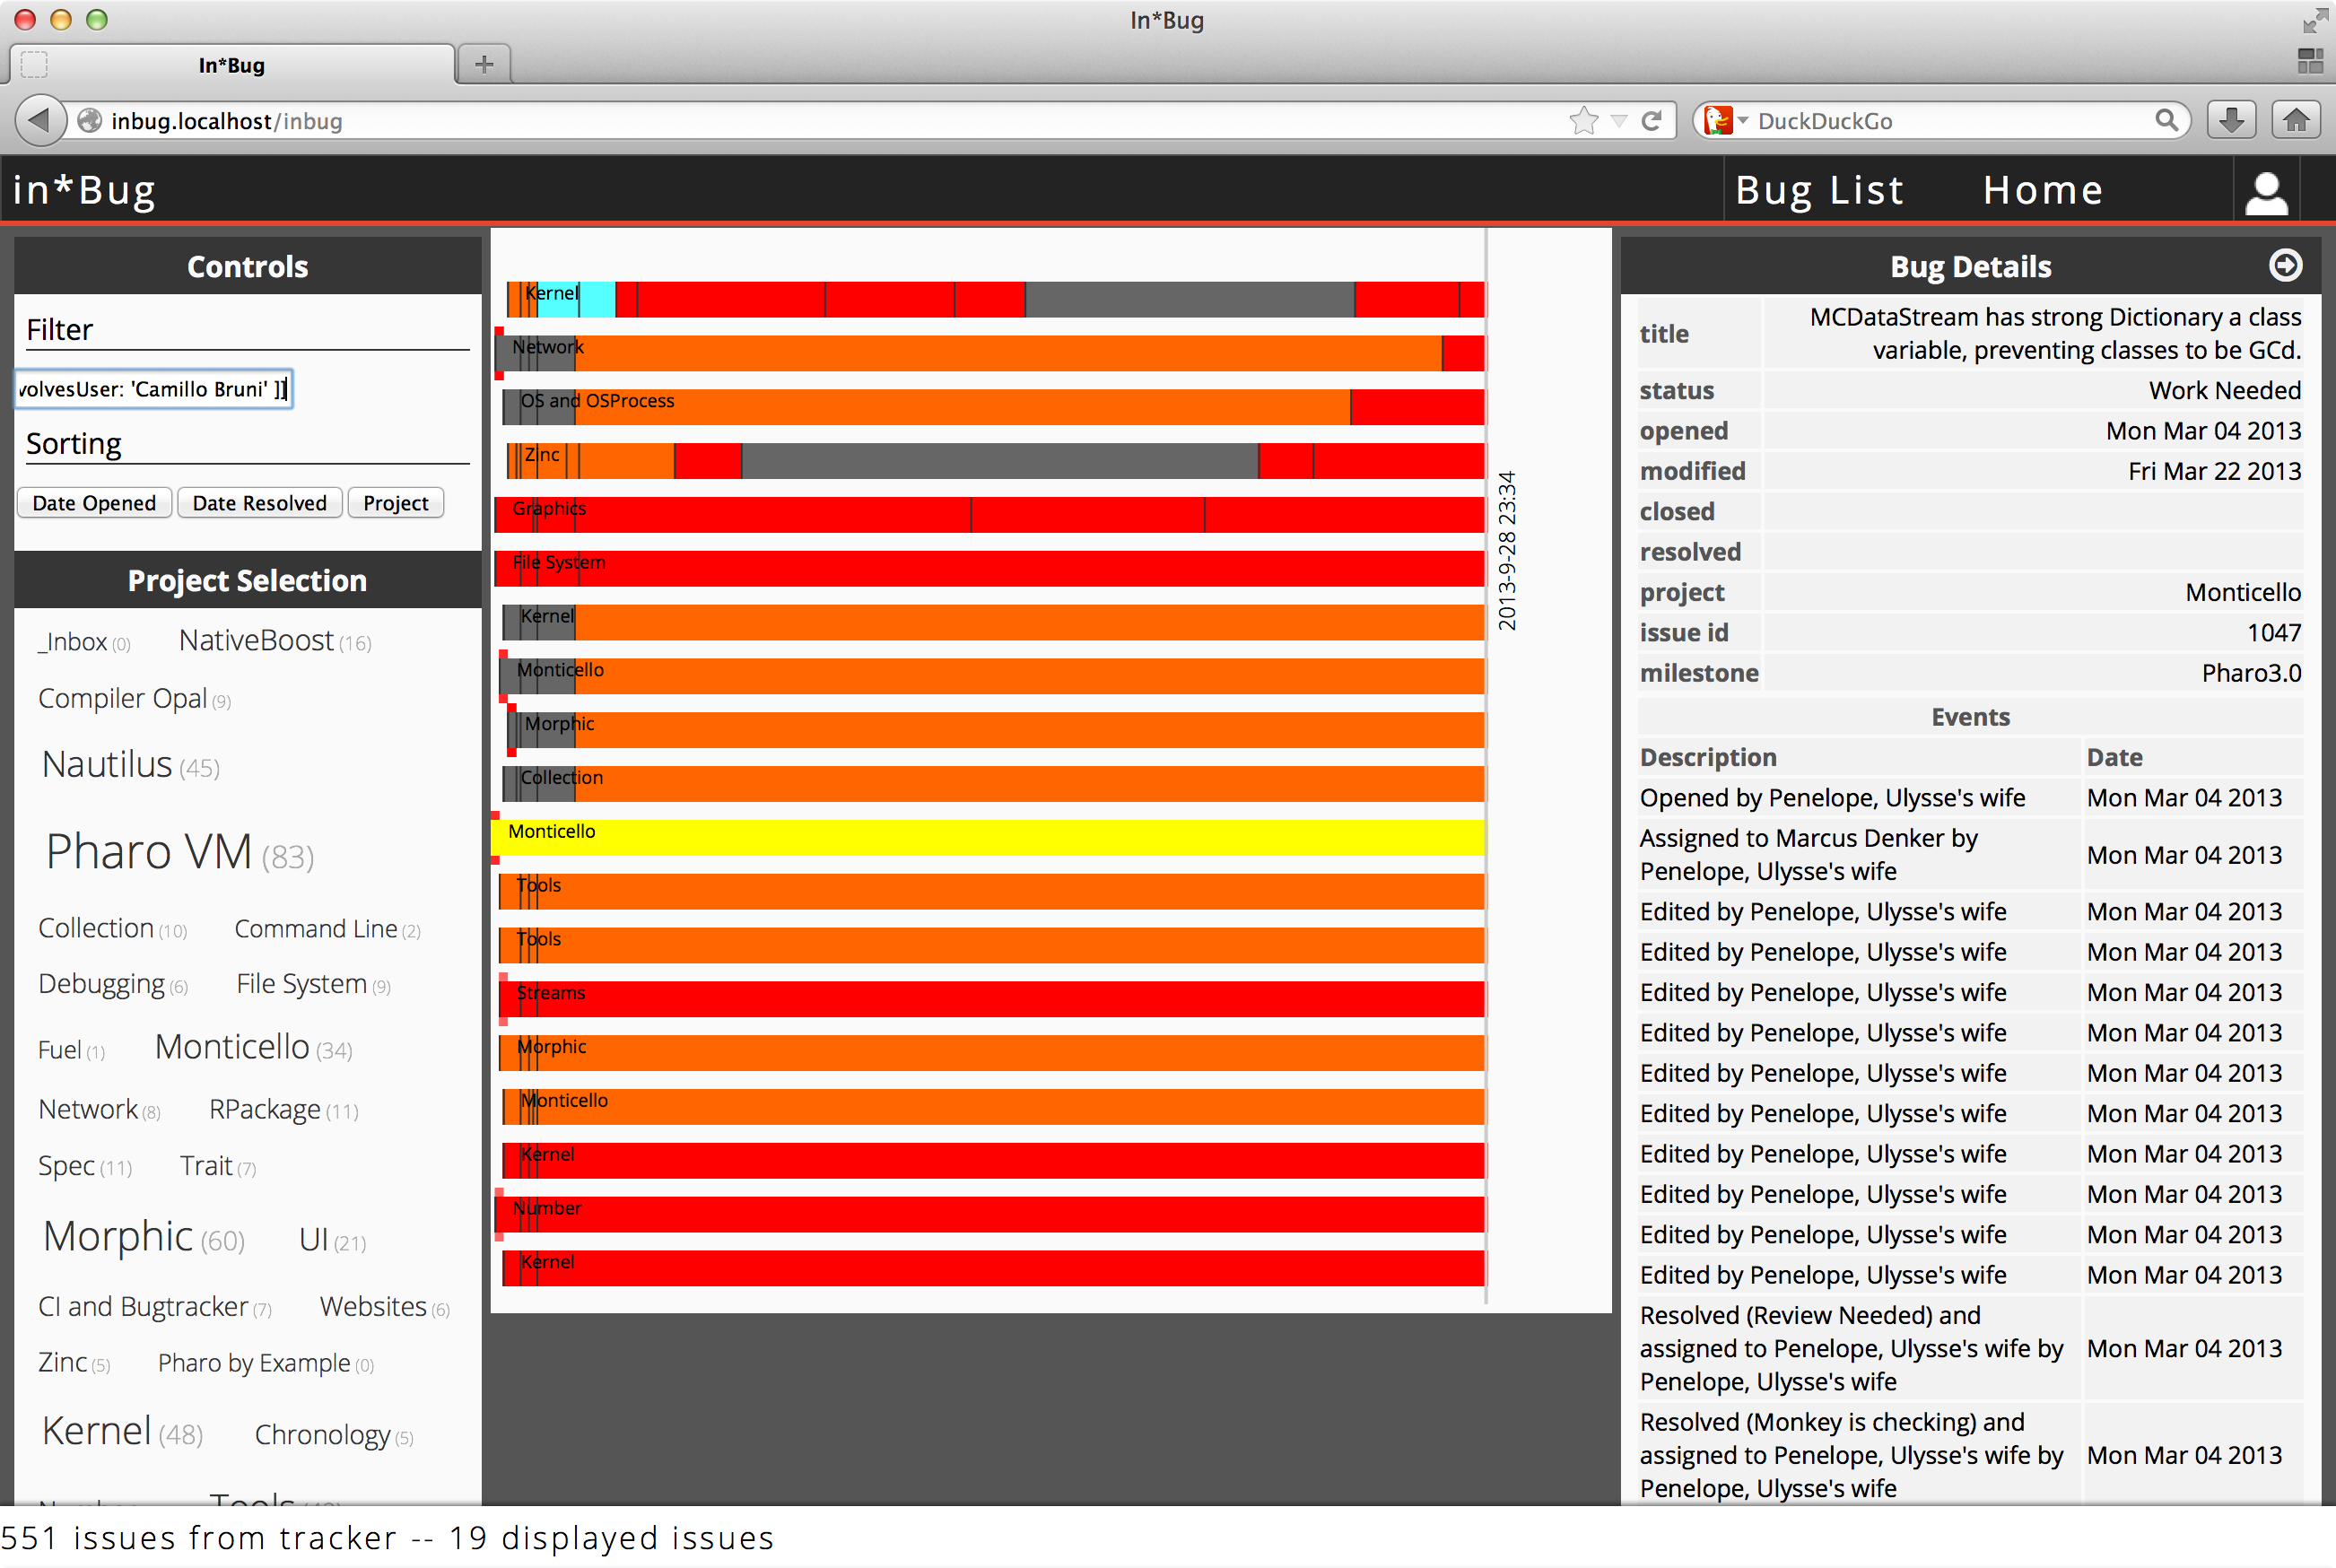
\includegraphics[width=\textwidth]{Images/visualize/appendix-query.png}
% \caption{The result  of a Smalltalk query}
% \label{appendix-query}
% \end{figure*}


% \section*{Appendix - Description of the demo}
%
% We foresee a very interactive demo, where in front of the audience we would use \ib to navigate the bug repository mentioned in \tabref{tab:tracker-summary}. In the following we do provide a plausible demo scenario, but would much rather prefer to have the audience give input on which bugs we would analyze together with them.
%
% \begin{enumerate}
%
% \item \textbf{Bug List View.} The beginning of the demo is to present the concepts behind the main interface of \ib. We are going to introduce the idea of a bug report as an independent entity and describe the visual representation chosen to describe a report. We then describe purpose of each panel, starting from the bug list: the possibility to examine a set of issues and their relation in terms of time collocation (see \figref{fig:inbug}).
%
% \item \textbf{Bug report manipulation filters.} We will show the capabilities of \ib to sort and filter the interesting reports. We will show an example of query submitted in Smalltalk, and show how we can find an interesting report with a visual inspection. \figref{appendix-query} shows the result of the query:
%
% \begin{verbatim}
% [ :each | each events size > 20 and: [
%   each involvesUser: 'Camillo Bruni' ]]
% \end{verbatim}
%
% \item \textbf{Details View.} We will select a bug report to inspect and visualize its properties with the details view presented in \figref{appendix-details-view}. We will present the metadata displayed, the users involved in the report resolution, then we will see how the visualization can provide an immediate feedback on the life of a bug report, and its current status.
%
% \begin{figure}[ht]
% 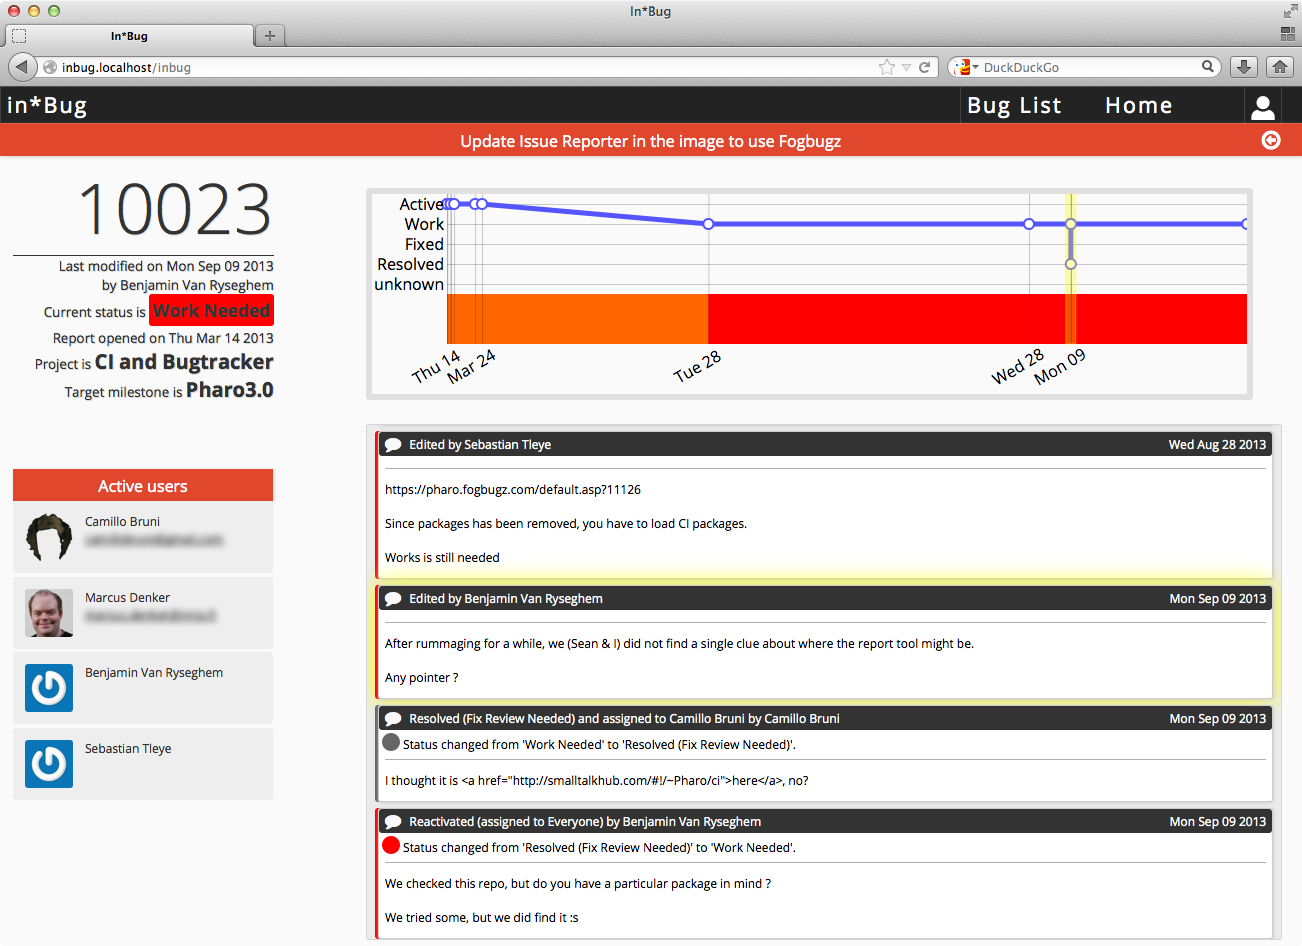
\includegraphics[width=\linewidth]{Images/visualize/details-page.png}
% \caption{\ib details page showing the properties of a bug report}
% \label{appendix-details-view}
% \end{figure}
%
% \item \textbf{Events and Patches.} We will examine the list of the events and the possible types of events described. We will show when \ib can detect if an event is a user comment, an automatic event or a patch submitted to fix the problem. We will show how \ib provides a link to directly retrieve the patch and examine it.
%
% \end{enumerate}
%
% We plan to wrap up by having a discussion about other extensions we are currently implementing, and showing off some of the directions we are currently pursuing.

  %!TEX root = ../tommaso-thesis.tex
%!TEX spellcheck = en_US


\chapter[Multi-concern Visualization of Large Software Systems]{Multi-concern Visualization of \\Large Software Systems}\label{ch:blend}
% \coolchapter{Blended, Not Stirred}{Multi-concern Visualization of Large Software Systems}{ch:blend}

While constructing and evolving software systems, developers generate directly and indirectly a large amount of data of diverse nature, such as source code changes, bug tracking information, IDE interactions, stack traces, etc.
Often these diverse data sources are processed and visualized in isolation, leading to a partial view of systems.


In the previous chapters we saw that we can collect data from runtime errors and use this data to get insights into the development process.
In this chapter we present a \emph{blended} approach to visualize several data sources.
We combine these ``ingredients'' at once, to give as complete an answer as possible to the question \emph{``What happened to the system in the last few days?''}.
The goal is to enable a quick and comprehensive assessment of what happened to a software system in any given time frame.

\structure

% \secref{sec:blend-related} presents the related work.
In \secref{sec:blend-ingredients} we describe the ingredients of our blended visualization, which is presented in \secref{sec:blend-visualization}.
In \secref{sec:blend-stories} we use the visualization to tell interesting evolutionary stories.
\secref{sec:blend-discussion} discusses possible extension to our approach.
Finally, \secref{sec:blend-summary} summarizes and concludes the chapters.

\newpage


%%%%%%%%%%%%%%%%%%%%%%
\section{Exploring a System} \label{sec:blend-intro}
%%%%%%%%%%%%%%%%%%%%%%

Software development involves a variety of activities carried out with a number of tools, components and environments, that relate to many different aspects of a system.
The increasing size of software projects, the increasing popularity of distributed development platforms like \texttt{GitHub}\seeurl{https://github.com}, and the amount of tools and frameworks available for every language, turned a significant part of modern software development into an integration process, where the developer can define a behavior by orchestrating and specializing library components and third-party entities.
This has turned the engineering of any software system into an information-heavy process, which is ultimately distilled into (hopefully functional) source code.
The vast majority of the corollary information (such as discussions, design decisions, email communication between developers, bug reports, etc.) is either discarded or ignored.
This is in part due to its often only semi-structured nature, where structured fragments are interleaved with natural language.
The mining of such unstructured data has become a research field of its own in the past few years.

When it comes to the understanding of any system, the natural focus is the source code, and indeed it --and the overarching structure and architecture-- has been the primary subject of study of program comprehension research.
In the context of software visualization many approaches have been developed to visualize the (evolving) structure of software systems, which range from static visualizations to historical or dynamic ones.
What strikes in this context is that many approaches consider only single concerns, such as the architecture, the structure, the evolution, the relationships, etc., but there is little in terms of visualizing multiple concerns at once.

We present here an approach to visualize multiple concerns concurrently.
The concerns we tackle are interaction data, failure information, and evolution.
Interaction data stems from how developers interact with the integrated development environment (IDE) while developing and maintaining a system.
In essence, it provides evidence of where and how people have been active while developing~\cite{Mine2015b}.
Failure information is generated each time the debugger is triggered because an exception has been raised.
In our previous work we have shown that such data can be leveraged to understand where the particularly tricky spots in a software system are located~\cite{DalS2015a}.
Both interaction data and failure data are more fine-grained than their respective counterparts, namely versioning information and bug reports.
We complement these two types of data with a third one, the evolution of the system.

Although we focus on these types of information, our approach can be extended to feature any kind of information artifact related to a large software system under development.
In essence, our goal is to answer one of the most often asked questions raised by developers and managers alike, namely ``what happened to our system recently''?~\cite{Sill2008}

We present a visual approach to \emph{blend} development data originating from different  sources, \eg by different tools that record and persist code changes, interaction data and stack traces.
We propose an interactive map that summarizes the relevant events that involved the system in a given period of time, using the city metaphor to represent a software system~\cite{Wett2007}, and coloring each entity according to the combination of data gathered around it.
We allow to explore the evolution of the system by navigating the information during time, and refining the search of interesting events to specific moments.
We then present some stories obtained through our visualization that illustrate interesting properties of an existing software project and its community.

The contributions we present in this chapter are:

\begin{itemize}

\item A novel approach to visualize multiple concerns concurrently in large scale software systems.

\item The supporting tool infrastructure to mine and integrate the data stemming from various sources of information.

\item Initial anecdotal evidence that our approach indeed allows us to discover and investigate facts that would otherwise remain hidden in the literal ``sea of data'' that surrounds any large and long-lived software system.

\end{itemize}


% \section{Related Work}\label{sec:blend-related}
%
% Many researchers showed how using data generated during the programming activity can provide valuable information about the evolution of a project.
%
% For example, Bacchelli et al.
% proposed an Eclipse plugin to integrate email communication in the IDE~\cite{Bacc2011a}.
% They showed that having the email data produced during the development of a software system at one's disposal helps supporting program comprehension tasks, such as finding entry points in a system and recovering additional documentation.
% %For example, Bacchelli \etal proposed a popularity metric based on the volume of discussion generated by software entities in development mailing lists, and showed that this information, correlated with source code and change metrics, helps in improving the predictive powers of defect prediction techniques~\cite{Bacc2011a}.
% Another example has been given by Zimmermann \etal, who applied data mining techniques to version histories to detect changes and build prediction model to suggest future changes to developers~\cite{Zimm2004a}.
%
% To effectively present and understand such an amount of data, many researchers and practitioners are adopting visualization and \emph{Visual Storytelling} approaches.
% The ability of contextualizing the information in a story that explains the meaning of the data is becoming more and more central to the skills required to data scientists~\cite{Segel2010a}.
%
% Among the different visualizations that researchers used to represent a software system, the city metaphor has proven to be effective in giving a high level picture of a group of entities, allowing the user to navigate, zoom and inspect the various components and refine the view~\cite{Wett2011a}.
% This approach has been adopted in different scenarios, depicting different kind of information pertaining several steps of the development activity, such as changes in the system, the defects involving different components in the system, issues in quality checking rules or the exceptions in the system~\cite{Panas2003a}.
%
% Other visualization approaches tried to focus on the evolution of software systems, specifically the version repositories, the dependencies or the structures.
% For example, Fischer \etal~\cite{Fisch2006a} proposed EvoGraph, an approach based on data extracted from a system release history, that visualizes the evolution of structural dependencies through 2D visual representations.
% Girba \etal~\cite{Girb2005a} focused on the visualization of the evolution of class hierarchies, correlating the history of classes and their relationships, \eg inheritance.
% The approach by Voinea \etal~\cite{Voin2007a} uses a combination of color and texture to represent as many attributes as possible to display information extracted from software configuration management systems.
% Another important approach is the one by Ratzinger \etal~\cite{Ratz2005a}, that represents systems as nested, zoomable graphs.
%
% However, while these approaches effectively visualize data about a single aspect that impacts or involves a system, they fall short in correlating this information with knowledge coming from diverse data sources and impacting diverse concerns.
% Such additional information could effectively integrate the existing data to uncover further relations between the elements of the system.
%
% We think that an approach that considers more than one kind of data and presents the information in a unified, uniform view, normalizing and balancing each source, could provide a greater value in understanding a software project and the activities happening in its ecosystem.



\section{The Ingredients}\label{sec:blend-ingredients}

%As per the title of our paper, \emph{``Blended, Not Stirred''} our visualization presents a blend of different ingredients to enable analysis from different, maybe orthogonal, perspectives.
In this section we briefly describe the three main ingredients together with the tools that enable the data collection process.

%As per the title of our paper, \emph{``Blended, Not Stirred''}, our visualization presents a composition of different information, obtained by blending together different data sources to enable analysis from etherogeneous and multidimensional perspectives.
To get a tractable subset of meaningful data, we decided to focus on a timespan ranging from January 1st 2015 to May 1st 2015.
In this section we present the context of our analysis, then we briefly describe the three main ingredients together with the tools that enable the data collection process.
Our visualization presents a composition of different information, obtained by blending together different data sources and enabling visual analytics from heterogeneous and multidimensional perspectives.
In the rest of the section we describe the three main ingredients together with the tools that enable the data collection process.
For further details about the \pha platform see \appref{ch:pharo}.

% \subsection{The Pharo Ecosystem} \label{sec:blend-ingredients:pharo}
%
% \pha is a Smalltalk inspired programming environment, composed of the \pha programming language, an integrated development editor and a set of libraries covering the common needs for the daily programming tasks.
%
% Apart from a rich software collection, the \pha ecosystem is composed of a vibrant and active community\seeurl{http://pharo.org/community} that includes about 2,000 developers both from academia and industry.
% The community actively participates in the development of the system by building tools to improve the user experience, submitting bug reports and proposing patches to solve defects.



\subsection{Source Code Changes}\label{sub:changes}

A typical metric that is often considered in evaluating the growth and evolution of a system is the number of changes that it goes through during its development.
In the case of \pha, the whole system is self-contained and distributed as an \emph{image}, a single file that works as a virtual environment where new code is installed inside the default system.
The \pha system is released once a year, and during this period it goes through an intense phase of improvement, debugging and polishing.
The test and release process is managed by a continuous integration server,\seeurl{https://ci.inria.fr/pharo/} that stores the previous builds of the system.
In our analyses we modeled and extracted all the source code changes between subsequent releases of the \pha system.


\subsubsection{Retrieving the different version}

We focused on the release of \pha 4, which just finished its release cycle.
We downloaded all the development versions from the file server,\seeurl{http://files.pharo.org/image/40} that we also used to retrieve the exact release date of each version.
The full cycle of development images ranges from version $40,000$ to the image $40,613$, from May 26th 2014 to May, 5th 2015.
The last release in date May 1th 2015 was version $40,611$.


\subsubsection{Extracting a system model}

We extracted from each image a model representation of the system.
Such a model is composed of the names of all packages, classes, instance and class methods, and instance and class attributes.


\subsubsection{Generating an incremental change model}

We leveraged each system model to obtain an incremental diff model that describes each change.
We considered as change a variation in the names of the collected entities.
Since we had no way to precisely determine when an entity was renamed, we considered every event in terms of creation and deletion.
\tabref{tab:pharo} summarizes the available source code changes data.

%Source code changes represent the last ingredient of our \emph{``visual cocktail''}.
\pha, the target IDE of our study, is an open-source system maintained by an active community.
During its evolution it undergoes a series of minor and major releases, managed by a continuous integration server\seeurl{https://ci.inria.fr/pharo/}.
In our analyses we modeled and extracted all the source code changes between subsequent releases of the system.
\tabref{tab:pharo} summarizes the available source code changes data.

\begin{table}[ht]\small
  \centering
  \caption{Source Code Changes}
  \label{tab:pharo}
  \rowcolors{1}{tablefirstrow}{tablesecondrow}
  \begin{tabular}{lr}

  % \rowcolor{gray!30} \textbf{Version} & \textbf{Added} & \textbf{Modified} & \textbf{Deleted} & \textbf{Tot.} \\ \hline
  % number of versions considered & 551 \\

  % \rowcolor{gray!30} \textbf{Metric} & \textbf{Value} \\ \hline
  % Number of considered versions & 611 \\
  % Number of changes & 4,928 \\
  % Average changes per version & 8 \\
  % Max number of changes per version & 527 \\
  % Min number of changes per version & 0 \\
  \rowcolor{tableheader} \textbf{Metric} & \textbf{Value} \\ \hline
  Number of considered versions & 611 \\
  Number of changes & 4,928 \\
  Average changes per version & 8 \\
  Max number of changes per version & 527 \\
  Min number of changes per version & 0 \\
  \hline

  %4.0a & 10 & 10 & 10 & 30 \\
  %4.0b & 10 & 10 & 10 & 30 \\
  %4.0c & 10 & 10 & 10 & 30 \\
  %4.0d & 10 & 10 & 10 & 30 \\
  \end{tabular}
\end{table}



\subsection{\slr and Stack Traces}\label{sub:stacktraces}

A consistent part of the time spent by developers consists in finding and solving defects.
The debugging activity involves tests to reproduce a problem or verify that a defect has been solved.
This process generates many stack traces, that contain valuable information about the failures in a system.
Such information is normally used by a developer to identify a faulty status in her program.
Moreover, if collected and stacked together, stack traces can also give a hint of what parts of the system are the most active, or which ones are causing more troubles.
To exploit this source of information, we developed \slr~\cite{DalS2015a}, a platform to collect and store stack traces generated by the whole \pha community.
The data we collect contains the signature of every method invocation, to keep track of each entity involved in the failure, though excluding the method parameters, to avoid privacy issues for the single developer.

In enabling the reporter, each developer can decide to inspect each stack trace and choose the ones to submit, or enable the automatic reporting feature and submit all the traces produced by its activity.
While this option produces many duplicates and non relevant data, it is still interesting to see where the activity of the developers focuses during different periods of time.
The collected data can then be used to aid the debugging activity, for example detecting if a large volume of new stack traces coming from different developers involve a specific class, or by looking for existing bug reports in the bug tracker to provide a contextual help when a user encounters an exception and ease the understanding of a piece of code.
The presence of many different stack traces for a specific component might also suggest that an API has a problematic design, and that the users struggle in understanding its usage, thus highlighting the need for documentation or refactoring.

\tabref{tab:stacktraces} summarizes the collected and available data for stack traces.

\begin{table}[ht]\small
\centering
\caption{Stack Traces Data}
\label{tab:stacktraces}
\rowcolors{1}{tablefirstrow}{tablesecondrow}
\begin{tabular}{lr}

  \rowcolor{tableheader} \textbf{Metric} & \textbf{Value} \\ \hline Number of traces & 14884 \\
  Number of submitters & 43 \\
  Total number of stack trace lines & 714,420 \\
  Average stack trace size (in lines) & 48 \\
  Longest stack trace & 1,086 \\
  Shortest stack trace & 1 \\
  \hline
\end{tabular}
\end{table}

% \begin{table}[ht]
% \caption{Stack Traces Data}
% \label{tab:stacktraces}
% \rowcolors{1}{tablefirstrow}{tablesecondrow}
% %\def\arraystretch{1.1}
% \begin{tabularx}{\linewidth}{X|r}
%
% \rowcolor{gray!30} \textbf{Metric} & \textbf{Value} \\ \hline Number of traces & 14884 \\
%  Number of submitters & 43 \\
%  Total number of stack trace lines & 714,420 \\
%  Average stack trace size (in lines) & 48 \\
%  Longest stack trace & 1,086 \\
%  Shortest stack trace & 1 \\
% \end{tabularx}
% \end{table}



\subsection{\dfl and IDE Interaction Data}\label{sub:interaction}

During the process of software construction and evolution, supported by integrated development environments (IDEs), developers generate a large amount of data known as \emph{``IDE Interaction data''}~\cite{Kers2005, Murp2006}.
Examples of such data include \begin{inparaenum}[i)] \item \emph{IDE meta events}, like adding a method to a class, saving some edited code, or inspecting a variable in the debugger, \item \emph{UI events}, like moving a window or a tab in the IDE, or resizing them, and \emph{low-level events}, like keystrokes, mouse clicks, drags and simple movements\end{inparaenum}.

Since current IDEs do not record these data, we used the data collected by Minelli~\etal who developed \dfl, a silent interaction profiler for the \pha IDE~\cite{Mine2015b}.
\dfl records 32 different types of events at different levels of abstraction.
For this work we only focused on a subset of meta events that involve code entities.
Some meta events have an associated program entity: A browse event, for example, where the user opens a new code browser, can be performed on a method or on a class.
For this work we aggregated all meta events to the class-level: An event performed on method \texttt{foo} of class \texttt{Bar} counts as an event involving directly the class \texttt{Bar}.
In total we have ca.
239,000 interaction data events covering a timespan of 4 months (\ie from January to April 2015).

The IDE interactions impact 2,988 different classes, of which 965 are part of the standard \pha distribution.
The remaining 2,023 classes are user defined classes that are outside the scope of our study.
Out of the 32 types of meta events recorded with \dfl~\cite{Mine2015b}, only 13 types of events appear in the dataset.
This is because some of the recorded meta events do not carry any information related to program entities.
For example, the meta event that represents the opening of a \texttt{Finder}, a user interface used in \pha to search for pieces of code, has no associated program entity.
\tabref{tab:idata} summarizes the dataset and provides additional details.

% \begin{table}[ht]
% \caption{IDE Interaction Data}
% \label{tab:idata}
% \rowcolors{1}{tablefirstrow}{tablesecondrow}
% %\def\arraystretch{1.1}
% \begin{tabularx}{\linewidth}{X|r}
% \rowcolor{tableheader} \textbf{Metric} & \textbf{Value} \\ \hline
% Number of Interaction Events & 238,741 \\
% Number of Developers & 18 \\
% Number of Interested Classes (in the \pha distro) & 2,988 (965) \\
% Number of Different Event Types (total) & 13 (32)
% \end{tabularx}
% \end{table}

\begin{table}[ht]\small
\centering
\caption{IDE Interaction Data}
\label{tab:idata}
\rowcolors{1}{tablefirstrow}{tablesecondrow}
\begin{tabular}{lr}
  \rowcolor{tableheader} \textbf{Metric} & \textbf{Value} \\ \hline
  Number of Interaction Events & 238,741 \\
  Number of Developers & 18 \\
  Number of Interested Classes (in the Paro distribution) & 2,988 (965) \\
  Number of Different Event Types (total) & 13 (32) \\
  \hline
\end{tabular}
\end{table}


\subsection{Blended, Not Stirred}

Our goal is to develop a visualization approach which can represent diverse data sources, such as the ones we just presented.
The approach is not geared towards the specific types of sources, and also not limited to depicting just those, but is in principle extensible to feature any number and any data source.



\section{Visualization Principles}\label{sec:blend-visualization}

\begin{figure*}[ht]
\centering
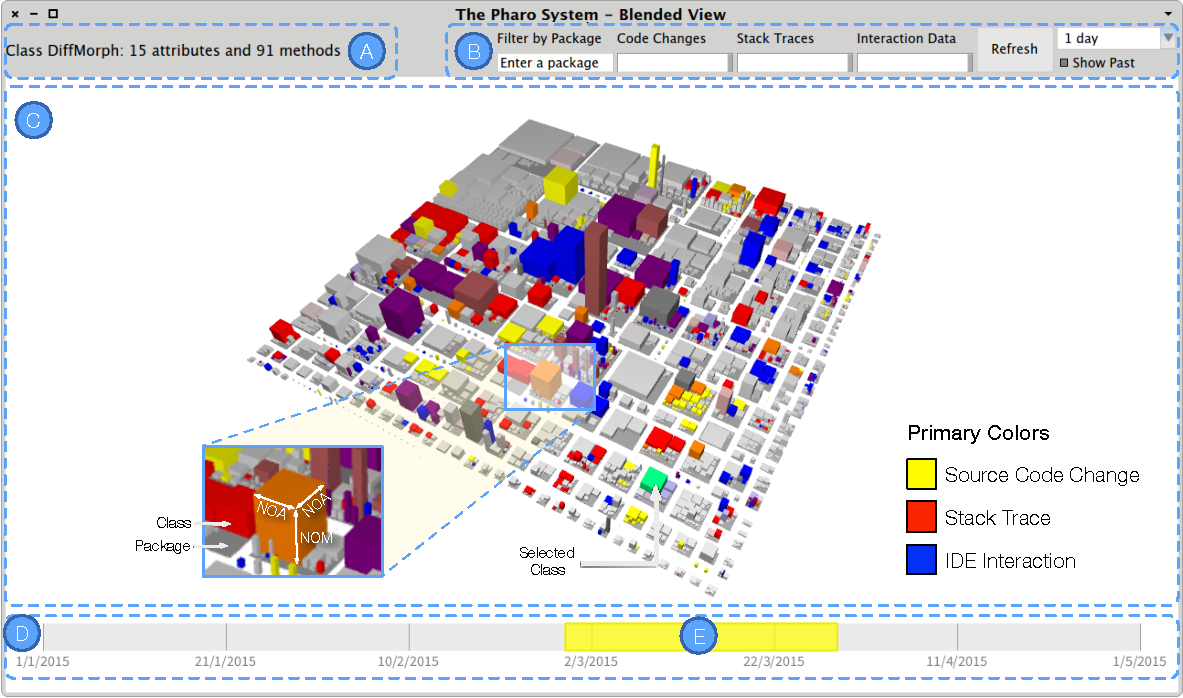
\includegraphics[width=.95\linewidth]{blend/visualization-principles}
\caption{The Blended City -- visualization principles and proportions}
\label{fig:visualization-principles}
\end{figure*}

\secref{sec:blend-ingredients} introduced the three ``ingredients'' of the visualization: source code changes, stack traces, and IDE interaction data.
Until now these diverse data sources are processed and visualized in isolation, leading to an incomplete view of the system.
Our goal is to visualize all these ingredient to enable a quick and comprehensive assessment of what happened to a software system in a given time frame.
To do so, we propose the \emph{``Blended City''}, a visualization that uses the \emph{City Metaphor} to depict all the ingredients of a software system.
Wettel and Lanza initially used this metaphor in \texttt{CodeCity}, a tool that depicts software systems as cities~\cite{Wett2007}.
In addition to the structural source code information presented by \texttt{CodeCity}, our Blended City uses a mixture of colors to depict different aspects of the software system itself.
\figref{fig:visualization-principles} shows an example of our visualization.

%%%%%%%%%%%%%%%%%%%%%%%%%%%%%%%%%%%%%%%%%%%%%%%%%%%%%
\subsection{In Practice}

\figref{fig:visualization-principles} shows the tool that we implemented to visualize the Blended City.
It is composed of four main parts: A status bar to display additional information on the selected entity (Fig.~\ref{fig:visualization-principles}.A), a toolbar to customize the visualization (Fig.~\ref{fig:visualization-principles}.B), the view canvas (Fig.~\ref{fig:visualization-principles}.C), and a timeline slider (Fig.~\ref{fig:visualization-principles}.D).
With the timeline slider the user chooses the visualized data timespan.
The width (\ie granularity) of this slider can be adapted using the dropdown menu on the right part of the toolbar.
In the example of \figref{fig:visualization-principles} the user selected one month of data, starting from March 1st.
 The toolbar (Fig.~\ref{fig:visualization-principles}.B) also features a text-input and a set of sliders.
The former enables simple queries to highlight particular packages in the system while the latter let the user choose the visual weight of each of the three ingredients of our visualization.
These weights affect the intensity of the color associated to each of the ingredients.
In the example of \figref{fig:visualization-principles}, all the sliders are at 100\%, thus all the ingredients have the same importance.
\figref{fig:stack-and-half-interaction}, instead, shows the data presented in \figref{fig:visualization-principles} giving high importance to stack traces (100\%), little importance on interaction data (50\%), and no importance to source code changes.

\begin{figure}[t]
\centering
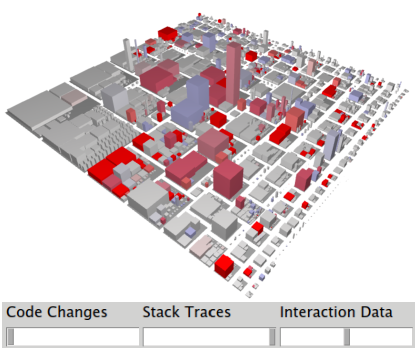
\includegraphics[width=0.65\linewidth]{blend/stack-and-half-interaction}
\caption[The view depicted in \figref{fig:visualization-principles}]{The same view depicted in \figref{fig:visualization-principles} with the following weights: 0\% source code changes, 100\% stack traces, and 50\% interaction data}
\label{fig:stack-and-half-interaction}
\end{figure}

In addition to changing the weights of the three components and the granularity of the visualized timespan, the view also features standard interactions such as panning and rotation in the 3D space.
Moreover, the user can click on an entity and get additional information on the status bar.
In \figref{fig:visualization-principles} the user selected the class \texttt{DiffMorph} and the tool shows that this class has 15 attributes and 91 methods (see \figref{fig:visualization-principles}.A).
Selected entities are colored with a bright green.


%%%%%%%%%%%%%%%%%%%%%%%%%%%%%%%%%%%%%%%%%%%%%%%%%%%%%
\subsection{The City Metaphor: Layout and Metrics}

In the city metaphor every  district of the city is a package and the buildings, contained inside the districts, represent the classes~\cite{Wett2007}.
The view uses a rectangle-packing algorithm to create the layout and it is \emph{polymetric}, \ie each dimension of the visual entity is proportional to a particular metric of the program entity being represented~\cite{Lanz2004}.
Since the visualization is 3D, classes are cuboids and have 3 dimensions that correspond to three metrics.
Our visualization, similar to the original \texttt{CodeCity}, uses the same metric for both width and depth and a different measure for the height.
In particular, we use number of attributes (\ie NOA) for both width and depth of a class and number of methods (\ie NOM) for the height of the cuboid representing a class.
The magnification in \figref{fig:visualization-principles} exemplifies these mappings.

%%%%%%%%%%%%%%%%%%%%%%%%%%%%%%%%%%%%%%%%%%%%%%%%%%%%%
\subsection{Color Harmonies and Blends}

Our Blended City presents different types of data, from structural properties of source code to stack traces and interaction data.
Structural source code relationships (\ie nesting of the package and software metrics) are the foundations for the layout while colors present the remaining information.

We use a triadic color scheme made of primary colors to present this information: Yellow for source code changes, red for stack traces, and blue for interaction data.
\figref{fig:color-wheel} shows a the color wheel with an emphasis on the triadic color scheme, where colors are evenly spaced around the color wheel.

\begin{figure}[ht]
\centering
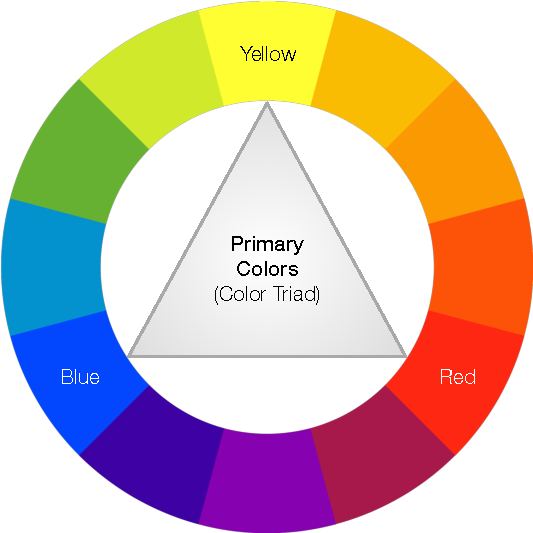
\includegraphics[width=0.4\linewidth]{blend/color-wheel}
\caption{Color wheel and triadic color scheme}
\label{fig:color-wheel}
\end{figure}

This offers strong visual contrast while retaining balance, and color richness.
Using colors equally spaced around the color wheel facilitate the addition of extra sources of information, \ie when we need to display \texttt{n} sources of information, we can create a new color harmony composed of \texttt{n} colors evenly spaced around the color wheel.


\subsubsection{Color Blends}

The three primary colors can only depict entities which are affected by a single of the three information sources.
However, in a given timespan a class might be affected by both IDE interactions and stack traces, for example when a developer is adding new functionalities to a class and testing them.
To depict this information, we use linear color blends between the different sources of information.
A class with both IDE interactions and stack traces is depicted in purple, the linear blend between the color of IDE interactions (\ie blue) and stack traces (\ie red).
\figref{fig:color-blends} shows examples of the different linear color blends on the triadic color scheme adopted by our visualization.
In this work we only considered the linear blending of colors.
It is part of our future work the investigation of different techniques to combine the colors, \ie color-weaving.

\begin{figure}[ht]
\centering
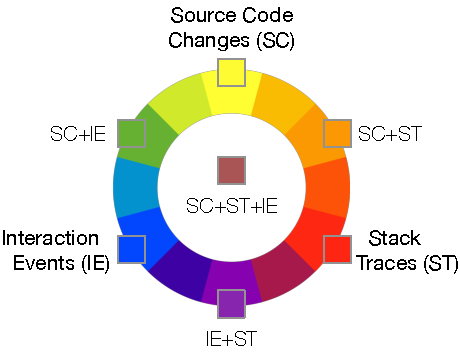
\includegraphics[width=.55\linewidth]{blend/color-blends}
\caption{Linear color blend on triadic color scheme}
\label{fig:color-blends}
\end{figure}


\subsubsection{Aging Mechanism}

When the user selects a timespan to visualize, the tool pre-loads and displays also the data happening in the immediately preceding interval (of the same length).
This enables the user to draw conclusions from the visualization having also in mind what happened immediately before.
To show this data, the tool uses an \emph{aging mechanism} that linearly reduces the color saturation as the age of the datapoint grows, \ie the older the more intense fading towards the default color of nodes (\ie gray).
\figref{fig:color-aging-timeline} shows how colors fade with such mechanism in a timeline.

\begin{figure}[!ht]
\centering
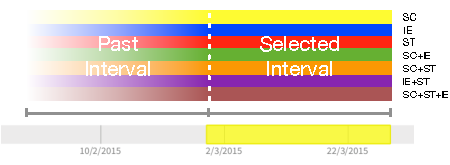
\includegraphics[width=0.8\linewidth]{blend/color-aging-timeline}
\caption{Aging process: example in the timeline}
\label{fig:color-aging-timeline}
\end{figure}

%\begin{figure}[ht]
%\centering
%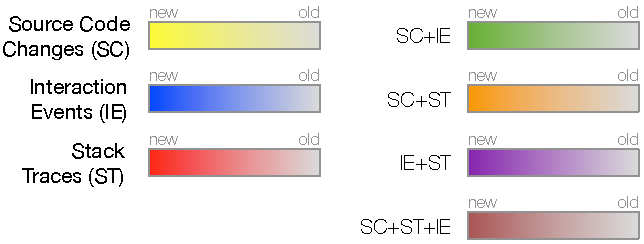
\includegraphics[width=\linewidth]{blend/color-aging}
%\caption{Aging Process: Plain and Blended Colors Fades Towards Gray}
%\label{fig:color-aging}
%\end{figure}

In the ``present'' interval (\ie the one selected by the user), colors are at their default saturation.
In the ``past''  interval, instead, the color saturation fades.
At the end of this interval, the nodes have the default color, \ie light gray.



\begin{figure*}[ht]
\centering
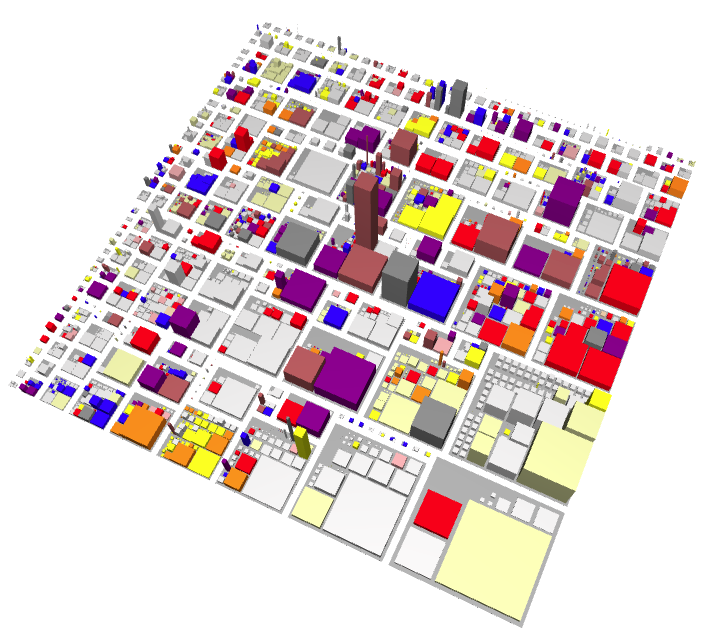
\includegraphics[width=.95\linewidth]{blend/full-view}
\caption{View of the city with all the activities}
\label{fig:full-view}
\end{figure*}



\subsection{Under the Hood}

The tool deals with a large volume of entries coming from heterogeneous data sources.
To conveniently manage them we standardized their format, using different data pre-processors, and store them in a central place.
We use \textit{MongoDB}\seeurl{http://mongodb.org/} databases to conveniently store the data.

When the user selects a timespan to visualize (Fig.~\ref{fig:archi}.1), the tool loads the data through optimized \textit{MongoDB} queries  (Fig.~\ref{fig:archi}.2) and builds the blended model of the data  (Fig.~\ref{fig:archi}.3).
Later it computes the city layout, applies the blended color scheme, and presents the view to the user (Fig.~\ref{fig:archi}.4).
The user can then use the toolbar to refine the visualization (Fig.~\ref{fig:archi}.5).

\begin{figure}[!ht]
\centering
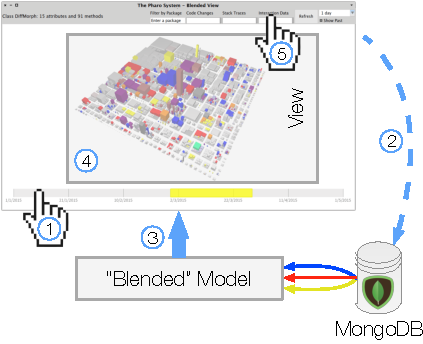
\includegraphics[width=0.75\linewidth]{blend/archi}
\caption{The architecture of the Blended City}
\label{fig:archi}
\end{figure}



\section{Telling Evolutionary Stories}\label{sec:blend-stories}

This section presents four stories, supported by our blended view, that narrate the evolution of the \pha system.


\subsection{Those Awkward Neighbors}

By selecting the full available timespan of the data we obtain a visualization that displays all the activities that involved the \pha system over a period of five months.
This enables to obtain a comprehensive view of the system evolution and derive long-term considerations and properties.
\figref{fig:full-view} shows the overall view of the available data.
One interesting example is represented by what we call the \emph{awkward neighbors}, \ie big but silent packages that have little or no activity.

In the lower part of \figref{fig:full-view}, we can spot two big packages that contain entities that are mostly colored with grey, meaning that they had almost no activity in the whole timeframe.
Moreover, they present almost no change in the entities they are composed of, and since the color of the changes is blended, those are all antecedent to the selected start date.
This means that in the last release they have been mostly ignored.
These two districts are the packages \textit{Graphics-Files} and \textit{Compiler}, whose details are shown in \figref{fig:packages-details}.

\begin{figure}[ht]
\centering
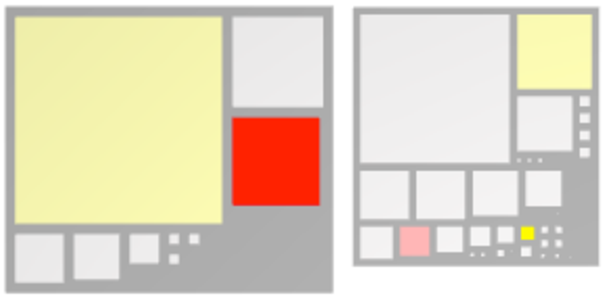
\includegraphics[width=0.5\linewidth]{blend/packages-details}
\caption{Details of the packages \textit{Graphics-Files} and \textit{Compiler}}
\label{fig:packages-details}
\end{figure}

A further investigation of the package \textit{Graphics-Files} reveals that it contains 10 classes.
These classes are dedicated to exporting graphics and writing them in different file formats.
Since \pha stores the dates of the changes of a method, we can determine when the changes took place.
We can see that there are three main batches of changes: A small update in 2014, regarding a small refactoring of an error message, one in 2001 and one in 1997.
This is interesting, because it indicates that the package has been part of the system for a long time, it had little changes and is by now a solid foundation of the system.
Similarly, the package \textit{Compiler} contains 46 classes, and apart from some recent modification in 2013 to the structure of the compiler, many of the methods are unmodified since 2006, 2003, or 1998.

One might wonder how it is possible that some parts are older than the \pha project itself.
The reason is that \pha was born as a fork of the \textsc{Squeak} project\seeurl{http://www.squeak.org}, which in turn is a re-implementation of the original \textsc{Smalltalk-80} system, which was evolved from the \textsc{Smalltalk-72} system.
This means that some of the methods and classes in these packages might very well be 40+ years old.

%%%%%%%%%%%%%%%%%%%%%%%%%%%%%%%%%%%%%%%%%%%%%%%%%%%%%%%%%%%%
\subsection{Market Districts}

While examining some of the packages with the most activities, we found districts with many interactions from all three data sources, and we call them \emph{market districts}.
\figref{fig:market-districts} shows an example of market districts corresponding to the packages of \textit{Spec} and \textit{Morphic}.
Morphic is the core graphic library of \pha, while Spec is a framework to build user interfaces, built on top of Morphic.

\begin{figure}[ht]
\centering
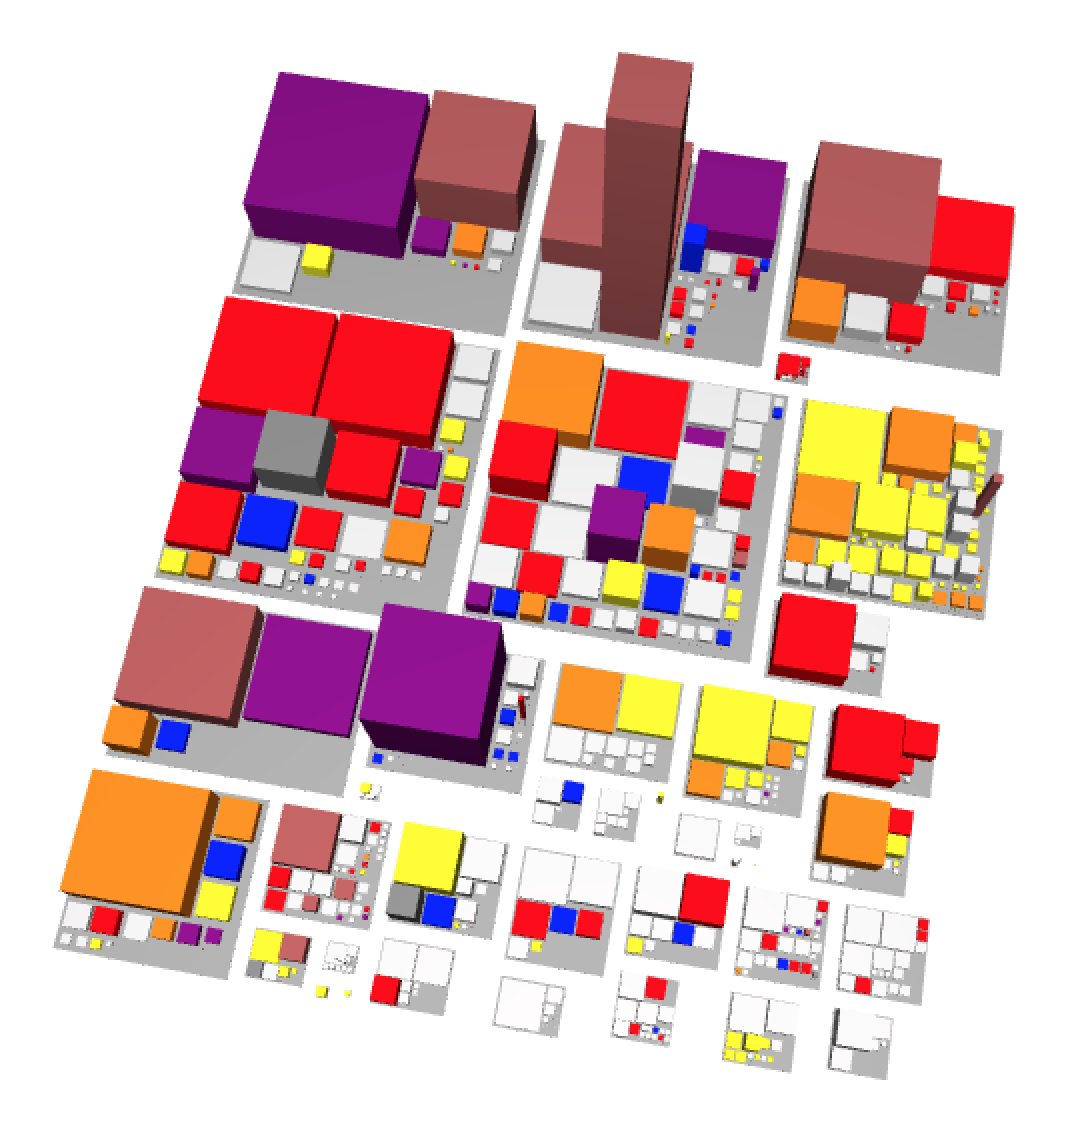
\includegraphics[width=.7\linewidth]{blend/red-district-packages}
\caption{\textit{Spec} and \textit{Morphic} market districts}
\label{fig:market-districts}
\end{figure}

Many classes are involved in exceptions, they were recently changed or they were subject to developer interactions.
This reveals a long known problem in the community, that is, the fact that the code of Morphic is old and has been ported through various platforms.
 The case of Spec is similar: since Spec is a framework built on top of Morphic, it shares its weakness and part of its complexities.

Differently from the awkward neighbors (shown in \figref{fig:packages-details}), the market districts for Morphic and Spec are not settled and solid: Instead, they are often causes of bugs and issues.
The view also shows that many classes that act as entry points received frequent developer interactions, meaning that they likely have an unclear public interface.

Moreover, we can see that the Morphic packages are still frequently changed, showing that the community is constantly trying to fix the codebase.
Finally, the high number of classes involved in the stack traces suggests that the code modification, together with the difficulty of understanding the API, is likely a cause of many programming errors.
In particular, there are some \emph{hotspots}, \ie packages where classes are mostly colored in red only.
These classes are involved in failures, but they are rarely modified or involved in interaction data.

These theses are confirmed by the fact that the community is trying to replace the code of Morphic with a new, polished and easy-to-use replacement called \textit{Bloc}, to address issues that we can be spot in \figref{fig:market-districts}.
However, as the complexity of the picture suggests, replacing this code is not an easy task, and has been work-in-progress for more than a year now.


%%%%%%%%%%%%%%%%%%%%%%%%%%%%%%%%%%%%%%%%%%%%%%%%%%%%%%%%%%%%

\begin{figure*}[ht]
\centering
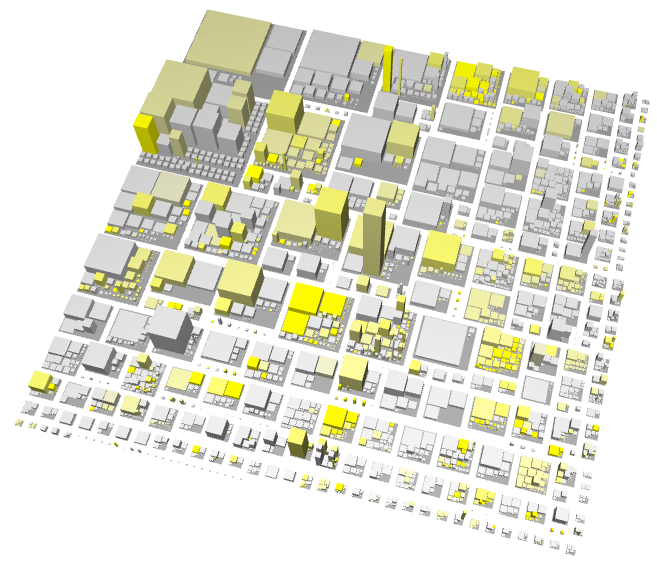
\includegraphics[width=0.75\linewidth]{blend/pharo-changes}
\caption{Changes in the \pha system}
\label{fig:pharo-changes}
\end{figure*}

\subsection{New in Town}

During the development of \pha 4, many classes got updated and some new components were added.
We want to analyze the progressive introduction of these changes, and how they impacted the system after the integration.
We then use the sliders in Fig.~\ref{fig:visualization-principles}.B to remove all the data sources, except for the changes.
\figref{fig:pharo-changes} shows in full yellow the entities touched by a change in the last five months, and in blended yellow the changes in the previous five months.
We can verify that there are elements that remained untouched, while some others were subject to intense development.

By moving the slider we can select a timespan to restrict the changes to a given moment of the story of the components and inspect the status of the system during time.
We can notice that from a certain point on there was the appearance of packages related to the \emph{GT-Tools}, a set of tools to improve the interaction with the objects in the system.
By restricting the timespan to the beginning of January (\ie the first appearance of activities), to determine the moment of integration.

\begin{figure}[h]
\centering
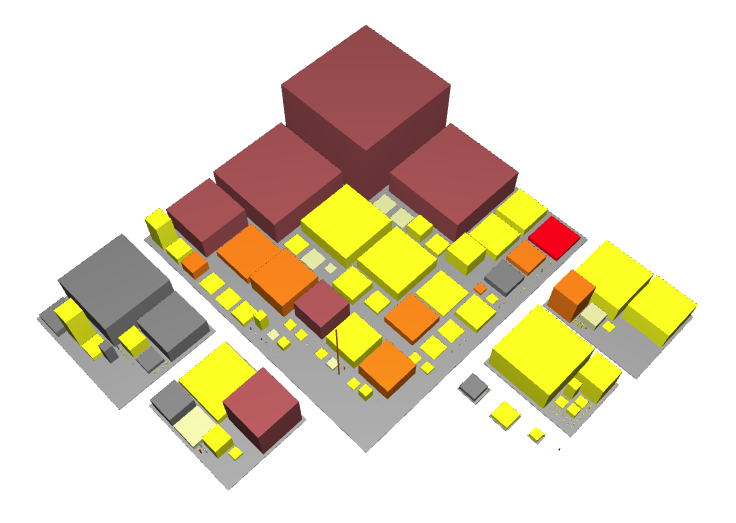
\includegraphics[width=.8\linewidth]{blend/gt-packages}
\caption{The changes of \textit{GT-Tools} packages}
\label{fig:gt-spotter-packages}
\end{figure}

\figref{fig:gt-spotter-packages} visualizes the blended city for the \emph{GT-Tools} packages.
Some classes are involved in all three data sources, \ie they are colored in dark brown.
This can be explained by the fact that the first phases of integration usually require adaptation, refinement, and debugging, thus generating (other than changes) frequent exceptions and developer interactions.

The other interesting observation that we can derive from the visualization is that the  classes involved in user activities are also the biggest.
This can be explained by considering that those classes act as main entry points to the package, a starting point for developers who want to use or inspect the code.

%%%%%%%%%%%%%%%%%%%%%%%%%%%%%%%%%%%%%%%%%%%%%%%%%%%%%%%%%%%%

\begin{figure*}[ht]
\centering
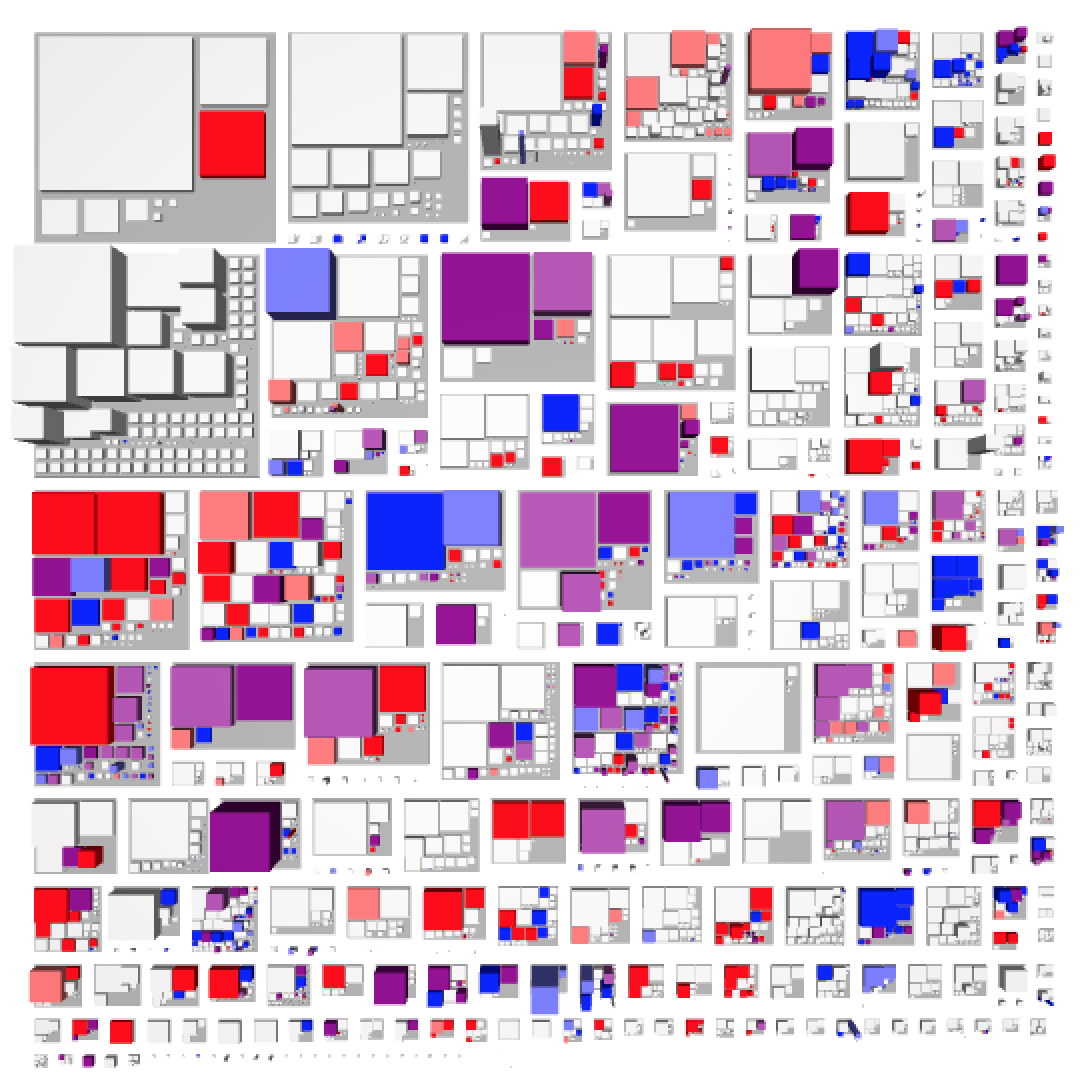
\includegraphics[width=0.9\linewidth]{blend/traces-and-interactions}
\caption{A view of the system highlighting stack traces and developer interactions only}
\label{fig:traces-and-interactions}
\end{figure*}

\subsection{The Purple Buildings}

A benefit of our blended city approach is that a data source can be removed to spot behaviors that are independent from it.
\figref{fig:traces-and-interactions} shows the blended city for \pha with only stack traces and developer interactions.
While the stories we presented so far try to consider the code entities at a package level,  the blended city without changes reveals the interesting role of some classes.

 Scattered across the system, there are some big and medium classes colored of purple without apparent correlation with the color of its neighbors.
By inspecting their names, we find examples like \textit{DateAndTime}, \textit{Float}, \textit{Job}, \textit{SmalltalkImage}, \textit{Socket}, \textit{SocketStream},  \textit{SystemWindow}, \textit{TestRunner}, and many others related to rendering of graphics, that we covered in the previous stories.
These classes are not problematic \emph{per se}, but represent an interesting area of the system that we could define as \emph{Advanced APIs}.
These classes appear in many stack traces and in many development interactions, an information that suggests that they occour near the source of the exceptions, when these exceptions are not directly generated from them.
This context could signify that the user is trying to understand a class that has a name suggesting a behavior, but that she needs some further understanding to learn how to use the objects of the class by trying the various methods.

The use of this information could be used by the maintainer of the system to prioritize the areas of that could need more public documentation, to ease the learning process of those entities and their API.

Note that the same information, blended with the addition of code changes and applied to classes that are not part of the core system, could signify that a developer is applying a \textit{Test Driven Development} approach, by implementing incomplete methods and completing them whenever the system tries to execute a method that is not yet implemented, a common practice in the Smalltalk community~\cite{black2009}.


\section{Discussion}\label{sec:blend-discussion}

Developing our approach we became aware of many details that are hard to grasp in terms of how the users interact with the code entities.
We believe that an important next step for this analysis would be to improve the system by providing updated information on fresh data mined in real-time.

Our visualization considers activity data, but maps this information on the static entities of the system.
However, in Object Oriented Programming, the main focus lays on how these entities communicate among them, rather that how these objects are structured internally.
We think that this approach could be further improved by also considering the interactions caused by the messages sent as a result of the interactions.
%We want to deepen this perspective, and produce more refined views that could represent the true dynamic nature of a software and present a system as a network of messages correlated with the user interactions.

Finally, from the user stories we saw how to retrieve information about the evolution of the system by looking at the way users interact with it.
We think that a similar approach of combining data can be effectively put into use when analyzing old code, to understand and maintain legacy systems and support software archaeology.



\section{Outline}\label{sec:blend-summary}

Software visualization and analysis usually focus on giving a detailed representation of a single aspect of the examined entities.
We presented an approach where we visualize data from three different data sources and contexts, blending them to produce multi-dimensional information about a system, its code and how developers interact with it.
We considered a combination of system changes during the development phase of a system, the interaction data generated by users and the stack traces of the exceptions triggered during the daily usage of the platform.

We presented a tool that visualizes our blended information on a city view of \pha, a dynamic, flexible and active programming ecosystem.
We showed how our tool allows to select different timespans and weigh the diverse components, to enable a fine grained inspection of each entity during its recent evolution.
We think that our approach has a real potential to be successfully applied in a development context to allow for multi-dimensional incremental and interactive analysis of a system, supporting a deeper understanding of the code entities by highlighting the synergies among its recorded activities, and the relations and interesting behaviors otherwise hidden or harder to detect.
We illustrated four stories where we extract and analyze some real-world issues by looking at the blending of the data and identifying some existing problems, or finding suggestions for problems that could be addressed by the maintainers of the platform to improve the system.
We believe that the knowledge highlighted by our approach can help in presenting and tackling existing problems and provide a deeper understanding of a system.

In the last chapters we saw how we can collect information about the errors on a system and exploit this data to support debugging, understand how a system is used, and navigate its evolution.
In this chapter we presented a use case were we combined the data we collected together with additional data sources, to create a wide-ranging representation of the history of a system.
By using our tool, a developer can improve her comprehension of a system and understand how a system is used by its users.
We saw that we can collect and store data in an effective way and with a powerful representation.
However, being able to collect any kind of data does not tell us \emph{what} we should collect.
In other words, we still have to understand \emph{how} to improve the representation of a bug report.
In the next chapter we investigate the data contained in several in issue tracking systems, and how it impacts the resolution of a defect.
By looking at this data, we try to distill the model for a minimal bug report.


\part{Modeling}
  %!TEX root = ../tommaso-thesis.tex
%!TEX spellcheck = en_US


%-------------------------------------------------------------------------------------------
% Research Questions and Results
%
\newcounter{RQCounter}
\newcounter{RQACounter}

%Pass in label for rq, then rq
%

\newcommand{\RQ}[2]{%
\refstepcounter{RQCounter} \label{#1}
 \begin{framed}
  % \begin{examplebox}
   \textbf{RQ\arabic{RQCounter}.}~#2
  % \end{examplebox}
\end{framed}
}


% \chapter{What Makes a Satisficing Bug Report?}\label{ch:model}
\coolchapter{What Makes a Satisficing Bug Report?}{}{ch:model}


To ensure quality of software systems, developers use bug reports to track defects.
It is in the interest of users and developers that bug reports provide the necessary information to ease the fixing process.
Past research found that users do not provide the information that developers deem \emph{ideally useful} to fix a bug.
This raises an interesting question: What is the \emph{satisficing}\footnote{Satisficing is a neologism coined by Simon~\cite{Simo57,Simo01} combining the verbs {\em to satisfy} and {\em to suffice}, and it is used to describe a solution that is roughly satisfactory and meets some criteria of sufficiency and is better than an optimal solution that would be too complex or would imply too strong constraints.} information to speed up the bug fixing process?

We conducted an observational study on the relation between provided report information and its lifetime, considering more than 650,000 reports from open-source systems using popular bug trackers.
We distilled a meta-model for a \emph{minimal} bug report, establishing a basic layer of core features.
We found that few fields influence the resolution time and that customized fields have little impact on it.
We performed a survey to investigate what users deem easy to provide in a bug report.

\structure
In \secref{sec:model-intro} we discuss what we should expect from a bug report.
\secref{sec:model-method} presents our research method and introduces our research questions, that we answer in \secref{sec:model-approach}.
In \secref{sec:model-discussion} we discuss the meaning of our findings and how our work can be extended, while in \secref{sec:model-summary} we summarize and conclude the chapter.

\newpage


%%%%%%%%%%%%%%%%%%%%%%
\section{Good Bug Reports vs. Real Bug Reports}\label{sec:model-intro}
%%%%%%%%%%%%%%%%%%%%%%

When users file a bug report for a software project, their main hope is that developers will fix it quickly, to minimize its impact.
But what information should they provide to make this happen? There is a stark mismatch between what developers perceive as \emph{optimally} useful in this respect (\ie steps to reproduce, stack traces, and test cases) and what users are effectively able, or sometimes just willing to provide, when filing a bug report~\cite{Zimm2010a}.

Bug tracking systems and software projects should define a reasonable common ground for information to be provided in bug reports, so that it is not too demanding for users, yet provides enough information to developers.
Nevertheless, considering what popular issue trackers and projects (\eg \emph{Bugzilla}, \emph{JIRA}, \emph{FogBugz}, and the issue tracker provided with \emph{GitHub}) demand from users, we see that it is quite diverse and specialized.
In particular, each bug tracking system provides a core set of common fields, which are often complemented with additional fields.
Such  fields may reflect requirements for specific domains, or represent additional data customizable by project owners.

For example, the commercial issue tracker JIRA defines several fields that describe in detail aspects pertaining to the time management of issues, while the GitHub issue tracker provides a minimal (and sometimes criticized\footnote{\url{https://github.com/dear-github/dear-github}}) model that, together with the integration with the Git versioning system, conceives a bug report as a conversation among developers, fostering the philosophy of collaborative development proposed by GitHub~\cite{Thun2013}.

Overall, there is currently no consensus among software projects and creators of bug reporting systems on essential mandatory fields to be filled by users in each report, optional fields that give useful additional information, and free space for users willing to provide more detailed descriptions.

Our vision is to define the minimum set of information needed to describe a software defect, to clarify what should be required by each bug reporting system.
In this chapter, we make a step in this direction: We investigate what makes a \emph{satisficing} bug report.
We move from defining a good or more precisely an \emph{optimal} bug report and adopt a more pragmatic view on what users should provide.

%This goal requires to consider the amount of required information, the reliability of the data, and the evolution of the report during its lifetime.

We conduct our investigation in three steps: \begin{inparaenum}[(1)]
\item We investigate what users and developers perceive as \emph{difficult} in writing a report, by means of an online questionnaire;
\item we investigate the usage and evolution of issue tracker data, by means of a large-scale quantitative analysis of the status changes in submitted bug reports and the impact that customized fields have on the resolution of a defect;
\item we study which fields developers use to describe defects, by means of a further quantitative analysis on the lifetime of reports in relation to the evolution of report's state and its \emph{completeness} in its core and customized fields.
\end{inparaenum}

Our results show that providing more fields in a report relates to the fixing time: In particular, the bug reports with longer descriptions tend to be solved quicker.
While this might be intuitive, issue trackers still do not emphasize this aspect during the submission of a new bug report, putting the accent on the customization capabilities of the platform.
At the same time, the project-specific bug report fields have little impact to the fixing time.
This chapter provides insights on the current issue tracking practices and defines guidelines in building the foundations for a new model of an issue tracking system.

\newpage
The contributions presented in this chapter are:

\begin{itemize}[$\circ$]

\item A survey that identifies the components of a bug report considered difficult to provide by users (\secref{sec:model-survey}).

\item A dataset of 650,000 bug reports, collected from the issue trackers of \bzilla and \jira (\secref{sec:model-collection}).

\item The model for a minimal bug report, that puts the emphasis on the shared components of a bug report (\secref{sec:model-model})

\item An analysis of the usage of the fields in an issue tracker, from active open source projects (\secref{sec:model-fields}).

\end{itemize}




% %%%%%%%%%%%%%%%%%%%%%%%%%%%%%%%%%%%
% \section{Issue Tracking Systems}\label{sec:model-bugtrackers}
% %%%%%%%%%%%%%%%%%%%%%%%%%%%%%%%%%%%
%
% To obtain an overview of the salient features of issue trackers, we briefly present four platforms, selected by importance and overall adoption in open-source systems: \bzilla, \jira, the \gth issue tracker and \fbz.
%
% \subsubsection{Bugzilla} One of the oldest and most popular issue tracking systems that influenced many other issue trackers.
% Developed by the Mozilla Foundation, it is used both by open source projects\seeurl{https://www.bugzilla.org/installation-list/} (\eg Linux) and by industrial and government customers (\eg NASA).
% The Mozilla Foundation itself uses \bzilla to manage the issues of its projects, like Firefox.
% \bzilla includes several fields, allowing for a great level of detail in specifying an issue.
% However, such a freedom of choice also produces a complex interface where many of the values are often left empty, or set to their default value.
% \figref{fig:bugzilla-interface} shows a typical submission form with both fields for fixed-option choices and text boxes for narrative (\eg to describe how to reproduce the bug).
%
% \begin{figure}[ht]
% \centering
%   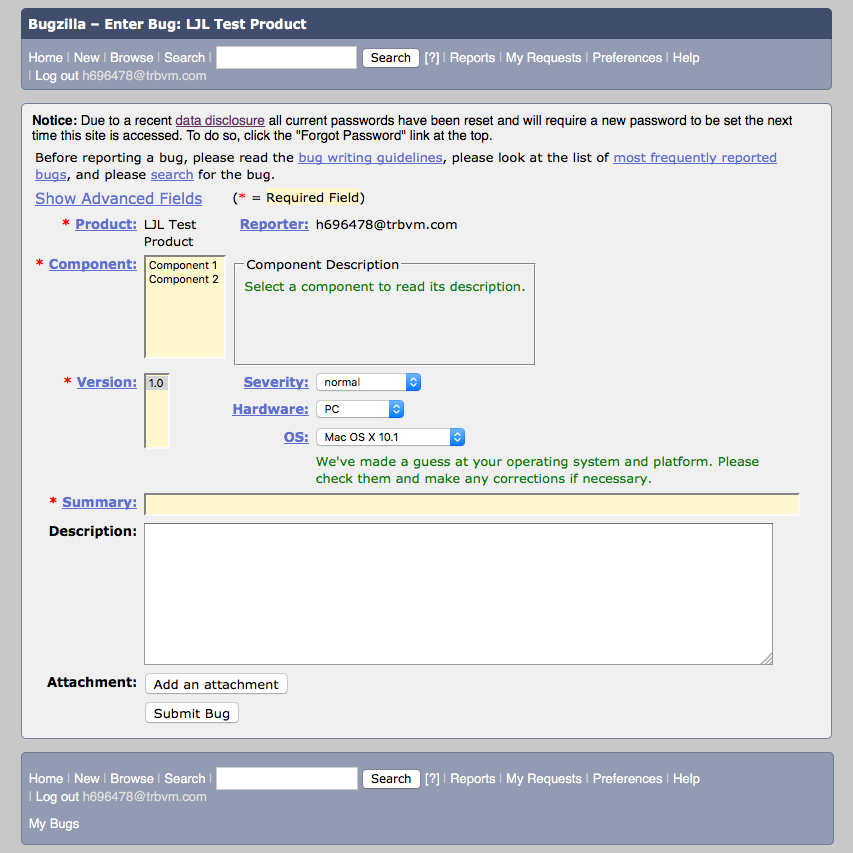
\includegraphics[width=.9\linewidth]{model/bugzilla}
%   \caption{Bugzilla Submission Form}
%   \label{fig:bugzilla-interface}
% \end{figure}
%
% \subsubsection{JIRA} A successful commercial bug reporting systems used by several customers like Twitter, Linkedin, and Ebay.\seeurl{https://www.atlassian.com/company/customers} \jira supports the same model as \bzilla, augmenting its capabilities with a polished user interface and a tight integration with other development tools, especially with the version control system.
%
%
% \subsubsection{GitHub} A popular web-based \textsc{Git} repository hosting service, used for the development of several popular open source projects.
% Together with the \textsc{Git} hosting service, \gth offers a simple issue tracker to manage the defects during development.
% \figref{fig:github-interface} shows the interface of the \gth bug submission form.
%
% \begin{figure}[ht]
% \centering
%   \includegraphics[width=\linewidth]{model/github}
%   \caption{GitHub Bug Submission Form}
%   \label{fig:github-interface}
% \end{figure}%
%
% \gth adopts a simplified model of a bug report and a strong integration with the source code (thus giving the possibility to link issues with specific commits).
%
% \subsubsection{FogBugz} In this system, the model of a bug report is similar to \bzilla, but more polished and user-friendly, due to its clean user interface and filtering capabilities.
% Differently from \gth, \fbz\seeurl{https://www.fogcreek.com/fogbugz/} does not simplify the report model, but it lets users add custom filters and views.

\subsubsection{Reflection} To understand the essential traits of bug reports, we analyze how the data included in bug reports influences their lifetime.
We next analyze the features of a set of bug reporting systems, to distill a model of common/specific fields for their bug reports.
This model serves as a basis for further empirical analysis, to determine how these commonalities and customizations influence the life of the reports.


%%%%%%%%%%%%%%%%%%%%%%%%%
\section{Research Method}\label{sec:model-method}
%%%%%%%%%%%%%%%%%%%%%%%%%

To determine what makes a satisficing bug report, we first need a way to rate the quality of a bug report, then we can conduct quantitative analysis to determine which features relate with higher quality.
Measuring the quality of bug reports is hard to do in an automated and unbiased way.
For this reason, researchers proposed different metrics to measure it~\cite{Hooi2007}, all with their limitations, but reasonable enough to be realistic.
In this work, we decide to consider the \emph{lifetime} of a bug report (\ie the time between the opening and resolution of a defect) as a viable proxy for its quality rating, as the time spent dealing fixing software defects is crucial in reducing the time the system contains a problem.
Limitations of this proxy metric include the fact that the trivial bugs, or the non-issues, are the ones that require less time to fix, and that the severity can also have a not negligible impact on how quickly developers decide to fix a problem.
Nevertheless, the information shared in the bug report has to be satisficing enough to let developers understand whether it is a trivial fix, an urgent matter, or something that can wait longer.
For this reason, we find lifetime of a bug report a useful approximation in aggregate statistical analyses to provide a high-level view over bug repositories.

We investigate how users and developers use issue tracking systems and the impact that the provided information has on the lifetime of a bug report.
According to Zimmermann \etal the information provided by submitter can be partial or incorrect~\cite{Zimm2010a}.
To understand what is reasonable for a user to provide in a report, we conducted a survey asking developers what they think are the difficult elements to provide.
We then focus on two of the main components that compose a bug report: (1) its state and (2) the core and optional attributes, to understand how the provided data is used.

%%%%%%%%%%%%%%%%%%%%%%%%%%%%%%%
\subsection{Research Questions}\label{sec:model-questions}

When collecting information about software defects, it is important to know when the submitted data is reliable and accurate.
Our goal is to investigate what  users can easily provide and what is harder to obtain; we structure our investigation into the following question:

\RQ{rq1}{What are the elements that are perceived as difficult to provide when reporting a defect?}

To understand the relationship between what is described in a bug report and its lifetime, we have to consider the different kind of data that reports can provide.
This is not trivial, because different platforms offer different fields to provide information, with different meaning and values.
As a first step for our quantitative evaluation, we investigate how to define a meta-model to comprehensively describe information stored across different issue reporting systems:

\RQ{rq2}{What is a comprehensive unified meta-model for describing data from different bug tracking systems?}

After having defined the meta-model, we can quantitatively investigate several aspects of reports related to their lifetime and evolution.
During development, a bug report changes its state, sometimes several times, ideally converging to a closed state.
The changes in the state of a report are important to understand its evolution~\cite{DAmb2007b}.
We are interested in considering the evolution of the states and see whether the aggregate of these changes can provide knowledge on the inner logic of an issue tracker.
This leads to the following question:

\RQ{rq3}{What are the most frequent states and state transitions in bug reports?}

Together with a state, a bug report comes with a set of attributes that describe the properties of a report.
These attributes can also be defined by the users, to create project-specific customized fields.
We investigate the completeness of core and custom fields with respect to the lifetime of a bug, considering the following research question:

\RQ{rq4}{Does the completeness of standard and project-specific attributes in a bug report relate to its lifetime?}

To answer our questions, we both run a survey (\secref{sec:model-survey}) and we collect, model, and analyze a large dataset of bug reports from open source projects (\secref{sec:model-collection}).

%%%%%%%%%%%%%%%%%%%%%%%%%%%%%%%%%%%%
\subsection{Online Questionnaire} \label{sec:model-survey}

Zimmerman \etal asked users and developers what they think are the useful elements in a bug report and how hard it is, in their opinion, to provide those elements~\cite{Zimm2010a}.
We proposed a similar questionnaire to the \emph{Pharo} open source community to further understand what it is reasonable to expect from users submitting a bug report.
The questionnaire is composed of two parts: \begin{inparaenum}[(1)]
\item We collect demographic information inquiring about expertise with programming and with submitting, handling, and fixing bug reports; and
\item we collect information about respondents' perception of how difficult it is to provide different kinds of information when submitting a bug report.
\end{inparaenum}
All the questions are formulated as statements (\eg ``It is easy to provide a description of the failure'') and the respondents have to declare their agreement using a 5-level Likert-type scale.
We map the results into an integer scale from $-2$ (\ie ``strongly disagree'') to $2$ (\ie ``strongly agree'').

\begin{table}[t]\small
\centering
\caption{Expertise of the participants of the survey (average)}\label{tab:survey}
\rowcolors{1}{tablefirstrow}{tablesecondrow}
\begin{tabular}{lr}
\rowcolor{tableheader} \textbf{Activity} & \textbf{Average} \\
\hline
Experience with Object Oriented programming languages & $1.5$ \\
Knowledge of Pharo & $1.3$ \\ \hline
Have often bug reports assigned & $-0.4$ \\
Often handle bug reports & $0.6$ \\
Often participate in discussion in bug reports & $0.3$ \\
Often submit bug reports & $0.7$ \\
\hline
\end{tabular}
\label{tab:survey-expertise}
\end{table}

We advertised the survey through the development mailing list of Pharo and we received a total of 22 complete responses.
\tabref{tab:survey-expertise} summarizes the respondents' expertise.
The respondents are experienced with object-oriented programming and with the Pharo IDE.
While they have experience in submitting and handling bug reports, their experience is lower in participating in discussions about bug reports and much lower in having reports assigned to them.
For this reason, we deem the respondents' sample to be in line with the aim of our survey.
In fact, we are especially interested in knowing the point of view of submitters of bug reports, rather than the view of the developers that ``consume'' these reports.


%%%%%%%%%%%%%%%%%%%%%%%%%%%%

\begin{table}[t]\small
\centering
\caption{Overview of the projects in the dataset}\label{tab:dataset-projects}
% \rowcolors{1}{tablefirstrow}{tablesecondrow}
\begin{tabular}{l|l|rrrrr}
 \rowcolor{tableheader}
 &               & \multicolumn{5}{c}{{\bfseries Issues}} \\
%Ecosystem
 \rowcolor{tableheader}
 & Project & First & Last & Count & Age (days) & Frequency \\
\hline
\multirow{9}{*}{\rotatebox[origin=c]{90}{Apache}}
 & Cassandra & Mar 7, 2009 & Jul 8, 2015 & 9,723 & 2,314 & 5h 42m \\
 & Hadoop & Jul 24, 2005 & Jul 8, 2015 & 10,191 & 3,635 & 8h 33m \\
 & Lucene & Oct 9, 2001 & Jul 8, 2015 & 6,641 & 5,019 & 18h 8m \\
 & Maven & Nov 20, 2002 & Jul 23, 2015 & 4,663 & 4,628 & 23h 49m \\
 & Mahout & Jan 30, 2008 & Jun 25, 2015 & 1,752 & 2,702 & 37h 6m \\
 & Pig & Nov 2, 2007 & Jul 7, 2015 & 767 & 2,804 & 87h 44m \\
 & Sorl & Jan 25, 2006 & Jul 8, 2015 & 7,728 & 3,451 & 10h 43m \\
 & Zookeeper & Jun 6, 2008 & Jul 3, 2015 & 2,207 & 2,582 & 28h 4m \\
\hline
\multirow{6}{*}{\rotatebox[origin=c]{90}{Mozilla}}
 & Air Mozilla & Apr 14, 2009 & Jun 16, 2015 & 509 & 2,254 & 106h 16m \\
 & Bugzilla & Apr 15, 1998 & Jul 27, 2015 & 19,395 & 6,312 & 7h48m \\
 & Core & Mar 28, 1997 & Jul 17, 2015 & 292,358 & 6,684 & 33m \\
 & Firefox & Jul 30, 1999 & Jul 8, 2015 & 155,078 & 5,821 & 54m \\
 & Firefox for Android & Sep 11, 2008 & Jul 28, 2015 & 18,906 & 2,510 & 19m \\
 & SeaMonkey & Nov 10, 1995 & Jul 27, 2015 & 92,757 & 7,198 & 1h 51m \\
 & Thunderbird & Jan 2, 2000 & Jul 8, 2015 & 42,247 & 5,666 & 3h13m\\\hline
\end{tabular}
\end{table}

\subsection{Data Collection} \label{sec:model-collection}

To understand what users and developers collect and provide in bug reports, we mined the contents of the issue trackers of several software projects.
To collect real development data for our study, we consider the Apache Foundation and the Mozilla Foundation: Both platforms contain a considerable number of popular and active open source projects, with years of development history.
Moreover, both platforms host several projects tracked on public, dedicated bug trackers: Mozilla uses \bzilla, Apache uses \jira.
They offer a public \textsc{REST} API to access their repositories in \textsc{JSON} format, allowing for a clean and reliable data collection.

We built a downloader and an importer to collect the data, serialize the contents of each report, and store the polished data in a \textsc{PostgreSQL} database.
\tabref{tab:dataset-projects} describes our dataset.

The dataset contains more than 650,000 bug reports, $15\%$ of which were still open during the data collection phase.
\tabref{tab:dataset} shows an aggregated summary of the dataset we collected.
Each bug tracker has a different set of bug report states.

\begin{table}[h]\small
\centering
\caption{Contents of the dataset}
\rowcolors{1}{tablefirstrow}{tablesecondrow}
\begin{tabular}{l|rrr}
 \rowcolor{tableheader}
 & Apache & Mozilla & Total \\
\hline
%Projects & 8 & 7 & 15 \\
Open issues & 7,545 & 91,336 & 98,881 \\
Closed issues & 36,127 & 529,914 & 566,041 \\
Total Issues & 43,672 & 621,250 & {\bfseries 664,922} \\ \hline
\end{tabular}
\label{tab:dataset}
\end{table}

\tabref{tab:dataset-statuses} details them, for each tracker, with the counts of the bug reports for each state at the moment of the download.

\begin{table}[ht]\small
\centering
\caption{Different states of bug reports in \bzilla and \jira, with the count of the reports currently in each state and the total sum of all the times a bug report reached a state.}
\rowcolors{1}{tablefirstrow}{tablesecondrow}
\begin{tabular}{l|l|rr}
\rowcolor{tableheader}{\bfseries Tracker} & {\bfseries State} & {\bfseries Current} & {\bfseries Total} \\ \hline
JIRA & Closed & 21,847 & 22,460 \\
& Resolved & 14,280 & 33,386  \\
&  Open & 6,736 & 43,203 \\
&  Patch Available & 471 & 18,944 \\
&  Reopened & 235 & 3,042 \\
&  In Progress & 84 & 2,175 \\
&  Awaiting Feedback & 14 & 15 \\
&  Testing & 4 & 86 \\
&  Ready to Commit & 1 & 3 \\ \hline
Bugzilla & RESOLVED & 391,919 & 579,488 \\
&  VERIFIED & 136,783 & 143,082\\
&  NEW & 65,816 & 353,264\\
&  UNCONFIRMED & 19,821 & 297,319 \\
&  ASSIGNED & 3,701 & 129,057 \\
&  REOPENED & 1,998 & 32,745 \\
&  CLOSED & 1,212 & 1,537 \\ \hline
\end{tabular}
\label{tab:dataset-statuses}
\end{table}

\subsection{Data Analysis Techniques}

The large volume of data we collected allows us to explore the usage of issue trackers and to investigate the common practices of bug tracking.
Understanding these aspects can help us to answer our questions and verify whether the usage of the properties of a tracker influences the life of a  report.

To investigate our research questions, we adopt the following approach.
To answer RQ3, we build a transition diagram of all the state changes for each issue tracker, to highlight the common patterns in the growth of a report, and we weight the diagram with the values from the dataset.
To answer RQ4, we build a machine-learning-based prediction model to verify how completeness of fields of a bug report relates to its lifetime.


%%%%%%%%%%%%%%%%%
\section{Results}\label{sec:model-approach}
%%%%%%%%%%%%%%%%%

The data we collected allowed us to reply to the research questions in \secref{sec:model-questions}.
We review them in order.

%%%%%%%%%%%%%%%%%%%%%%%%%%%%%%%%%%%%%%%%%%%%%%%%%%%%%%%%%%%%%%%%%%%%%%%%%%%%%%%%%%%%%%
\subsection*{RQ1: What are the elements that are perceived as difficult to provide while reporting a defect?}

We asked respondents how easy it is to provide 13 different elements in a report, using a 5-level Likert scale from $-2$ (``strongly disagree'') to $2$ (``strongly agree'').
\figref{fig:survey} shows a summary of their answers, sorted by increasing difficulty as reported by the respondents.
%
\begin{figure}[t]
\centering
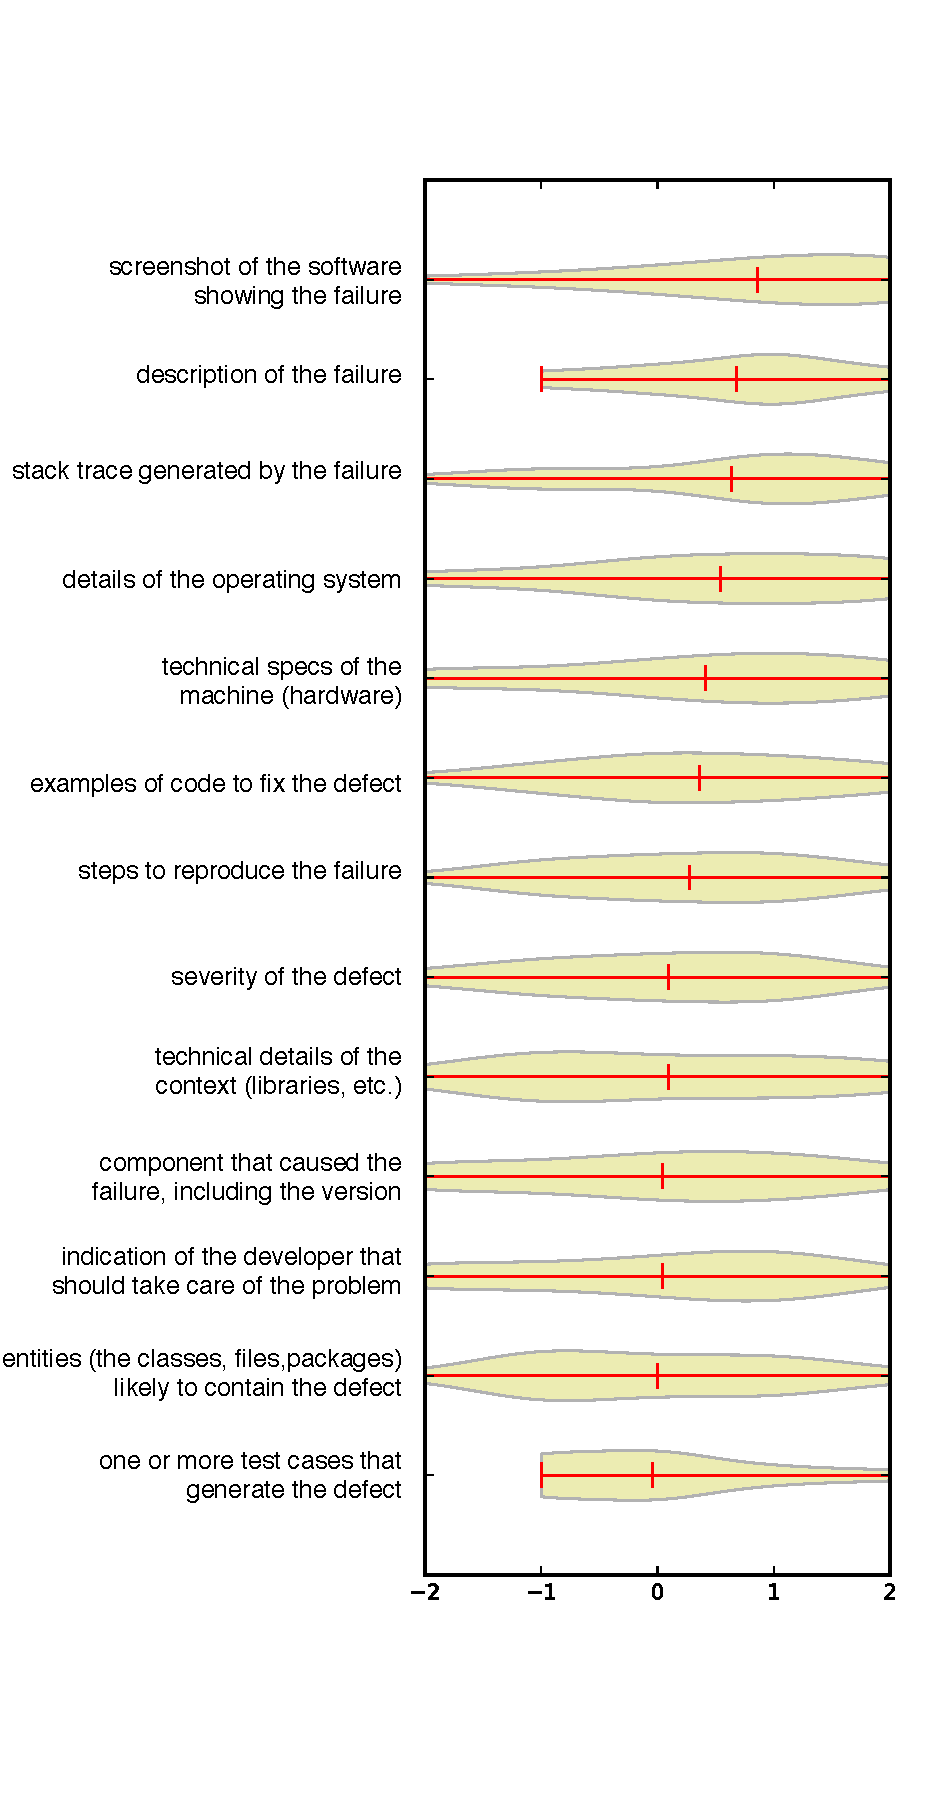
\includegraphics[width=.6\linewidth]{model/survey_plot}
\caption[Survey results]{Survey results: The higher the values, the easier it is to provide the corresponding information, according to the respondents' perception.}
\label{fig:survey}
\end{figure}
%
The majority of the users does not find excessively hard to provide most of the elements.
This is due to the fact that the Pharo community is composed of experienced programmers.
Interestingly, finding the assignee is not considered excessively difficult: Again, this can relate to the community experience, that has a strong core of well-known developers that work as hub when dealing with defects.
The elements considered to be harder to provide are the entity (\eg class, file) that likely contains the defect, the steps to reproduce the failure, and a test case showing the defect.


\subsubsection{Conclusion}

\figref{fig:survey} shows that some elements are perceived as more difficult to provide when submitting a bug report.
There is a set of easier elements, like screenshots, descriptions of the failure, stack traces, and the details of the operating system and hardware.
Those elements are useful in identifying the defect, but are less effective than other elements we identified to support its resolution.


%%%%%%%%%%%%%%%%%%%%%%%%%%%%%%%%%%%%%%%%%%%%%%%%%%%%%%%%%%%%%%%%%%%%%%%%%%%%%%%%%%%%%%
\begin{figure*}[ht]
\centering
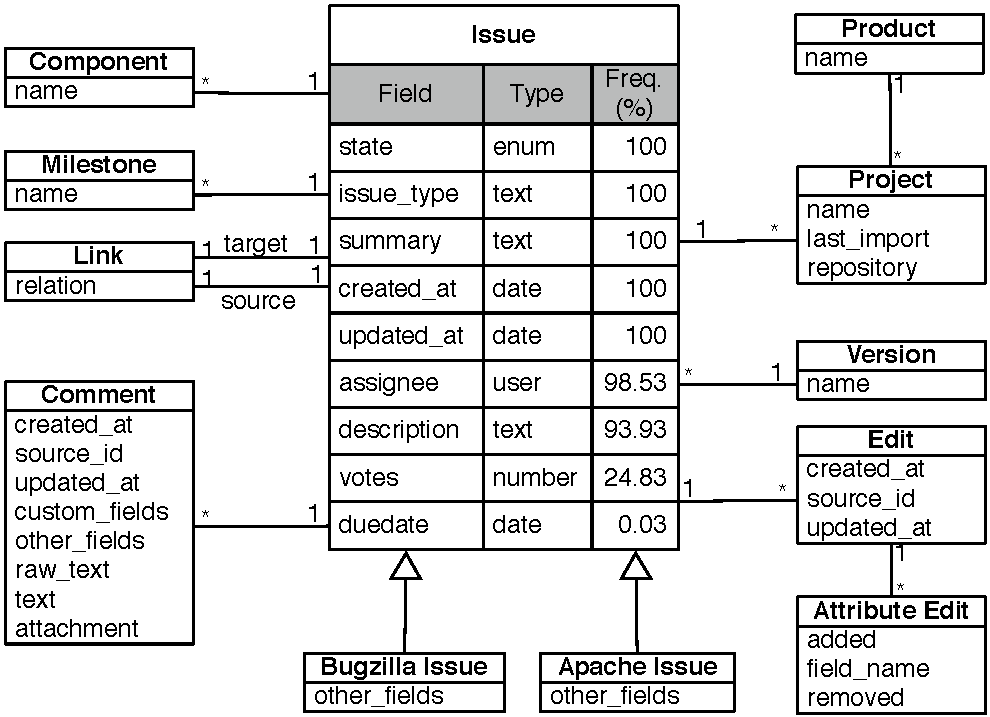
\includegraphics[width=.9\linewidth]{model/model}
\caption{Conceptual diagram of the model of a new bug report}
\label{fig:model}
\end{figure*}

\subsection*{RQ2: What is a comprehensive unified meta-model for describing data from different bug tracking systems?}\label{sec:model-model}

To devise a unified meta-model for the data we collected from the different issue trackers, we extract the model for each separate platform by reverse engineering the data and by using the documentation for the various trackers.
We identify the entities that compose a bug report, the fields  composing it, and the relation between the various entities.
We intersect the list of each bug report and select the most common ones, to summarize the salient traits of a bug report.


\subsubsection{Anatomy of a Report}
Issue trackers are platform independent: They share a flexible common core structure to meet all the possible requirements of a software system's development process.
A bug report is then built around a text description of an issue, where the user can specify the steps to reproduce the issue or include snippets of code that exemplify the context where the issue may happen.

The text description is complemented by additional metadata, used to improve the report and to track the evolution of the bug, and it can also contain attachments, like stack traces and patches.
While the description of the issue and the possibility to attach files is common to all issue trackers, the metadata used to integrate the description differ in each platform.
We can classify these attributes in three layers:

\begin{itemize}[$\circ$]
 \item \textit{Common:} metadata in every report in each platform, \ie the core set of attributes that describes a bug report.
 \item \textit{Platform specific:} metadata that are used throughout a single platform.
 \item \textit{Project specific:} custom metadata set by the users, used in a single project.
\end{itemize}


\subsubsection{The Model}

From the list of entities in a tracker and their list of metadata, we built a model to access the data.
Given our focus, we present a view of the model from the submitter's point of view.
\figref{fig:model} shows the conceptual diagram of the unified model for a typical bug tracking system with the frequencies of use for the common fields and trimmed of the post-report information.
%The diagram is composed of the following entities:


\begin{itemize}[$\circ$]
\item \textit{Issue:} The main entity representing a bug report, with the text description and the metadata provided by the user.
\item \textit{Comment:} User-provided additional information on a report.
\item \textit{Edit:} A change in the existing report.
It can group several changes.
\item \textit{AttributeEdit:} A change to a single element: It contains the modified attribute, the added, and removed text.
\item \textit{Link:} The relation (if any) to another report.
A link maps the connection and defines the type of relation (\eg parent or duplicate).
\item \textit{Project:} The project the issue tracker refers to (\eg Firefox).
\item \textit{Product:} A single instance of an issue tracking platform (\eg Bugzilla or JIRA).
\item \textit{Component:} The area of the code affected by the defect.
\item \textit{Versions:} The software version(s) where the bug was observed.
\item \textit{Milestone:} The software version(s) targeted for a fix, for planning purposes.
\end{itemize}

There are additional attributes that are not present in every platform.
To map these specific elements, there are entities that derive from \textsc{Issue} (\eg \textsc{Bugzilla\_Issue}).

These entities contain the fields \texttt{other\_fields} and \texttt{custom\_fields}.
These are two \emph{dictionary} fields that collect all the fields that are not represented in each model, in an unstructured fashion.
The field \texttt{other\_fields} contains the information from a specific bug tracker, shared in all the projects in that database (like the field \texttt{alias} in \bzilla).
The field \texttt{custom\_fields} contains non standard attributes that are customized by the maintainer of each project.
For example, the attribute \texttt{cf\_status\_firefox41}, of the project \textsc{Firefox} in \bzilla.
Some fields may seem redundant: For example, the field \texttt{updated\_at} of \textsc{Issue} could be derived by the information contained it the \textsc{Edit}s; we tolerate a small degree of duplication of the data, in exchange for flexibility and completeness with different bug reporting systems.



%%%%%%%%%%%%%%%%%%%%%%%%%%%%%%%%%%%%%%%%%%%%%%%%%%%%%%%%%%%%%%%%%%%%%%%%%%%%%%%%%%%%%%

\subsection*{RQ3: What are the recurrent states and transitions in reports?} \label{sec:model-approach-states}

We tracked the evolution of bug reports using the \texttt{state} attribute, which is an enumeration from a set of predefined states.
\tabref{tab:dataset-statuses} shows the states used in the two bug trackers we consider.
Each platform proposes different conventions to map the state of a report.
Often, different projects use the same states in a different context and a different distribution, \eg bug reports in \jira converge toward the \textsc{Closed} state, while in \bzilla they converge toward a state called \textsc{RESOLVED}.
We analyze the state changes by building a transition graph, with an approach similar to the one used by D'Ambros \etal~\cite{DAmb2007b}.

\figref{fig:apache_transitions} and \figref{fig:mozilla_transitions} show the transition diagrams for \jira and \bzilla obtained by the collected data.

\begin{figure*}[t]
\centering
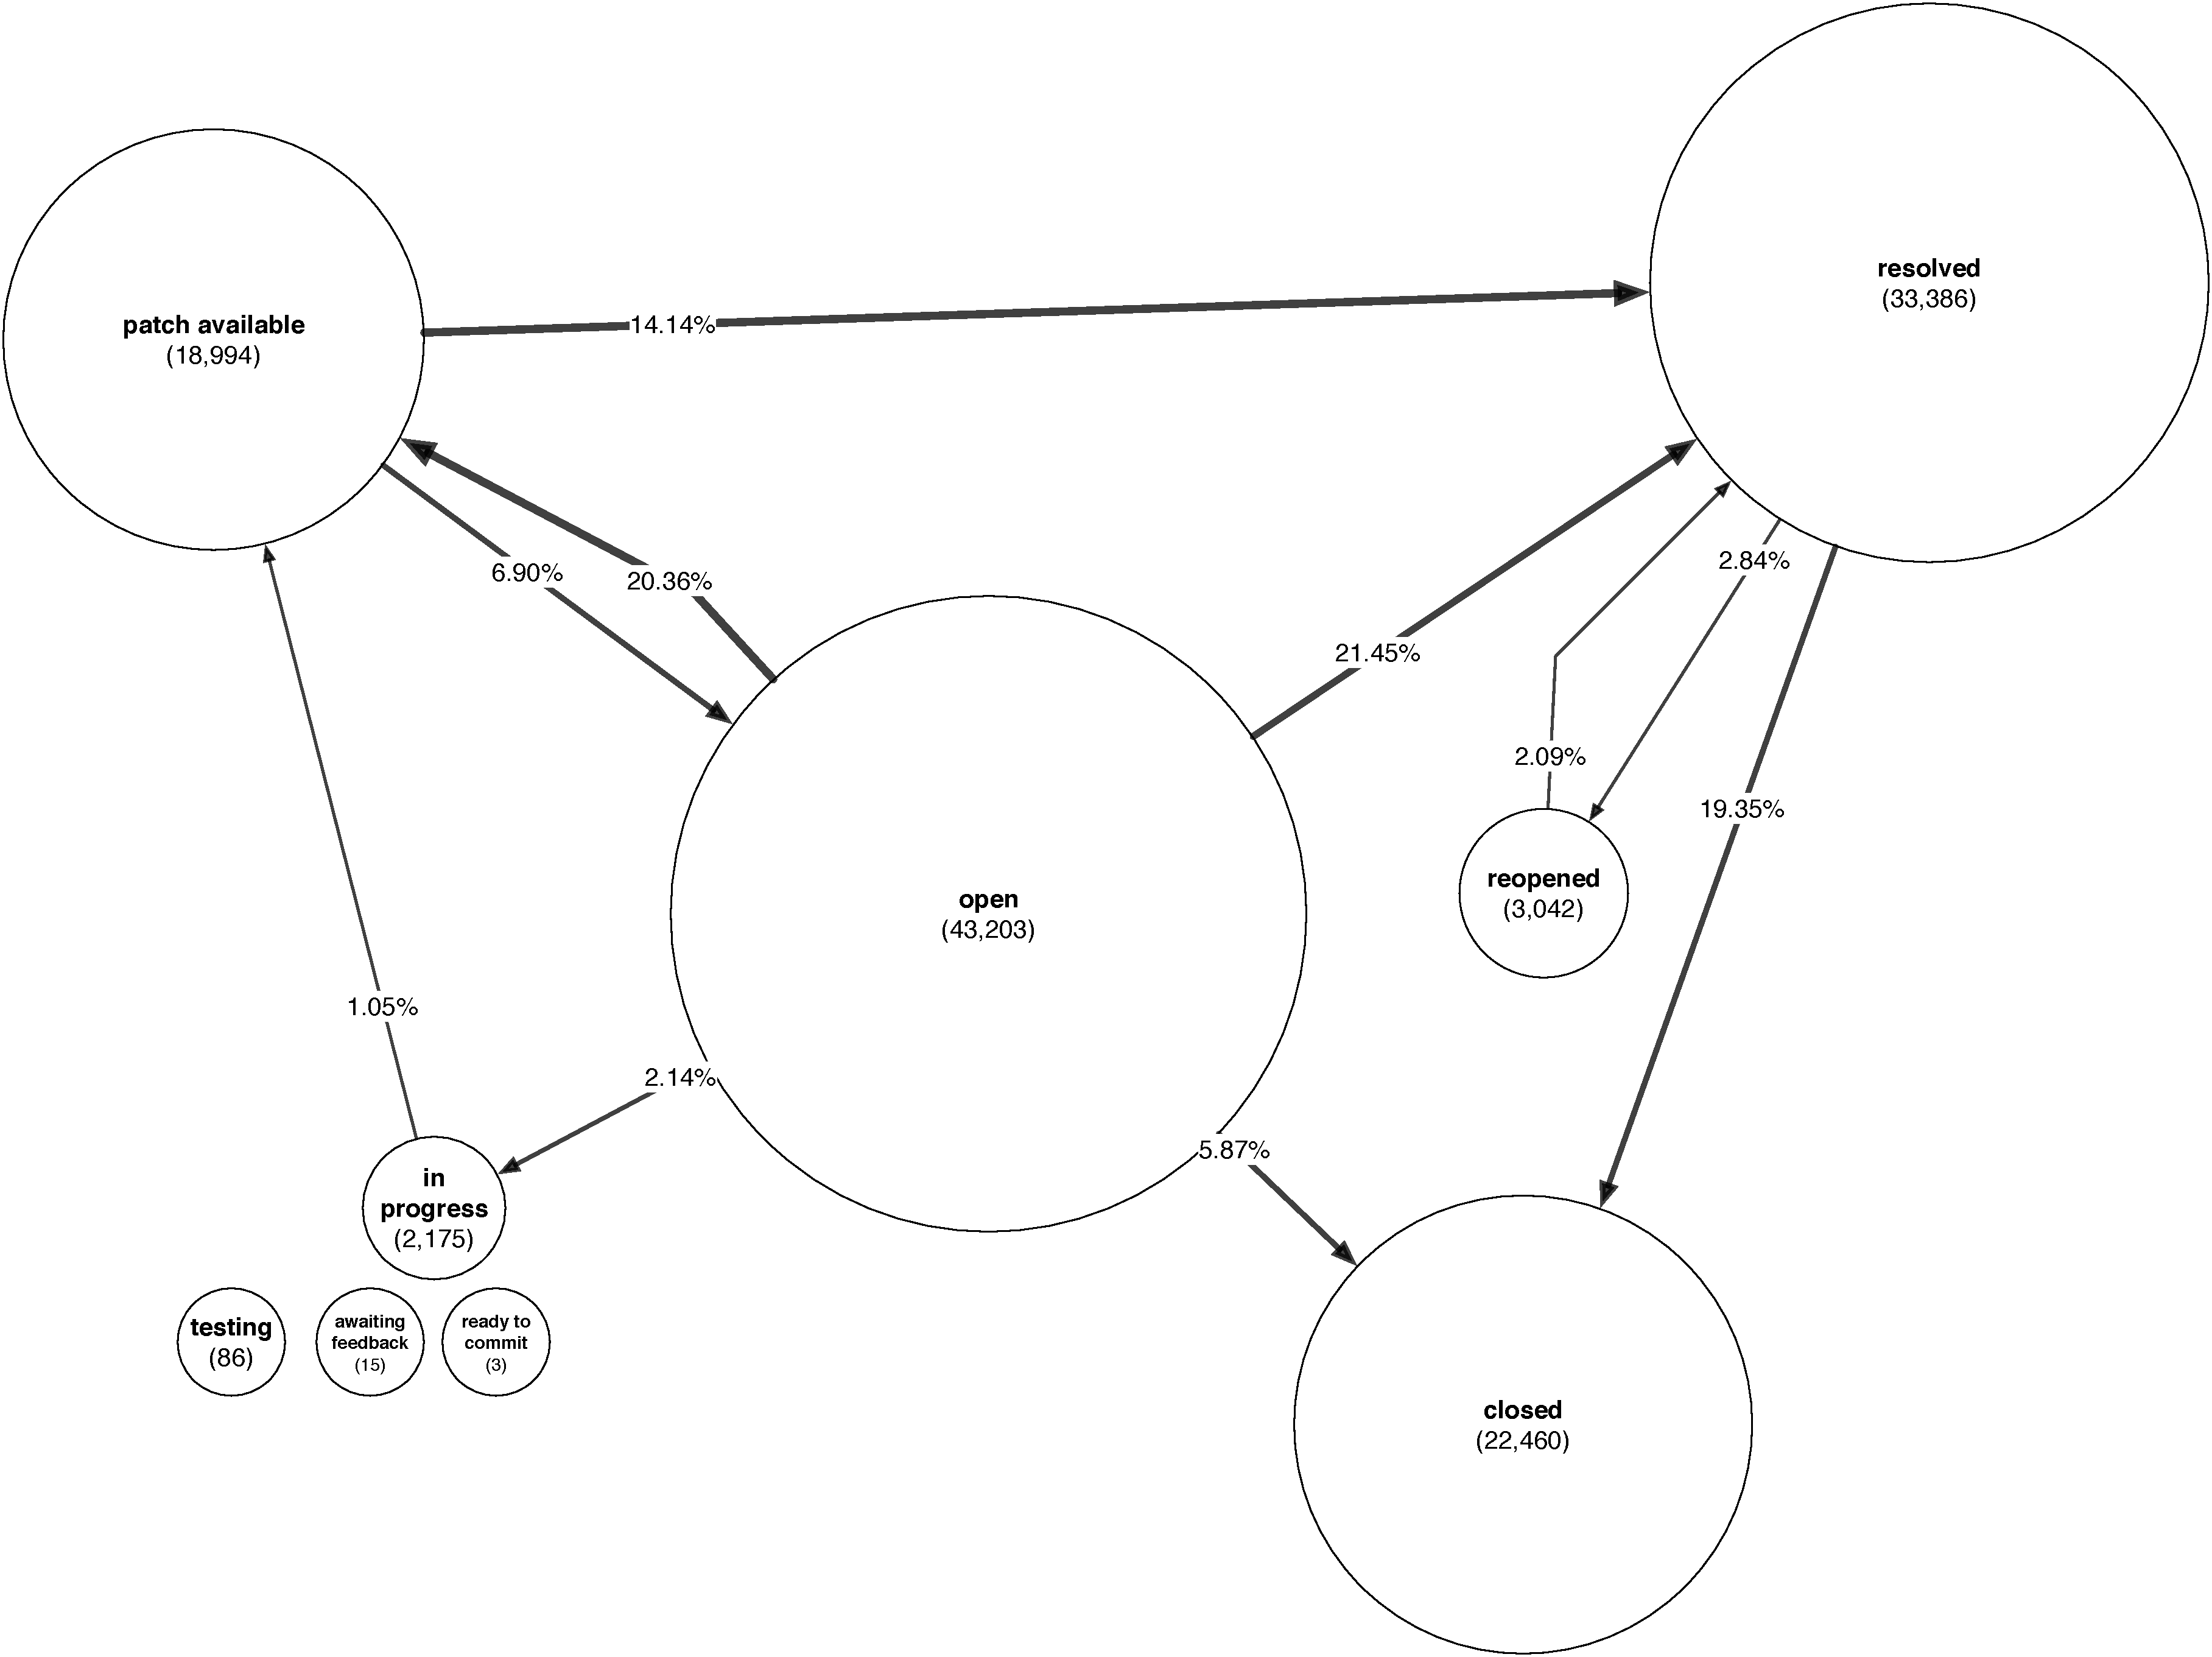
\includegraphics[width=.99\linewidth]{model/apache-transition-diagram}
\caption{Transition graph of all the states in \jira}
\label{fig:apache_transitions}
\end{figure*}

In the diagrams each node is a state, where the area grows with the number of reports that traverse that state, as presented in \tabref{tab:dataset-statuses}.
Each arc between two states indicates a transition from one state to another and its width represents the total number of transitions.
The diagram excludes all edges that make up less than $1\%$ of all the transitions.
Given \figref{fig:apache_transitions} and \figref{fig:mozilla_transitions} we can classify the states in three groups:

\begin{itemize}[$\circ$]

\item \textit{Active states:} The first group contains the most active states (\ie touched by the majority of bug reports), that are often involved in loops between them.

\item \textit{Intermediate states:} These states (\eg \textsc{testing}, \textsc{in progress}, \textsc{reopened}) indicate states where an action is taking place or expected (\eg a patch is waiting for review or the continuous integration server is running the tests).

\item \textit{Unused states:} Some states are rarely used: \textsc{awaiting feedback} and \textsc{ready to commit}.
They represent some corner cases that detail extremely specific aspects of the fixing activity.
Their very low usage may hint at a little interest in tracking these aspects in this way.

\end{itemize}

The analysis highlights that some projects do adopt customized states to track the intermediate aspects of their projects' workflow, but they tend to be not used in practice.

\textbf{Conclusion.} The analysis on the usage of the states in \secref{sec:model-approach-states} seems to suggest that:
\begin{itemize}[$\circ$]
\item A simple model with a few states, as the one described by D'Ambros \etal~\cite{DAmb2007b}, satisfies the need of tracking the state of an issue;
\item Adding customized values to  describe additional specific and intermediate steps in the fixing process is not working to track a better evolution of the state of a report.
\end{itemize}

The latter aspect is strengthened by the fact that \jira offers less states than \bzilla, but these additional states are rarely used in practice.



%\begin{table*}[h!]
%\centering
%\caption{Number of custom fields per project}
%\begin{tabular}{|l|lrrr|}
%\hline
% & \textbf{Project} & \textbf{\# fields} & \textbf{Avg. lifetime (d)} & \textbf{Max lifetime (d)} \\
% \hline \hline
%\bzilla & Air Mozilla & 5 & 154 & 1,004 \\
% & Bugzilla & 5 & 343 & 5,650 \\
% & Core & 142 & 227 & 5,936 \\
% & Firefox & 112 & 235 & 5,314 \\
% & Firefox for Android & 89 & 76 & 2,176 \\
% & SeaMonkey & 90 & 278 & 5,437 \\
% & Thunderbird & 74 & 259 & 5,451 \\
%\hline \hline
%\jira & Cassandra & 11 & 61 & 1,728 \\
% & Hadoop & 13 & 172 & 3,012 \\
% & Lucene & 13 & 182 & 3,787 \\
% & Mahout & 11 & 94 & 1,235 \\
% & Maven & 9 & 402 & 3,443 \\
% & Pig & 11 & 72 & 2,149 \\
% & Sorl & 7 & 148 & 2,858 \\
% & Zookeeper & 12 & 158 & 2,108 \\
%\hline
%
%
%\end{tabular}
%\label{tab:project-fields}
%\end{table*}

%%%%%%%%%%%%%%%%%%%%%%%%%%%%%%%%%%%%%%%%%%%%
\subsection*{RQ4: Does the completeness of standard and project-specific attributes in a bug report relate to its lifetime?}\label{sec:model-fields}

% \AB{It seems strange to me that this section ends here.
% Is the following the actual results on 'custom fields having a measurable impact on the resolution'? It should be in my opinion, so I would recommend having one single section.
% But after reading the next section it is much more than that.
% I think this part and the next subsection should be restructured.
% For example, start from the large lifetime of a report and then investigating the effect of the customized fields.
% This means moving the subsection above near the end of the next one, but not as a separate subsection.}

To investigate the impact that the fields have on solving a defect, we considered the \emph{lifetime} (defined as the time to the final fix) of the closed reports.

In addition to its standard set of attributes, each issue tracker we consider allows projects to define additional fields to customize the structure of a bug report.
In our study, we group all the attributes in three \emph{layers}:

\begin{itemize}[$\circ$]
\item \textit{Core Fields:} The fields that are common to all projects and all the issue trackers.
They map the essential information to describe a software defect;
\item \textit{Tracker-Specific Fields:} The fields that are shared among all the projects in an issue tracker, but are not present in all the platforms;
\item \textit{Project-Specific Fields:} The fields that are customized by the user and appear only in a single project.
\end{itemize}

Each project in our dataset specifies its own set of custom fields.
We also investigate whether these fields have a measurable impact on the lifetime of a bug report.

\begin{figure}[t]
\centering
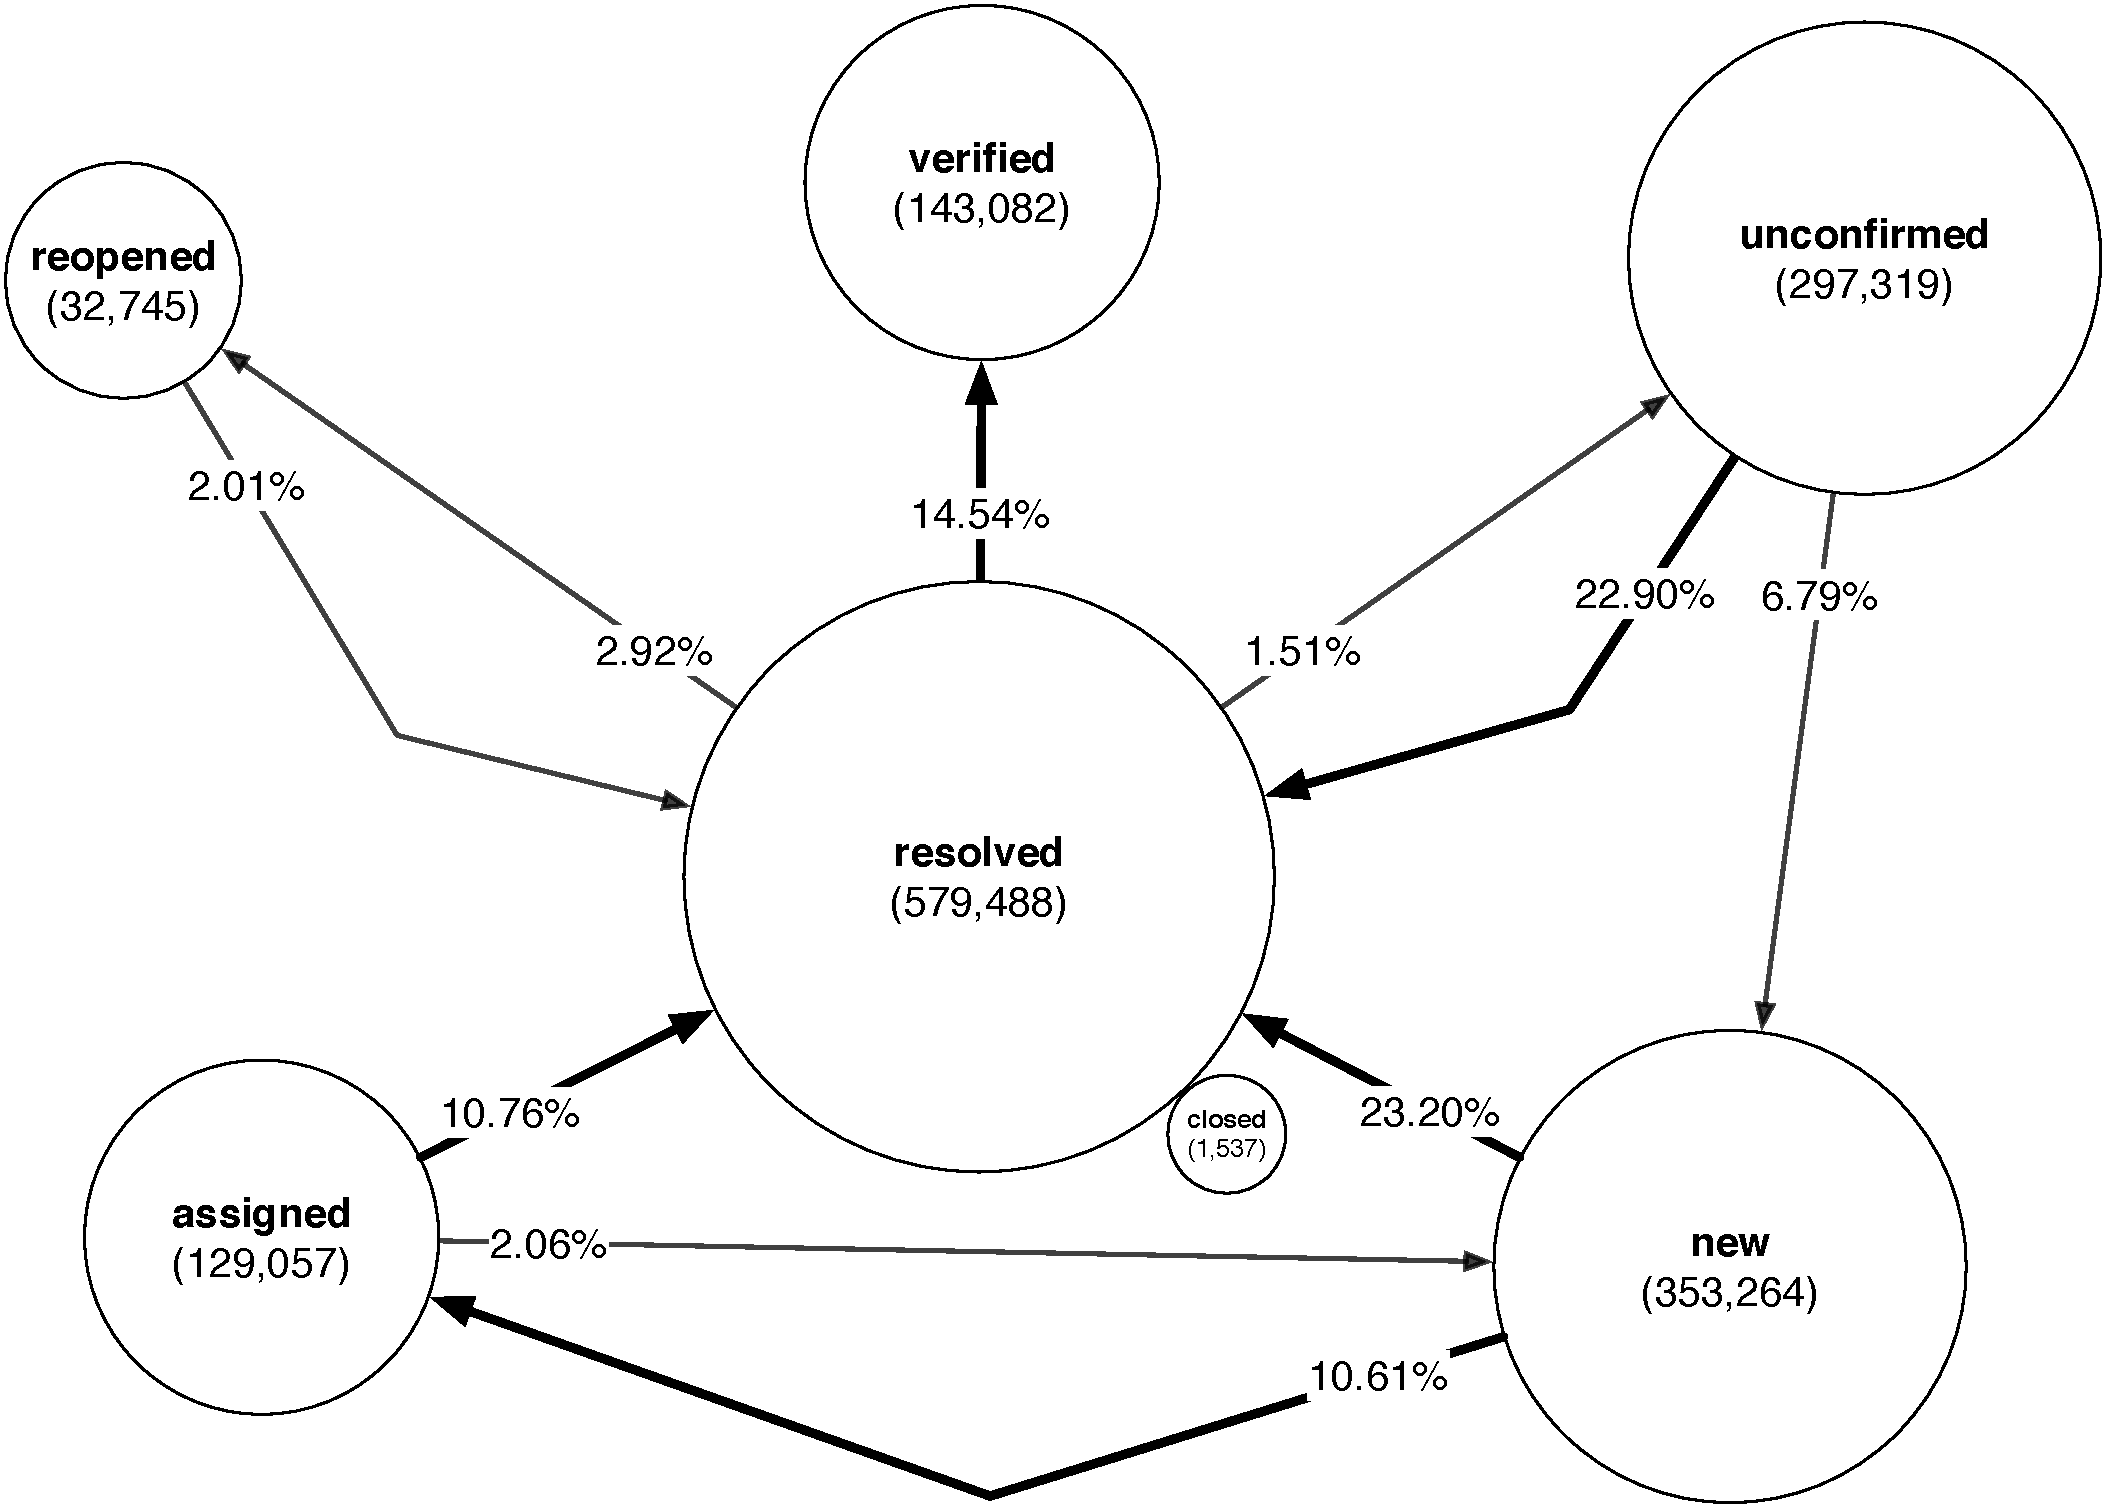
\includegraphics[width=.9\linewidth]{model/mozilla-transition-diagram}
\caption{Transition diagram of all the states in \bzilla}
\label{fig:mozilla_transitions}
\end{figure}

 \tabref{tab:project-fields} shows a count of project-specific attributes in our dataset, including the average and maximum lifetimes of the corresponding bug reports, reported in days.

\begin{table}[ht]\small
\centering
\caption{Number of custom fields per project}
\rowcolors{1}{tablefirstrow}{tablesecondrow}
\begin{tabular}{l|rrr}
\rowcolor{tableheader}\textbf{Project} & \textbf{\# of fields} & \textbf{Avg.
lifetime (d)} & \textbf{Max lifetime (d)} \\
 \hline
Air Mozilla & 5 & 154 & 1,004 \\
Bugzilla & 5 & 343 & 5,650 \\
Core & 142 & 227 & 5,936 \\
Firefox & 112 & 235 & 5,314 \\
Firefox for Android & 89 & 76 & 2,176 \\
SeaMonkey & 90 & 278 & 5,437 \\
Thunderbird & 74 & 259 & 5,451 \\
\hline
Cassandra & 11 & 61 & 1,728 \\
Hadoop & 13 & 172 & 3,012 \\
Lucene & 13 & 182 & 3,787 \\
Mahout & 11 & 94 & 1,235 \\
Maven & 9 & 402 & 3,443 \\
Pig & 11 & 72 & 2,149 \\
Sorl & 7 & 148 & 2,858 \\
Zookeeper & 12 & 158 & 2,108 \\
\hline
\end{tabular}
\label{tab:project-fields}
\end{table}


We now explore the relationship between the various attributes adopted by the different platforms and projects we considered and the effectiveness of a bug report, measured as its lifetime.


\subsubsection{Preparing the data} To interact with the dataset, we created a \emph{vector space model} to allow us to test statistical and machine learning approaches.
Predicting the exact lifetime of a report would be unpractical and unnecessary: a timeframe for the resolution would provide a useful, human-understandable measure, while allowing more accurate predictions.
To introduce such a degree of tolerance, we divide the reports into \emph{buckets} according to their lifetime.

 Using bucketing we can deal with discrete values and adopt a classification approach, as opposed to a regression to predict a continuos variable.
We split the lifetime space into four buckets: less than one day, less than one week, less than one month, and more than one month.
We chose these intervals because they reflect humane time periods and they describe increasing timespans, reflecting that the longer a bug report stays open, the less relevant its exact resolution time becomes.
After bucketing the issues, we model each report as a vector of booleans (each field maps an attribute of the report and its value is 1 iff the user filled it) and associate it with its classification into a bucket of lifetime, which we can feed to different prediction algorithms.


%%%%%%%%%%%%%%%%%%%%%%%%%%%%%%%%%%%%%%%%%
\subsubsection{Principal Component Analysis}\label{sec:model-pca}

To understand the relation between the completeness of a bug report and the fixing time of a defect, we want to inspect how much each field contributes to  the lifetime of a bug report.

For this purpose, we use \emph{Principal Component Analysis} (PCA)~\cite{Abdi2010a} to extract the variance between the different fields.
PCA is a statistical procedure that aims to extract only the salient features from a data table.
PCA transforms the existing data into variables called \emph{principal components}, which are described as a linear combination of the existing features.
The other features are then projected on the principal components.


The components extracted by PCA represent the eigenvectors of the covariance matrix.
Internally, PCA implements a \emph{single value decomposition} to extract the scores of the factors.
%PCA calculates the correlation between the components and projects the instances of the dataset using the components.
The number of components to extract is an open problem, but generally, when solving a correlation problem, PCA keeps the components that have an eigenvalue above the average.

We use PCA to determine which combination of fields carries the most information with respect to the lifetime of a defect, by observing which elements are selected to compose the principal components.
To interpret the results and obtain a general set of fields that influence the lifetime of a bug report, we consider the core fields of the projects.
This operation gives us the important fields that impact the lifetime of a bug report.

After running PCA, we obtain a set of new components that can be used to map the dataset.
We are not interested in the new features per-se, but --- since the features of the dataset are the fields of the bug reports --- we investigate which original features were selected to describe the components.

We then inspect how the components are calculated, obtaining the following selected fields:

\begin{itemize}[$\circ$]
  \item \emph{assignee\_id}: the person the bug report is assigned to;
  \item \emph{creator\_id}: the person that submitted the bug report;
  \item \emph{description}: the number of words in the description of a bug report;
  \item \emph{duedate}: if the bug report has a due date;
  \item \emph{reporter\_id}: the person that initially reported the defect (can be different than the creator)
  \item \emph{summary}: the number of words in the summary of the bug report.
\end{itemize}

These fields were extracted by the algorithm as the most relevant in impacting the lifetime of a bug report.
Although they do not represent the whole amount of information that is needed to describe a software defect, the fact that they were selected by PCA indicates that their contribution in determining the lifetime of a report is significant.
It follows that users and developers should take these elements into account when submitting a bug report and the issue tracker should ensure that these fields are exploited accordingly.

%%%%%%%%%%%%%%%%%%%%%%%%%%%%%%%%%%%%%%%%%%%%%%%%
\subsubsection{Predicting the Lifetime of a Defect} We studied the core fields that are the most relevant in impacting the lifetime.
Now we investigate how the lifetime gets influenced by the different fields defined by each project.
For such an analysis PCA is not suited, as the data is too sparse and the features would be discarded in the process.
We therefore adopt a \emph{machine learning} approach to estimate an approximate lifetime of a bug report given its ``completeness,'' \ie the number of completed fields when submitted.

We verify the impact on the prediction of the different levels of attributes using various machine learning algorithms on our model, by employing the \textsc{scikit-learn} analysis tools~\cite{Pedr2012}.
In particular, we used \emph{Na\"ive Bayes}~\cite{mitc1997}, \emph{Decision Trees}~\cite{mitc1997}, \emph{AdaBoost}~\cite{bish2006}, and \emph{Random Forest}~\cite{brei01} and validated our approach using $k$-fold cross-validation.
We balance the training dataset to get homogeneous buckets containing 50,000 bug reports each, to prevent the different distribution of the sets to give a bias towards the biggest buckets~\cite{bati2004}.
In this context, a random classifier would correctly classify 0.25 of the instances, so a classifier is better than random if it achieves a higher proportion.

\tabref{tab:ml-results} shows the prediction results: Each column represent a classifier, while each row represents each layer of attributes we add to the model.

\begin{table}[ht]\small
\centering
\caption{Prediction results: Proportion of bug reports classified in the correct time bucket, with increment over  random classification (25\% correctly classified bug reports).}
\rowcolors{1}{tablefirstrow}{tablesecondrow}
\begin{tabular}{l|r|r|r|r}
\rowcolor{tableheader} & \textbf{NB} & \textbf{DT} & \textbf{AdaBoost} & \textbf{RF} \\
 \hline
Common & 0.27 (+0.02) & 0.27 (+0.02) & 0.27 (+0.02) & 0.27 (+0.02) \\
+ words & 0.28 (+0.03) & 0.28 (+0.03) & 0.29 (+0.04) & 0.28 (+0.03) \\
+ tracker & 0.36 (+0.11) & 0.36 (+0.11) & 0.42 (+0.17) & 0.36 (+0.11) \\
+ project & 0.37 (+0.12) & 0.36 (+0.11) & 0.42 (+0.17) & 0.37 (+0.12) \\
\hline
\end{tabular}
\label{tab:ml-results}
\end{table}

In the first round we use the \emph{common} attributes displayed in \figref{fig:model}; in the second, we add the number of words that compose the summary and the description of the report; in the third, we add the \emph{tracker} features, \ie the attributes that appear in some issue trackers; in the last, we add the \emph{project} features, \ie the non standard attributes that are customized by the users of the platform.
We follow this order to increasingly add the more and more specific fields and evaluate the impact that the different customizations have on the overall model.
%\AB{why this order? What if I add the last layer first? It would be great to see the real statistical significance (p value?) of each set of attributes, to know which ones really matters.}
We can see from \tabref{tab:ml-results} that the best results are achieved by AdaBoost~\cite{bish2006} using the tracker-specific fields, with an overall accuracy of $0.42$.
Differently from the shared and tracker-specific fields, the project-fields may vary over time.
They are, in fact, constantly added: Firefox, for example, adds a new custom field specific for each release, which happens once every 6 weeks.
This mutability can raise the question whether the contribution of these fields is diluted in such a long timespan.
To mitigate this effect, we recompute our experiments on the subset of bug reports collected in the timeframe that starts exactly one year before the dataset collection.
The new dataset is composed of 31,472 bug reports.
\tabref{tab:ml-results-fresh} shows the results of our second batch of experiments.

\begin{table}[ht]\small
\centering
\caption{Prediction results for bug reports of last year.}
\rowcolors{1}{tablefirstrow}{tablesecondrow}
\begin{tabular}{l|r|r|r|r}
\rowcolor{tableheader} & \textbf{NB} & \textbf{DT} & \textbf{AdaBoost} & \textbf{RF} \\
 \hline
Common & 0.27 (+0.02) & 0.28 (+0.03) & 0.28 (+0.03) & 0.28 (+0.03) \\
+ words & 0.30 (+0.05) & 0.30 (+0.05) & 0.33 (+0.08) & 0.30 (+0.05) \\
+ tracker & 0.34 (+0.09) & 0.37 (+0.12) & 0.46 (+0.21) & 0.39 (+0.14) \\
+ project & 0.35 (+0.10) & 0.39 (+0.14) & 0.46 (+0.21) & 0.42 (+0.17) \\
\hline

\end{tabular}
\label{tab:ml-results-fresh}
\end{table}

Indeed, the results on the most recent dataset do not differ significantly from the results based on much longer timespans.

\textbf{Conclusion.} From our study using PCA, we observe that there exists a set of core elements of a bug report that impact and influence its lifetime.
Comparing these result with the perceived difficulty presented in RQ1, we see that some of these elements, like a description of the problem, the screenshot or the stack trace, compose the description field that we saw impacting the resolution time.
Another relevant element is the assignee of the report, but users find it hard to provide it.
Interestingly, the elements that are the most useful in the resolution of a software defect are also harder to provide.
From the experience with the various issue trackers and their interfaces, we believe that a user submitting a bug report should be offered a clean interface, that minimizes the amount of required information, highlights the most effective elements, and progressively requires the harder or less relevant ones.
The AdaBoost machine learning model achieves the best results, yet it can only predict the lifetime of a limited number of bug reports.
The increment over a random classifier prediction is particularly small for the \emph{common} attributes.
This can be explained by the terse nature of the core model.
Moreover, the \emph{tracker} fields improve prediction, showing a relation between more detailed bug reports and bug lifetime.

After calculating the lifetime of each bug report in the tracker, we compare data from the two considered platforms.
By analyzing the average lifetime of the bug reports in each platform we note that they have a longer lifespan on \bzilla than on \jira, with an average fixing time of 239 and 166 days, respectively.
Even if the longer life of \bzilla projects may explain this phenomenon, we measure a gap between the lifetime of the reports in the two platforms (109 days for \bzilla and 93 days for \jira), even when we restrict ourselves to consider reports submitted after 2009 (\ie when all the projects were active).
There is an interesting, unexplained substantial difference in the way bug reports are processed in the two platforms.
Studies can be designed and carried out to determine whether and how the bug reporting system itself leads to this behavior or there is a possibly unconscious self-selection of projects in using one or the other system.
Concerning project-specific attributes, from the results of the test, depicted in \tabref{tab:ml-results} and \tabref{tab:ml-results-fresh}, it emerges that they have the least weight in predicting the lifetime of a report.
This suggests that they are not related to the fixing time.
This may be a hint that these fields probably track collateral aspects of the evolution of a report that are not related to how quick a bug will be solved.

Last, we examine which fields impact the prediction the most: They are the number of words of the description and the summary, suggesting that an accurate description of the problem is important to engage the developers.
The fields that connect the issue with other reports are also relevant, for example the dependent issues, as well as the fact that a bug report is already assigned at the time of submission.



\section{Discussion}\label{sec:model-discussion}

This section discusses the possible problems of our approach and how our work can be improved.


\subsection{Threats to Validity}

Dealing with large amounts of data can pose some problems in creating an abstraction sufficiently broad to comprise all the aspects of the data, but still specific enough to capture its details.
We spent a considerable amount of time dealing with the representation of the data, extracting its features and cleaning the unneeded parts.
In particular, we carefully excluded from our prediction model all the fields that could yield a-posteriori information on the lifetime of a report.
In a large dataset it is hard, however, to guarantee the complete soundness of the whole corpus, that could contain hidden relations between some attributes.

There is the concern that the lifetime of a bug report, that we used as a measure of quality of a bug report, is not relevant for our task.
However, this metric proved to be an interesting open problem in the field and it represents an interesting heuristic in determining the effectiveness of a report.


\subsection{Next Steps}

Developers tend to prefer simpler models to depict software defects.
Even when provided with customization means, the additional information did not show a correlation with the lifetime of a report.
Modern issue trackers like \jira and \bzilla are complex interfaces over a set of tables in a relational database and the need for additional features over time makes those platforms grow over time, progressively turning them into inflexible \emph{colossi}.

GitHub adopts the opposite approach, by providing a minimal structure of a bug report that is mostly a note attached to a commit or a piece of code.
This interesting approach, however, lacks the descriptive power of the other two platforms.
The need for a simpler model is hinted by the choices of the development team of \bzilla that on version 5.0, released in July 2015, proposes a simplified interface that asks the user for a summary and a description of the problem, polished of all the additional information.

We believe that the future of issue tracking systems lies in flexible structures that can dynamically adapt to different aspects of the development activity.


% %%%%%%%%%%%%%%%%%%%%%%
% \section{Related Work} \label{sec:model-related}
% %%%%%%%%%%%%%%%%%%%%%%
%
% Dealing with bug reports is a non-trivial task: Not only do users have to report meaningful information and developers have to understand and reproduce a problem, but they also have to deal with the large, noisy, and sometimes duplicated  information stored in issue tracking systems.
% To minimize the impact that dealing with reports has on the bug fixing activity, researchers proposed different approaches to support developers and to automate important steps.
%
% \textbf{Reliability of a Bug Report.} The first important aspect involving bug reports is the reliability and completeness of the information contained in a report.
% Through questionnaires, researchers collected information on how developers perceive the quality of a bug report and consider the most influential elements that help understanding a problem~\cite{Zimm2010a,Bett2007,Schr2010a}.
% Researchers also proposed techniques to detect and avoid bug reports that do not contain useful information~\cite{Sun2011}, thus alleviating the developers from information overload.
% Bissyand\'e \etal investigated the impact of the issue tracker on the development of a project~\cite{Biss2013b}, finding that most bug reporters are not developers of the project.
%
% \textbf{Automating Management of Bug Reports.} Researchers proposed different approaches to automate bug report processing~\cite{Weim2006}.
% For example, a crucial aspect of managing bug reports is finding the ideal person to take care of an issue, known as {\em triaging}; Anvik \etal proposed a machine learning based approach to automate this step~\cite{Anvi2006a}.
% Guo \etal conducted a study to predict the aspects that impact the resolution time of \textit{MS Windows} bug reports~\cite{Guo2010}.
% They found that a high number of reassignment of a report decreases the likelihood of the report of being closed quickly.
% They also found that the reputation of the submitter is an important factor to shorten the fixing time.
% Given the expensive nature of the bug fixing activity, Weiss \etal devised an approach to estimate the cost of a bug fix in person-hours~\cite{Weis2007a}.
% Giger \etal studied the issue tracker of different open source project to predict bug fixing time, finding that the assignee and the reporting month are strong predictors~\cite{Gige2010}.
% Also, post-release information like the assignee is useful in increasing the accuracy.
% Bhattacharya and Neamtiu showed the low correlation of current prediction techniques and underlined the need to find additional attributes to increase the confidence of the time estimates~\cite{Bhat2011}.
%
% \textbf{Bug Reports and Social Interactions.} An issue tracker represents also a social aspect of the community: users can interact with developers and provide feedback in fixing a defect.
% Breu \etal performed an analysis on a sample of 600 bug reports, finding that interacting with developers provides help in fixing the defect~\cite{Breu2010}.
% Zhou and Mockus showed that users involved in the development activity, like bug reporting and participating in the community, are more likely to become stable, long time contributors~\cite{Zhou2015}.
%
% \textbf{Bug Report Databases Visualization.} Researchers proposed a number of visualizations to analyze feature of the bug reporting systems.
% For example, D'Ambros \etal performed an analysis of the \bzilla bug repository: They summarized the diagram of the state transitions of a report and proposed a set of visualizations to support the analysis of a bug database at different levels of granularity.
% Their approach allows the user to navigate the history of a single issue tracker and inspect selected part of the system with customized filters~\cite{DAmb2007b}.



%%%%%%%%%%%%%%%%%%%%
\section{Outline} \label{sec:model-summary}
%%%%%%%%%%%%%%%%%%%%

We conducted an investigation to identify the features that are relevant to obtain a \emph{satisficing} bug report.
In doing so, we provided the following contributions:

\begin{enumerate}
\item An overview of the perceived difficulty of submitting elements of a bug report for users;

\item A meta-model for bug reports that represents both the common and specific elements available in reports of different issue trackers;

\item A publicly available dataset of more than 650,000 bug reports, modeled according to our meta-model;

\item An analysis of the contents of the issue trackers, to identify features that are related to reports' lifecycle;

\item Evidence that increasing the number of fields provided when submitting a bug report has little relation on shortening the lifetime of a bug.

\end{enumerate}


This chapter concludes our discussion about collecting information about bugs.
We proposed different approaches to support developers in their bug fixing activity.
We used automation to collect reliable data, we built visualizations to provide effective access to the data, and we discussed how we can improve the model of a bug report.
We are still left, however, with the issue that bug fixing is intrinsically a boring and tedious activity.
In the next chapter we try to mitigate this problem by exploring the field of \emph{gamification}, investigating whether its use can help developers and communities in processing the large amount of unstructured information that populates issue tracking systems.

  %!TEX root = ../tommaso-thesis.tex
%!TEX spellcheck = en_US

\chapter{How to Gamify Software Engineering}\label{ch:gamification}
% \coolchapter{How to Gamify Software Engineering}{}{ch:gamification}


All our efforts up to this moments were aimed at reducing the time spent dealing bug reports by providing tools to access the data in a faster way than just plaintext.
Providing faster and smarter tools solves the problem of reducing maintenance costs, but does little to improve the fundamental issue of engaging developers and contributors.
Software development, like any prolonged and intellectually demanding activity, can negatively affect the motivation of developers.
This is especially true in specific areas of software engineering, such as requirements engineering, test-driven development, bug reporting and fixing, where the creative aspects of programming fall short.
The developers' engagement might progressively degrade, potentially impacting their work's quality.

Gamification, the use of game elements and game design techniques in non-game contexts, is hailed as a means to boost the motivation of people for a wide range of rote activities.
Indeed, well-designed games deeply involve gamers in a positive loop of production, feedback, and reward, eliciting desirable feelings like happiness and collaboration.

The question we investigate is how the seemingly frivolous context of games and gamification can be ported to the technically challenging and sober domain of software engineering.
Our investigation starts with a review of the state of the art of gamification, supported by a motivating scenario to expose how gamification elements can be integrated in software engineering.
We provide a set of basic building blocks to apply gamification techniques, present a conceptual framework to do so, illustrated in two usage contexts, and critically discuss our findings.

\structure

In \secref{sec:gamification-intro} we provide an in-depth introduction to gamification, while in \secref{sec:gamification-principles} we present its principles.
In \secref{sec:gamification-sweng} we introduce a framework for applying gamification to a software engineering context.
In \secref{sec:gamification-evaluation} we propose some guidelines to evaluate the effectiveness of a gamified system, while in \secref{sec:gamification-discussion} we discuss the possible improvements of our work.
Finally, in \secref{sec:gamification-summary}, we summarize and conclude the chapter.

\newpage

% With this paper we make the following contributions:
%
% \begin{itemize}
%
% \item An in-depth discussion of the principles, promises, and perils of gamification (\secref{sec:gamification-principles}).
%
% \item A conceptual framework with which one can gamify software engineering activities (\secref{sec:gamification-framework}).
%
% \item A set of reusable building blocks that serve as a foundation for our gamification framework (\secref{sec:gamification-building-blocks}).
%
% \item A illustration, through several concrete examples and scenarios, of how our gamification framework can be used for the gamification of diverse software engineering activities (\secref{sec:gamification-example-bugs} and \secref{sec:gamification-example-gems}).
%
% \item A critical discussion about our findings and a roadmap for future work in this area (\secref{sec:gamification-summary}).

% \end{itemize}


%%%%%%%%%%%%%%%%%%%%%%
\section{The Rise of Gamification}\label{sec:gamification-intro}
%%%%%%%%%%%%%%%%%%%%%%

Games have been a fundamental part of human civilization for thousands of years.
In 440 BC Herodotus wrote about the Kingdom of Lydia in Asia Minor, where 3 millennia before his time the Lydians invented several games, such as the dice and the ball, to overcome an 18 year long famine.
They would engage in games one day so entirely as not to feel any craving for food, and the next day to eat and abstain from games~\cite{Hero440a}.
While it is unclear whether the story is true, its moral truths reveal the essence of games, which is not escapism, but rather a purposeful and helpful activity to cope with the sometimes adverse or boring reality, which McGonigal goes even as far as to call it a ``broken reality''~\cite{McGo2011a}.

Gamification is defined by Werbach and Hunter as ``The use of game elements and game-design techniques in non-game contexts''~\cite{Werb2012a}.
The concept, not to be mistaken with Game Theory, was pioneered in the 1980s by Richard Bartle, the inventor of the first MUD (Multi-User Dungeon) game, who defined gamification as ``turning something not a game into a game''~\cite{Bart2003a}.

But, what is a game? According to McGonigal~\cite{McGo2011a} all games share four defining traits: a \emph{goal}, \emph{rules}, a \emph{feedback system}, and \emph{voluntary participation}.
The goal gives a sense of purpose.
The rules unleash creativity and foster strategic thinking.
The feedback system provides motivation.
The voluntary participation makes the experience safe and pleasurable.
Suits sums it up with ``playing a game is the voluntary attempt to overcome unnecessary obstacles''~\cite{Suit2005a}.

McGonigal provides several examples of contexts where the performance of subjects has been boosted through gamification~\cite{McGo2011a}.
The contexts range from house holding chores to physical exercise.
While this may seem remote from the software engineering domain, Werbach and Hunter provide an illuminating example closer to our discipline: Microsoft's testing team in charge of the multi-language aspect of Windows 7 invented the Language Quality Game, recruiting thousands of participants who reviewed over half a million dialog boxes, logging 6,700 bug reports, resulting in hundreds of fixes~\cite{Werb2012a}.
Another example is StackOverflow, a popular Q\&A website, where asking and answering technical questions is rewarded with points and badges.
There is evidence that this gamification mechanism is in part responsible for StackOverflow's success~\cite{Vasil2013a}.

Lured by this success, one could be tempted to spread a gamification layer on any kind of software engineering activity.
The questions we answer in this chapter is not only how such a thing can be done in a systematic way, but also whether and when this can lead to a desirable outcome, \ie higher motivation in developers and increased productivity.
First, let us make a small digression in the realm of psychology.
Behaviorism is an approach to psychology that combines elements of philosophy, methodology, and theory.
Its tenet, expressed in the writings of Skinner~\cite{Skin1978a}, is that psychology should concern itself with the observable behavior of people and animals, not with unobservable events that take place in their minds.
Skinner was a firm believer of the idea that human free will is an illusion and that any human action is the result of the consequences of that same action: If the consequences are bad, there is a high chance that the action is not repeated; however if the consequences are good, the actions that led to it will be reinforced.
Put simply, this is the approach ``if you do this, you'll get that''.

Gamification is related to behaviorism, as it is built on the concept of rewards (points, badges, etc.) for specific actions.
However, contrary to the intuition of many, there is substantial evidence that behaviorism does not work: Kohn describes several experiments (for diverse contexts, such as losing weight, quitting smoking, etc.) which revealed that ``token programs show behavior change only while contingent token reinforcement is being delivered.
Removal of token reinforcement results in a return to baseline performance''~\cite{Kohn1993a}.
In essence: When the goodies stop, people go back to acting the way they did before.
Other studies done in schools and work places even brought forth evidence that subjects who were rewarded for doing certain things were performing poorer than subjects who did not receive rewards.

A popular, almost archetypal example of a supposed failure of gamification is the recent removal of the badges and points from the localized search and discovery app Fourquare\footnote{\url{https://foursquare.com}}.
While Foursquare's gamification layer has probably been the cause of its initial growth and success, it was so emphasized that users ended up considering Foursquare just as a game, and not as a business application.
FourSquare's CEO declared that gamification was phased out because of a perception problem of the real purpose of the app itself\footnote{See http://www.gamification.co/2013/03/15/the-removal-of-foursquare-gamification/.
Interestingly, the phasing out backfired, leading to a sensible reduction of the user base growth.}.

How can the success stories mentioned previously be explained, then? Is gamification a lost cause? We believe the answer is no, for a number of reasons.

First, gamification is only partially connected to behaviorism.
A key point is that games represent \emph{voluntary} efforts of the subjects to do something, while behaviorism was conceived as a way to (sometimes forcefully) influence the behavior.

Second, ``simple'' behaviorism is built on fairly tight feedback loops (do this and you get that), while well implemented gamification, such as the one in StackOverflow, has a much longer running time.
Moreover, taking StackOverflow as an example, the presence of an Avatar who is being assigned rewards represents a key ingredient of successful gamification, as we will later see.

Third, and most important, the rewards that come out of successful gamification are not of a venal nature, but according to McGonigal they fall into four categories, that in conjunction represent ``the foundation for optimal human experience [..], they're the most powerful motivations we have other than our basic human needs (food, safety, and sex)''~\cite{McGo2011a}.
These four categories are \emph{satisfying work}, the \emph{experience/hope of being successful}, a \emph{social connection}, and a deeper \emph{meaning}.
We will discuss these aspects in the coming sections.

Summing it up, gamification is not about rewarding people with trinkets and tokens, it is about enriching their activities with ``gameful'' aspects.
As this represents a fairly novel field, we have performed an in-depth investigation of the topic~\cite{Mast2014a}, which we distill here into a systematic approach for the gamification of software engineering.

With this chapter we make the following contributions:

\begin{itemize}

\item An in-depth discussion of the principles, promises, and perils of gamification (\secref{sec:gamification-principles}).

\item A conceptual framework with which one can gamify software engineering activities (\secref{sec:gamification-framework}).

\item A set of reusable building blocks that serve as a foundation for our gamification framework (\secref{sec:gamification-building-blocks}).

\item A illustration, through several concrete examples and scenarios, of how our gamification framework can be used for the gamification of diverse software engineering activities (\secref{sec:gamification-example-bugs} and \secref{sec:gamification-example-gems}).

\item A critical discussion about our findings and a roadmap for future work in this area (\secref{sec:gamification-summary}).

\end{itemize}


%%%%%%%%%%%%%%%%%%%%%%%%%%%%%%%%%%%%%%%%%%%%%%%%%%%%%%%%%%%%%%%%
\section{Games and Gamification} \label{sec:gamification-principles}
%%%%%%%%%%%%%%%%%%%%%%%%%%%%%%%%%%%%%%%%%%%%%%%%%%%%%%%%%%%%%%%%

First, we discuss the principles of game design (\secref{sec:gamification-principles:games}) and gamification (\secref{sec:gamification-principles:gamification}).
This will help us to understand how the obtained background can be leveraged to apply gamification in software engineering.

%%%%%%%%%%%%%%%%%%%%%%%%%%%%%%%%%
\subsection{Why Do We Play Games} \label{sec:gamification-principles:games}

The  idea that games can be adapted to positively influence tasks and activities in other domains is older than the term \emph{gamification}, which only gained popularity in the recent years.

In 1980, Malone~\cite{Malone1980} studied what makes computer games captivating to extract the features that can be used to support teaching.
He considered two types of motivation: \emph{extrinsic motivation}, triggered by means of a {\em reward}, and \emph{intrinsic motivation}, triggered by the {\em satisfaction} of performing an action.
Malone identified three main elements that influence the engagement in a game:

\begin{enumerate}[(a)]

\item\textbf{Challenge} introduces uncertainty through hidden information, randomness, cognitive limitation of players, and variable difficulty.
Self-contained and small goals are better than long term ones at sustaining performance and interest in an activity.

\item\textbf{Fantasy} refers to the mental images of things and situations out of the actual experience of the player.
Malone discerns two types of fantasies: Extrinsic fantasies that depend weakly on the skills used in a game, and intrinsic fantasies that the player feels while using a particular skill in the game.

\item\textbf{Curiosity} arises from incomplete or contradictory knowledge.
Sensory curiosity regards the attraction toward changes in the environment, while cognitive curiosity concerns the expectation of reaching a higher level of cognitive structures.

\end{enumerate}

Building on Malone's work, Gee~\cite{Gee2003} identified 36 learning principles crucial in video games and learning contexts, which we present in summarized form to identify the salient traits:

\begin{itemize}

\item\textbf{Learning Process:} the learner creates a mental model of the domain, and probes it to test her knowledge.
The cycle of creating hypotheses and testing them is a crucial element of games and learning processes, and is present in humans already at the infancy stage.

\item\textbf{Sources of Knowledge:} Learners acquire knowledge through several modalities including images, words, sounds, symbols, interactions, abstractions, \etc All this leads to an enrichment of the person playing.

\item\textbf{Path to Competence:} Learners reach some achievements for which they receive intrinsic rewards, which also works as feedback.
The learning process is performed slightly outside the comfort zone of the learner, so that the learner perceives the activity as ``challenging but not unfeasible''.
This connects to the concept of ``Flow'', defined by Csikszentmihalyi~\cite{Csik1990a} as the mental state of operation in which a person performing an activity is fully immersed in a feeling of energized focus, full involvement, and enjoyment in the process of the activity.

\item\textbf{Safe Environment:} The environment where leaners operate is designed to keep low risks for each action, to allow exploring without facing serious consequences.
In essence, dying in a game is not a bad thing, because it usually leads to learning.
Moreover, the environment is disclosed gradually, to let the learner discover new parts of the subject domain, thus also feeding curiosity.

\item\textbf{Learning Progress:} The process of learning begins with a simplified image of the real domain.
What the apprentice learns in earlier steps leads to abstractions of the concept that she can use again in similar situations.
Learners build their knowledge ``bottom-up'', starting from basic skills, and making up hypotheses when a more complex case shows up, exploiting what they previously found.
This feeds again curiosity and reinforces self-confidence.

\end{itemize}

In ``Reality is Broken''~\cite{McGo2011a} McGonigal suggests that the use of game elements can help making daily life and reality more interesting and engaging.
She defines games as a combination of a goal, rules, feedback and voluntary participation; this makes games perfect environments to (im)prove our own capabilities.
Pushing our skills to their limit, and then some more, means ``producing hard work'', and provide a sense of achievement that is the exact opposite of depression.
The immersion created from voluntary work can improve the mood for hours or days, ``because when the source of positive emotion is yourself, it is renewable''~\cite{McGo2011a}.
McGonigal identifies four crucial elements that should be craved to achieve happiness: satisfying work, hope of being successful, social connection, and meaning.
The use of games elicit positive participation towards a common interest, thus helping the development of communities.
To improve the engagement in reality, she proposes a \textit{sustainable engagement economy} built around intrinsic rewards.
She defines \emph{collaboration} as the sum of three types of concerted effort: cooperation (acting voluntarily toward a common goal), coordination (synchronising activities and resources), and co-creation (producing a result together).

Massively multi-player online games are illuminating embodiments of this concept: Even when competing for resources, the players constantly collaborate in the definition of the game world.
McGonigal also proposes the idea that different affinity groups can collaborate and give value to the different qualities of each community, to create a \emph{superstructure} that is able to solve problems that each single group would not be able to tackle.
``A superstructure brings together two or more different communities that do not already work together.
A superstructure is designed to help solve a big, complex problem that no single existing organization can solve alone.
A superstructure harnesses the unique resources, skills, and activities of each of its subgroups.
Everyone contributes something different, and together they create a solution''~\cite{McGo2011a}.

In essence, games enrich gamers and provoke positive emotion, which, if leveraged, help to structure experience and provide a powerful tool for inspiring participation and motiving hard work.

%%%%%%%%%%%%%%%%%%%%%%%%%%%%%%%%%%%%%%%%%%%%%
\subsection{Gamification: Principles, Promises \& Perils} \label{sec:gamification-principles:gamification}

Werbach and Hunter summarized the positive effects of a well designed gamification system as~\cite{Werb2012a}:
\begin{inparaenum}[i)]
  \item \emph{Inherent relatedness}, \ie being part of something bigger than ourselves;
  \item \emph{Rewards for doing good}, \ie doing activities that are self-rewarding;
  \item \emph{Behaviour change}, \ie getting people doing something that they did not use to do or they did not engage in, changing their habits.
\end{inparaenum}

According to Huizinga~\cite{Huizinga2006}, there is a virtual line that separates the game world from the real world.
When a person is in this \emph{magic circle}, the game rules matter over the rules of the real world.
The purpose of gamification is to put the user in the magic circle, emphasizing the attitudes of voluntariness, learning, problem solving and exploration.

The most common form of feedback used in games is the \emph{PLB Triad}, where \emph{PLB} stands for Points-Badges-Leaderboards.
Points, Badges, and Leaderboards are also widely used in gamification systems, because they appear to work moderately well as extrinsic motivators.
To introduce a gamification layer on a real or virtual system, the first step is to understand whether there are the right assumptions to make it successful, which Werbach and Hunter~\cite{Werb2012a} identified as:

\begin{itemize}
  \item \textbf{Motivation:} Where to derive value from to encourage a certain behaviour?
  \item \textbf{Meaningful Choices:} Are the target activities sufficiently interesting?
  \item \textbf{Structure:} Can the desired behaviors be modeled through algorithms?
  \item \textbf{Potential Conflicts:} Does the game avoid tension with other motivational structures?
\end{itemize}

This schema must be considered in every phase of the gamification of a system, and used to verify the ideas that survive the review process.
Depending on which game dynamics and techniques the game designers exploit, a gamified system takes a particular shape, often in the following forms:
\begin{itemize}
\item \textbf{Inducement Prizes:} They define a competitive game environment concretized into a contest to motivate efficiency, creativity, and flexibility.
Prizes can assume several forms, where the PLB Triad is most frequent.
\item \textbf{Collective Action:} This is a collaborative game context where people come together and accomplish a task.
The main requirement is that the tasks can be split up to exploit ``crowd sourcing''.
\item \textbf{Virtual Economies:} Small, complete and structured economies that arise in virtual worlds.
A well-known example comes from loyalty programs (like the ones of supermarket chains).
The risk of crossing the line between virtual and real economies is often underestimated.
\end{itemize}

Adopting a gamification system means modifying the behavior of people and influencing their routine, which, as we have seen in the introduction might actually backfire.
As such, it represents a delicate matter that may negatively impact well functioning parts of the system.
Put simply: Adding a reward to a boring task may help to motivate the user, but will not turn it into an engaging activity.

Similarly, gamifying an already interesting activity may move the focus from the activity itself to the reward system.
For example, Grant and Betts~\cite{Grant2013} carried out a study on the behavior of Stack Overflow users, and showed that many new users work intensively to acquire the easiest badges as quickly as possible, with increased user activity  immediately before the awarding of a badge and a strong activity decrease in the period afterwards.

In general, gamification succeeds at the workplace only when it is well designed and the employees truly consent to it.
Also, it was discovered that the most reliable predictor of consent to Gamification comes from the fact that employees are used to play games in their free time or not: A person used to gameplay has less difficulties in embracing the experience of the game, catching its rules, and engaging it~\cite{mollick2013mandatory}.

Alfie Kohn raised serious concerns about the use of reward systems and virtual economies in education and the workplace~\cite{Kohn1993a}.
He argues that rewarding a certain behavior educates the user towards obtaining the specific reward, hiding the actual goal of the task.
It is also possible that the users perceives the rewards as a controlling mechanism, thus generating repulsion instead of engagement.
While this is a crucial aspect to consider, we believe it is still possible to successfully use gamification to improve a system.
If we consider the StackOverflow example, the points obtained by answering a question are used to build a reputation system that is used through the platform to identify experts.
At the same time, the points awarded are subject to a quality review from the users, who concur in the evolution and the quality of the platform.
As such, if gamification is used to enrich existing interactions, rather than to force users to perform boring actions, it can be a valuable tool in growing a successful community.

The last set of perils we discuss are of a legal and moral nature, but not necessarily connected to the professional world.
First, there is the question of {\em privacy}, as gamified systems and contexts can be misused to collect a vast amount of information about the players.
Second, as stated by Bogost\footnote{See \url{http://www.gamasutra.com/view/feature/134735/persuasive_games_exploitationware.php} } in an essay entitled ``Exploitationware'', gamification might induce people to do things that are not really in their interest, \ie proposing to ``replace real incentives with fictional ones.
Real incentives come at a cost but provide value for both parties based on a relationship of trust.
By contrast, pretended incentives reduce or eliminate costs, but in so doing they strip away both value and trust.'' Third, gamified systems can be easily tweaked to implement deceptive marketing and advertising.
Last, but not least, since players spend vast amounts of time and effort in building up their avatars/personas, they conceptually ``own'' them, which in turn might lead to unforeseen issues about property and ownership.
This constitutes a new area of law, further complicated by its borderless nature.

Overall, gamification is a double-edged sword, but it is a rising phenomenon, which must be better understood to leverage its great potential.



%%%%%%%%%%%%%%
\section{Gamifying Software Engineering: (Not) An Easy Game?}\label{sec:gamification-sweng}
%%%%%%%%%%%%%%

We use a concrete running example to explain why gamifying software engineering areas is far from trivial.
The running example is the one of bugs, in terms of reporting, tracking, and fixing them.
Bug tracking systems (also known as issue trackers) are being used to store and manage bug reports since decades now.
In short, developers and users use them to report new bugs they encountered, by providing data about the encountered bug, the situation in which it came up, etc.
They report those bugs using web-based systems, such as Bugzilla and Jira.
Developers then take up the bug report, try to understand it also by reconstructing the context, and then provide fixes and patches that hopefully correct the reported bug.
Despite their many benefits, modern bug trackers are far from perfect, and suffer from redundant reports, incorrect data, and in general a poor quality of the bug reports, as pointed out by a number of researchers~\cite{Bird2009a,Zimm2010a}.
Moreover, open source communities suffer from lack of participation by the users in this context.
For example, at the time of writing, the Mozilla Firefox\footnote{https://bugzilla.mozilla.org/} bug tracker contains ca.
20,000 open bug reports of which over 90\% have not been assigned to anyone.

Enter gamification.
How can it be used to ameliorate the situation, and can it be used to increase participation from the community as well as lead to higher quality reports?

A seemingly simple approach is to spread over bug trackers a layer of points and badges, and every week post leaderboards with the most active reporters and fixers.
We believe that such an endeavour would at the beginning be successful, and probably there would be an increased participation of people.
However, soon enough what gamers call ``pointsification'' would kick in, which is the focus of players on the rewards (the points, the badges) and not on the actual (technical and intellectual) achievement that led to the rewards.
Put simply, soon enough there would be users who would start reporting non-existent bugs just to notch up their leaderboard ranking.
This would lead to a situation, similar to the one observed in StackOverflow by Grant and Betts, where people would stop reporting/fixing certain bugs as soon as they obtain the corresponding achievement.
The pun being intended, it would be ``game over'' for such a gamification approach.

The real goal of gamification has to be a different one, namely to improve the organization of the community, by helping and stimulating experts, by highlighting important bug reports, by making visible important achievements such as the closing of a difficult bug report, and in general by fostering and maintaining motivation over a longer period of time.

We need an approach which supports what McGonigal~\cite{McGo2011a} identified as the 4 key aspects of gamification: {\em Satisfying work}, the {\em experience/hope of being successful}, a {\em social connection}, and a deeper {\em meaning}.
Next, we present our framework for the gamification of software engineering, which we distilled from a vast literature review~\cite{Mast2014a}.
Due to space constraints we discuss and present only the salient underlying theory.



%%%%%%%%%%%%%%%%%%%%%%%%%%%%%%%%%%%%%%%%%%%%%%%%%%%%%
\section{Software Engineering Gamification Framework}\label{sec:gamification-framework}
%%%%%%%%%%%%%%%%%%%%%%%%%%%%%%%%%%%%%%%%%%%%%%%%%%%%%

Our framework is an extension of Taje's layered approach to game design\footnote{\url{http://www.gamecareerguide.com/features/355/gameplay_deconstruction_elements_.php}}.
Taje lists six layers, from lowest to higest, named Token, Properties, Dynamics, Goal, Meta, and Psycho.
Game design elements can be mapped into the six layers and interact with each other by means of interactions.
Our goal is not to describe Taje's approach here, but to describe our framework.
The reason is that Taje's approach targets game design in general, while our framework targets gamification and in particular software engineering gamification.
In essence, Taje's layers are a subset of the components of our framework.

\begin{figure}[ht]
\centering
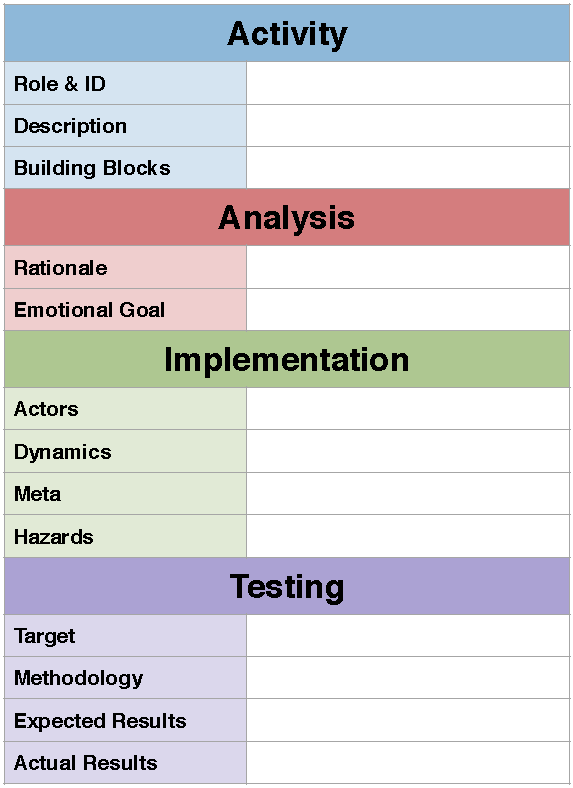
\includegraphics[width=6cm]{gamification/frame2}
\caption{Gamification Activity Template}
\label{fig-frame}
\end{figure}

Our framework is based on the concept of {\em Activity} (depicted in \figref{fig-frame}), which is composed of {\em Analysis}, {\em Implementation}, and {\em Testing}.
Each activity pertains to a specific user type (role), present in gamification systems, which can be \begin{inparaenum}[i)] {\em \item Observer}, who acts in read-only mode and does not contribute anything new, {\em \item Writer}, who only interacts by modifying existing contents and {\em \item Solver}, who accomplishes the objectives of the gamification system\end{inparaenum}.
People interacting with a gamification system dynamically switch between these roles.

An \textbf{Activity} consists of an {\em ID} formed by the initial letter of the role plus an incremental number (\eg the first activity listed in Writer has the ID ``W1''), a brief {\em description}, and a list of pertinent gamification building blocks (which we describe later).
Each activity is structured in the following way:

\begin{enumerate}

\item{\textbf{Analysis:}} Each activity within the gamification environment must come with an easily understandable {\em rationale} to connect to the global objectives of the environment, and the {\em emotional goal} we want to achieve in the people.
Without this analysis step, a gamification effort risks turning into a random set of arbitrary decisions.

\item{\textbf{Implementation:}} To implement an activity the {\em actors} must be known and we need to understand which gamification {\em dynamics} they will be involved in, which represent the tactics to engage people in a specific activity.
This is instantiated with game components we call {\em meta}, following Taje's nomenclature.
Last, one must ponder the {\em hazards} that can arise from a game structure (algorithmic issues, misbehavior, hardware requirements, \etc).

\item{\textbf{Testing:}} The last component is devoted to testing the activities, where it must be understood which entities are the {\em target} of the testing, which {\em methodology} can be used to perform the testing, and lastly, which the {\em expected results} and the {actual results}, to facilitate an iterative approach to the development of a gamification environment.

\end{enumerate}

This description of the framework is given from a conceptual point of view, obtained through several iterations and pilot tests we do not describe due to space constraints.
Before we can provide concrete examples of how the framework is to be used, we need one last missing and fundamental piece: Each activity hinges on one or more {\bf building blocks}, which also denote the particular categories of gamification it belongs to.

%%%%%%%%%%%%%%%%%%%%%%%%%%%%%%%%%%%%%%%%%
\subsection{Gamification Building Blocks}\label{sec:gamification-building-blocks}

The ten building blocks we present here have been identified during the construction of several software engineering gamification environments we have constructed, and which we briefly present in a latter section.
We do not claim the list of building blocks is exhaustive, but after constructing the aforementioned gamification environments we did not see other building blocks emerge from our efforts.
The building blocks are denoted by a series of aspects recurrent in the literature: According to Werbach and Hunter players {\em go through a journey}, progressing through an environment, first by ``on-boarding'', then by ``scaffolding'', and later by achieving ``mastery''~\cite{Werb2012a}.
Adopting Lazzaro's ``keys to emotions''~\cite{Lazzaro2004}, good emotions triggered by solving puzzles, accepting challenges, and designing strategies are elicited by {\em hard fun}.
Moreover, the {\em people factor}, which stems from socializing and working with people and giving/receiving gratitude is fundamental in community-based gamification environments.
Embracing Seligman's concept of {\em resource building}~\cite{seligman2000positive}, it is beneficial to provide some form of avatar of the player which matures and grows as the gamification environment is being explored.
This in turn is tied to the concept of ``leveling up'' described by McGonigal~\cite{McGo2011a}.

Before coming to the ten building blocks, one further consideration: As opposed to existing gamification environments, one which is tailored for software engineering must include the possibility of dynamically adapting itself.
Since software systems are developed for very long periods of time, even decades, an environment should feature the possibility of removing existing rewards and adding new ones as the environment is being used.

\buildingblock{Portal}{portal} When users cross the boundaries of the gamified platform, they register a profile and provide information that describes them to the virtual community.
Despite being a trivial operation, it has a relevant feature: It is the very first action that users accomplish in entering the new world, and should be acknowledged with a reward.
{\em Example:} Bob registers to the Bug Tracker and receives a ``Welcome'' badge.

\buildingblock{Production}{production} After registering, users must become immediately productive in the environment, because delays in starting using the platform may result in a drop of interest and cause users to quit.
We split this block into three sub-blocks, according to the ways in which users have the possibility to produce content and receive rewards.
\begin{itemize}
  \item \textbf{Symbiosis}: performing an activity that directly or indirectly helps someone else's activity or state.
Acting well in favour of others benefits both parties.
{\em Example:} Bob provides useful comments to a bug being handled by someone else.
  \item \textbf{Narcissus\footnote{Narcissus was a Beotian hunter in Greek mythology who was so proud of his feats that he fell in love with his own image reflected in a pool.}}: doing something to self-improve one's position in the community.
This action helps users to understand the structure and  mechanisms of the community.
{\em Example:} Bob provides his first bug fix.
  \item \textbf{Hive}: proposing an idea to improve the platform and community life.
{\em Example:} Bob proposes to introduce a ``Bug of the day'' notification mechanism.
\end{itemize}

\buildingblock{Bravery}{bravery} In the production process, users may attempt hard tasks.
The more skilled they become, the more confidently they will attempt to achieve bigger goals.
Such bravery leads to important achievements and should be equally rewarded.
{\em Example:} Bob fixes an old bug that made many people despair and is awarded by the community with an ``Unstoppable'' badge.

\buildingblock{Scrum}{scrum} In Rugby, Scrum is a way of restarting the game: Players bind together in order to make the other team collapse and take possession of the ball.
The key is to rely on the strengths of everyone.
Cooperating, collaborating, sharing useful tools, competing against, socializing with other community members is intrinsically motivating.
The system should reward and promote teamwork.
{\em Example:} Bob spends time assigning bug reports to users that he knows to be expert in the area, or tagging easy bugs for newbies.

\buildingblock{Chameleon}{chameleon} While gaining skills and experience, the user may do something unique, spectacular, or never tried before.
The environment should react by introducing a new achievement and release an ad-hoc reward, which becomes part of the gamification library of the system and achievable by other users.
Conversely, if a specific reward has never been reached by any user for a long time, the reason might be its impracticability; the system should dynamically remove such an achievement from the library.
We affiliate such a dynamism with the ability of chameleons to change their own skin colour according to the surrounding environment.
{\em Example:} Bob closes five bug reports with a single fix.
The system administrators create a special ``Epic'' badge, and add it to the possible badges users can achieve.

\buildingblock{Thunderbolt}{thunderbolt} When users become experts, with many obtained rewards, they might fall into a state of boredom.
The result is decreased motivation and productivity.
To awake them from inactivity, the system should hit them like a thunderbolt with an announcement and direct them toward a new challenge, such as a one-week long quest where contestants can be awarded custom prizes.
This should spur many users to participate.
{\em Example:} Bob has not participated in any bug fixing activity for the last month.
He and similar users are notified about a complex bug and a bounty for fixing that bug.

\buildingblock{Phasing}{phasing} Users may perform actions in the virtual world that, in reality, produce a permanent impact on the surrounding.
Phasing suggests to mutate the environment according to the progression of each user's expertise.
Two users, at different stages of their progression  see different representative phases of the same scenario and can interact with it in different ways.
{\em Example:} Bob tags bugs that are old and inactive, but still interesting.
The administrator then creates a new section highlighting such bugs, and acknowledges the contribution of Bob.

\buildingblock{Beautification}{beautification} Appearance, even if only virtual, is important to many.
The users' avatars change appearance over time and become more appealing as they progress in the environment.
In the opposite case of inactivity, the appearance of the avatars starts to slowly degrade.
{\em Example:} As Bob becomes an expert bug fixer, his avatar (for example depicted as a warrior) is decorated with better clothes and weapons.
After a period of inactivity due to his (real) holidays, Bob's avatar is depicted out of shape and with a broken sword.

\buildingblock{Champagne}{champagne} Since achievements inside the magic world are important to users, they want to celebrate their success not only within the virtual world, but also in the real one.
{\em Example:} Bob is looking for a new job and on his curriculum puts a link to his profile in the bug tracker, as proof of his expertise\footnote{Mozilla is already proposing a similar concept at http://openbadges.org/}.

\buildingblock{Ascension}{holyascension} A game usually has an end.
It is intrinsically rewarding and fulfilling to see the words {\em The end} on a screen, even though the actual satisfaction comes by what was done along the way.
This building block does not come with a reward, as otherwise inactivity might set in.
If users collected vast amount of rewards and participated in the community, they should be rewarded in the real world as well.
{\em Example:} Bob has been a productive bug hunter for many years, and is rewarded by the environment admins by being invited to become also an admin.\\

{\bf Putting everything together.} In the following we provide two concrete examples of gamification environments we have been developing.

%%%%%%%%%%%%%%%%%%%%%%%%%%%%%%%%%%%%%%%%%
\subsection{Example I: The Myth and De-Bug}\label{sec:gamification-example-bugs}

The objective is to develop a gamification system for a bug tracking system.
Fixing a bug is like struggling against a monster that threatens a village.
This image inspired the overall theme of ancient Greece, full of heroes, gods, legends, and epic battles with mythological beasts.
We set the following goals for a gamification system in bug reporting:
\begin{enumerate}[(1)]
	\item {\em improve the quality of bug reports:} we want to stimulate users to include meaningful information.
Zimmermann \etal showed that some elements are crucial to ease the fixing process, such as stack traces~\cite{Zimm2010a}.
	\item {\em stimulate the participation of the community:} we want to create a friendly environment for newbies and with engaging activities for experts.
	\item {\em ease the fixing process:} we want to reduce the time spent dealing with cumbersome information, to allow developers to spend their time in fixing the defects.
We want encourage users to deal with unsorted data in the tracker, like assigning bug reports to the appropriate user, closing duplicate reports, or highlighting important bugs.
\end{enumerate}

\textit{The Myth and De-bug} reflects the journey of a player that begins with the on-boarding phase, continues with some scaffolding, and terminates with mastery.
We produced a large set of activities, such as the one in \figref{fig-act2}.

%\begin{figure}[t]
%\centering
%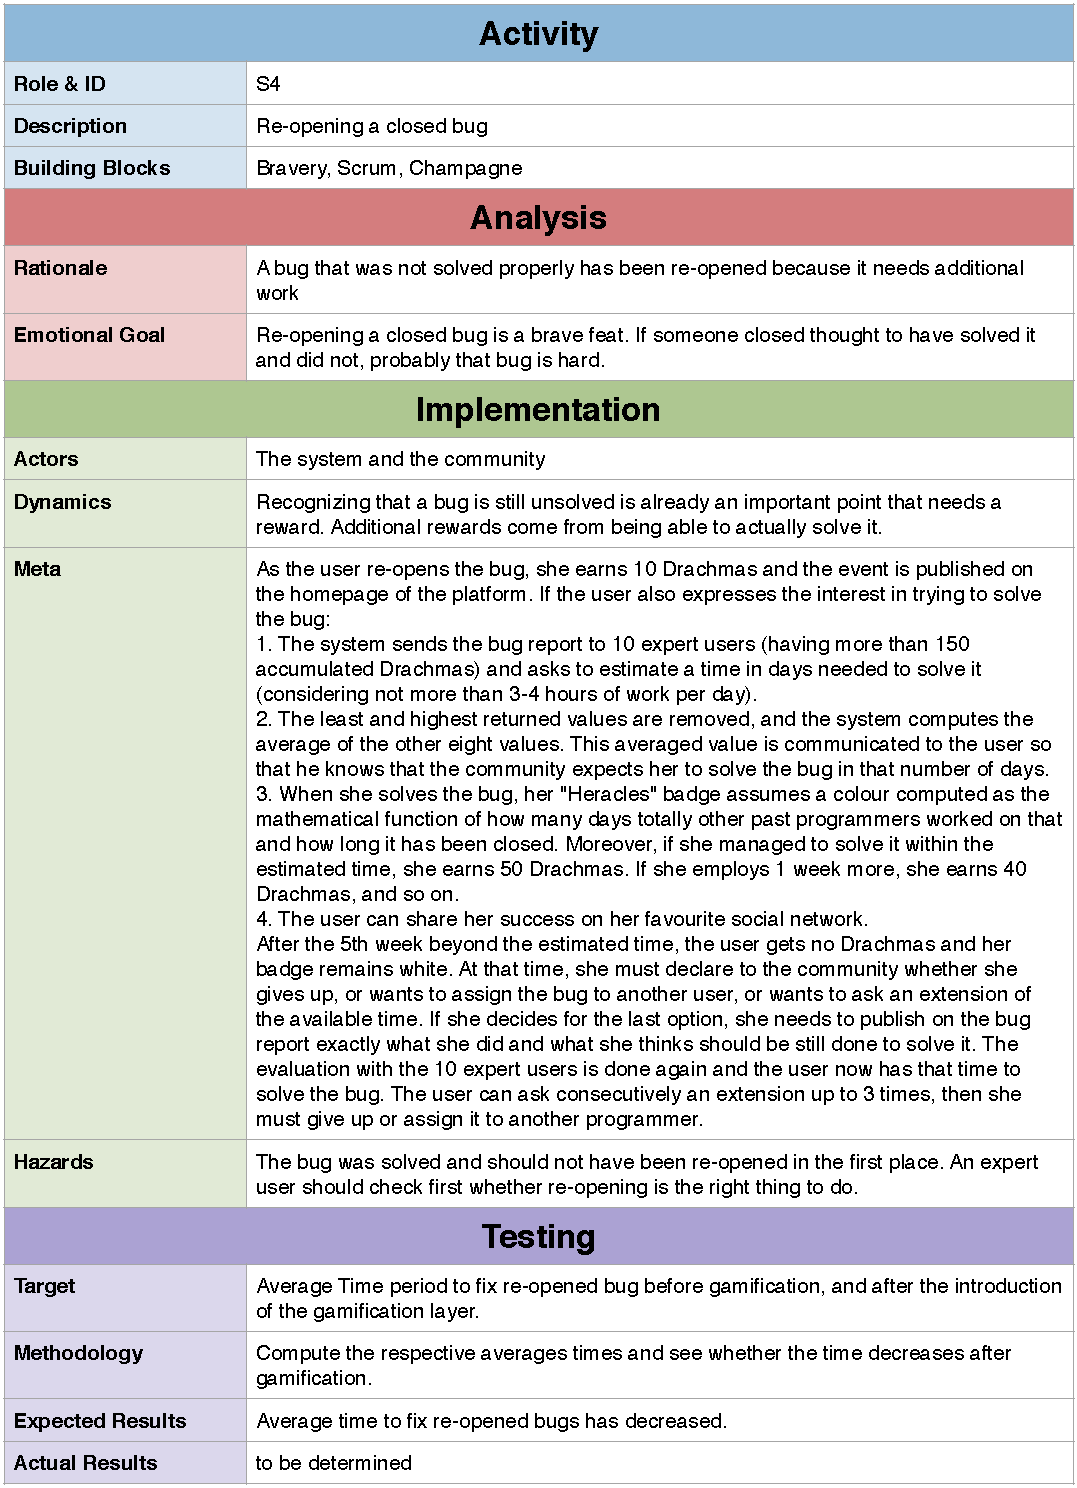
\includegraphics[width=7.7cm]{gamification/act2}
%\caption{Concrete Gamification Activity}
%\label{fig-act2}
%\end{figure}

Due to space reasons we cannot depict all activities; the goal is to clarify that creating activities is a lengthy process which must be done in an iterative way.

\badge{yob_badge} As the player signs up for the game, she enters the magic world of ancient Greece and receives her first reward, the \textbf{Newbie badge} and a small amount of drachmas (the ancient Greek currency), with which the player can buy her avatar some equipment.
The game awards different amounts of Drachmas according to the difficulty of the accomplished task.
This first operation is trivially easy (just registering and give some personal information for the user profile), but it has a special feature: It is the first action that the user does to get into the platform and the first active contact with the community.
Moreover, receiving immediately an unexpected reward works as a bait for the new player who is motivated to add another prize to her collection as soon as possible.

\begin{figure}[t]
\centering
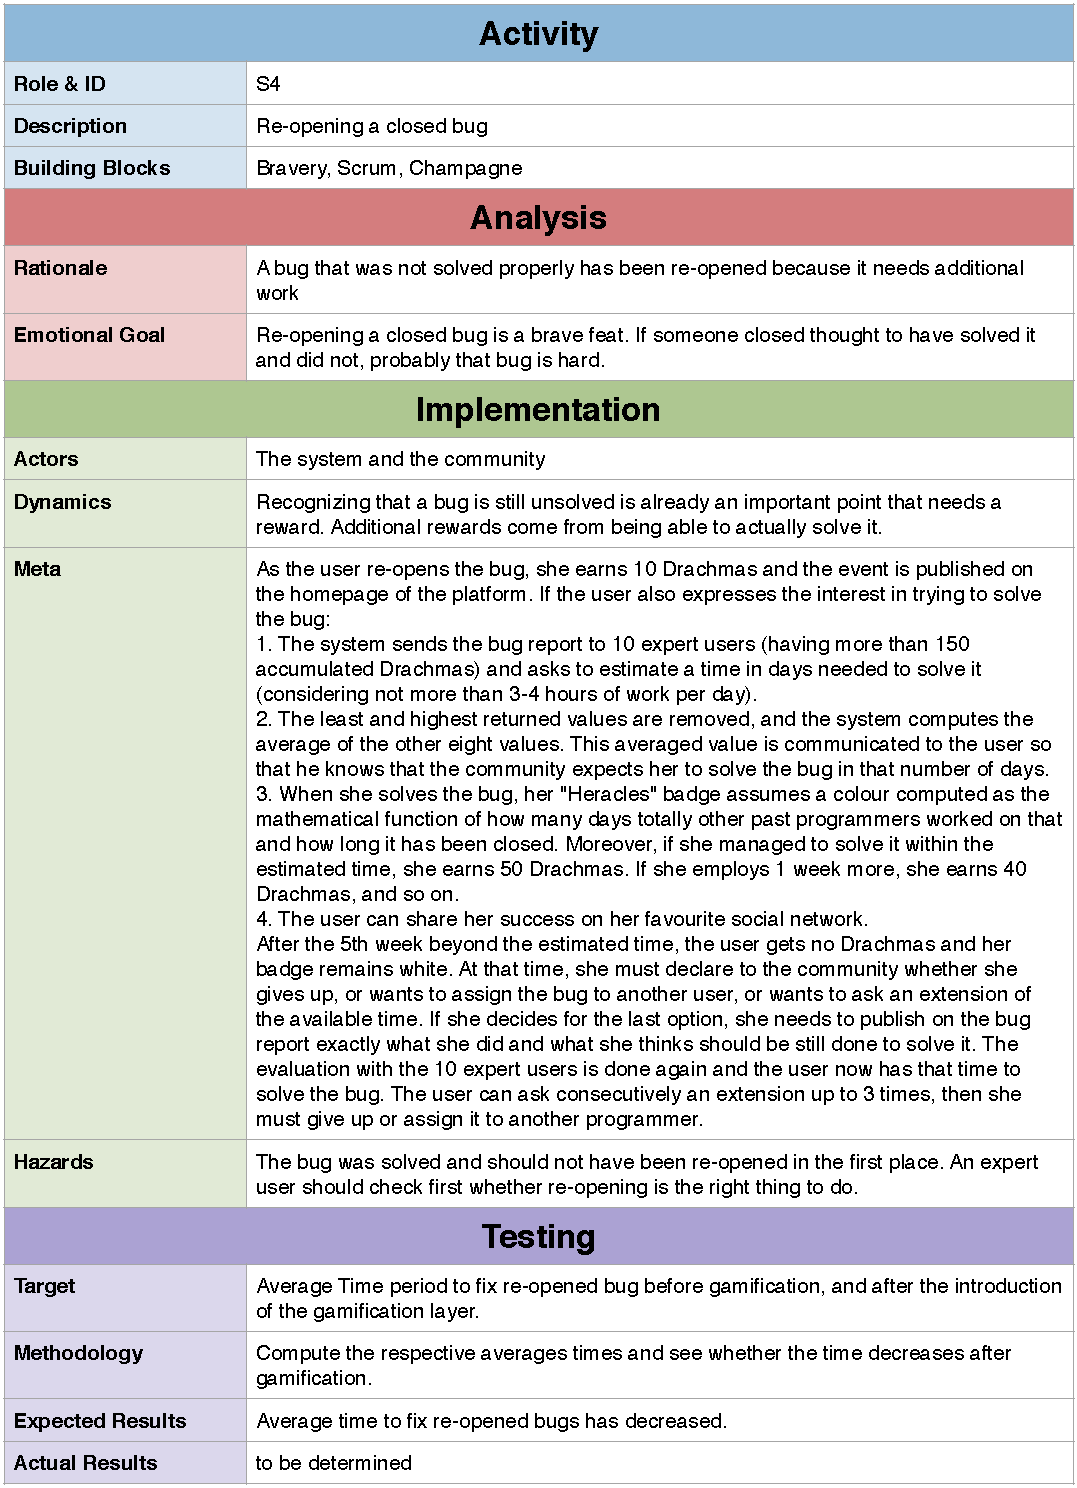
\includegraphics[width=.65\linewidth]{gamification/act2}
\caption{Concrete Gamification Activity}
\label{fig-act2}
\end{figure}

\badge{briefed_badge} The second unexpected reward is quite easy to acquire too: Becoming conscious of the rules holding in the world of Ancient Greece, the player earns the \textbf{Briefed badge}.
She does so by going through a tutorial which explains the bug tracker and the rules of the game.

The system assists the player along the whole path to mastery: It directly furnishes to the user practical tasks that she can afford with her current skills.
While writing a bug report, the system supports the player by using mandatory \textbf{box fields} asking for specific information or suggesting where to look to find it.
It helps reporters to not forget essential information and provides some scaffolding to boost player to mastery.
Motivation is a precious good that some techniques are able to elicit, but at the same time can be shut down easily.
A single apparently insignificant demonstration of disapproval from some other member of the community can hurt a newbie.
\textit{The Myth and De-Bug} avoids such an effect by impeding questions and answers with scores smaller than 0 and avoiding the so-called ``Dislike'' system.

\badge{phidias_badge} A point of strength of this gamification layer is that everyone, from the new user up to administrator, has the chance to propose improvements for the  environment.
The player whose proposal for an extension of the environment has been accepted by the community, gains the \textbf{Phidias badge}.

\badge{tombraider_badge} An open problem of gamification communities (for example Stack Overflow), is keeping the motivation of users high or to recover it when it naturally decreases~\cite{Grant2013}.
We designed badges that level up proportionally with the amount of work performed, \eg \textbf{Tomb Raider} is a badge achievable when a developer explores old posted reports, finds something interesting, and sets the status of the report back to active.

%\badge{heracles_badge}
\noindent
\begin{wrapfigure}{l}{0.07\textwidth}
\centering
\vspace{-18pt}

\includegraphics[width=0.06\textwidth]{gamification/heracles_badge.pdf}
\vspace{-30pt}
\end{wrapfigure}
\textbf{Heracles}\footnote{Heracles was the greatest hero in Greek mythology.
He had incredible courage, physical strength and ingenuity.
Among the many ventures attributed to him, he defeated the Hydra monster, a sea serpent with nine heads.
Every time someone cut one away, it grew anew.
This is a conceptual parallelism with what happens with closed bugs that are reopened.} is a badge of the same nature of Tomb Raider, but is awarded for closing re-opened bugs.

% \pagebreak
Our environment also deals with the issue of {\em balance}.
If a gamification layer is too linear in terms of dispensing mere (and in a way meaningless) points, the danger of pointsification comes up: Users start to hunt for points by performing meaningless and contradictory actions, such as re-opening bugs that do not need to be reopened.
The building block {\em Scrum} is crucial in this case, which means to rely on the community, for example by setting time limits for specific activities.

Also, our environment does not make large use of leaderboards because they are gamification elements that, in a number of cases, may demotivate players.
We designed the leaderboard ``Twenty Top Hoplites of The Week'' by relying on the fact that having a considerably high work rate is an occasional ability.
Since a developer cannot be constantly productive, the leaderboard thus becomes dynamic.

\badge{achilles_badge} When users are on the leaderboards for an extended period of time, they gain the \textbf{Achilles\footnote{We choose for this badge the figure of Achilles, the king of the Myrmidons, son of Zeus and Thesis.
The parallelism with the badge comes from the fact that his most common epithet in Homeric works is ``swift-footed'' because Achilles was known to be very fast at running.} badge} and an amount of bonus Drachmas to refurbish the avatar.

To foster epicness, one of the traits identified by McGonigal as instrumental to gamification, our environment provides a number of places where players can acknowledge the feats of other players.
This happens for instance when a developer closes a difficult bug, or the community reaches a landmark (\eg closing the 1000th bug) collaborating as a team.
The environment also features specific leaderboards, in the form of halls of fame, where important contributors are acknowledged or where productive former newbies are entered into the category ``The New Greek Legends''.

\textit{The Myth and De-bug} is an instance of inducement prizes: Its goals are efficiency, development of creativity, and stimulating collaboration among the community even while competing.
It is also ``cheap'' because it only involves virtual goods, and pays a deep attention to balancing issues.
We just described a possible instantiation of this gamification system.
We could take exactly the same framework, substitute the name of the badges and imprint the game toward modern heroes (Spider Man, Batman, Superman, etc).
They are just fancy names, and we can use the fantasy we like to shape the same gamification dynamics.

\subsection{Example II: The Empire of Gemstones}\label{sec:gamification-example-gems}

The first example was developed in the context of a novel bug tracker we are implementing~\cite{DalS2014a}.
We also devised a number of other software engineering gamification environments, which led to the distillation of the building blocks discussed previously.
We now present another case study of a gamification layer for a software engineering context: Modern Code Reviews.
Due to space limitations we do not present the solution at the same level of detail as the previous example, but focus here mostly on a concept that was only sketched in the previous section: \emph{leveling up}.

Code reviews is a software engineering practice that consists in manually reviewing source code written by other people, to verify and improve the quality of the code.
While the effectiveness of this method has been proven during the years~\cite{Shull2008a}, this practice is often considered expensive, cumbersome, and, as such, difficult to adopt.
Bacchelli and Bird proposed \textit{Modern Code Reviews}~\cite{Bacc2013a}, a code review approach that is informal, tool based, and performed on a frequent basis.
They developed \textit{CodeFlow}, a tool where the user can annotate the source code and interact with other users with a chat.
A developer that wants to propose his code for review has to create a package with the changes, write a brief description and submit it to the \textit{CodeFlow} service.

The area of code reviews still has many open questions, but the \textit{CodeFlow} platform represents the ideal environment to develop a gamification layer to stimulate the amount of motivation necessary to turn code reviews into a habit.

In the context of a code review tool we are currently building in the research group, we designed a gamification environment named \textit{The Empire of Gemstones}, to exploit the parallelism between collecting gemstones and improving the quality of the code.
We employ gems as a virtual currency to reward positive feedback while using proposed solutions.
The number and the type of gems compose a reputation system based on noble titles, used by the system to rank users, which also facilitates the finding of experts in specific areas.

It has been shown~\cite{Bacc2013a} that teams use code reviews for the following purposes: (1) finding defects in the code; (2) improving the code; (3) finding better implementations; (4) transferring knowledge in the group; (5) increasing the team awareness and transparency; and (6) sharing code ownership.

Given the strong implicit collaborative nature of code review tools, we pose a strong accent on blocks that expect interaction with other users, like \emph{Scrum} and \emph{Champagne}.
However, also the motivation of single users can be catalyzed, for example by rewarding quality code, thus suggesting the use of \emph{Bravery} and \emph{Thunderbolt} blocks.

In parallel with a set of badges devised with a similar procedure to the one used to build \textit{The Myth and De-Bug}, we introduce a ``leveling'' mechanism to provide users with a feeling of progression and growth while reviewing the code: Leveling is one of the main drivers of gamification systems, as it fosters positive competition among the players.

By reviewing other's code, a user gets a gem.
The kind of gem depends on the number, size and difficulty of the reviews.
Each gem has a different value according to its rarity, as we see in \tabref{tab-gems}.

\begin{table}[ht]\small
\centering
\caption{Points acquired per 1 gemstone.}
\begin{tabular}{l|r}
\textbf{Gemstone} & \textbf{Points} \\
\hline
\rowcolor{emerald}Emerald & 10\\
\rowcolor{sapphire!40}Sapphire & 9\\
\rowcolor{tanzanite}Tanzanite & 8\\
\rowcolor{aquamarine}Aquamarine & 7\\
\rowcolor{ruby}Ruby & 6\\
\rowcolor{jade}Jade & 5\\
\rowcolor{citrine}Citrine & 4\\
\rowcolor{topaz}Topaz & 3\\
\rowcolor{amethyst}Amethyst & 2\\
\rowcolor{quartz}Quartz & 1\\
\hline
\end{tabular}
\label{pointsgem}
\label{tab-gems}
\end{table}

For example, a reviewer may check some code that includes changes for fifty lines of code over five different files, for which she receives a Jade.
Another user reviews three small changes, each one involving only one file, and she receives three Quartz.
Reviews that spot bugs, that propose a better implementation of the reviewed code (goals 1, 2 and 3) get higher value gems, but since reviewing code also means knowledge transfer (goal 4 and 5), users get a reward even if the review causes no changes.

Submitting code for review implies willingness to collaborate and accept critics, an not being protective of her code (goal 6).
We decided however not to assign gems depending on the outcome of the review to the submitter, to avoid pointsification and because that would suggest an idea of code reviews begin judgmental, which in the long run would discourage a user from submitting his code for review.
A submitter can however still receive badges for particular behaviors, like the \textbf{Collector} badge for users that submit regularly their code, or the \textbf{Houskeeper} for users that submit large numbers of reviews in a short time.

By collecting gems, a user can grow his estate and obtain noble titles which reflect the expertise level in the community, as depicted in \tabref{tab-noble}.
For example, a new user in the team is reviewing many small changes to understand the project he is working on.
He then collects many Quartz, slowly being promoted to Knight after 12 reviews, and Baron after 24.

\begin{table}[t]\small
\centering
\caption{Required number and type of gemstones to obtain noble title.}\label{titles}
% \begin{tabular}{p{0.5cm}p{0.7cm}p{0.7cm}p{0.7cm}p{0.7cm}p{0.7cm}p{0.7cm}p{0.7cm}}
\begin{tabular}{rrrrrrrr}
& \multicolumn{7}{c}{\textbf{Noble Titles}}\\
\cline{2-8}
\multicolumn{1}{l|}{\textbf{Family}} & \cellcolor{gold!100} Prince & \cellcolor{gold!84} Duke & \cellcolor{gold!74} Marquis & \cellcolor{gold!64} Count & \cellcolor{gold!52} Viscount & \cellcolor{gold!40} Baron & \cellcolor{gold!28} Knight\\
\hline
\rowcolor{emerald} \multicolumn{1}{l|}{Emerald} & 27 & 21 & 16 & 12 & 9 & 6 & 3\\
\rowcolor{sapphire!40} \multicolumn{1}{l|}{Sapphire} & 34 & 27 & 21 & 16 & 12 & 8 & 4\\
\rowcolor{tanzanite} \multicolumn{1}{l|}{Tanzanite} & 41 & 33 & 26 & 20 & 15 & 10 & 5\\
\rowcolor{aquamarine} \multicolumn{1}{l|}{Aquamarine} & 48 & 39 & 31 & 24 & 18 & 12 & 6\\
\rowcolor{ruby} \multicolumn{1}{l|}{Ruby} & 55 & 45 & 36 & 28 & 21 & 14 & 7\\
\rowcolor{jade} \multicolumn{1}{l|}{Jade} & 62 & 51 & 41 & 32 & 24 & 16 & 8\\
\rowcolor{citrine} \multicolumn{1}{l|}{Citrine} & 69 & 57 & 46 & 36 & 27 & 18 & 9\\
\rowcolor{topaz} \multicolumn{1}{l|}{Topaz} & 76 & 63 & 51 & 40 & 30 & 20 & 10\\
\rowcolor{amethyst} \multicolumn{1}{l|}{Amethyst} & 83 & 69 & 56 & 44 & 33 & 22 & 11\\
\rowcolor{quartz} \multicolumn{1}{l|}{Quartz} & 90 & 75 & 61 & 48 & 36 & 24 & 12\\
\hline
\end{tabular}
\label{tab-noble}
\end{table}

The avatar of the player in this environment is then also depicted in a gameful way, such as a house which gets more beautiful as the player obtains more gems.
In the code review tool, these avatars could then be shown to other reviewers when they log into the tool.

As we anticipated, the leveling mechanism is useful in stimulating positive competition among team members.
Given the context of code reviews, which by definition happen inside the same team, company or community, we believe that the level system is particularly effective in leveraging the interpersonal bonds and endorse motivation in improving the quality of the code.


%%%%%%%%%%%%%%%%%%%%%%%%%%%%%%%%%%%%%
\section{Evaluating Gamified Systems}\label{sec:gamification-evaluation}
%%%%%%%%%%%%%%%%%%%%%%%%%%%%%%%%%%%%%

Once a system is gamified, we need to be able to measure the impact of the gamification, and how much it contributed to reach the {\em business objectives}.
It is crucial not to confuse business objectives with game objectives: with the coexistence of ``serious'' and ``fun'' layers, it is easy to exchange the goals of the two aspects, thus misjudging the effects.

In building our framework, we included a testing section, whose purpose is to decide at design time a procedure to state how successful the game elements applied to each single activity are.
But, a system is more than the mere sum of all its parts: As such, testing all the single elements does not imply the success of the whole gamification system, exactly as in software development we need integration tests.

We propose five methods to assess the general performance of the gamification on top of a software engineering context: \emph{success metrics}, \emph{analytics}, \emph{conflicts}, \emph{jen ratio} and \emph{survey}.
The first three focus on technical aspects to consider the business objectives, while the the last two consider emotional aspects.
Due to their subjective nature, we cannot get a precise measure of emotional response of the users and compare the obtained values in a consistent way.
The relative metrics have then to consider the imprecise nature of the data they deal with.


\subsubsection{Success Metrics}

The first approach is to define a set of goals at design time, and verify them after the system has been in production for a while.
We recommend to make a list of the goals of the gamification system, define success metrics (number of new users in the last month, average activity increase per user, \etc) tailored to specific activities and verifiable with usage data.
A long enough timeframe must be used to perceive a noticeable change: People's habits take a while to deal with novelties.
A significative amount of data must be collected before and after the introduction of the gamification layer to enable before/after testing.


\subsubsection{Analytics}

A useful metric is represented by the measure of users interacting with the enviroment: \emph{Daily Active Users (DAU)} is the number of unique users that interact with the software tool during a day, while \emph{Monthly Active Users (MAU)} is the average number of unique users that interacted with the software tool in the previous 30 days.
By computing the ratio $\frac{\textit{DAU}}{\textit{MAU}}$ we have the trend of usage of the software tool in a given moment.
The result of such a ratio goes from 0 to 1: It is close to 1 when the tool is engaging, and it is close to 0 when its popularity is decreasing.
$\frac{\textit{DAU}}{\textit{MAU}}$ is a relevant parameter to keep under observation because, if it increases the number of active users is growing; if it decreases they are decreasing.


\subsubsection{Conflicts}

Some gamification elements can create conflicts with existing elements on the system.
Listing and prioritizing the conflicts, also by listening to the users through forums and mailing list, is helpful.
If a conflict persists, the involved gamification elements should be pulled out of the environment, as user dissatisfaction can be harmful to the whole community.


\subsubsection{Jen Ratio}

Establish two sets of interactions in the user community: \emph{positive interactions} (\eg virtual gifts, acknowledgements), and \emph{negative interactions} (\eg misbehaviours, rude comments).
Compute the \emph{Jen Ratio}: total positive interactions among users over the total negative interactions, in a given period of time and context.
The outcome is between 0 and 1.
The jen ratio assesses how positive the attitude of the users is: the closer to 1, the better the social well-being of the community.


\subsubsection{Survey}

Selected users, of all expertise levels, should be periodically surveyed, where key questions should not only regard technical aspects, but also emotional aspects.


\subsubsection{}

Beyond the use of these metrics, it is important to perform an evaluation on the effective gain of the system, to quantify how the use of gamification impacted the activity of the users and if it brought actual benefits.
For example, in a bug tracking system we can measure the number of bug reports opened and closed every day, the average duration of a bug report and the number of bug reports that a user examines.
However, it is clear that such metrics are domain specific, and have to be calibrated for each different gamification context.


\section{Discussion}\label{sec:gamification-discussion}

In this section we propose our reflections on the lesson we learned developing our work.
We then discuss how we think our work can be improved.


\subsection{Reflections}

The examples in \secref{sec:gamification-framework} hint at a fact that should not be disregarded about gamification: To create such environments is a far from trivial endeavor.
The reasoning that goes into creating thematic environments, the way that leveling is handled, how and when awards and badges should be assigned, is a strongly iterative process.
One might be tempted to bypass such a labor-intensive work by using the simplest solution, which is to award points and to base the leveling on such points.
However, apart from the danger of pointsification, there is another risk, which we define as ``stalling'': If the gamification layer is not constantly revisited, maintained, and evolved, it risks to quickly become obsolete, and therefore will not only be ignored by the users, but it might even cause decreased participation.
Last, there is also the issue of adoption: Since many software engineering activities are done with tools that come from vendors or open-source communities, one would have to convince those to introduce the gamification layer on top of their tools.
It is doubtful that this would happen if there is no substantial evidence that the gamification layer actually works, which brings us back to the concern of evaluating such environments.

% \subsection{Related Work}
%
% There have been few other efforts in this direction so far.
% Passos \textit{et al.}~\cite{PassosMNC11} proposed to gamify the phases of software lifecycle by splitting the whole process into tasks, and setting achievements for their completion.
% While this is an interesting approach, it is essentially a \emph{pointsification}, and as such puts too much emphasis on the rewards, thus being ineffective on the long run.
% Singer and Schneider performed a study on the gamification of commit messages~\cite{sing2012}: they managed to influence the workflow of the students in the experiment, improving the workflow.
% They however received both positive and negative comments.
% Dubois and Tamburelli~\cite{Dubois2013a} pointed out that software projects often produce mediocre quality artefacts, do not respect the terms for milestones, or exceed the financial budget.
% They claimed that gamification could represent a solution to the issue, but only outlined a possible approach to gamification based on the three steps analysis, integration, and evaluation.
% Probably still being in the inception phase they did not provide concrete suggestions or a systematic set of recommendations.
%
% We believe this paper provides a starting point to approach the gamification of software engineering in a systematic way and also provided recommendations on how to evaluate it.

\subsection{Next Steps}

We composed the gamification layers presented in this chapter as part of the process to understand the basic concepts of gamification and practically see what is meaningful or what should be highlighted as dangerous.
The main result of our work were the gamification framework and the ten essential building blocks to use as a reference in building the system, but the presented scenarios are actual software engineering problems currently investigated by researchers.

The focus of our work revolves around the activities performed by the users.
However, further insights can come from considering the different types of users in a community, to avoid the negative effect of marginalizing some users.
For example, Vasilescu \etal studied the difference between men and women in approaching---and leaving---a community~\cite{vasi2012}, while Koivisto \etal showed how the ease of use of gamification tends to decline with age~\cite{koiv2014}.


%%%%%%%%%%%%%%%%%%%%%%%%%%%%%%%%%%%%%%%%%%
\section{Outline}\label{sec:gamification-summary}
%%%%%%%%%%%%%%%%%%%%%%%%%%%%%%%%%%%%%%%%%%

We presented a critical overview on the relevant literature on gamification, and proposed a framework to support the design of a gamification layer to support software engineering tasks.
We showed how to implement practical actions to successfully gamify a system, and we distilled ten essential \emph{building blocks} that represent basic elements to be considered when designing gamification activities.
We then discussed two example software gamification environments highlighting a number of challenges.
Last, we outlined a proposal on how gamification systems can be evaluated.


%The solutions developed to build \textit{The Myth and De-Bug} were designed with an actual use scenario in mind, and are being integrated into \textit{ShoreLine}, a comprehensive platform to manage bug reports developed for the \textit{Pharo}\footnote{https://pharo.org} community.
%\textit{Pharo} is a programming language inspired by \textit{Smalltalk}, with an active development and an energetic community.
Our hope is that integrating gamification elements in software engineering will allow developers to build tools where the potential of gamification is leveraged to foster collaboration and contributions by the community.
In that sense: The game has just started.


\part{Conclusion}
  %!TEX root = ../tommaso-thesis.tex
%!TEX spellcheck = en_US

% \chapter{Conclusion}\label{ch:conclusion}
\coolchapter{Conclusion}{}{ch:conclusion}


Software development produces large amounts of raw data pertaining to the evolution of a system.
The majority of this data is dismissed as a byproduct of the development process and lost.
Even when fragments of this data are saved and used, they are flattened in textual format, complicating automated analyses and reducing its reliability.
We are convinced that such data is an invaluable asset in supporting developers, to understand both how a system works and how users interact with it.
We think that it can become the central component in the design of the next generation of issue tracking systems.

We introduced our work by showing an overview of the efforts by researchers and practitioners to improve the organization and fruition of bug reports.
We presented a set of approaches and tools to propose an improved style for collecting bug reports.
We implemented our core idea of automatic and reified data collection in \sln, a platform to record runtime exceptions and to gather domain-specific information about specific parts of the system.
We developed our tools in \pha, a dynamic language with a tightly integrated IDE and a strong community.
The use of \pha helped us prototype our tools and quickly test different ideas, allowing us to easily access all the details of the system.
Interacting with the \pha community allowed us to get feedback on the tools we deployed, and to perform qualitative studies to get a preliminary evaluation on our approaches.

The data we collected showed us that failure data can be exploited to support program comprehension, debugging, and optimization of existing systems.
This in turn can help reduce the time spent on maintenance, thus containing development costs.


\section{Visualization of Bug Data}

During the preliminary phase of our work we performed a visual inspection of existing bug repositories, looking for patterns and hidden properties that could help accessing the stored information.
Later on, we employed again visualizations to navigate the data we collected.
We believe that, given the amount of data generated during development, visualizations are an effective means to summarize the activity on a project and provide a selective and layered point of view on specific aspects of the system.


\subsection{Reading Between the Lines}

In \chref{ch:visualize}, we presented \ib, a web platform to visually inspect the contents of existing issue tracking systems.
We ascertained that bug reports contain information that is not properly conveyed with a mere textual representation.
We exploited the structured parts of a bug report (\eg its metadata) to build a view of the life and evolution of a bug report, highlighting its lifetime and the events of which it is composed.
We were able to spot interesting cases of bug reports, like stale bugs that are opened but did not receive any recent activity, or bug reports reopened multiple times.
This result suggested us that there is room for improvement in accessing the information that we store about software defects.



\subsection{Narrating the Evolution of a System}

In \chref{ch:blend} we presented \tool{Blend}, a tool to display and merge multiple data sources about a system.
We used the city metaphor~\cite{Wett2011a} to depict the entities in the \pha system and their properties.
We used the stack traces collected with \sln, our tool to collect information about runtime errors, we extracted the changes in the \pha system during one year of development, and we integrated the user interaction data dataset provided by Minelli \etal~\cite{Mine2017a}.
We then colored each entity combining different colors to represent the data collected about that entity.
From the resulting visualization we could navigate the evolution of the system from a historical perspective, and tell stories about development that can help development decisions or highlight the need for maintenance.


\section{Collecting Failure Information}

The second step in our work consisted in augmenting the reliability of bug reports by augmenting them with automatically collecting failure data.

\subsection{Collecting Stack Traces}

In \chref{ch:stacktraces} we presented our crowdstacking approach: the collection of stack traces from the community to spot recurring errors and understand the usage of a system.
We introduced \slr, our tool for implementing this approach in the \pha system, and analyzed the $7,532$ stack traces that we collected between June and November 2014.
We used the data we collected to show the activity of the users on the system, thus showing the components that can be optimized or the ones that need improvement.
We then searched the issue tracking system of \pha looking for references to the entities in the stack traces.
We found that for some stack traces we were able to find an existing bug report.
We believe that the approach of automatically providing contextual feedback when an error occurs can greatly improve the experience of the user on a software system and save time.


\subsection{Reifying Bug Reports}

In \chref{ch:reified} we extended the approach presented in \chref{ch:stacktraces} by allowing developers to collect not only stack traces, but also domain specific information about a software component.
By employing \emph{collectors}, a developer can specify when an error is interesting to collect and specify the rules to collect it.
Collecting the information in its object form, rather that flattening it into a textual representation, allows us to start a conversation with the system that can unveil the hidden properties among the entities in the software.



\section{Modeling an Issue Tracking System}

In the final part of our dissertation we discussed how to improve the experience of users and developers in the issue tracking system.
We observed the problem from two different points of view: how to model a bug report to ease the life of reporting users, and how to engage users and developers in participating in the debugging activity.


\subsection{The Model of a Bug Report}

In \chref{ch:model} we explored the usage of existing issue tracking systems for projects from the \emph{Apache} and \emph{Mozilla} foundations.
We conducted a survey to understand what users perceive as difficult to provide when submitting a bug report.
We then showed that an increasing number of fields in a bug report has little relation with the lifetime of a bug report.
We believe that this study suggests us that a redesign of an issue tracking system should start from simplifying the existing one, rather than adding more textual information.


\subsection{Gamification}

In \chref{ch:gamification} we explored the possibility of boosting user engagement when using an issue tracking system by means of \emph{gamification}, the use of game elements in non-gaming contexts.
We presented an overview on the history of gamification and its evolution over time.
We proposed a framework for systematically gamifying software engineering, posing particular care in highlighting the pitfalls that must be avoided when dealing with gamification.
We think that gamification can become a valuable tool, if used to highlight and improve the interactions already existing on a community and not to enforce a specific behavior.
It can support the management of software projects, help welcoming new users, and motivating the expert ones.



\section{Limitations and Future Work}

We believe that developing our research project we only scratched the surface of the possible improvements that we can apply to current development methodologies.
We provide an overview of the directions that we would like to further investigate, while also discussing the limitation of the approaches we employed.

\subsubsection{User Interface}

We used the data we collected to generate knowledge on the system.
We did not, however, consider the process from a user interface perspective.
We are aware that presenting the information to the user in a meaningful and non-intrusive fashion is as crucial as providing correct information: We therefore think that investigating how to display such contextual information to the user is a crucial aspect that should be tackled.


\subsubsection{Evaluation}

Given the size of the task that we considered, we were able to evaluate our approaches in small contexts, mostly from a tool-driven, qualitative point of view.
We believe that a full evaluation of a new issue tracking system, if possible, would require years to complete.
Still, a deeper study of the interaction of the various improvement of the development process could shed light on further directions in rethinking issue tracking systems.


\subsubsection{Privacy}

During our research project we collected a large amount of stack traces from developers performing real development tasks.
We were careful in allowing our users to avoid submitting sensible information, but we believe that further efforts in this direction could ease the adoption of such tools and allow the collection of more useful data while safeguarding the privacy and the intellectual property of developers.


\subsubsection{Integration With the System}
Data collection alone is not enough to provide a smoother development experience.
By having access to structured data, we can integrate such information with development tools, for example by recreating the context where a bug occurred with a single click on a website.



\section{Closing Words}

In this dissertation we showed that data generated during software failures carries useful information in understanding and improving a system.
We argued that this information should not be discarded, but rather promoted to first-class citizen in the development process by treating it with customized representation, rather that using plain text.
This would allow the creation of contextual tools such as visual browsers, recommender systems, or automated build systems.
To support software development further, however, it is essential that development tools (\ie the IDE) integrates such data to create a \emph{holistic} experience.

We see our thesis as a first step in rethinking the idea of bug report, to build smarter issue tracking systems that support development in a deeper and integrated fashion.





%\appendix %optional, use only if you have an appendix


\backmatter

\chapter{Glossary} %optional

%\bibliographystyle{alpha}
\bibliographystyle{dcu}
%\bibliographystyle{plainnat}
\bibliography{biblio}

\cleardoublepage
\theindex %optional, use only if you have an index, must use
	  %\makeindex in the preamble

\end{document}
